%
% This document describes the ee know-how used in Qucs.
%
% Copyright (C) 2003, 2004, 2005 Stefan Jahn <stefan@lkcc.org>
% Copyright (C) 2004 Michael Margraf <Michael.Margraf@alumni.TU-Berlin.DE>
%
% Permission is granted to copy, distribute and/or modify this document
% under the terms of the GNU Free Documentation License, Version 1.1
% or any later version published by the Free Software Foundation.
%

\documentclass[10pt,a4paper,oneside]{report}
\usepackage{a4wide}
\usepackage{epsfig}
\usepackage{array}
\usepackage{amsmath}
\usepackage{amsfonts}
\usepackage{stmaryrd}
\usepackage[amssymb]{SIunits}
\usepackage{graphics}
\usepackage{psfrag}
\usepackage{relsize}
\usepackage[section]{placeins}
\usepackage{listings}

% Compatibility code for LaTeX and pdfTeX.
\newif\ifpdf
\ifx\pdfoutput\undefined
  \pdffalse
\else
  \pdfoutput=1
  \pdftrue
\fi

% Only evaluated if run using pdfTeX.
\ifpdf
\usepackage[pdftex,
	a4paper,
	bookmarks,
	bookmarksopen=true,
	bookmarksnumbered=true,
	pdfpagemode=UseNone,
	baseurl=(http://qucs.sourceforge.net),
	pdfstartview=FitH,
	colorlinks,
	linkcolor=black,
	urlcolor=black,
	citecolor=black,
	backref=false,
	plainpages=false,
	pagebackref=false]{hyperref}
\pdfcompresslevel 9
\pdfinfo {
  /Title   (Qucs)
  /Subject (Technical Papers)
  /Author  (Stefan Jahn and Michael Margraf and Vincent Habchi
	and Raimund Jacob)
}
\fi

% Title page definitions.
\makeatletter
\renewcommand{\maketitle}{\begin{titlepage}%
    \setlength{\parindent}{0pt}
    \vspace*{3cm}
    \begin{flushleft}
      \textbf{\begin{huge}\@title\end{huge}}
    \end{flushleft}
    \hrule height 3pt
    \begin{flushright}
      \begin{LARGE}Technical Papers\end{LARGE}
    \end{flushright}
    \vfill
    \begin{flushright}
      \begin{Large}\@author\end{Large}
    \end{flushright}
    \hrule height 3pt
    \vspace*{24pt}

Copyright \copyright{} 2003, 2004, 2005 Stefan Jahn
\textless stefan@lkcc.org\textgreater

Copyright \copyright{} 2003, 2004, 2005 Michael Margraf
\textless michael.margraf@alumni.tu-berlin.de\textgreater

Copyright \copyright{} 2004, 2005 Vincent Habchi, F5RCS
\textless 10.50@free.fr\textgreater

Copyright \copyright{} 2005 Raimund Jacob
\textless raimi@lkcc.org\textgreater

    \vspace*{12pt}

Permission is granted to copy, distribute and/or modify this document
under the terms of the GNU Free Documentation License, Version 1.1 or
any later version published by the Free Software Foundation.  A copy
of the license is included in the section entitled "GNU Free
Documentation License".

    \vspace*{1cm}

    \end{titlepage}%
    \setcounter{footnote}{0}%
}
\makeatother

\author{Stefan Jahn\\Michael Margraf\\Vincent Habchi\vspace*{6pt}\\Raimund Jacob}
\title{Qucs}
\date{}

% Here finally starts everything.
\begin{document}

\maketitle

\tableofcontents

\setlength{\parindent}{0pt}
\newpage

%
% This document contains the chapter about S-parameters.
%
% Copyright (C) 2003, 2004 Stefan Jahn <stefan@lkcc.org>
% Copyright (C) 2004 Michael Margraf <Michael.Margraf@alumni.TU-Berlin.DE>
%
% Permission is granted to copy, distribute and/or modify this document
% under the terms of the GNU Free Documentation License, Version 1.1
% or any later version published by the Free Software Foundation.
%

\chapter{Scattering parameters}
%\addcontentsline{toc}{chapter}{Scattering parameters}

\section{Introduction and definition}
%\addcontentsline{toc}{section}{Introduction and definition}

Voltage and current are hard to measure at high frequencies.  Short
and open circuits (used by definitions of most n-port parameters) are
hard to realize at high frequencies.  Therefore, microwave engineers
work with so-called scattering parameters (S parameters), that uses
waves and matched terminations (normally $50 \Omega$).  This procedure
also minimizes reflection problems.

\addvspace{12pt}

A (normalized) wave is defined as ingoing wave $\underline{a}$ or
outgoing wave $\underline{b}$:

\begin{equation}
\underline{a} = \frac{u+Z_0\cdot i}{\sqrt{\text{Re}(Z_0)}} \qquad
\underline{b} = \frac{u-Z_0^*\cdot i}{\sqrt{\text{Re}(Z_0)}}
\label{equ:waves}
\end{equation}
where $u$ is (effective) voltage, $i$ (effective) current and $Z_0$ reference
impedance. The waves are related to power in the following way.
\begin{equation}
P = \left( |\underline{a}|^2 - |\underline{b}|^2 \right)
\end{equation}
Sometimes waves are defined with peak voltages and peak currents.
The only difference that appears then is the relation to power:
\begin{equation}
P = \frac{1}{2}\cdot \left( |\underline{a}|^2 - |\underline{b}|^2 \right)
\end{equation}
Now, characterizing an n-port is straight-forward:
\begin{equation}
\begin{pmatrix}
\underline{b}_1\\
\vdots\\
\underline{b}_n\\
\end{pmatrix}
=
\begin{pmatrix}
\underline{S}_{11} & \ldots & \underline{S}_{1n}\\
\vdots & \ddots & \vdots\\
\underline{S}_{n1} & \ldots & \underline{S}_{nn}\\
\end{pmatrix}
\cdot
\begin{pmatrix}
\underline{a}_1\\
\vdots\\
\underline{a}_n\\
\end{pmatrix}
\end{equation}


\section{Computing with S-parameters}
%\addcontentsline{toc}{section}{Computing with S-parameters}

\subsection{Recalculating $\mathbf{50\ohm}$-S-parameters for arbitrary port impedances}
%\addcontentsline{toc}{subsection}{Recalculating $50\ohm$-S-parameters for arbitrary port impedances}

During S-parameter usage it sometimes appears to have not all components
in a circuit normalized to the same impedance. But calculations can only
be performed with all ports being normalized to the same impedance. In
the field of high
frequency techniques this is usually $50\ohm$.  In order to transform
to different port impedances, the following computation must be applied
to the resulting S-parameter matrix.

\begin{equation}
\left[\underline{N'}\right] =
\left(\left[\underline{S}\right] - \left[\underline{R}\right]\right) \cdot
\left(\left[\underline{E}\right] - \left[\underline{R}\right] \cdot \left[\underline{S}\right]\right)^{-1}
\end{equation}

\begin{equation}
\underline{N}_{nm} = \underline{N'}_{nm}\cdot \sqrt{\dfrac{Z_m}{Z_n}\cdot
\dfrac{Z_{n,before}}{Z_{m,before}}}\cdot
\dfrac{Z_n + Z_{n,before}}{Z_m + Z_{m,before}}
\end{equation}

With

\addvspace{12pt}

\begin{tabular}{rll}
$Z_{n}$ & = & norm impedance after the normalizing process\\& &\\
$Z_{n,before}$ & = & norm impedance before the normalizing process\\& &\\
$\left[\underline{E}\right]$ & = &
$\begin{pmatrix}
1 & 0 & \ldots & 0\\
0 & 1 & \ldots & 0\\
\vdots & \vdots & \ddots & \vdots\\
0 & 0 & \ldots & 1\\
\end{pmatrix}$
identity matrix\\& &\\
$\left[\underline{S}\right]$ & = & original $50\ohm$-S-parameter matrix\\& &\\
$\left[\underline{N}\right]$ & = & recalculated scattering matrix\\& &\\
$\left[\underline{R}\right]$ & = &
$\begin{pmatrix}
\underline{r}(Z_{1}) & 0 & \ldots & 0\\
0 & \underline{r}(Z_{2}) & \ldots & 0\\
\vdots & \vdots & \ddots & \vdots\\
0 & 0 & \ldots & \underline{r}(Z_{n})\\
\end{pmatrix}$
reflection coefficient matrix\\& &\\
$\underline{r}(Z_{n})$ & = &
$\dfrac{Z_{n} - Z_{n,before}}{Z_{n} + Z_{n,before}}$
reflection coefficient of impedance at port n\\& &\\
\end{tabular}

And furthermore

\addvspace{12pt}

\begin{tabular}{rll}
$\left[\underline{X}\right]^{-1}$ & = & 
inverted matrix of $\left[\underline{X}\right]$\\& &\\
$\underline{X}_{nm}$ & = & 
element of matrix $\left[\underline{X}\right]$ at row n and column m\\& &\\
\end{tabular}

\subsection{S-parameters in CAE programs}
%\addcontentsline{toc}{subsection}{S-parameters in CAE programs}
\label{sec:SparameterCAE}

The most common task of a simulation program is to compute the S
parameters of an arbitrary network that consists of many elementary
components connected to each other.  To perform this, one can build a
large matrix containing the S parameters of all components and then
use matrix operations to solve it.  However this method needs heavy
algorithms.  A more elegant possibility was published in
\cite{Compton}. Each step computes only one connection and so unites
two connected components to a single S parameter block.  This
procedure has to be done with every connection until there is only one
block left whose S parameters therefore are the simulation result.

\addvspace{12pt}

Connecting port $k$ of circuit $(\underline{S})$ with port $l$ of
circuit $(\underline{T})$, the new S-parameters are
\begin{equation}
\underline{S}'_{ij} = \underline{S}_{ij} +
      \frac{\underline{S}_{kj}\cdot \underline{T}_{ll}\cdot \underline{S}_{ik}}
           {1-\underline{S}_{kk}\cdot \underline{T}_{ll}}
\label{eq:connectSij}
\end{equation}
with $i$ and $j$ both being ports of $(\underline{S})$.  Furthermore, it is
\begin{equation}
\underline{S}'_{mj} =
      \frac{\underline{S}_{kj}\cdot \underline{T}_{ml}}
           {1-\underline{S}_{kk}\cdot \underline{T}_{ll}}
\label{eq:connectSmj}
\end{equation}
with $m$ being a port of the circuit $(\underline{T})$.  If two ports
of the same circuit $(\underline{S})$ are connected, the new
S-parameters are
\begin{equation}
\underline{S}'_{ij} = \underline{S}_{ij} +
      \frac{ \underline{S}_{kj}\cdot \underline{S}_{il}\cdot (1-\underline{S}_{lk})
           + \underline{S}_{lj}\cdot \underline{S}_{ik}\cdot (1-\underline{S}_{kl})
           + \underline{S}_{kj}\cdot \underline{S}_{ll}\cdot \underline{S}_{ik}
           + \underline{S}_{lj}\cdot \underline{S}_{kk}\cdot \underline{S}_{il}}
           {(1-\underline{S}_{kl})\cdot (1-\underline{S}_{lk}) - \underline{S}_{kk}\cdot \underline{S}_{ll}}.
\label{eq:iconnectSij}
\end{equation}

If more than two ports are connected at a node, one have to insert one
or more ideal tee components.  Its S parameters write as follows.
\begin{equation}
\begin{pmatrix}
\underline{S}
\end{pmatrix}
= \dfrac{1}{3}\cdot
\begin{pmatrix}
-1 &  2 &  2\\
 2 & -1 &  2\\
 2 &  2 & -1\\
\end{pmatrix}
\end{equation}
For optimisation reasons it may be desireable to insert a cross if
at least four components are connected at one node. Its
S parameters writes as follows.
\begin{equation}
\begin{pmatrix}
\underline{S}
\end{pmatrix}
= \dfrac{1}{2}\cdot
\begin{pmatrix}
-1 &  1 &  1 &  1\\
 1 & -1 &  1 &  1\\
 1 &  1 & -1 &  1\\
 1 &  1 &  1 & -1\\
\end{pmatrix}
\end{equation}


\addvspace{12pt}


The formulas \eqref{eq:connectSij}, \eqref{eq:connectSmj} and
\eqref{eq:iconnectSij} were obtained using the ``nontouching-loop''
rule being an analytical method for solving a flow graph.  A few basic
definitions have to be understood.

\addvspace{12pt}

A ``path'' is a series of branches into the same direction with no
node touched more than once.  A paths value is the product of the
coefficients of the branches.  A ``loop'' is formed when a path starts
and finishes at the same node.  A ``first-order'' loop is a path
coming to closure with no node passed more than once.  Its value is
the product of the values of all branches encountered on the route.  A
``second-order'' loop consists of two first-order loops not touching
each other at any node.  Its value is calculated as the product of the
values of the two first-order loops.  Third- and higher-order loops
are three or more first-order loops not touching each other at any
node.

\addvspace{12pt}

The nontouching-loop rule can be applied to solve any flow graph.  In
the following equation in symbolic form $T$ represents the ratio of
the dependent variable in question and the independent variable.

\begin{equation}
T = \dfrac{
\begin{array}{r}
P_{1}\cdot\left(1 - \Sigma L_{1}^{(1)} + \Sigma L_{2}^{(1)} - \Sigma L_{3}^{(1)} + \ldots\right) +
P_{2}\cdot\left(1 - \Sigma L_{1}^{(2)} + \Sigma L_{2}^{(2)} - \Sigma L_{3}^{(2)} + \ldots\right)\\
+ P_{3}\cdot\left(1 - \Sigma L_{1}^{(3)} + \Sigma L_{2}^{(3)} - \Sigma L_{3}^{(3)} + \ldots\right) +
P_{4}\cdot\left(1 - \ldots\right) + \ldots
\end{array}
}{1 - \Sigma L_{1} + \Sigma L_{2} - \Sigma L_{3} + \ldots}
\label{eq:ntrule}
\end{equation}

In eq. \eqref{eq:ntrule} $\Sigma L_{1}$ stands for the sum of all
first-order loops, $\Sigma L_{2}$ is the sum of all second-order
loops, and so on.  $P_{1}$, $P_{2}$, $P_{3}$ etc., stand for the
values of all paths that can be found from the independent variable to
the dependent variable.  $\Sigma L_{1}^{(1)}$ denotes the sum of those
first-order loops which do not touch (hence the name) the path of
$P_{1}$ at any node, $\Sigma L_{2}^{(1)}$ denotes then the sum of
those second-order loops which do not touch the path $P_{1}$ at any
point, $\Sigma L_{1}^{(2)}$ consequently denotes the sum of those
first-order loops which do not touch the path of $P_{2}$ at any point.
Each path is multiplied by the factor in parentheses which involves
all the loops of all orders that the path does not touch.

\addvspace{12pt}

When connecting two different networks the signal flow graph in
fig. \ref{fig:sconnectgraph} is used to compute the new S-parameters.
With equally reference impedances on port $k$ and port $l$ the
relations $\underline{a}_{k} = \underline{b}_{l}$ and
$\underline{a}_{l} = \underline{b}_{k}$ are satisfied.

\begin{figure}[ht]
\begin{center}
\includegraphics[width=0.8\linewidth]{sconnectgraph}
\end{center}
\caption{signal flow graph of a joint between ports $k$ and $l$ on different networks}
\label{fig:sconnectgraph}
\end{figure}
\FloatBarrier

There is only one first-order loop (see fig. \ref{fig:sconnectloop})
within this signal flow graph.  This loops value yields to
\begin{equation}
L_{11} = \underline{S}_{kk}\cdot \underline{T}_{ll}
\end{equation}

\begin{figure}[ht]
\begin{center}
\includegraphics[height=3.1cm]{sconnectloop}
\end{center}
\caption{loops in the signal flow graph when connecting ports $k$ and $l$ on different networks}
\label{fig:sconnectloop}
\end{figure}
\FloatBarrier

The paths that can be found from the independent variable
$\underline{a}_{j}$ to the dependent variable $\underline{b}_{i}$ (as
depicted in fig. \ref{fig:sconnectpath}) can be written as
\begin{align}
P_{1} &= \underline{S}_{kj}\cdot \underline{T}_{ll} \cdot \underline{S}_{ik}\\
P_{2} &= \underline{S}_{ij}
\end{align}

\begin{figure}[ht]
\begin{center}
\includegraphics[height=3.1cm]{sconnectpath}
\end{center}
\caption{paths in the signal flow graph when connecting ports $k$ and $l$ on different networks}
\label{fig:sconnectpath}
\end{figure}
\FloatBarrier

Applying the nontouching-loop rule, i.e. eq. \eqref{eq:ntrule}, gives
the new S-parameter $\underline{S}'_{ij}$
\begin{equation}
\begin{split}
\underline{S}'_{ij} = \dfrac{\underline{b}_{i}}{\underline{a}_{j}} &= \dfrac{P_{1}\cdot\left(1 - L_{11}\right) + P_{2}\cdot 1}{1 - L_{11}}\\
&= \dfrac{\underline{S}_{ij}\cdot\left(1 - \underline{S}_{kk}\cdot \underline{T}_{ll}\right) + \underline{S}_{kj}\cdot \underline{T}_{ll}\cdot \underline{S}_{ik}}{1 - \underline{S}_{kk}\cdot \underline{T}_{ll}}
= \underline{S}_{ij} + \dfrac{\underline{S}_{kj}\cdot \underline{T}_{ll}\cdot \underline{S}_{ik}}{1 - \underline{S}_{kk}\cdot \underline{T}_{ll}}
\end{split}
\end{equation}

The only path that can be found from the independent variable
$\underline{a}_{j}$ to the dependent variable $\underline{b}_{m}$ (as
depicted in fig. \ref{fig:sconnectpath}) can be written as
\begin{equation}
P_{1} = \underline{S}_{kj}\cdot \underline{T}_{ml}
\end{equation}

Thus the new S-parameter $\underline{S}'_{mj}$ yields to
\begin{equation}
\underline{S}'_{mj} = \dfrac{\underline{b}_{m}}{\underline{a}_{j}}
= \dfrac{P_{1}\cdot 1}{1 - L_{11}}
= \dfrac{\underline{S}_{kj}\cdot \underline{T}_{ml}}{1 - \underline{S}_{kk}\cdot \underline{T}_{ll}}
\end{equation}

When connecting the same network the signal flow graph in
fig. \ref{fig:siconnectgraph} is used to compute the new S-parameters.
With equally reference impedances on port $k$ and port $l$ the
relations $\underline{a}_{k} = \underline{b}_{l}$ and
$\underline{a}_{l} = \underline{b}_{k}$ are satisfied.

\begin{figure}[ht]
\begin{center}
\includegraphics[width=0.55\linewidth]{siconnectgraph}
\end{center}
\caption{signal flow graph of a joint between ports $k$ and $l$ on the same network}
\label{fig:siconnectgraph}
\end{figure}
\FloatBarrier

There are three first-order loops and a second-order loop (see
fig. \ref{fig:siconnectloop}) within this signal flow graph.  These
loops' values yield to
\begin{align}
L_{11} &= \underline{S}_{kk}\cdot \underline{S}_{ll}\\
L_{12} &= \underline{S}_{kl}\\
L_{13} &= \underline{S}_{lk}\\
L_{21} &= L_{12}\cdot L_{13} = \underline{S}_{kl}\cdot \underline{S}_{lk}
\end{align}

\begin{figure}[ht]
\begin{center}
\includegraphics[height=3.7cm]{siconnectloop}
\end{center}
\caption{loops in the signal flow graph when connecting ports $k$ and $l$ on the same network}
\label{fig:siconnectloop}
\end{figure}
\FloatBarrier

There are five different paths that can be found from the independent
variable $\underline{a}_{j}$ to the dependent variable
$\underline{b}_{i}$ (as depicted in fig. \ref{fig:siconnectpath})
which can be written as
\begin{align}
P_{1} &= \underline{S}_{kj}\cdot \underline{S}_{ll}\cdot \underline{S}_{ik}\\
P_{2} &= \underline{S}_{kj}\cdot \underline{S}_{il}\\
P_{3} &= \underline{S}_{lj}\cdot \underline{S}_{ik}\\
P_{4} &= \underline{S}_{ij}\\
P_{5} &= \underline{S}_{lj}\cdot \underline{S}_{kk}\cdot \underline{S}_{il}
\end{align}

\begin{figure}[ht]
\begin{center}
\includegraphics[height=7.4cm]{siconnectpath}
\end{center}
\caption{paths in the signal flow graph when connecting ports $k$ and $l$ on the same network}
\label{fig:siconnectpath}
\end{figure}
\FloatBarrier

Thus the new S-parameter $\underline{S}'_{ij}$ yields to
\begin{equation}
\begin{split}
\underline{S}'_{ij}
&= \dfrac{P_{1} + P_{2}\cdot\left(1 - L_{13}\right) + P_{3}\cdot\left(1 - L_{12}\right) + P_{4}\cdot\left(1 - \left(L_{11} + L_{12} + L_{13}\right) + L_{21}\right) + P_{5}}{1 - \left(L_{11} + L_{12} + L_{13}\right) + L_{21}}\\
&= P_{4} + \dfrac{P_{1} + P_{2}\cdot\left(1 - L_{13}\right) + P_{3}\cdot\left(1 - L_{12}\right) + P_{5}}{1 - \left(L_{11} + L_{12} + L_{13}\right) + L_{21}}\\
&= \underline{S}_{ij} + \dfrac{\underline{S}_{kj}\cdot \underline{S}_{ll}\cdot \underline{S}_{ik} + \underline{S}_{kj}\cdot \underline{S}_{il} \cdot\left(1 - \underline{S}_{lk}\right) + \underline{S}_{lj}\cdot \underline{S}_{ik}\cdot\left(1 - \underline{S}_{kl}\right) + \underline{S}_{lj}\cdot \underline{S}_{kk}\cdot \underline{S}_{il}}{1 - \left(\underline{S}_{kk}\cdot \underline{S}_{ll} + \underline{S}_{kl} + \underline{S}_{lk}\right) + \underline{S}_{kl}\cdot \underline{S}_{lk}}\\
&= \underline{S}_{ij} + \dfrac{\underline{S}_{kj}\cdot \underline{S}_{ll}\cdot \underline{S}_{ik} + \underline{S}_{kj}\cdot \underline{S}_{il} \cdot\left(1 - \underline{S}_{lk}\right) + \underline{S}_{lj}\cdot \underline{S}_{ik}\cdot\left(1 - \underline{S}_{kl}\right) + \underline{S}_{lj}\cdot \underline{S}_{kk}\cdot \underline{S}_{il}}{\left(1 - \underline{S}_{kl}\right)\cdot \left(1 - \underline{S}_{lk}\right) - \underline{S}_{kk}\cdot \underline{S}_{ll}}
\end{split}
\end{equation}

This short introduction to signal flow graphs and their solution using
the nontouching-loop rule verifies the initial formulas used to
compute the new S-parameters for the reduced subnetworks.


\subsection{Differential S-parameter ports}
%\addcontentsline{toc}{subsection}{Differential S-parameter ports}
\label{sec:diffSParam}

The implemented algorithm for the S-parameter analysis calculates
S-parameters in terms of the ground node.  In order to allow
differential S-parameters as well it is necessary to insert an ideal
impedance transformer with a turns ratio of 1:1 between the
differential port and the device under test.

\begin{figure}[ht]
\begin{center}
\includegraphics[width=12cm]{differential}
\end{center}
\caption{transformation of differential port into single ended port}
\label{fig:differential}
\end{figure}
\FloatBarrier

The S-parameter matrix of the inserted ideal transformer being a three
port device can be written as follows.

\begin{equation}
\begin{pmatrix}
\underline{S}
\end{pmatrix}
= \dfrac{1}{3}\cdot
\begin{pmatrix}
1 & 2 & -2\\
2 & 1 & 2\\
-2 & 2 & 1\\
\end{pmatrix}
\end{equation}

This transformation can be applied to each S-parameter port in a
circuit regardless whether it is actually differential or not.

\addvspace{12pt}

It is also possible to do the impedance transformation within this step
(for S-parameter ports with impedances different than $50\ohm$). This can
be done by using a transformer with an impedance ration of

\begin{equation}
r=T^2=\frac{50\ohm}{Z}
\end{equation}

With $Z$ being the S-parameter port impedance. The S-parameter matrix of
the inserted ideal transformer now writes as follows.

\begin{equation}
\begin{pmatrix}
\underline{S}
\end{pmatrix}
= \dfrac{1}{2\cdot Z_0+Z}\cdot
\begin{pmatrix}
2\cdot Z_0-Z              & 2\cdot\sqrt{Z_0\cdot Z}  & -2\cdot\sqrt{Z_0\cdot Z}\\
2\cdot\sqrt{Z_0\cdot Z}   & Z                        & 2\cdot Z_0\\
-2\cdot\sqrt{Z_0\cdot Z}  & 2\cdot Z_0               & Z\\
\end{pmatrix}
\end{equation}

With $Z$ being the new S-parameter port impedance and $Z_0$ being $50\ohm$.

\section{Matrix conversions}
%\addcontentsline{toc}{section}{Matrix conversions}
\label{sec:SparameterConversion}

When dealing with S-parameter analyses it may be necessary or
convenient to convert the resulting scattering parameter matrix into
other matrix representations used in microwave engineering.

\subsection{S-Parameter to impedance matrix}
%\addcontentsline{toc}{subsection}{S-Parameter to impedance matrix}

Converting a scattering parameter matrix to an impedance matrix is
done by the following formula.

\begin{equation}
\left[
\underline{Z}
\right]
=
\left[
\underline{G}_{ref}
\right]^{-1}
\cdot
\left(
\left[\underline{E}\right] - \left[\underline{S}\right]
\right)^{-1}
\cdot
\left(
\left[\underline{S}\right] \cdot \left[\underline{Z}_{ref}\right] + \left[\underline{Z}_{ref}\right]^{*}
\right)
\cdot
\left[\underline{G}_{ref}\right]
\end{equation}

With

\addvspace{12pt}

\begin{tabular}{rll}
$\left[\underline{E}\right]$ & = &
$\begin{bmatrix}
1 & 0 & \ldots & 0\\
0 & 1 & \ldots & 0\\
\vdots & \vdots & \ddots & \vdots\\
0 & 0 & \ldots & 1\\
\end{bmatrix}$
identity matrix\\& &\\
$\left[\underline{S}\right]$ & = & original S-parameter matrix\\& &\\
$\left[\underline{Z}\right]$ & = & resulting impedance matrix\\& &\\
$\left[\underline{Z}_{ref}\right]$ & = &
$\left[\underline{E}\right] \cdot Z_{0}$\\& &\\
$\left[\underline{G}_{ref}\right]$ & = &
$\left[\underline{E}\right] \cdot 
\dfrac{1}{2\cdot \sqrt{\left| \text{Re}\left(Z_{0}\right)\right|}}$\\& &\\
$Z_{0}$ & = & reference impedance (by default $50\ohm$)\\& &\\
\end{tabular}

And furthermore

\addvspace{12pt}

\begin{tabular}{rll}
$\left[\underline{X}\right]^{-1}$ & = & 
inverted matrix of $\left[\underline{X}\right]$\\& &\\
$\left[\underline{X}\right]^{*}$ & = & 
complex conjugated matrix of $\left[\underline{X}\right]$\\& &\\
\end{tabular}

\subsection{S-Parameter to admittance matrix}
%\addcontentsline{toc}{subsection}{S-Parameter to admittance matrix}

Converting a scattering parameter matrix to an admittance matrix can
be achieved by computing the following formula.

\begin{equation}
\left[
\underline{Y}
\right]
=
\left[
\underline{G}_{ref}
\right]^{-1}
\cdot
\left(
\left[\underline{S}\right] \cdot \left[\underline{Z}_{ref}\right] + \left[\underline{Z}_{ref}\right]^{*}
\right)^{-1}
\cdot
\left(
\left[\underline{E}\right] - \left[\underline{S}\right]
\right)
\cdot
\left[\underline{G}_{ref}\right]
\end{equation}

With

\addvspace{12pt}

\begin{tabular}{rll}
$\left[\underline{E}\right]$ & = &
$\begin{bmatrix}
1 & 0 & \ldots & 0\\
0 & 1 & \ldots & 0\\
\vdots & \vdots & \ddots & \vdots\\
0 & 0 & \ldots & 1\\
\end{bmatrix}$
identity matrix\\& &\\
$\left[\underline{S}\right]$ & = & original S-parameter matrix\\& &\\
$\left[\underline{Y}\right]$ & = & resulting admittance matrix\\& &\\
$\left[\underline{Z}_{ref}\right]$ & = &
$\left[\underline{E}\right] \cdot Z_{0}$\\& &\\
$\left[\underline{G}_{ref}\right]$ & = &
$\left[\underline{E}\right] \cdot 
\dfrac{1}{2\cdot \sqrt{\left| \text{Re}\left(Z_{0}\right)\right|}}$\\& &\\
$Z_{0}$ & = & reference impedance (by default $50\ohm$)\\& &\\
\end{tabular}

And furthermore

\addvspace{12pt}

\begin{tabular}{rll}
$\left[\underline{X}\right]^{-1}$ & = & 
inverted matrix of $\left[\underline{X}\right]$\\& &\\
$\left[\underline{X}\right]^{*}$ & = & 
complex conjugated matrix of $\left[\underline{X}\right]$\\& &\\
\end{tabular}

\subsection{Impedance matrix to scattering parameter matrix}
%\addcontentsline{toc}{subsection}{Impedance matrix to scattering parameter matrix}

Converting an impedance matrix to a scattering parameter matrix is
done by the following formula.

\begin{equation}
\left[
\underline{S}
\right]
=
\left[
\underline{G}_{ref}
\right]
\cdot
\left(
\left[\underline{Z}\right] - \left[\underline{Z}_{ref}\right]^{*}
\right)
\cdot
\left(
\left[\underline{Z}\right] + \left[\underline{Z}_{ref}\right]
\right)^{-1}
\cdot
\left[\underline{G}_{ref}\right]^{-1}
\end{equation}

With

\addvspace{12pt}

\begin{tabular}{rll}
$\left[\underline{E}\right]$ & = &
$\begin{bmatrix}
1 & 0 & \ldots & 0\\
0 & 1 & \ldots & 0\\
\vdots & \vdots & \ddots & \vdots\\
0 & 0 & \ldots & 1\\
\end{bmatrix}$
identity matrix\\& &\\
$\left[\underline{S}\right]$ & = & resulting S-parameter matrix\\& &\\
$\left[\underline{Z}\right]$ & = & original impedance matrix\\& &\\
$\left[\underline{Z}_{ref}\right]$ & = &
$\left[\underline{E}\right] \cdot Z_{0}$\\& &\\
$\left[\underline{G}_{ref}\right]$ & = &
$\left[\underline{E}\right] \cdot 
\dfrac{1}{2\cdot \sqrt{\left| \text{Re}\left(Z_{0}\right)\right|}}$\\& &\\
$Z_{0}$ & = & reference impedance (by default $50\ohm$)\\& &\\
\end{tabular}

And furthermore

\addvspace{12pt}

\begin{tabular}{rll}
$\left[\underline{X}\right]^{-1}$ & = &
inverted matrix of $\left[\underline{X}\right]$\\& &\\
$\left[\underline{X}\right]^{*}$ & = & 
complex conjugated matrix of $\left[\underline{X}\right]$\\& &\\
\end{tabular}

\subsection{Admittance matrix to scattering parameter matrix}
%\addcontentsline{toc}{subsection}{Admittance matrix to scattering parameter matrix}

Converting an admittance matrix to a scattering parameter matrix is
done by the following formula.

\begin{equation}
\left[
\underline{S}
\right]
=
\left[
\underline{G}_{ref}
\right]
\cdot
\left(
\left[\underline{E}\right] - \left[\underline{Z}_{ref}\right]^{*} \cdot \left[\underline{Y}\right]
\right)
\cdot
\left(
\left[\underline{E}\right] + \left[\underline{Z}_{ref}\right] \cdot \left[\underline{Y}\right]
\right)^{-1}
\cdot
\left[\underline{G}_{ref}\right]^{-1}
\end{equation}

With

\addvspace{12pt}

\begin{tabular}{rll}
$\left[\underline{E}\right]$ & = &
$\begin{bmatrix}
1 & 0 & \ldots & 0\\
0 & 1 & \ldots & 0\\
\vdots & \vdots & \ddots & \vdots\\
0 & 0 & \ldots & 1\\
\end{bmatrix}$
identity matrix\\& &\\
$\left[\underline{S}\right]$ & = & resulting S-parameter matrix\\& &\\
$\left[\underline{Y}\right]$ & = & original admittance matrix\\& &\\
$\left[\underline{Z}_{ref}\right]$ & = &
$\left[\underline{E}\right] \cdot Z_{0}$\\& &\\
$\left[\underline{G}_{ref}\right]$ & = &
$\left[\underline{E}\right] \cdot 
\dfrac{1}{2\cdot \sqrt{\left| \text{Re}\left(Z_{0}\right)\right|}}$\\& &\\
$Z_{0}$ & = & reference impedance (by default $50\ohm$)\\& &\\
\end{tabular}

And furthermore

\addvspace{12pt}

\begin{tabular}{rll}
$\left[\underline{X}\right]^{-1}$ & = & 
inverted matrix of $\left[\underline{X}\right]$\\& &\\
$\left[\underline{X}\right]^{*}$ & = & 
complex conjugated matrix of $\left[\underline{X}\right]$\\& &\\
\end{tabular}

\subsection{Impedance matrix to admittance matrix}
%\addcontentsline{toc}{subsection}{Impedance matrix to admittance matrix}

Converting an impedance matrix to an admittance matrix is done by the
following formula.

\begin{equation}
\left[
\underline{Y}
\right]
=
\left[
\underline{Z}
\right]^{-1}
\end{equation}

With

\addvspace{12pt}

\begin{tabular}{rll}
$\left[\underline{Y}\right]$ & = & resulting admittance matrix\\& &\\
$\left[\underline{Z}\right]$ & = & original impedance matrix\\& &\\
\end{tabular}

And furthermore

\addvspace{12pt}

\begin{tabular}{rll}
$\left[\underline{X}\right]^{-1}$ & = & 
inverted matrix of $\left[\underline{X}\right]$\\& &\\
\end{tabular}

\subsection{Admittance matrix to impedance matrix}
%\addcontentsline{toc}{subsection}{Admittance matrix to impedance matrix}

Converting an admittance matrix to an impedance matrix is done by the
following formula.

\begin{equation}
\left[
\underline{Z}
\right]
=
\left[
\underline{Y}
\right]^{-1}
\end{equation}

With

\addvspace{12pt}

\begin{tabular}{rll}
$\left[\underline{Z}\right]$ & = & resulting impedance matrix\\& &\\
$\left[\underline{Y}\right]$ & = & original admittance matrix\\& &\\
\end{tabular}

And furthermore

\addvspace{12pt}

\begin{tabular}{rll}
$\left[\underline{X}\right]^{-1}$ & = & 
inverted matrix of $\left[\underline{X}\right]$\\& &\\
\end{tabular}

\subsection{Two-Port transformations}
%\addcontentsline{toc}{subsection}{Two-Port transformations}

\subsubsection{Two-Port matrix conversion based on current and voltage}
%\addcontentsline{toc}{subsubsection}{Two-Port matrix conversion based on current and voltage}

\begin{figure}[ht]
\begin{center}
\includegraphics[height=3cm]{twoportiv}
\end{center}
\caption{twoport definition using current and voltage}
\label{fig:twoportiv}
\end{figure}
\FloatBarrier

There are five different matrix forms for the correlations between the
quantities at the transmission twoport shown in
fig. \ref{fig:twoportiv}, each having its special meaning when
connecting twoports with each other.

\begin{itemize}

\item Y-parameters (also called admittance parameters)
\begin{equation}
\begin{pmatrix}
\underline{I}_{1}\\
\underline{I}_{2}
\end{pmatrix}
=
\begin{pmatrix}
\underline{Y}_{11} & \underline{Y}_{12}\\
\underline{Y}_{21} & \underline{Y}_{22}
\end{pmatrix}
\cdot
\begin{pmatrix}
\underline{V}_{1}\\
\underline{V}_{2}
\end{pmatrix}
\end{equation}

\item Z-parameters (also called impedance parameters)
\begin{equation}
\begin{pmatrix}
\underline{V}_{1}\\
\underline{V}_{2}
\end{pmatrix}
=
\begin{pmatrix}
\underline{Z}_{11} & \underline{Z}_{12}\\
\underline{Z}_{21} & \underline{Z}_{22}
\end{pmatrix}
\cdot
\begin{pmatrix}
\underline{I}_{1}\\
\underline{I}_{2}
\end{pmatrix}
\end{equation}

\item H-parameters (also called hybrid parameters)
\begin{equation}
\begin{pmatrix}
\underline{V}_{1}\\
\underline{I}_{2}
\end{pmatrix}
=
\begin{pmatrix}
\underline{H}_{11} & \underline{H}_{12}\\
\underline{H}_{21} & \underline{H}_{22}
\end{pmatrix}
\cdot
\begin{pmatrix}
\underline{I}_{1}\\
\underline{V}_{2}
\end{pmatrix}
\end{equation}

\item G-parameters (also called C-parameters)
\begin{equation}
\begin{pmatrix}
\underline{I}_{1}\\
\underline{V}_{2}
\end{pmatrix}
=
\begin{pmatrix}
\underline{G}_{11} & \underline{G}_{12}\\
\underline{G}_{21} & \underline{G}_{22}
\end{pmatrix}
\cdot
\begin{pmatrix}
\underline{V}_{1}\\
\underline{I}_{2}
\end{pmatrix}
\end{equation}

\item A-parameters (also called chain or ABCD-parameters)
\begin{equation}
\begin{pmatrix}
\underline{V}_{1}\\
\underline{I}_{1}
\end{pmatrix}
=
\begin{pmatrix}
\underline{A}_{11} & \underline{A}_{12}\\
\underline{A}_{21} & \underline{A}_{22}
\end{pmatrix}
\cdot
\begin{pmatrix}
\underline{V}_{2}\\
-\underline{I}_{2}
\end{pmatrix}
\end{equation}

\end{itemize}

\begin{center}
\begin{figure}[ht]
\setlength{\fboxsep}{5pt}
\begin{tabular}{|c|c|c|c|}
\hline
\setlength{\fboxrule}{0pt}
\fbox{\begin{minipage}[t]{0.22\linewidth}
\centering
parallel-parallel connection\\[1ex]
\includegraphics[height=2.5cm]{twoportpp}
\end{minipage}}
&
\begin{minipage}[t]{0.21\linewidth}
\centering
series-series connection\\[1ex]
\includegraphics[height=2.5cm]{twoportss}
\end{minipage}
&
\begin{minipage}[t]{0.21\linewidth}
\centering
series-parallel connection\\[1ex]
\includegraphics[height=2.5cm]{twoportps}
\end{minipage}
&
\begin{minipage}[t]{0.21\linewidth}
\centering
parallel-series connection\\[1ex]
\includegraphics[height=2.5cm]{twoportsp}
\end{minipage}
\\
\hline
\multicolumn{4}{c}{\vline
\setlength{\fboxrule}{0pt}
\fbox{\begin{minipage}[t]{0.85\linewidth}
\centering
cascaded twoports\\[1ex]
\includegraphics[height=1.3cm]{twoportch}
\end{minipage}}
}\vline
\\
\hline
\end{tabular}
\end{figure}
\FloatBarrier
\end{center}

Basically there are five different kinds of twoport connections.
Using the corresponding twoport matrix representations, complicated
networks can be analysed by connecting elementary twoports.  The
linear correlations between the complex currents and voltages rms
values of a twoport are described by four complex twoport parameters
(i.e. the twoport matrix).  These parameters are used to describe the
AC behaviour of the twoport.

\begin{itemize}
\item parallel-parallel connection: use Y-parameters: $Y = Y_{1} + Y_{2}$
\item series-series connection: use Z-parameters: $Z = Z_{1} + Z_{2}$
\item series-parallel connection: use H-parameters: $H = H_{1} + H_{2}$
\item parallel-series connection: use G-parameters: $G = G_{1} + G_{2}$
\item chain connection: use A-parameters: $A = A_{1}\cdot A_{2}$
\end{itemize}

\setlength{\fboxsep}{4pt}
\def\a{0.15\linewidth}
\begin{tabular}{|c|c|c|c|c|c|}
\hline
& A & Y & Z & H & G\\
\hline
A & 
\makebox[\a][c]{$\begin{array}{cc}A_{11}&A_{12}\vspace{4pt}\\A_{21}&A_{22}\end{array}$} &
\setlength{\fboxrule}{0pt}
\fbox{\makebox[\a][c]{$\begin{array}{cc}\dfrac{-Y_{22}}{Y_{21}}&\dfrac{-1}{Y_{21}}\vspace{4pt}\\\dfrac{-\Delta Y}{Y_{21}}&\dfrac{-Y_{11}}{Y_{21}}\end{array}$}} &
\makebox[\a][c]{$\begin{array}{cc}\dfrac{Z_{11}}{Z_{21}}&\dfrac{\Delta Z}{Z_{21}}\vspace{4pt}\\\dfrac{1}{Z_{21}}&\dfrac{Z_{22}}{Z_{21}}\end{array}$} &
\makebox[\a][c]{$\begin{array}{cc}\dfrac{-\Delta H}{H_{21}}&\dfrac{-H_{11}}{H_{21}}\vspace{4pt}\\\dfrac{-H_{22}}{H_{21}}&\dfrac{-1}{H_{21}}\end{array}$} &
\makebox[\a][c]{$\begin{array}{cc}\dfrac{1}{G_{21}}&\dfrac{G_{22}}{G_{21}}\vspace{4pt}\\\dfrac{G_{11}}{G_{21}}&\dfrac{\Delta G}{G_{21}}\end{array}$}\\
\hline
Y & 
\setlength{\fboxrule}{0pt}
\fbox{\makebox[\a][c]{$\begin{array}{cc}\dfrac{A_{22}}{A_{12}}&\dfrac{-\Delta A}{A_{12}}\vspace{4pt}\\\dfrac{-1}{A_{12}}&\dfrac{A_{11}}{A_{12}}\end{array}$}} &
\makebox[\a][c]{$\begin{array}{cc}Y_{11}&Y_{12}\vspace{4pt}\\Y_{21}&Y_{22}\end{array}$} & 
\makebox[\a][c]{$\begin{array}{cc}\dfrac{Z_{22}}{\Delta Z}&\dfrac{-Z_{12}}{\Delta Z}\vspace{4pt}\\\dfrac{-Z_{21}}{\Delta Z}&\dfrac{Z_{11}}{\Delta Z}\end{array}$} &
\makebox[\a][c]{$\begin{array}{cc}\dfrac{1}{H_{11}}&\dfrac{-H_{12}}{H_{11}}\vspace{4pt}\\\dfrac{H_{21}}{H_{11}}&\dfrac{\Delta H}{H_{11}}\end{array}$} &
\makebox[\a][c]{$\begin{array}{cc}\dfrac{\Delta G}{G_{22}}&\dfrac{G_{12}}{G_{22}}\vspace{4pt}\\\dfrac{-G_{21}}{G_{22}}&\dfrac{1}{G_{22}}\end{array}$}\\
\hline
Z & 
\setlength{\fboxrule}{0pt}
\fbox{\makebox[\a][c]{$\begin{array}{cc}\dfrac{A_{11}}{A_{21}}&\dfrac{\Delta A}{A_{21}}\vspace{4pt}\\\dfrac{1}{A_{21}}&\dfrac{A_{22}}{A_{21}}\end{array}$}} &
\makebox[\a][c]{$\begin{array}{cc}\dfrac{Y_{22}}{\Delta Y}&\dfrac{-Y_{12}}{\Delta Y}\vspace{4pt}\\\dfrac{-Y_{21}}{\Delta Y}&\dfrac{Y_{11}}{\Delta Y}\end{array}$} &
\makebox[\a][c]{$\begin{array}{cc}Z_{11}&Z_{12}\vspace{4pt}\\Z_{21}&Z_{22}\end{array}$} & 
\makebox[\a][c]{$\begin{array}{cc}\dfrac{\Delta H}{H_{22}}&\dfrac{H_{12}}{H_{22}}\vspace{4pt}\\\dfrac{-H_{21}}{H_{22}}&\dfrac{1}{H_{22}}\end{array}$} &
\makebox[\a][c]{$\begin{array}{cc}\dfrac{1}{G_{11}}&\dfrac{-G_{12}}{G_{11}}\vspace{4pt}\\\dfrac{G_{21}}{G_{11}}&\dfrac{\Delta G}{G_{11}}\end{array}$}\\
\hline
H & 
\setlength{\fboxrule}{0pt}
\fbox{\makebox[\a][c]{$\begin{array}{cc}\dfrac{A_{12}}{A_{22}}&\dfrac{\Delta A}{A_{22}}\vspace{4pt}\\\dfrac{-1}{A_{22}}&\dfrac{A_{21}}{A_{22}}\end{array}$}} &
\makebox[\a][c]{$\begin{array}{cc}\dfrac{1}{Y_{11}}&\dfrac{-Y_{12}}{Y_{11}}\vspace{4pt}\\\dfrac{Y_{21}}{Y_{11}}&\dfrac{\Delta Y}{Y_{11}}\end{array}$} &
\makebox[\a][c]{$\begin{array}{cc}\dfrac{\Delta Z}{Z_{22}}&\dfrac{Z_{12}}{Z_{22}}\vspace{4pt}\\\dfrac{-Z_{21}}{Z_{22}}&\dfrac{1}{Z_{22}}\end{array}$} &
\makebox[\a][c]{$\begin{array}{cc}H_{11}&H_{12}\vspace{4pt}\\H_{21}&H_{22}\end{array}$} & 
\makebox[\a][c]{$\begin{array}{cc}\dfrac{G_{22}}{\Delta G}&\dfrac{-G_{12}}{\Delta G}\vspace{4pt}\\\dfrac{-G_{21}}{\Delta G}&\dfrac{G_{11}}{\Delta G}\end{array}$}\\
\hline
G & 
\setlength{\fboxrule}{0pt}
\fbox{\makebox[\a][c]{$\begin{array}{cc}\dfrac{A_{21}}{A_{11}}&\dfrac{-\Delta A}{A_{11}}\vspace{4pt}\\\dfrac{1}{A_{11}}&\dfrac{A_{12}}{A_{11}}\end{array}$}} &
\makebox[\a][c]{$\begin{array}{cc}\dfrac{\Delta Y}{Y_{22}}&\dfrac{Y_{12}}{Y_{22}}\vspace{4pt}\\\dfrac{-Y_{21}}{Y_{22}}&\dfrac{1}{Y_{22}}\end{array}$} &
\makebox[\a][c]{$\begin{array}{cc}\dfrac{1}{Z_{11}}&\dfrac{-Z_{12}}{Z_{11}}\vspace{4pt}\\\dfrac{Z_{21}}{Z_{11}}&\dfrac{\Delta Z}{Z_{11}}\end{array}$} &
\makebox[\a][c]{$\begin{array}{cc}\dfrac{H_{22}}{\Delta H}&\dfrac{-H_{12}}{\Delta H}\vspace{4pt}\\\dfrac{-H_{21}}{\Delta H}&\dfrac{H_{11}}{\Delta H}\end{array}$} &
\makebox[\a][c]{$\begin{array}{cc}G_{11}&G_{12}\vspace{4pt}\\G_{21}&G_{22}\end{array}$}\\
\hline
\end{tabular}

\subsubsection{Two-Port matrix conversion based on signal waves}
%\addcontentsline{toc}{subsubsection}{Two-Port matrix conversion based on signal waves}

\begin{figure}[ht]
\begin{center}
\includegraphics[height=3cm]{twoportab}
\end{center}
\caption{twoport definition using signal waves}
\label{fig:twoportab}
\end{figure}
\FloatBarrier

There are two different matrix forms for the correlations between the
quantities at the transmission twoport shown in
fig. \ref{fig:twoportab}.

\begin{itemize}

\item S-parameters (also called scattering parameters)
\begin{equation}
\begin{pmatrix}
\underline{b}_{1}\\
\underline{b}_{2}
\end{pmatrix}
=
\begin{pmatrix}
\underline{S}_{11} & \underline{S}_{12}\\
\underline{S}_{21} & \underline{S}_{22}
\end{pmatrix}
\cdot
\begin{pmatrix}
\underline{a}_{1}\\
\underline{a}_{2}
\end{pmatrix}
\end{equation}

\item T-parameters (also called transfer scattering parameters)
\begin{equation}
\begin{pmatrix}
\underline{a}_{1}\\
\underline{b}_{1}
\end{pmatrix}
=
\begin{pmatrix}
\underline{T}_{11} & \underline{T}_{12}\\
\underline{T}_{21} & \underline{T}_{22}
\end{pmatrix}
\cdot
\begin{pmatrix}
\underline{b}_{2}\\
\underline{a}_{2}
\end{pmatrix}
\end{equation}

\end{itemize}

When connecting cascaded twoports it is possible to compute the
resulting transfer scattering parameters by the following equation.
\begin{equation}
T = T_1 \cdot T_2
\end{equation}

According to Janusz A. Dobrowolski \cite{Dobrowolski} the following
table contains the matrix transformation formulas.

\addvspace{12pt}

\begin{tabular}{|c|c|c|}
\hline
& S & T\\
\hline
S &
$\begin{array}{cc}S_{11}&S_{12}\vspace{4pt}\\S_{21}&S_{22}\end{array}$ &
\setlength{\fboxrule}{0pt}
\fbox{$\begin{array}{cc}\dfrac{T_{12}}{T_{22}}&\dfrac{\Delta T}{T_{22}}\vspace{4pt}\\\dfrac{1}{T_{22}}&\dfrac{-T_{21}}{T_{22}}\end{array}$}\\
\hline
T &
\setlength{\fboxrule}{0pt}
\fbox{$\begin{array}{cc}\dfrac{-\Delta S}{S_{21}}&\dfrac{S_{11}}{S_{21}}\vspace{4pt}\\\dfrac{-S_{22}}{S_{21}}&\dfrac{1}{S_{21}}\end{array}$} &
$\begin{array}{cc}T_{11}&T_{12}\vspace{4pt}\\T_{21}&T_{22}\end{array}$\\
\hline
\end{tabular}

\subsubsection{Mixed Two-Port matrix conversions}
%\addcontentsline{toc}{subsubsection}{Mixed Two-Port matrix conversions}

Sometimes it may be useful to have a twoport matrix representation
based on signal waves in a representation based on voltage and current
and the other way around.  There are two more parameters involved in
this case: The reference impedance at port 1 (denoted as $Z_1$) and
the reference impedance at port 2 (denoted as $Z_2$).

\addvspace{12pt}

Converting from scattering parameters to chain parameters results in
\begin{align}
A_{11} &= \dfrac{Z_{1}^{*} + Z_{1}\cdot S_{11} - Z_{1}^{*}\cdot S_{22} - Z_{1}\cdot \Delta S}{2\cdot S_{21}\cdot \sqrt{Re\left(Z_{1}\right)\cdot Re\left(Z_{2}\right)}}\\
A_{12} &= \dfrac{Z_{1}^{*}\cdot Z_{2}^{*} + Z_{1}\cdot Z_{2}^{*}\cdot S_{11} + Z_{1}^{*}\cdot Z_{2}\cdot S_{22} + Z_{1}\cdot Z_{2}\cdot \Delta S}{2\cdot S_{21}\cdot \sqrt{Re\left(Z_{1}\right)\cdot Re\left(Z_{2}\right)}}\\
A_{21} &= \dfrac{1 - S_{11} - S_{22} + \Delta S}{2\cdot S_{21}\cdot \sqrt{Re\left(Z_{1}\right)\cdot Re\left(Z_{2}\right)}}\\
A_{22} &= \dfrac{Z_{2}^{*} - Z_{2}^{*}\cdot S_{11} + Z_{2}\cdot S_{22} - Z_{2}\cdot \Delta S}{2\cdot S_{21}\cdot \sqrt{Re\left(Z_{1}\right)\cdot Re\left(Z_{2}\right)}}\\
%\end{align}
\intertext{
Converting from chain parameters to scattering parameters results in
}
%\begin{align}
S_{11} &= \dfrac{A_{11}\cdot Z_{2} + A_{12} - A_{21}\cdot Z_{1}^{*}\cdot Z_{2} - A_{22}\cdot Z_{1}^{*}}{A_{11}\cdot Z_{2} + A_{12} + A_{21}\cdot Z_{1}\cdot Z_{2} + A_{22}\cdot Z_{1}}\\
S_{12} &= \dfrac{\Delta A\cdot 2\cdot \sqrt{Re\left(Z_{1}\right)\cdot Re\left(Z_{2}\right)}}{A_{11}\cdot Z_{2} + A_{12} + A_{21}\cdot Z_{1}\cdot Z_{2} + A_{22}\cdot Z_{1}}\\
S_{21} &= \dfrac{2\cdot \sqrt{Re\left(Z_{1}\right)\cdot Re\left(Z_{2}\right)}}{A_{11}\cdot Z_{2} + A_{12} + A_{21}\cdot Z_{1}\cdot Z_{2} + A_{22}\cdot Z_{1}}\\
S_{22} &= \dfrac{-A_{11}\cdot Z_{2}^{*} + A_{12} - A_{21}\cdot Z_{1}\cdot Z_{2}^{*} + A_{22}\cdot Z_{1}}{A_{11}\cdot Z_{2} + A_{12} + A_{21}\cdot Z_{1}\cdot Z_{2} + A_{22}\cdot Z_{1}}
\end{align}

Converting from scattering parameters to hybrid parameters results in
\begin{align}
H_{11} &= \dfrac{\left(\left(1 + S_{11}\right)\cdot \left(1 + S_{22}\right) - S_{12}\cdot S_{21}\right)\cdot Z_{1}}{\left(1 - S_{11}\right)\cdot \left(1 + S_{22}\right) + S_{12}\cdot S_{21}}\\
H_{12} &= \dfrac{2\cdot S_{12}}{\left(1 - S_{11}\right)\cdot \left(1 + S_{22}\right) + S_{12}\cdot S_{21}}\\
H_{21} &= \dfrac{-2\cdot S_{21}}{\left(1 - S_{11}\right)\cdot \left(1 + S_{22}\right) + S_{12}\cdot S_{21}}\\
H_{22} &= \dfrac{\left(\left(1 - S_{11}\right)\cdot \left(1 - S_{22}\right) - S_{12}\cdot S_{21}\right) / Z_{2}}{\left(1 - S_{11}\right)\cdot \left(1 + S_{22}\right) + S_{12}\cdot S_{21}}\\
%\end{align}
\intertext{
Converting from hybrid parameters to scattering parameters results in
}
%\begin{align}
S_{11} &= \dfrac{\left(H_{11} / Z_{1} - 1\right)\cdot \left(1 + Z_{2}\cdot H_{22}\right) - H_{12}\cdot H_{21}}{\left(1 + H_{11} / Z_{1}\right)\cdot \left(1 + Z_{2}\cdot H_{22}\right) - H_{12}\cdot H_{21}}\\
S_{12} &= \dfrac{2\cdot H_{12}}{\left(1 + H_{11} / Z_{1}\right)\cdot \left(1 + Z_{2}\cdot H_{22}\right) - H_{12}\cdot H_{21}}\\
S_{21} &= \dfrac{-2\cdot H_{21}}{\left(1 + H_{11} / Z_{1}\right)\cdot \left(1 + Z_{2}\cdot H_{22}\right) - H_{12}\cdot H_{21}}\\
S_{22} &= \dfrac{\left(1 + H_{11} / Z_{1}\right)\cdot \left(1 - Z_{2}\cdot H_{22}\right) + H_{12}\cdot H_{21}}{\left(1 + H_{11} / Z_{1}\right)\cdot \left(1 + Z_{2}\cdot H_{22}\right) - H_{12}\cdot H_{21}}
\end{align}

Converting from scattering parameters to the second type of hybrid
parameters results in
\begin{align}
G_{11} &= \dfrac{\left(\left(1 - S_{11}\right)\cdot \left(1 - S_{22}\right) - S_{12}\cdot S_{21}\right) / Z_{1}}{\left(1 + S_{11}\right)\cdot \left(1 - S_{22}\right) + S_{12}\cdot S_{21}}\\
G_{12} &= \dfrac{-2\cdot S_{12}}{\left(1 + S_{11}\right)\cdot \left(1 - S_{22}\right) + S_{12}\cdot S_{21}}\\
G_{21} &= \dfrac{2\cdot S_{21}}{\left(1 + S_{11}\right)\cdot \left(1 - S_{22}\right) + S_{12}\cdot S_{21}}\\
G_{22} &= \dfrac{\left(\left(1 + S_{11}\right)\cdot \left(1 + S_{22}\right) - S_{12}\cdot S_{21}\right)\cdot Z_{2}}{\left(1 + S_{11}\right)\cdot \left(1 - S_{22}\right) + S_{12}\cdot S_{21}}\\
%\end{align}
\intertext{
Converting from the second type of hybrid parameters to scattering
parameters results in
}
%\begin{align}
S_{11} &= \dfrac{\left(1 - G_{11}\cdot Z_{1}\right)\cdot \left(1 + G_{22} / Z_{2}\right) + G_{12}\cdot G_{21}}{\left(1 + G_{11}\cdot Z_{1}\right)\cdot \left(1 + G_{22} / Z_{2}\right) - G_{12}\cdot G_{21}}\\
S_{12} &= \dfrac{-2\cdot G_{12}}{\left(1 + G_{11} \cdot Z_{1}\right)\cdot \left(1 + G_{22} / Z_{2}\right) - G_{12}\cdot G_{21}}\\
S_{21} &= \dfrac{2\cdot G_{21}}{\left(1 + G_{11} \cdot Z_{1}\right)\cdot \left(1 + G_{22} / Z_{2}\right) - G_{12}\cdot G_{21}}\\
S_{22} &= \dfrac{\left(G_{11} \cdot Z_{1} + 1\right)\cdot \left(G_{22} / Z_{2} - 1\right) - G_{12}\cdot G_{21}}{\left(1 + G_{11} \cdot Z_{1}\right)\cdot \left(1 + G_{22} / Z_{2}\right) - G_{12}\cdot G_{21}}
\end{align}

\subsubsection{Two-Port parameters of passive devices}
%\addcontentsline{toc}{subsubsection}{Two-Port parameters of passive devices}

Basically the twoport parameters of passive twoports can be determined
using Kirchhoff's voltage law and Kirchhoff's current law or by
applying the definition equations of the twoport parameters.  This has
been done \cite{Weissgerber} for some example circuits.

\begin{itemize}
\item T-topology

\begin{figure}[ht]
\begin{tabular}{cc}
\begin{minipage}[t]{0.4\linewidth}
\centering
\includegraphics[width=4cm]{tcircuit}
\end{minipage}
&
\begin{minipage}[t]{0.5\linewidth}
$Z =
\begin{bmatrix}
Z_1 + Z_2 & Z_2\\
Z_2 & Z_2 + Z_3\\
\end{bmatrix}
$
\end{minipage}
\end{tabular}
\end{figure}
\FloatBarrier

\item $\pi$-topology

\begin{figure}[ht]
\begin{tabular}{cc}
\begin{minipage}[t]{0.4\linewidth}
\centering
\includegraphics[width=4cm]{picircuit}
\end{minipage}
&
\begin{minipage}[t]{0.5\linewidth}
$
Y =
\begin{bmatrix}
Y_1 + Y_2 & -Y_2\\
-Y_2 & Y_2 + Y_3\\
\end{bmatrix}
$
\end{minipage}
\end{tabular}
\end{figure}
\FloatBarrier

\item symmetric T-bridge

\begin{figure}[ht]
\begin{tabular}{cc}
\begin{minipage}[t]{0.4\linewidth}
\centering
\includegraphics[width=4.5cm]{bridgecircuit}
\end{minipage}
&
\begin{minipage}[t]{0.5\linewidth}
$
Z =
\begin{bmatrix}
\dfrac{Z_1^2 + Z_1\cdot Z_3}{2\cdot Z_1+ Z_3} + Z_2 & \dfrac{Z_1^2}{2\cdot Z_1+ Z_3} + Z_2\\
\dfrac{Z_1^2}{2\cdot Z_1+ Z_3} + Z_2 & \dfrac{Z_1^2 + Z_1\cdot Z_3}{2\cdot Z_1+ Z_3} + Z_2\\
\end{bmatrix}
$
\end{minipage}
\end{tabular}
\end{figure}
\FloatBarrier

\item symmetric X-topology

\begin{figure}[ht]
\begin{tabular}{cc}
\begin{minipage}[t]{0.4\linewidth}
\centering
\includegraphics[width=4cm]{xcircuit}
\end{minipage}
&
\begin{minipage}[t]{0.5\linewidth}
$
Z = \dfrac{1}{2}
\begin{bmatrix}
Z_1 + Z_2 & Z_1 - Z_2\\
Z_1 - Z_2 & Z_1 + Z_2\\
\end{bmatrix}
$
\end{minipage}
\end{tabular}
\end{figure}
\FloatBarrier

\end{itemize}

\section{Scattering parameters of components}
%\addcontentsline{toc}{section}{Scattering parameters of components}

\subsection{Resistor}
%\addcontentsline{toc}{subsection}{Resistor}

The scattering parameters of an ideal, ohmic resistor with resistance
$R$ writes as follows.

\begin{equation}
S_{11} = S_{22} = \frac{R}{2\cdot Z_0+R} \\
\end{equation}
\begin{equation}
S_{12} = S_{21} = 1-S_{11} = \frac{2\cdot Z_0}{2\cdot Z_0+R}
\end{equation}

\subsection{Capacitor}
%\addcontentsline{toc}{subsection}{Capacitor}

The scattering parameters of an ideal capacitor with capacitance $C$
writes as follows.

\begin{equation}
S_{11} = S_{22} = \frac{1}{2\cdot Z_0\cdot j\omega C+1} \\
\end{equation}
\begin{equation}
S_{12} = S_{21} = 1-S_{11}
\end{equation}

\subsection{Inductor}
%\addcontentsline{toc}{subsection}{Inductor}

The scattering parameters of an ideal inductor with inductance $L$
writes as follows.

\begin{equation}
S_{11} = S_{22} = \frac{j\omega L}{2\cdot Z_0 + j\omega L} \\
\end{equation}
\begin{equation}
S_{12} = S_{21} = 1-S_{11}
\end{equation}

\subsection{DC Block}
%\addcontentsline{toc}{subsection}{DC Block}

A DC block is a capacitor with an infinite capacitance.  The
scattering parameters, therefore, writes as follows.

\begin{equation}
\begin{pmatrix}
S
\end{pmatrix}
=
\begin{pmatrix}
0 & 1\\
1 & 0\\
\end{pmatrix}
\end{equation}

\subsection{DC Feed}
%\addcontentsline{toc}{subsection}{DC Feed}

A DC feed is an inductor with an infinite inductance.  The scattering
parameters, therefore, writes as follows.

\begin{equation}
\begin{pmatrix}
S
\end{pmatrix}
=
\begin{pmatrix}
1 & 0\\
0 & 1\\
\end{pmatrix}
\end{equation}

\subsection{Bias T}
%\addcontentsline{toc}{subsection}{Bias T}

A bias T is a combination of a DC block and a DC feed
(fig. \ref{fig:biast}).  The scattering parameters, therefore, writes
as follows.

\begin{equation}
\begin{pmatrix}
S
\end{pmatrix}
=
\begin{pmatrix}
0 & 1 & 0\\
1 & 0 & 0\\
0 & 0 & 1\\
\end{pmatrix}
\end{equation}

\begin{figure}[ht]
\begin{center}
\includegraphics[width=3.5cm]{biast}
\end{center}
\caption{bias t}
\label{fig:biast}
\end{figure}
\FloatBarrier

\subsection{Transformer}
%\addcontentsline{toc}{subsection}{Transformer}

Using the port numbers depicted in fig. \ref{fig:trafo}, the
scattering parameters of an ideal transformer with voltage
transformation ratio $T$ (number of turns) writes as follows.

\begin{equation}
S_{14} = S_{22} = S_{33} = S_{41} = \frac{1}{T^2+1}
\end{equation}
\begin{equation}
S_{12} = -S_{13} = S_{21} = -S_{24} = -S_{31} = S_{34} = -S_{42} = S_{43} = T\cdot S_{22}
\end{equation}
\begin{equation}
S_{11} = S_{23} = S_{32} = S_{44} = T\cdot S_{12}
\end{equation}

\begin{figure}[ht]
\begin{center}
\includegraphics[width=4cm]{trafo}
\end{center}
\caption{transformer}
\label{fig:trafo}
\end{figure}
\FloatBarrier

\subsection{Symmetrical transformer}
%\addcontentsline{toc}{subsection}{Symmetrical transformer}

Using the port numbers depicted in fig. \ref{fig:symtrafo}, the
scattering parameters of an ideal, symmetrical transformer with
voltage transformation ratio (number of turns) $T_1$ and $T_2$,
respectively, writes as follows.

\begin{equation}
denom = T_1^2+T_2^2+T_1^2\cdot T_2^2
\end{equation}
\begin{eqnarray}
S_{11} = S_{66} = \frac{T_2^2}{denom}  &  \qquad S_{16} = S_{61} = 1-S_{11} \\
S_{44} = S_{55} = \frac{T_1^2}{denom}  &  \qquad S_{45} = S_{54} = 1-S_{44} \\
S_{22} = S_{33} = \frac{T_1^2\cdot T_2^2}{denom}  &  \qquad S_{23} = S_{32} = 1-S_{22}
\end{eqnarray}
\begin{equation}
S_{12} = S_{21} = -S_{13} = -S_{31} = -S_{26} = -S_{62} = S_{36} = S_{63}
       = \frac{T_1\cdot T_2^2}{denom}
\end{equation}
\begin{equation}
-S_{24} = -S_{42} = S_{25} = S_{52} = S_{34} = S_{43} = -S_{35} = -S_{53}
       = \frac{T_1^2\cdot T_2}{denom}
\end{equation}
\begin{equation}
-S_{14} = -S_{41} = S_{15} = S_{51} = S_{46} = S_{64} = -S_{56} = -S_{65}
       = \frac{T_1\cdot T_2}{denom}
\end{equation}

\begin{figure}[ht]
\begin{center}
\includegraphics[width=4cm]{symtrafo}
\end{center}
\caption{symmetrical transformer}
\label{fig:symtrafo}
\end{figure}
\FloatBarrier

\subsection{Attenuator}
%\addcontentsline{toc}{subsection}{Attenuator}

The scattering parameters of an ideal attenuator with (power)
attenuation $L$ (loss) (or power gain $G=1/L$) in reference to the
impedance $Z_{ref}$ writes as follows.

\begin{equation}
r = \frac{Z_{ref}-Z_0}{Z_{ref}+Z_0}
\end{equation}
\begin{equation}
S_{11} = S_{22} = \frac{r\cdot(L-1)}{L-r^2} = \frac{r\cdot(1-G)}{1-r^2\cdot G}
\end{equation}
\begin{equation}
S_{12} = S_{21} = \frac{\sqrt{L}\cdot(1-r^2)}{L-r^2} = \frac{\sqrt{G}\cdot(1-r^2)}{1-r^2\cdot G}
\end{equation}

\subsection{Amplifier}
%\addcontentsline{toc}{subsection}{Amplifier}

An ideal amplifier increases signal strength from input to output and
blocks all signals flowing into the output.  With the reference
impedance of the input $Z_1$ and the one of the output $Z_2$ and the
voltage amplification $G$, the scattering parameters of an ideal
amplifier write as follows.

\begin{equation}
S_{11} = \frac{Z_1-Z_0}{Z_1+Z_0}
\end{equation}
\begin{equation}
S_{12} = 0
\end{equation}
\begin{equation}
S_{22} = \frac{Z_2-Z_0}{Z_2+Z_0}
\end{equation}
\begin{equation}
S_{21} = \frac{4\cdot Z_0\cdot\sqrt{Z_1\cdot Z_2}\cdot G}{(Z_1+Z_0)\cdot(Z_2+Z_0)}
\end{equation}

\subsection{Isolator}
%\addcontentsline{toc}{subsection}{Isolator}

An isolator is a one-way two-port, transporting incoming waves
lossless from the input (port 1) to the output (port 2), but consuming
all waves flowing into the output. With the reference impedance of the
input $Z_1$ and the one of the output $Z_2$, the scattering parameters
of an ideal isolator writes as follows.

\begin{equation}
S_{11} = \frac{Z_1-Z_0}{Z_1+Z_0}
\end{equation}
\begin{equation}
S_{12} = 0
\end{equation}
\begin{equation}
S_{22} = \frac{Z_2-Z_0}{Z_2+Z_0}
\end{equation}
\begin{equation}
S_{21} = \sqrt{1-(S_{11})^2}\cdot\sqrt{1-(S_{22})^2}
\end{equation}

\subsection{Circulator}
%\addcontentsline{toc}{subsection}{Circulator}
\label{sec:CirculatorSparameter}

A circulator is a 3-port device, transporting incoming waves lossless
from port 1 to port 2, from port 2 to port 3 and from port 3 to port
1.  In all other directions, there is no energy flow.  With the
reference impedances $Z_1$, $Z_2$ and $Z_3$ for the ports 1, 2 and 3
the scattering matrix of an ideal circulator writes as follows.

\begin{equation}
denom = 1-r_1\cdot r_2\cdot r_3
\end{equation}
\begin{equation}
r_1 = \frac{Z_0-Z_1}{Z_0+Z_1} \qquad,\qquad 
r_2 = \frac{Z_0-Z_2}{Z_0+Z_2} \qquad,\qquad 
r_3 = \frac{Z_0-Z_3}{Z_0+Z_3}
\end{equation}
\begin{equation}
S_{11} = \frac{r_2\cdot r_3 - r_1}{denom} \qquad,\qquad
S_{22} = \frac{r_1\cdot r_3 - r_2}{denom} \qquad,\qquad 
S_{33} = \frac{r_1\cdot r_2 - r_3}{denom}
\end{equation}
\begin{equation}
S_{12} = \sqrt{\frac{Z_2}{Z_1}}\cdot\frac{Z_1+Z_0}{Z_2+Z_0}\cdot\frac{r_3\cdot(1-r_1^2)}{denom}
\qquad,\qquad 
S_{13} = \sqrt{\frac{Z_3}{Z_1}}\cdot\frac{Z_1+Z_0}{Z_3+Z_0}\cdot\frac{1-r_1^2}{denom}
\end{equation}
\begin{equation}
S_{21} = \sqrt{\frac{Z_1}{Z_2}}\cdot\frac{Z_2+Z_0}{Z_1+Z_0}\cdot\frac{1-r_2^2}{denom}
\qquad,\qquad 
S_{23} = \sqrt{\frac{Z_3}{Z_2}}\cdot\frac{Z_2+Z_0}{Z_3+Z_0}\cdot\frac{r_1\cdot(1-r_2^2)}{denom}
\end{equation}
\begin{equation}
S_{31} = \sqrt{\frac{Z_1}{Z_3}}\cdot\frac{Z_3+Z_0}{Z_1+Z_0}\cdot\frac{r_2\cdot(1-r_3^2)}{denom}
\qquad,\qquad 
S_{32} = \sqrt{\frac{Z_2}{Z_3}}\cdot\frac{Z_3+Z_0}{Z_2+Z_0}\cdot\frac{1-r_3^2}{denom}
\end{equation}

\subsection{Phase shifter}
%\addcontentsline{toc}{subsection}{Phase shifter}

The scattering parameters of an ideal phase shifter with phase shift
$\phi$ and reference impedance $Z_{ref}$ writes as follows.

\begin{equation}
r = \frac{Z_{ref}-Z_0}{Z_{ref}+Z_0}
\end{equation}
\begin{equation}
S_{11} = S_{22} = \frac{r\cdot\left(1-\exp\left(j\cdot 2\phi\right)\right)}{1-r^2\cdot\exp\left(j\cdot 2\phi\right)}
\end{equation}
\begin{equation}
S_{12} = S_{21} = \frac{(1-r^2)\cdot\exp\left(j\cdot\phi\right)}{1-r^2\cdot\exp\left(j\cdot 2\phi\right)}
\end{equation}


\subsection{Gyrator}
%\addcontentsline{toc}{subsection}{Gyrator}

A gyrator is an impedance inverter.  Thus, for example, it converts a
capacitance into an inductance and vice versa.  The scattering matrix
of an ideal gyrator with the ratio $R$ writes as follows.

\begin{equation}
r = \frac{R}{Z_{ref}} = \frac{1}{G\cdot Z_{ref}}
\end{equation}
\begin{equation}
S_{11} = S_{22} = S_{33} = S_{44} = \frac{R^2}{4\cdot Z_{ref}^2 + R^2} = \frac{r^2}{r^2+4}
\end{equation}
\begin{equation}
S_{14} = S_{23} = S_{32} = S_{41} = 1-S_{11}
\end{equation}
\begin{equation}
S_{12} = -S_{13} = -S_{21} = S_{24} = S_{31} = -S_{34} = -S_{42} = S_{43} = \frac{2\cdot r}{r^2+4}
\end{equation}

\subsection{Voltage and current sources}
%\addcontentsline{toc}{subsection}{Voltage and current sources}

All voltage sources (AC and DC) are short circuits and therefore their
S-parameter matrix equals the one of the DC block.  All current
sources are open circuits and therefore their S-parameter matrix
equals the one of the DC feed.

\subsection{Controlled voltage and current sources}
%\addcontentsline{toc}{subsection}{Controlled voltage and current sources}

The scattering matrix of the voltage controlled current source
depicted in fig. \ref{fig:xCCS} (left) writes as follows ($\tau$ is
time delay).

\begin{equation}
S_{11} = S_{22} = S_{33} = S_{44} = 1
\end{equation}
\begin{equation}
S_{12} = S_{13} = S_{14} = S_{23} = S_{32} = S_{41} = S_{42} = S_{43} = 0
\end{equation}
\begin{equation}
S_{21} = S_{34} = 2\cdot G\cdot \exp\left(j\pi-j\omega\tau\right)
\end{equation}
\begin{equation}
S_{24} = S_{31} = 2\cdot G\cdot \exp\left(-j\omega\tau\right)
\end{equation}

\begin{figure}[ht]
\begin{center}
\includegraphics[width=8cm]{xCCS}
\end{center}
\caption{voltage controlled current source (left) and current controlled current source (right)}
\label{fig:xCCS}
\end{figure}
\FloatBarrier

The scattering matrix of the current controlled current source
depicted in fig. \ref{fig:xCCS} (right) writes as follows ($\tau$ is
time delay).

\begin{equation}
S_{14} = S_{22} = S_{33} = S_{41} = 1
\end{equation}
\begin{equation}
S_{11} = S_{12} = S_{13} = S_{23} = S_{32} = S_{42} = S_{43} = S_{44} = 0
\end{equation}
\begin{equation}
S_{21} = S_{34} = G\cdot \exp\left(j\pi-j\omega\tau\right)
\end{equation}
\begin{equation}
S_{24} = S_{31} = G\cdot \exp\left(-j\omega\tau\right)
\end{equation}

The scattering matrix of the voltage controlled voltage source
depicted in fig. \ref{fig:xCVS} (left) writes as follows ($\tau$ is
time delay).

\begin{equation}
S_{11} = S_{23} = S_{32} = S_{44} = 1
\end{equation}
\begin{equation}
S_{12} = S_{13} = S_{14} = S_{22} = S_{33} = S_{41} = S_{42} = S_{43} = 0
\end{equation}
\begin{equation}
S_{21} = S_{34} = G\cdot \exp\left(-j\omega\tau\right)
\end{equation}
\begin{equation}
S_{24} = S_{31} = G\cdot \exp\left(j\pi-j\omega\tau\right)
\end{equation}

\begin{figure}[ht]
\begin{center}
\includegraphics[width=8cm]{xCVS}
\end{center}
\caption{voltage controlled voltage source (left) and current controlled voltage source (right)}
\label{fig:xCVS}
\end{figure}
\FloatBarrier

The scattering matrix of the current controlled voltage source
depicted in fig. \ref{fig:xCVS} (right) writes as follows ($\tau$ is
time delay).

\begin{equation}
S_{14} = S_{23} = S_{32} = S_{41} = 1
\end{equation}
\begin{equation}
S_{11} = S_{12} = S_{13} = S_{22} = S_{33} = S_{42} = S_{43} = S_{44} = 0
\end{equation}
\begin{equation}
S_{21} = S_{34} = \frac{G}{2}\cdot \exp\left(-j\omega\tau\right)
\end{equation}
\begin{equation}
S_{24} = S_{31} = \frac{G}{2}\cdot \exp\left(j\pi-j\omega\tau\right)
\end{equation}

\subsection{Transmission Line}
%\addcontentsline{toc}{subsection}{Transmission Line}

The scattering matrix of an ideal, lossless transmission line with
impedance $Z$ and electrical length $l$ writes as follows.

\begin{equation}
r = \frac{Z-Z_0}{Z+Z_0}
\end{equation}
\begin{equation}
p = \exp\left(-j\omega\frac{l}{c_0}\right)
\end{equation}
\begin{equation}
S_{11} = S_{22} = \frac{r\cdot(1-p^2)}{1-r^2\cdot p^2} \qquad,\qquad
S_{12} = S_{21} = \frac{p\cdot(1-r^2)}{1-r^2\cdot p^2}
\end{equation}

With $c_0$ = 299 792 458 m/s being the vacuum light velocity.

\subsection{S-parameter container with additional reference port}
%\addcontentsline{toc}{subsection}{S-parameter container with additional reference port}
\label{sec:spfile}

\begin{figure}[ht]
\begin{center}
\includegraphics[width=0.6\linewidth]{spfile}
\end{center}
\caption{S-parameter container}
\label{fig:spfile}
\end{figure}
\FloatBarrier

In order to extend a $m - 1$-port to have a S-parameter device with
$m$ ports assuming that the original reference port had a reflection
coefficient $\Gamma_m$ the new S-parameters are according to
T. O. Grosch and L. A. Carpenter \cite{Grosch}:
\begin{align}
S_{mm} &= \dfrac{2 - \Gamma_m - m + {\displaystyle\sum_{i=1}^{m-1}}\, {\displaystyle\sum_{j=1}^{m-1}} S'_{ij}}{1 - m\cdot \Gamma_m - {\displaystyle\sum_{i=1}^{m-1}}\, {\displaystyle\sum_{j=1}^{m-1}} S'_{ij}}\\
S_{im} &= \left(\dfrac{1 - \Gamma_m\cdot S_{mm}}{1 - \Gamma_m}\right)\cdot \left(1 - \sum_{j=1}^{m-1} S'_{ij}\right) &
\textrm{ for } i = 1,2 \ldots m - 1\\
S_{mj} &= \left(\dfrac{1 - \Gamma_m\cdot S_{mm}}{1 - \Gamma_m}\right)\cdot \left(1 - \sum_{i=1}^{m-1} S'_{ij}\right) &
\textrm{ for } j = 1,2 \ldots m - 1\\
S_{ij} &= S'_{ij} - \left(\dfrac{\Gamma_m\cdot S_{im}\cdot S_{mj}}{1 - \Gamma_m\cdot S_{mm}}\right) &
\textrm{ for } i,j = 1,2 \ldots m - 1
\end{align}

If the reference port has been ground potential, then $\Gamma_m$
simply folds to -1.  The reverse transformation by connecting a
termination with a reflection coefficient of $\Gamma_m$ to the $m$th
port writes as follows.
\begin{equation}
S'_{ij} = S_{ij} + \left(\dfrac{\Gamma_m\cdot S_{im}\cdot S_{mj}}{1 - \Gamma_m\cdot S_{mm}}\right)
\;\;\;\; \textrm{ for } i,j = 1,2 \ldots m - 1
\end{equation}

\section{Applications}
%\addcontentsline{toc}{section}{Applications}

\subsection{Stability}
%\addcontentsline{toc}{subsection}{Stability}

A very important task in microwave design (especially for amplifiers)
is the question, whether the circuit tends to unwanted oscillations.
A two-port oscillates if, despite of no signal being fed into it, ac
power issues from at least one of its ports.  This condition can be
easily expressed in terms of RF quantities:
\begin{equation}
|\underline{r}_1| < 1  \qquad \text{and} \qquad  |\underline{r}_2| < 1
\end{equation}

with $\underline{r}_1$ being reflexion coefficient of port 1 and
$\underline{r}_2$ the one of port 2.

\addvspace{12pt}

A further question can be asked: What conditions must be fulfilled to have a
two-port be stable for all combinations of passive impedance terminations at
port 1 and port 2?  Such a circuit is called unconditionally stable.
\cite{Edwards3} is one of the best discussions dealing with this subject.

\addvspace{12pt}

A circuit is unconditionally stable if the following two relations
hold:
\begin{equation}
K = \frac{1-|S_{11}|^2-|S_{22}|^2+|\Delta|^2}{2\cdot |S_{12}\cdot S_{21}|} > 1
\end{equation}
\begin{equation}
|\Delta| = |S_{11}\cdot S_{22} - S_{12}\cdot S_{21}| < 1
\end{equation}

with $\Delta$ being the determinante of the S parameter matrix of the
two port.  $K$ is called Rollet stability factor.  Two relations must be
fulfilled to have a necessary and sufficient criterion.

\addvspace{12pt}

A more practical criterion (necessary and sufficient) for
unconditional stability is obtained with the $\mu$-factor:
\begin{equation}
\mu = \frac{1-|S_{11}|^2}{|S_{22}-S_{11}^*\cdot \Delta| + |S_{12}\cdot S_{21}|} > 1
\end{equation}

Because of symmetry reasons, a second stability factor must exist that
also gives a necessary and sufficient criterion for unconditional
stability:
\begin{equation}
\mu' = \frac{1-|S_{22}|^2}{|S_{11}-S_{22}^*\cdot \Delta| + |S_{12}\cdot S_{21}|} > 1
\end{equation}

\addvspace{20pt}


For conditional stable two-ports it is interesting which which
load and which source impedance may cause instability. This can
be seen using stability circles \cite{Michel1}. A disadvantage
of this method
is that the radius of the below-mentioned circles can become
infinity. (A circle with infinite radius is a line.)

\addvspace{12pt}

Within the reflexion coefficient plane of the load ($r_L$-plane),
the stability circle is:
\begin{equation}
\underline{r}_{center} = \frac{S_{22}^* - S_{11}\cdot \Delta^*}{|S_{22}|^2 - |\Delta|^2}
\end{equation}
\begin{equation}
\text{Radius} = \frac{|S_{12}|\cdot |S_{21}|}{|S_{22}|^2 - |\Delta|^2}
\end{equation}
If the center of the $r_L$-plane lies within this circle and
$|S_{11}| \le 1$ than the circuit is stable for all reflexion
coefficients inside the circle.\\
If the center of the $r_L$-plane lies outside the circle and
$|S_{11}| \le 1$ than the circuit is stable for all reflexion
coefficients outside the circle.

\addvspace{12pt}

Very similar is the situation for reflexion coefficients in
the source plane ($r_S$-plane). The stability circle is:
\begin{equation}
\underline{r}_{center} = \frac{S_{11}^* - S_{22}\cdot \Delta^*}{|S_{11}|^2 - |\Delta|^2}
\end{equation}
\begin{equation}
\text{Radius} = \frac{|S_{12}|\cdot |S_{21}|}{|S_{11}|^2 - |\Delta|^2}
\end{equation}
If the center of the $r_S$-plane lies within this circle and
$|S_{22}| \le 1$ than the circuit is stable for all reflexion
coefficients inside the circle.\\
If the center of the $r_S$-plane lies outside the circle and
$|S_{22}| \le 1$ than the circuit is stable for all reflexion
coefficients outside the circle.



\subsection{Gain}

Maximum available and stable power gain (only for unconditional stable 2-ports)
\cite{Michel1}:
\begin{equation}
G_{max} = \left| \frac{S_{21}}{S_{12}} \right| \cdot \left( K - \sqrt{K^2-1} \right)
\end{equation}
where $K$ is Rollet stability factor.

\addvspace{12pt}

The (bilateral) transmission power gain of a two-port can be split
into three parts \cite{Michel1}:
\begin{equation}
G = G_S \cdot G_0 \cdot G_L
\end{equation}
with
\begin{equation}
G_S = \frac{(1 - |r_S|^2) \cdot (1 - |r_1|^2)}{|1 - r_S\cdot r_1|^2}
\end{equation}
\begin{equation}
G_0 = |S_{21}|^2
\end{equation}
\begin{equation}
G_L = \frac{1 - |r_L|^2}{|1 - r_L\cdot S_{22}|^2 \cdot (1 - |r_1|^2)}
\end{equation}
where $r_1$ is eflexion coefficient of the two-port input.

\addvspace{12pt}

The curves of constant gain are circles in the reflexion
coefficient plan.\\
The circle for the load-mismatched two-port with gain $G_L$
is
\begin{equation}
r_{center} = \frac{(S_{22}^* - S_{11}\cdot \Delta^*) \cdot G_L}{G_L\cdot (|S_{22}|^2 - |\Delta|^2) + 1}
\end{equation}
\begin{equation}
\text{Radius} =
   \frac{\sqrt{1 - G_L\cdot (1-|S_{11}|^2-|S_{22}|^2+|\Delta|^2) + G_L^2\cdot |S_{12}\cdot S_{21}|^2}}
        {G_L\cdot (|S_{22}|^2 - |\Delta|^2) + 1}
\end{equation}

The circle for the source-mismatched two-port with gain $G_S$
is
\begin{equation}
r_{center} = \frac{G_S\cdot r_1^*}{1 - |r_1|^2\cdot (1-G_S)}
\end{equation}
\begin{equation}
\text{Radius} =
   \frac{\sqrt{1 - G_S}\cdot (1-|r_1|^2)}{1 - |r_1|^2\cdot (1-G_S)}
\end{equation}
with
\begin{equation}
r_1 = S_{11} + \frac{S_{12}\cdot S_{21}\cdot r_L}{1 - r_L\cdot S_{22}}
\end{equation}



%
% This document contains the chapter about noise waves.
%
% Copyright (C) 2003, 2004 Stefan Jahn <stefan@lkcc.org>
% Copyright (C) 2004 Michael Margraf <Michael.Margraf@alumni.TU-Berlin.DE>
%
% Permission is granted to copy, distribute and/or modify this document
% under the terms of the GNU Free Documentation License, Version 1.1
% or any later version published by the Free Software Foundation.
%

\chapter{Noise Waves}
%\addcontentsline{toc}{chapter}{Noise Waves}

\section{Definition}
%\addcontentsline{toc}{section}{Definition}

In microwave circuits described by scattering parameters, it is
advantageous to regard noise as noise waves \cite{Wedge}.  The noise
characteristics of an n-port is then defined completely by one
outgoing noise wave $\underline{b}_{noise,n}$ at each port (see 2-port
example in fig. \ref{fig:Sparam}) and the correlation between these
noise sources.  Therefore, mathematically, you can characterize a
noisy n-port by its $n\times n$ scattering matrix $(\underline{S})$
and its $n\times n$ noise wave correlation matrix $(\underline{C})$.

\begin{equation}
\begin{split}
(\underline{C}) =
\begin{pmatrix}
 \overline{\underline{b}_{noise,1}\cdot \underline{b}_{noise,1}^*} &
    \overline{\underline{b}_{noise,1}\cdot \underline{b}_{noise,2}^*} &
    \ldots & \overline{\underline{b}_{noise,1}\cdot \underline{b}_{noise,n}^*}\\
 \overline{\underline{b}_{noise,2}\cdot \underline{b}_{noise,1}^*} &
    \overline{\underline{b}_{noise,2}\cdot \underline{b}_{noise,2}^*} & \ldots &
    \overline{\underline{b}_{noise,2}\cdot \underline{b}_{noise,n}^*}\\
 \vdots & \vdots & \ddots & \vdots\\
 \overline{\underline{b}_{noise,n}\cdot \underline{b}_{noise,1}^*} &
    \overline{\underline{b}_{noise,n}\cdot \underline{b}_{noise,2}^*} &
    \ldots & \overline{\underline{b}_{noise,n}\cdot \underline{b}_{noise,n}^*}\\
\end{pmatrix}
\\ =
\begin{pmatrix}
  \underline{c}_{11} & \underline{c}_{12} & \ldots & \underline{c}_{1n}\\
  \underline{c}_{21} & \underline{c}_{22} & \ldots & \underline{c}_{2n}\\
  \vdots & \vdots & \ddots & \vdots\\
  \underline{c}_{n1} & \underline{c}_{n2} & \ldots & \underline{c}_{nn}\\
\end{pmatrix}
\end{split}
\label{eq:NoiseCs}
\end{equation}

Where $\overline{x}$ is the time average of $x$ and $\underline{x}^*$
is the conjugate complex of $\underline{x}$.  Noise correlation
matrices are hermitian matrices because the following equations hold.

\begin{equation}
\text{Im}\left(\underline{c}_{nn}\right) = \text{Im}\left(\overline{\left|b_{noise,n}\right|^2}\right) = 0
\end{equation}
\begin{equation}
\underline{c}_{nm} = \underline{c}_{mn}^*
\end{equation}

Where $\text{Im}(\underline{x})$ is the imaginary part of
$\underline{x}$ and $|\underline{x}|$ is the magnitude of
$\underline{x}$.

\begin{figure}[ht]
\begin{center}
\includegraphics[width=8cm]{Sparam}
\end{center}
\caption{signal flow graph of a noise 2-port}
\label{fig:Sparam}
\end{figure}
\FloatBarrier


\section{Noise Parameters}
%\addcontentsline{toc}{section}{Noise Parameters}

Having the noise wave correlation matrix, one can easily compute the
noise parameters \cite{Wedge}.  The following equations calculate them
with regard to port 1 (input) and port 2 (output).  (If one uses an
n-port and want to calculate the noise parameters regarding to other
ports, one has to replace the index numbers of S- and c-parameters
accordingly.  I.e. replace "1" with the number of the input port and
"2" with the number of the output port.)

\addvspace{12pt}

Noise figure:
\begin{equation}
F = 1 + \frac{\underline{c}_{22}}{k\cdot T_0\cdot |\underline{S}_{21}|^2}
\label{eq:nparamF}
\end{equation}
\begin{equation}
NF\,[\text{dB}]\, = 10\cdot\lg F
\end{equation}

\addvspace{12pt}

Optimal source reflection coefficient (normalized according to the input
port impedance):
\begin{equation}
\Gamma_{opt} = \eta_2\cdot\left( 1-\sqrt{1-\frac{1}{|\eta_2|^2}} \right)
\end{equation}
With
\begin{equation}
\eta_1 = \underline{c}_{11}\cdot |\underline{S}_{21}|^2
       - 2\cdot \text{Re}\left(\underline{c}_{12}\cdot\underline{S}_{21}\cdot\underline{S}_{11}^*\right)
       + \underline{c}_{22}\cdot|\underline{S}_{11}|^2
\end{equation}
\begin{equation}
\eta_2 = \frac{1}{2}\cdot\frac{\underline{c}_{22} + \eta_1}
              {\underline{c}_{22}\cdot\underline{S}_{11} - \underline{c}_{12}\cdot\underline{S}_{21}}
\end{equation}

\addvspace{12pt}

Minimum noise figure:
\begin{equation}
F_{min} = 1 + \frac{\underline{c}_{22} - \eta_1\cdot |\Gamma_{opt}|^2}
                   {k\cdot T_0\cdot |\underline{S}_{21}|^2\cdot (1+|\Gamma_{opt}|^2)}
\end{equation}
\begin{equation}
NF_{min} = 10\cdot \lg F_{min}
\end{equation}

\addvspace{12pt}

Equivalent noise resistance:
\begin{equation}
R_n = \frac{Z_{port,in}}{4\cdot k\cdot T_0}\cdot
      \left( \underline{c}_{11} - 2\cdot
      \text{Re}\left( \underline{c}_{12}\cdot\left( \frac{1+\underline{S}_{11}}{\underline{S}_{21}} \right)^*
      \right)\, + \underline{c}_{22}\cdot
      \left| \frac{1+\underline{S}_{11}}{\underline{S}_{21}} \right|^2 \right)
\label{eq:nparamRn}
\end{equation}
\begin{tabular}{ll}
With & \quad $Z_{port,in}$ internal impedance of input port\\
     & \quad Boltzmann constant $k = 1.380658\cdot 10^{-23}$ J/K\\
     & \quad standard temperature $T_0 = 290$K\\
\end{tabular}

\addvspace{12pt}

Calculating the noise wave correlation coefficients from the noise
parameters is straightforward as well.
\begin{equation}
\underline{c}_{11} = k\cdot T_{min}\cdot (|S_{11}|^2-1) + K_x\cdot |1-S_{11}\cdot\Gamma_{opt}|^2
\end{equation}
\begin{equation}
\underline{c}_{22} = |S_{21}|^2\cdot\left( k\cdot T_{min} + K_x\cdot|\Gamma_{opt}|^2 \right)
\end{equation}
\begin{equation}
\underline{c}_{12} =
\underline{c}_{21}^* = -S_{21}^*\cdot\Gamma_{opt}^*\cdot K_x + \frac{S_{11}}{S_{21}}\cdot\underline{c}_{22}
\end{equation}
with
\begin{equation}
K_x = \frac{4\cdot k\cdot T_0\cdot R_n}{Z_0\cdot|1+\Gamma_{opt}|^2}
\end{equation}


Once having the noise parameters, one can calculate the noise figure for
every source admittance $Y_S=G_S+j\cdot B_s$, source impedance
$Z_S=R_S+j\cdot X_s$, or source reflection coefficient $r_S$.

\begin{align}
  F & = \frac{SNR_{in}}{SNR_{out}} = \frac{T_{equi}}{T_0} + 1\\
    & = F_{min} + \frac{G_n}{R_S}\cdot\left( (R_S-R_{opt})^2 + (X_S-X_{opt})^2 \right)\\
    & = F_{min} + \frac{G_n}{R_S}\cdot\left| \underline{Z}_S - \underline{Z}_{opt} \right| ^2\\
    & = F_{min} + \frac{R_n}{G_S}\cdot\left( (G_S-G_{opt})^2 + (B_S-B_{opt})^2 \right)\\
    & = F_{min} + \frac{R_n}{G_S}\cdot\left| \underline{Y}_S - \underline{Y}_{opt} \right| ^2\\
    & = F_{min} + 4\cdot\frac{R_n}{Z_0}\cdot\frac{\left| \underline{\Gamma}_{opt}-\underline{r}_S\right| ^2}
                  {\left( 1-|\underline{r}_S|^2\right)\cdot\left| 1+\underline{\Gamma}_{opt}\right| ^2}
\end{align}

Where $SNR_{in}$ and $SNR_{out}$ are the signal to noise ratios at the
input and output, respectively, $T_{equi}$ is the equivalent (input)
noise temperature.  Note that $G_n$ does not equal $1/R_n$.

\addvspace{12pt}

All curves with constant noise figures are circles (in all planes,
i.e. impedance, admittance and reflection coefficient).  A circle in
the reflection coefficient plane has the following parameters.

\addvspace{12pt}

center point:
\begin{equation}
\underline{r}_{center} = \frac{\Gamma_{opt}}{1+N}
\end{equation}
radius:
\begin{equation}
R = \frac{\sqrt{N^2 + N\cdot(1-|\Gamma_{opt}|^2)}}{1+N}
\end{equation}
with
\begin{equation}
N = \frac{Z_0}{4\cdot R_n}\cdot (F-F_{min})\cdot |1+\Gamma_{opt}|^2
\end{equation}


\section{Noise Wave Correlation Matrix in CAE}
%\addcontentsline{toc}{section}{Noise Wave Correlation Matrix in CAE}

Due to the similar concept of S parameters and noise correlation
coefficients, the CAE noise analysis can be performed quite alike the
S parameter analysis (section \ref{sec:SparameterCAE}). As each step
uses the S parameters to calculate the noise correlation matrix, the
noise analysis is best done step by step in parallel with the S
parameter analysis.  Performing each step is as follows: We have the
noise wave correlation matrices ( $(\underline{C})$, $(\underline{D})$
) and the S parameter matrices ( $(\underline{S})$, $(\underline{T})$
) of two arbitrary circuits and want to know the correlation matrix of
the special circuit resulting from connecting two circuits at one
port.

\begin{figure}[ht]
\begin{center}
\includegraphics[width=\linewidth]{nconnect}
\end{center}
\caption{connecting two noisy circuits, scheme (left) and signal flow graph (right)}
\label{fig:nconnect}
\end{figure}
\FloatBarrier

An example is shown in fig. \ref{fig:nconnect}.  What we have to do is
to transform the inner noise waves $\underline{b}_{noise,k}$ and
$\underline{b}_{noise,l}$ to the open ports.  Let us look upon the
example.  According to the signal flow graph the resulting noise wave
$\underline{b}_{noise,i}'$ writes as follows:
\begin{equation}
\underline{b}_{noise,i}' = \underline{b}_{noise,i} +
    \underline{b}_{noise,k}\cdot
            \frac{\underline{T}_{ll}\cdot \underline{S}_{ik}}{1-\underline{S}_{kk}\cdot\underline{T}_{ll}} +
    \underline{b}_{noise,l}\cdot
            \frac{\underline{S}_{ik}}{1-\underline{S}_{kk}\cdot\underline{T}_{ll}}
\label{eq:bnoiseI}
\end{equation}
The noise wave $\underline{b}_{noise,j}$ does not contribute to
$\underline{b}_{noise,i}'$, because no path leads to port $i$.
Calculating $\underline{b}_{noise,j}'$ is quite alike:
\begin{equation}
\underline{b}_{noise,j}' = \underline{b}_{noise,j} +
    \underline{b}_{noise,l}\cdot
            \frac{\underline{T}_{jl}\cdot \underline{S}_{kk}}{1-\underline{S}_{kk}\cdot\underline{T}_{ll}} +
    \underline{b}_{noise,k}\cdot
            \frac{\underline{T}_{jl}}{1-\underline{S}_{kk}\cdot\underline{T}_{ll}}
\label{eq:bnoiseJ}
\end{equation}

Now we can derive the first element of the new noise correlation
matrix by multiplying eq. \eqref{eq:bnoiseI} with eq. \eqref{eq:bnoiseJ}.
\begin{equation}
\begin{split}
\underline{c}_{ij}' = & \quad \overline{\underline{b}_{noise,i}'\cdot\underline{b}_{noise,j}'^*} \\
 = & \quad\; \overline{\underline{b}_{noise,i}\cdot\underline{b}_{noise,j}^*} \\
 & + \overline{\underline{b}_{noise,i}\cdot\underline{b}_{noise,l}^*}\cdot
       \left( \frac{\underline{T}_{jl}\cdot \underline{S}_{kk}}{1-\underline{S}_{kk}\cdot\underline{T}_{ll}}
                \right)^* +
       \overline{\underline{b}_{noise,i}\cdot\underline{b}_{noise,k}^*}\cdot
       \left( \frac{\underline{T}_{jl}}{1-\underline{S}_{kk}\cdot\underline{T}_{ll}} \right) ^* \\
 & + \overline{\underline{b}_{noise,k}\cdot\underline{b}_{noise,j}^*}\cdot
       \frac{\underline{T}_{ll}\cdot \underline{S}_{ik}}{1-\underline{S}_{kk}\cdot\underline{T}_{ll}} \\
 & + \overline{\underline{b}_{noise,k}\cdot\underline{b}_{noise,l}^*}\cdot
       \frac{\underline{T}_{ll}\cdot \underline{S}_{ik}\cdot \underline{T}_{jl}^* \cdot\underline{S}_{kk}^*}
            {| 1-\underline{S}_{kk}\cdot\underline{T}_{ll} |^2} +
       \overline{\underline{b}_{noise,k}\cdot\underline{b}_{noise,k}^*}\cdot
       \frac{\underline{T}_{ll}\cdot \underline{S}_{ik}\cdot \underline{T}_{jl}^*}
            {| 1-\underline{S}_{kk}\cdot\underline{T}_{ll} |^2} \\
 & + \overline{\underline{b}_{noise,l}\cdot\underline{b}_{noise,j}^*}\cdot
       \frac{\underline{S}_{ik}}{1-\underline{S}_{kk}\cdot\underline{T}_{ll}} \\
 & + \overline{\underline{b}_{noise,l}\cdot\underline{b}_{noise,l}^*}\cdot
       \frac{\underline{S}_{ik}\cdot \underline{T}_{jl}^*\cdot \underline{S}_{kk}^*}
            {| 1-\underline{S}_{kk}\cdot\underline{T}_{ll} |^2} +
       \overline{\underline{b}_{noise,l}\cdot\underline{b}_{noise,k}^*}\cdot
       \frac{\underline{S}_{ik}\cdot \underline{T}_{jl}^*}
            {| 1-\underline{S}_{kk}\cdot\underline{T}_{ll} |^2}
\end{split}
\end{equation}
The noise waves of different circuits are uncorrelated and therefore
their time average product equals zero (e.g.
$\overline{\underline{b}_{noise,i}\cdot\underline{b}_{noise,j}^*} =
0$).  Thus, the final result is:
\begin{equation}
\begin{split}
\underline{c}_{ij}' = (\underline{c}_{ji}')^* =
   (\underline{c}_{kk}\cdot\underline{T}_{ll} + \underline{d}_{ll}\cdot\underline{S}_{kk}^*)\cdot
   \frac{\underline{S}_{ik}\cdot\underline{T}_{jl}^*}{|1-\underline{S}_{kk}\cdot\underline{T}_{ll}|^2}
\\ + \;\underline{c}_{ik}\cdot
     \left(\frac{\underline{T}_{jl}}{1-\underline{S}_{kk}\cdot\underline{T}_{ll}}\right)^*
   + \underline{d}_{lj}\cdot
     \frac{\underline{S}_{ik}}{1-\underline{S}_{kk}\cdot\underline{T}_{ll}}
\end{split}
\end{equation}


All other cases of connecting circuits can be calculated the same way
using the signal flow graph.  The results are listed below.

\addvspace{12pt}

If index $i$ and $j$ are within the same circuit, it results in
fig. \ref{fig:nconnect2}.  The following formula holds:

\begin{equation}
\begin{split}
\underline{c}_{ij}' = (\underline{c}_{ji}')^* = \underline{c}_{ij} +
   (\underline{c}_{kk}\cdot|\underline{T}_{ll}|^2 + \underline{d}_{ll})\cdot
   \frac{\underline{S}_{ik}\cdot\underline{S}_{jk}^*}{|1-\underline{S}_{kk}\cdot\underline{T}_{ll}|^2}
\\ + \;\underline{c}_{ik}\cdot
     \left(\frac{\underline{T}_{ll}\cdot\underline{S}_{jk}}
                {1-\underline{S}_{kk}\cdot\underline{T}_{ll}}\right)^*
   + \underline{c}_{kj}\cdot
     \frac{\underline{T}_{ll}\cdot\underline{S}_{ik}}{1-\underline{S}_{kk}\cdot\underline{T}_{ll}}
\end{split}
\end{equation}
This equation is also valid, if $i$ equals $j$.

\begin{figure}[ht]
\begin{center}
\includegraphics[width=7cm]{nconnect2}
\end{center}
\caption{connecting two noisy circuits}
\label{fig:nconnect2}
\end{figure}
\FloatBarrier


If the connected ports $k$ and $l$ are from the same circuit, the
following equations must be applied (see also
fig. \ref{fig:nconnect3}) to obtain the new correlation matrix
coefficients.

\begin{equation}
M = (1-\underline{S}_{kl})\cdot(1-\underline{S}_{lk}) - \underline{S}_{kk}\cdot\underline{S}_{ll}
\end{equation}
\begin{equation}
K_1 = \frac{\underline{S}_{il}\cdot(1-\underline{S}_{lk}) + \underline{S}_{ll}\cdot\underline{S}_{ik}} {M}
\end{equation}
\begin{equation}
K_2 = \frac{\underline{S}_{ik}\cdot(1-\underline{S}_{kl}) + \underline{S}_{kk}\cdot\underline{S}_{il}} {M}
\end{equation}
\begin{equation}
K_3 = \frac{\underline{S}_{jl}\cdot(1-\underline{S}_{lk}) + \underline{S}_{ll}\cdot\underline{S}_{jk}} {M}
\end{equation}
\begin{equation}
K_4 = \frac{\underline{S}_{jk}\cdot(1-\underline{S}_{kl}) + \underline{S}_{kk}\cdot\underline{S}_{jl}} {M}
\end{equation}

\begin{equation}
\begin{split}
\underline{c}_{ij}' = \underline{c}_{ij} &+ \underline{c}_{kj}\cdot K_1 + \underline{c}_{lj}\cdot K_2
   + K_3^*\cdot(\underline{c}_{ik} + \underline{c}_{kk}\cdot K_1 + \underline{c}_{lk}\cdot K_2) + \\
    &K_4^*\cdot(\underline{c}_{il} + \underline{c}_{kl}\cdot K_1 + \underline{c}_{ll}\cdot K_2)
\end{split}
\end{equation}
These equations are also valid if $i$ equals $j$.

\begin{figure}[ht]
\begin{center}
\includegraphics[width=4.5cm]{nconnect3}
\end{center}
\caption{connection within a noisy circuits}
\label{fig:nconnect3}
\end{figure}
\FloatBarrier

The absolute values of the noise correlation coefficients are very
small.  To achieve a higher numerical precision, it is recommended to
normalize the noise matrix with $k\cdot T_0$. After the simulation
they do not have to be denormalized, because the noise parameters can
be calculated by using equation \eqref{eq:nparamF} to
\eqref{eq:nparamRn} and omitting all occurrences of $k\cdot T_0$.

\addvspace{12pt}

The transformer concept to deal with different port impedances and
with differential ports (as described in section \ref{sec:diffSParam})
can also be applied to this noise analysis.


\section{Noise Correlation Matrix Transformations}
%\addcontentsline{toc}{section}{Noise Correlation Matrix Transformations}

The noise wave correlation matrix of a passive linear circuit
generating thermal noise can simply be calculated using Bosma's theorem.
The noise wave correlation matrices of active devices can be
determined by forming the noise current correlation matrix and then
transforming it to the equivalent noise wave correlation matrix.

\addvspace{12pt}

The noise current correlation matrix (also called the admittance
representation) $\underline{C}_Y$ is an $n \times n$ matrix.
\begin{equation}
\underline{C}_Y =
\begin{pmatrix}
\overline{\underline{i}_{1}\cdot \underline{i}_{1}^*} &
    \overline{\underline{i}_{1}\cdot \underline{i}_{2}^*} &
    \ldots & \overline{\underline{i}_{1}\cdot \underline{i}_{n}^*}\\
 \overline{\underline{i}_{2}\cdot \underline{i}_{1}^*} &
    \overline{\underline{i}_{2}\cdot \underline{i}_{2}^*} & \ldots &
    \overline{\underline{i}_{2}\cdot \underline{i}_{n}^*}\\
 \vdots & \vdots & \ddots & \vdots\\
 \overline{\underline{i}_{n}\cdot \underline{i}_{1}^*} &
    \overline{\underline{i}_{n}\cdot \underline{i}_{2}^*} &
    \ldots & \overline{\underline{i}_{n}\cdot \underline{i}_{n}^*}\\
\end{pmatrix}
=
\begin{pmatrix}
  \underline{c}_{11} & \underline{c}_{12} & \ldots & \underline{c}_{1n}\\
  \underline{c}_{21} & \underline{c}_{22} & \ldots & \underline{c}_{2n}\\
  \vdots & \vdots & \ddots & \vdots\\
  \underline{c}_{n1} & \underline{c}_{n2} & \ldots & \underline{c}_{nn}\\
\end{pmatrix}
\end{equation}

This definition is very likely the one made by eq. \eqref{eq:NoiseCs}.
The matrix has the same properties as well.  Because in most
transistor models the noise behaviour is expressed as the sum of
effects of noise current sources it is easier to form this matrix
representation.

\subsection{Forming the noise current correlation matrix}
%\addcontentsline{toc}{subsection}{Forming the noise current correlation matrix}

Each element in the diagonal matrix is equal to the sum of the noise
current of each element connected to the corresponding node.  So the
first diagonal element is the sum of noise currents connected to node
1, the second diagonal element is the sum of noise currents connected
to node 2, and so on.

\addvspace{12pt}

The off diagonal elements are the negative noise current of the
element connected to the pair of corresponding node.  Therefore a
noise current source between nodes 1 and 2 goes into the matrix at
location (1,2) and locations (2,1).

\addvspace{12pt}

If a noise current source is grounded, it will only have contribute to
one entry in the noise correlation matrix -- at the appropriate
location on the diagonal.  If it is ungrounded it will contribute to
four entries in the matrix -- two diagonal entries (corresponding to
the two nodes) and two off-diagonal entries.

\begin{figure}[ht]
\begin{center}
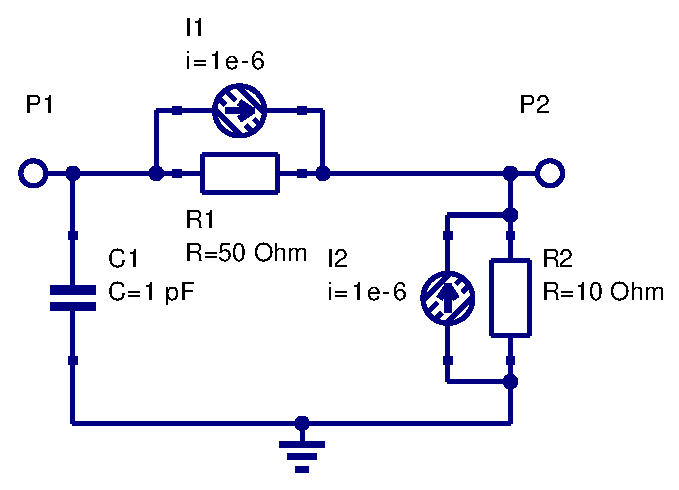
\includegraphics[angle=-90,width=8cm]{CYexample}
\end{center}
\caption{example circuit applied to noise analysis}
\label{fig:CYexample}
\end{figure}
\FloatBarrier

Once having defined the spectral noise current densities of the noise
currents within a transistor model the above rules for forming the
$\underline{C}_Y$ matrix can be applied to the example circuit
depicted in fig. \ref{fig:CYexample}.  The noise current
correlation matrix is accordingly
\begin{equation}
\underline{C}_Y =
\begin{bmatrix}
+\overline{i_1^2} & -\overline{i_1^2}\\
-\overline{i_1^2} & \overline{i_1^2} + \overline{i_2^2}\\
\end{bmatrix}
\end{equation}

\subsection{Transformations}
%\addcontentsline{toc}{subsection}{Transformations}
\label{sec:noiseTrans}

There are three usable noise correlation matrix representations for
multiport circuits.

\begin{itemize}
\item admittance representation $\underline{C}_Y$ - based on noise currents
\item impedance representation $\underline{C}_Z$ - based on noise voltages
\item wave representation $\underline{C}_S$ - based on noise waves
\end{itemize}

According to Scott W. Wedge and David B. Rutledge \cite{Wedge} the
transformations between these representations write as follows.

\begin{center}
\setlength{\fboxsep}{3pt}
\begin{tabular}{|r|c|c|c|}
\hline
&
\setlength{\fboxrule}{0pt}
\fbox{$\underline{C}_Y$}  & $\underline{C}_Z$ & $\underline{C}_S$\\
\hline
$\underline{C}_Y$ & $\underline{C}_Y$ & $Y\cdot \underline{C}_Z\cdot Y^{+}$ &
\setlength{\fboxrule}{0pt}
\fbox{$\left(E + Y\right)\cdot \underline{C}_S\cdot \left(E + Y\right)^{+}$}\\
\hline
$\underline{C}_Z$ & $Z\cdot \underline{C}_Y\cdot Z^{+}$ & $\underline{C}_Z$ &
\setlength{\fboxrule}{0pt}
\fbox{$\left(E + Z\right)\cdot \underline{C}_S\cdot \left(E + Z\right)^{+}$}\\
\hline
$\underline{C}_S$ &
\setlength{\fboxrule}{0pt}
\fbox{$\dfrac{1}{4} \left(E + S\right)\cdot \underline{C}_Y\cdot \left(E + S\right)^{+}$} & $\dfrac{1}{4} \left(E - S\right)\cdot \underline{C}_Z\cdot \left(E - S\right)^{+}$ & $\underline{C}_S$\\
\hline
\end{tabular}
\end{center}

The signal as well as correlation matrices in impedance and admittance
representations are assumed to be normalized in the above table.  $E$
denotes the identity matrix and the $ ^{+}$ operator indicates the
transposed conjugate matrix (also called adjoint or adjugate).

\addvspace{12pt}

Each noise correlation matrix transformation requires the appropriate
signal matrix representation which can be obtained using the formulas
given in section \ref{sec:SparameterConversion} on page
\pageref{sec:SparameterConversion}.

\section{Noise Wave Correlation Matrix of Components}
%\addcontentsline{toc}{section}{Noise Wave Correlation Matrix of Components}

Many components do not produce any noise.  Every element of their
noise correlation matrix therefore equals exactly zero.  Examples are
lossless, passive components, i.e. capacitors, inductors,
transformers, circulators, phase shifters.  Furthermore ideal voltage
and current sources (without internal resistance) as well as gyrators
also do not produce any noise.

\addvspace{12pt}

If one wants to calculate the noise wave correlation matrix of a
component, the most universal method is to take noise voltages and
noise currents and then derive the noise waves by the use of equation
\eqref{equ:waves}.  However, this can be very difficult.

\addvspace{12pt}

A passive, linear circuit produces only thermal noise and thus its
noise waves can be calculated with Bosma's theorem (assuming
thermodynamic equilibrium).

\begin{equation}
(\underline{C}) = k\cdot T\cdot \left( (\underline{E}) - (\underline{S})\cdot(\underline{S})^{*T} \right)
\end{equation}
with $(\underline{S})$ being the S parameter matrix and $(\underline{E})$ identity matrix.
Of course, this theorem can also be written with impedance and admittance representation
of the noise correlation matrix:
\begin{equation}
\underline{C}_Z = 2\cdot k\cdot T\cdot \text{Re}(\underline{Z})
\end{equation}
\begin{equation}
\underline{C}_Y = 2\cdot k\cdot T\cdot \text{Re}(\underline{Y})
\end{equation}


\subsection{Resistor}
%\addcontentsline{toc}{subsection}{Resistor}

Being on temperature $T$, the noise wave correlation matrix of an
ideal, ohmic resistor with resistance $R$ writes as follows.

\begin{equation}
(\underline{C}) = k\cdot T\cdot\frac{4\cdot R\cdot Z_0}{(2\cdot Z_0+R)^2}\cdot
\begin{pmatrix}
   1 & -1\\
  -1 &  1\\
\end{pmatrix}
\end{equation}

The noise wave correlation matrix of a parallel resistor with resistance $R$
writes as follows.

\begin{equation}
(\underline{C}) = k\cdot T\cdot\frac{4\cdot R\cdot Z_0}{(2\cdot R+Z_0)^2}\cdot
\begin{pmatrix}
  1 & 1\\
  1 & 1\\
\end{pmatrix}
\end{equation}

The noise wave correlation matrix of a grounded resistor with resistance $R$
is a matrix consisting of one element and writes as follows.

\begin{equation}
(\underline{C}) = k\cdot T\cdot\frac{4\cdot R\cdot Z_0}{(R+Z_0)^2}
\end{equation}


\subsection{Attenuator}
%\addcontentsline{toc}{subsection}{Attenuator}

Being on temperature $T$, the noise wave correlation matrix of an
ideal attenuator with attenuation $L$ (loss) writes as follows.

\begin{equation}
(\underline{C}) = k\cdot T\cdot\frac{(L-1)\cdot(r^2-1)}{(L-r^2)^2}\cdot
\begin{pmatrix}
  -r^2-L           & 2\cdot r\sqrt{L}\\
  2\cdot r\sqrt{L} & -r^2-L\\
\end{pmatrix}
\end{equation}
with
\begin{equation}
r=\frac{Z_{ref}-Z_0}{Z_{ref}+Z_0}
\end{equation}


\subsection{Isolator}
%\addcontentsline{toc}{subsection}{Isolator}

Being on temperature $T$, the noise wave correlation matrix of an
ideal isolator with reference impedance $Z_1$ and $Z_2$ (input and
output) writes as follows.

\begin{equation}
(\underline{C}) = \frac{4\cdot k\cdot T\cdot Z_0}{(Z_1+Z_0)^2}\cdot
\begin{pmatrix}
  Z_1           & \sqrt{Z_1\cdot Z_2}\cdot\frac{Z_0-Z_1}{Z_0+Z_2}\\
  \sqrt{Z_1\cdot Z_2}\cdot\frac{Z_0-Z_1}{Z_0+Z_2} & Z_2\cdot\left(\frac{Z_1-Z_0}{Z_2+Z_0}\right)^2\\
\end{pmatrix}
\end{equation}


\subsection{Noise sources}
%\addcontentsline{toc}{subsection}{Noise sources}

The noise wave correlation matrix of a noise voltage source with
voltage power spectral density $vPSD$ writes as follows.

\begin{equation}
(\underline{C}) = \frac{vPSD}{4\cdot Z_0}\cdot
\begin{pmatrix}
   1 & -1\\
  -1 &  1\\
\end{pmatrix}
\end{equation}

The noise wave correlation matrix of a noise current source with
current power spectral density $cPSD$ writes as follows.

\begin{equation}
(\underline{C}) = cPSD\cdot Z_0\cdot
\begin{pmatrix}
   1 & -1\\
  -1 &  1\\
\end{pmatrix}
\end{equation}

To implement the frequency dependencies of all common PSDs the
following equation can be used.

\begin{equation}
PSD = \frac{PSD_0}{a+b\cdot f^c}
\end{equation}

Where $f$ is frequency and $a$, $b$, $c$ are the parameters.  The
following PSDs appear in electric devices.

\addvspace{12pt}

\begin{tabular}{ll}
white noise (thermal noise, shot noise):         & $a=0$, $b=1$, $c=0$ \\
pink noise (flicker noise):                      & $a=0$, $b=1$, $c=1$ \\
Lorentzian PSD (generation-recombination noise): & $a=1$, $b=1/f_c^2$, $c=2$ \\
\end{tabular}


\subsection{Diode}
%\addcontentsline{toc}{subsection}{Diode}
\label{sec:nw_diode}

An ideal diode (pn- or schottky-diode) generates shot noise.  Both
types of current (field and diffusion) contribute independently to it.
That is, even though the two currents flow in different directions
("minus" in dc current equation), they have to be added in the noise
equation (current is proportional to noise power spectral density).
Taking into account the dynamic conductance $g_d$ in parallel to the
noise current source, the noise wave correlation matrix writes as
follows.

\begin{equation}
\begin{split}
(\underline{C})
 =  \left| \frac{0.5\cdot Y_0}{g_d+j\omega C_d + 0.5\cdot Y_0}\right|^2  \cdot 2\cdot e\cdot I_S\cdot
    \left( \exp\left( \frac{V_{d}}{N\cdot V_T} \right) +1 \right) \cdot Z_0\cdot\begin{pmatrix}
   1 & -1\\
  -1 &  1\\
\end{pmatrix} \\
 = 2\cdot e\cdot Z_0\cdot \left(I_{d} + 2\cdot I_{S}\right)\cdot
    \left| \frac{1}{2\cdot Z_0\cdot (g_d+j\omega C_d) + 1}\right|^2 \cdot
\begin{pmatrix}
   1 & -1\\
  -1 &  1\\
\end{pmatrix}
\end{split}
\end{equation}

Where $e$ is charge of an electron, $V_T$ the temperature voltage,
$g_d$ the (dynamic) conductance of the diode and $C_d$ its junction
capacitance.

\addvspace{12pt}

To be very precise, the equation above only holds for diodes whose
field and diffusion current dominate absolutely (diffusion limited
diode), i.e. $N=1$.  Many diodes also generate a
generation/recombination current ($N\approx 2$), which produces shot
noise, too.  But depending on where and how the charge carriers
generate or recombine, their effective charge is somewhat smaller than
$e$.  To take this into account, one needs a further factor $K$.
Several opinions exist according the value of $K$.  Some say 1 and 2/3
are common values, others say $K=1/N$ with $K$ and $N$ being bias
dependent.  Altogether it is:
\begin{equation}
\begin{split}
(\underline{C})
 = 2\cdot e\cdot Z_0\cdot K\cdot \left(I_{d} + 2\cdot I_{S}\right)\cdot
    \left| \frac{1}{2\cdot Z_0\cdot (g_d+j\omega C_d) + 1}\right|^2 \cdot
\begin{pmatrix}
   1 & -1\\
  -1 &  1\\
\end{pmatrix}\\
\text{with}\qquad\frac{1}{2}\le K \le 1
\end{split}
\label{eq:diode_noise}
\end{equation}

Remark: Believing the diode equation $I_D = I_S\cdot (\exp(V/(N\cdot
V_T)) - 1)$ is the whole truth, it is logical to define $K=1/N$,
because at $V=0$ the conductance $g_d$ of the diode must create
thermal noise.

\addvspace{12pt}

Some special diodes have additional current or noise components
(tunnel diodes, avalanche diodes etc.).  All these mechanisms are not
taken into account in equation \eqref{eq:diode_noise}.

\addvspace{12pt}

The parasitic ohmic resistance in a non-ideal diode, of course,
creates thermal noise.

\subsection{S-parameter container with additional reference port}
%\addcontentsline{toc}{subsection}{S-parameter container with additional reference port}

\begin{figure}[ht]
\begin{center}
\includegraphics[width=0.6\linewidth]{spnfile}
\end{center}
\caption{S-parameter container with noise wave correlation matrix}
\label{fig:spnfile}
\end{figure}
\FloatBarrier

With the S-parameter transformation done, as noted in section
\ref{sec:spfile} on page \pageref{sec:spfile}, the $m$-port noise wave
correlation matrix is
\begin{equation}
C_m = \left|\dfrac{1}{1 - \Gamma_m}\right|^2 \cdot \left(K\cdot C_{m-1}\cdot K^+ -T_s\cdot k_B \cdot\left|1 - \left|\Gamma_m\right|^2\right|\cdot D\cdot D^+\right)
\end{equation}

with
\begin{align}
K &=
\begin{bmatrix}
1 + \Gamma_m\left(S_{1m} -1\right) & \Gamma_m S_{1m} & \ldots & \Gamma_m S_{1m}\\
\Gamma_m S_{2m} & 1 + \Gamma_m\left(S_{2m} -1\right) & \ldots & \Gamma_m S_{2m}\\
\vdots & \vdots & \ddots & \vdots\\
\Gamma_m S_{(m-1)m} & \Gamma_m S_{(m-1)m} & \ldots & 1 + \Gamma_m\left(S_{(m-1)m} -1\right)\\
\Gamma_m S_{mm} - 1 & \Gamma_m S_{mm} - 1 & \ldots & \Gamma_m S_{mm} - 1
\end{bmatrix}\\
D &=
\begin{bmatrix}
S_{1m}\\
S_{2m}\\
\vdots\\
S_{(m-1)m}\\
S_{mm} - 1
\end{bmatrix}
\end{align}

whence $T_s$ denotes the equivalent noise temperature of the original
reference port and the $ ^{+}$ operator indicates the transposed
conjugate matrix (also called adjoint or adjugate).

\addvspace{12pt}

The reverse transformation can be written as
\begin{equation}
C_{m-1} = K'\cdot C_m\cdot K'^+ +T_s\cdot k_B \cdot\dfrac{\left|1 - \left|\Gamma_m\right|^2\right|}{\left|1 - \Gamma_m S_{mm}\right|^2}\cdot D'\cdot D'^+
\end{equation}

with
\begin{align}
K' &=
\begin{bmatrix}
1 & 0 & \ldots & 0 & \dfrac{\Gamma_m S_{1m}}{1 - \Gamma_m S_{mm}}\\
0 & 1 & \ldots & 0 & \dfrac{\Gamma_m S_{2m}}{1 - \Gamma_m S_{mm}}\\
. & . & \ddots & . & \vdots\\
0 & 0 & \ldots & 1 & \dfrac{\Gamma_m S_{(m-1)m}}{1 - \Gamma_m S_{mm}}\\
\end{bmatrix}\\
D' &=
\begin{bmatrix}
S_{1m}\\
S_{2m}\\
\vdots\\
S_{(m-1)m}
\end{bmatrix}
\end{align}


%
% This document contains the chapter about DC analysis.
%
% Copyright (C) 2003, 2004 Stefan Jahn <stefan@lkcc.org>
% Copyright (C) 2004 Michael Margraf <Michael.Margraf@alumni.TU-Berlin.DE>
%
% Permission is granted to copy, distribute and/or modify this document
% under the terms of the GNU Free Documentation License, Version 1.1
% or any later version published by the Free Software Foundation.
%

\chapter{DC Analysis}
%\addcontentsline{toc}{chapter}{DC Analysis}

\section{Modified Nodal Analysis}
%\addcontentsline{toc}{section}{Modified Nodal Analysis}
\label{sec:MNA}

Many different kinds of network element are encountered in network
analysis.  For circuit analysis it is necessary to formulate equations
for circuits containing as many different types of network elements as
possible.  There are various methods for equation formulation for a
circuit.  These are based on three types of equations found in circuit
theory:

\begin{itemize}
\item equations based on Kirchhoff's voltage law (KVL)
\item equations based on Kirchhoff's current law (KCL)
\item branch constitutive equations
\end{itemize}

The equations have to be formulated (represented in a computer
program) automatically in a simple, comprehensive manner.  Once
formulated, the system of equations has to be solved.  There are two
main aspects to be considered when choosing algorithms for this
purpose: accuracy and speed.  The MNA, briefly for \textbf{M}odified
\textbf{N}odal \textbf{A}nalysis, has been proved to accomplish these
tasks.

MNA applied to a circuit with passive elements, independent current
and voltage sources and active elements results in a matrix equation
of the form:
\begin{equation}
\left[A\right] \cdot \left[x\right] = \left[z\right]
\end{equation}

For a circuit with N nodes and M independent voltage sources:

\begin{itemize}

\item The A matrix
\begin{itemize}
\item
is (N+M)$\times$(N+M) in size, and consists only of known quantities
\item
the N$\times$N part of the matrix in the upper left:
\begin{itemize}
\item
has only passive elements
\item
elements connected to ground appear only on the diagonal
\item
elements not connected to ground are both on the diagonal and
off-diagonal terms
\end{itemize}
\item
the rest of the A matrix (not included in the N$\times$N upper left
part) contains only 1, -1 and 0 (other values are possible if there
are dependent current and voltage sources)
\end{itemize}

\item The x matrix
\begin{itemize}
\item
is an (N+M)$\times$1 vector that holds the unknown quantities (node
voltages and the currents through the independent voltage sources)
\item
the top N elements are the n node voltages
\item
the bottom M elements represent the currents through the M independent
voltage sources in the circuit
\end{itemize}

\item The z matrix
\begin{itemize}
\item
is an (N+M)$\times$1 vector that holds only known quantities
\item
the top N elements are either zero or the sum and difference of
independent current sources in the circuit
\item
the bottom M elements represent the M independent voltage sources in
the circuit
\end{itemize}
\end{itemize}

The circuit is solved by a simple matrix manipulation:
\begin{equation}
\left[x\right] = \left[A\right]^{-1} \cdot \left[z\right]
\end{equation}

Though this may be difficult by hand, it is straightforward and so is
easily done by computer.

\subsection{Generating the MNA matrices}
%\addcontentsline{toc}{subsection}{Generating the MNA matrices}

The following section is an algorithmic approach to the concept of the
Modified Nodal Analysis.  There are three matrices we need to
generate, the A matrix, the x matrix and the z matrix.  Each of these
will be created by combining several individual sub-matrices.

\subsection{The A matrix}
%\addcontentsline{toc}{subsection}{The A matrix}

The A matrix will be developed as the combination of 4 smaller
matrices, G, B, C, and D.

\begin{equation}
A =
\begin{bmatrix}
G & B\\
C & D
\end{bmatrix}
\end{equation}

The A matrix is (M+N)$\times$(M+N) (N is the number of nodes, and M is the
number of independent voltage sources) and:

\begin{itemize}
\item
the G matrix is N$\times$N and is determined by the interconnections
between the circuit elements
\item
the B matrix is M$\times$N and is determined by the connection of the voltage
sources
\item
the C matrix is N$\times$M and is determined by the connection of
the voltage sources (B and C are closely related, particularly when
only independent sources are considered)
\item
the D matrix is M$\times$M and is zero if only independent sources are
considered
\end{itemize}

\subsubsection{Rules for making the G matrix}
%\addcontentsline{toc}{subsubsection}{Rules for making the G matrix}

The G matrix is an N$\times$N matrix formed in two steps.

\begin{enumerate}
\item
Each element in the diagonal matrix is equal to the sum of the
conductance (one over the resistance) of each element connected to the
corresponding node.  So the first diagonal element is the sum of
conductances connected to node 1, the second diagonal element is the
sum of conductances connected to node 2, and so on.
\item
The off diagonal elements are the negative conductance of the element
connected to the pair of corresponding node.  Therefore a resistor
between nodes 1 and 2 goes into the G matrix at location (1,2) and
locations (2,1).
\end{enumerate}

If an element is grounded, it will only have contribute to one entry
in the G matrix -- at the appropriate location on the diagonal.  If it
is ungrounded it will contribute to four entries in the matrix -- two
diagonal entries (corresponding to the two nodes) and two off-diagonal
entries.

\subsubsection{Rules for making the B matrix}
%\addcontentsline{toc}{subsubsection}{Rules for making the B matrix}

The B matrix is an M$\times$N matrix with only 0, 1 and -1 elements.
Each location in the matrix corresponds to a particular voltage source
(first dimension) or a node (second dimension).  If the positive
terminal of the ith voltage source is connected to node k, then the
element (i,k) in the B matrix is a 1.  If the negative terminal of the
ith voltage source is connected to node k, then the element (i,k) in
the B matrix is a -1.  Otherwise, elements of the B matrix are zero.

\addvspace{12pt}

If a voltage source is ungrounded, it will have two elements in the B
matrix (a 1 and a -1 in the same column).  If it is grounded it will
only have one element in the matrix.

\subsubsection{Rules for making the C matrix}
%\addcontentsline{toc}{subsubsection}{Rules for making the C matrix}

The C matrix is an N$\times$M matrix with only 0, 1 and -1 elements.
Each location in the matrix corresponds to a particular node (first
dimension) or voltage source (second dimension).  If the positive
terminal of the ith voltage source is connected to node k, then the
element (k,i) in the C matrix is a 1.  If the negative terminal of the
ith voltage source is connected to node k, then the element (k,i) in
the C matrix is a -1.  Otherwise, elements of the C matrix are zero.

\addvspace{12pt}

In other words, the C matrix is the transpose of the B matrix.  This
is not the case when dependent sources are present.

\subsubsection{Rules for making the D matrix}
%\addcontentsline{toc}{subsubsection}{Rules for making the D matrix}

The D matrix is an M$\times$M matrix that is composed entirely of
zeros.  It can be non-zero if dependent sources are considered.

\subsection{The x matrix}
\label{sec:xmatrix}
%\addcontentsline{toc}{subsection}{The x matrix}

The x matrix holds our unknown quantities and will be developed as the
combination of 2 smaller matrices v and j.  It is considerably easier
to define than the A matrix.

\begin{equation}
x =
\begin{bmatrix}
v\\
j
\end{bmatrix}
\end{equation}

The x matrix is 1$\times$(M+N) (N is the number of nodes, and M is the
number of independent voltage sources) and:

\begin{itemize}
\item
the v matrix is 1$\times$N and hold the unknown voltages
\item
the j matrix is 1$\times$M and holds the unknown currents through the
voltage sources
\end{itemize}

\subsubsection{Rules for making the v matrix}
%\addcontentsline{toc}{subsubsection}{Rules for making the v matrix}

The v matrix is an 1$\times$N matrix formed of the node voltages.
Each element in v corresponds to the voltage at the equivalent node in
the circuit (there is no entry for ground -- node 0).

\addvspace{12pt}

For a circuit with N nodes we get:

\begin{equation}
v =
\begin{bmatrix}
v_{1}\\
v_{2}\\
\vdots\\
v_{N}\\
\end{bmatrix}
\end{equation}

\subsubsection{Rules for making the j matrix}
%\addcontentsline{toc}{subsubsection}{Rules for making the j matrix}

The j matrix is an 1$\times$M matrix, with one entry for the current
through each voltage source.  So if there are M voltage sources
$V_{1}$, $V_{2}$ through $V_{M}$, the j matrix will be:

\begin{equation}
j =
\begin{bmatrix}
i_{V_{1}}\\
i_{V_{2}}\\
\vdots\\
i_{V_{M}}\\
\end{bmatrix}
\end{equation}

\subsection{The z matrix}
%\addcontentsline{toc}{subsection}{The z matrix}

The z matrix holds our independent voltage and current sources and
will be developed as the combination of 2 smaller matrices i and e.
It is quite easy to formulate.

\begin{equation}
z =
\begin{bmatrix}
i\\
e
\end{bmatrix}
\end{equation}

The z matrix is 1$\times$(M+N) (N is the number of nodes, and M is the
number of independent voltage sources) and:

\begin{itemize}
\item
the i matrix is 1$\times$N and contains the sum of the currents through the
passive elements into the corresponding node (either zero, or the sum
of independent current sources)
\item
the e matrix is 1$\times$M and holds the values of the independent
voltage sources
\end{itemize}

\subsubsection{Rules for making the i matrix}
%\addcontentsline{toc}{subsubsection}{Rules for making the i matrix}

The i matrix is an 1$\times$N matrix with each element of the matrix
corresponding to a particular node.  The value of each element of i is
determined by the sum of current sources into the corresponding node.
If there are no current sources connected to the node, the value is
zero.

\subsubsection{Rules for making the e matrix}
%\addcontentsline{toc}{subsubsection}{Rules for making the e matrix}

The e matrix is an 1$\times$M matrix with each element of the matrix
equal in value to the corresponding independent voltage source.

\subsection{A simple example}
%\addcontentsline{toc}{subsection}{A simple example}

The example given in fig. \ref{fig:MNAexample} illustrates applying
the rules for building the MNA matrices and how this relates to basic
equations used in circuit analysis.

\begin{figure}[ht]
\begin{center}
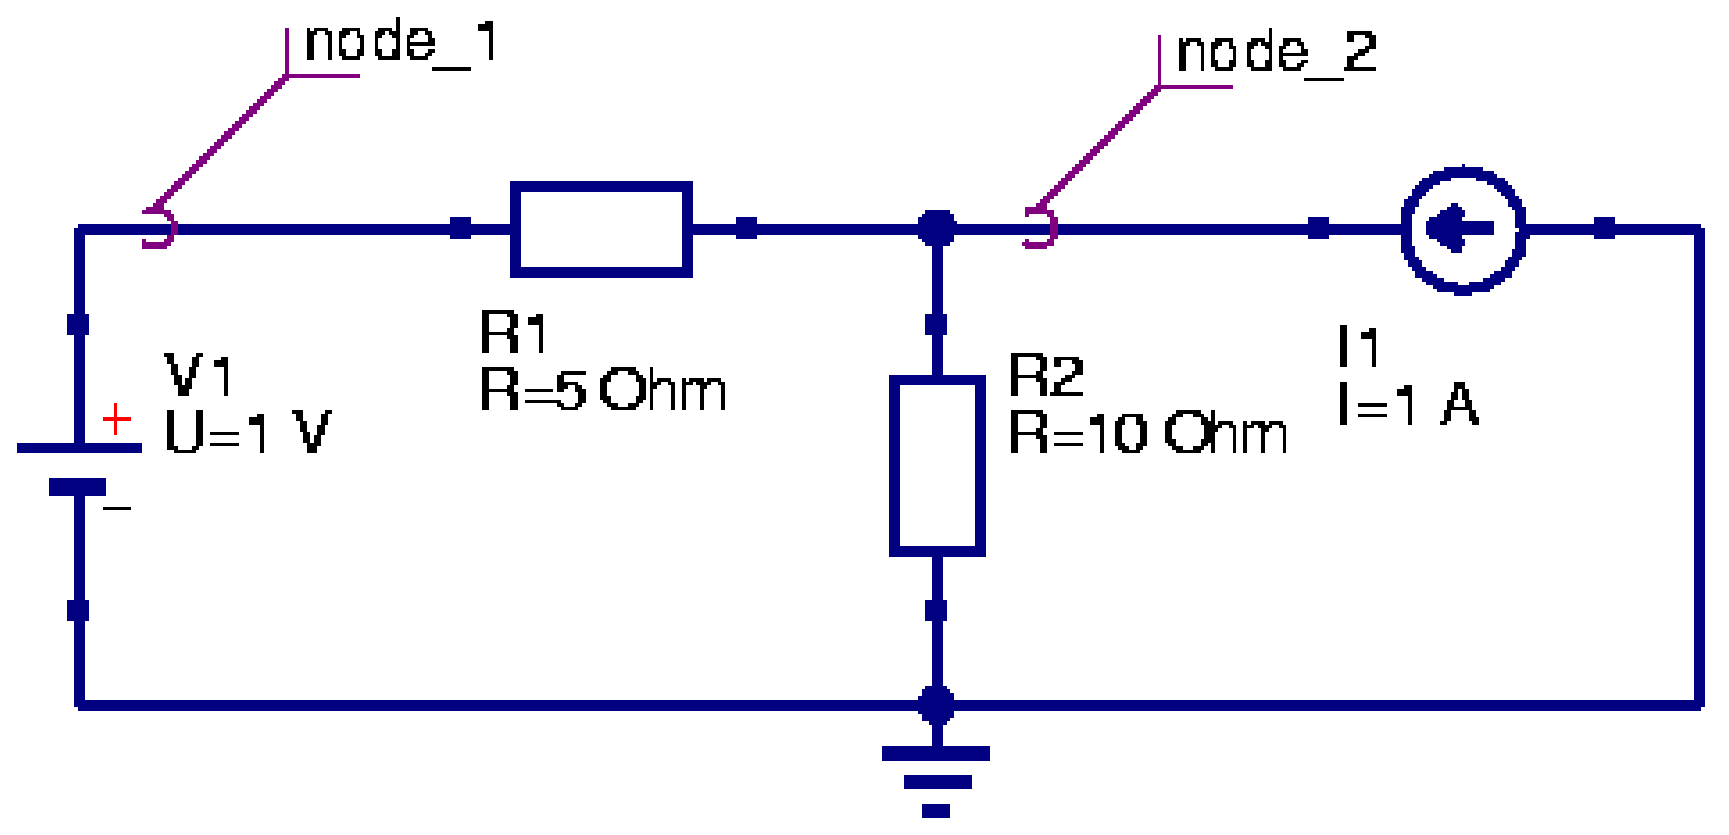
\includegraphics[width=10cm]{MNAexample}
\end{center}
\caption{example circuit applied to modified nodal analysis}
\label{fig:MNAexample}
\end{figure}
\FloatBarrier

\subsubsection{Going through the MNA algorithm}
%\addcontentsline{toc}{subsubsection}{Going through the MNA algorithm}

The G matrix is a 2$\times$2 matrix because there are 2 different
nodes apart from ground which is the reference node.  On the diagonal
you find the sum of the elements conductances connected to the nodes 1
and 2.  The off-diagonal matrix entries contain the negative
conductances of the elements connected between two nodes.

\begin{equation}
G =
\begin{bmatrix}
\frac{1}{R_{1}} & -\frac{1}{R_{1}}\\
-\frac{1}{R_{1}} & \frac{1}{R_{1}} + \frac{1}{R_{2}}
\end{bmatrix}
=
\begin{bmatrix}
0.2 & -0.2\\
-0.2 & 0.3
\end{bmatrix}
\end{equation}

The B matrix (which is transposed to C) is a 1$\times$2 matrix because
there is one voltage source and 2 nodes.  The positive terminal of the
voltage source $V_{1}$ is connected to node 1.  That is why

\begin{equation}
B = C^{T} =
\begin{bmatrix}
1\\
0
\end{bmatrix}
\end{equation}

and the D matrix is filled with zeros only because there are no dependent
(active and controlled) devices in the example circuit.

\begin{equation}
D =
\begin{bmatrix}
0
\end{bmatrix}
\end{equation}

The x matrix is a 1$\times$3 matrix.  The MNA equations deliver a
solution for the unknown voltages at each node in a circuit except the
reference node and the currents through each voltage source.

\begin{equation}
x =
\begin{bmatrix}
v_{1}\\
v_{2}\\
i_{V_{1}}
\end{bmatrix}
\end{equation}

The z matrix is according to the rules for building it a 1$\times$3
matrix.  The upper two entries are the sums of the currents flowing
into node 1 and node 2.  The lower entry is the voltage value of the
voltage source $V_{1}$.

\begin{equation}
z =
\begin{bmatrix}
0\\
I_{1}\\
U_{1}
\end{bmatrix}
=
\begin{bmatrix}
0\\
1\\
1
\end{bmatrix}
\end{equation}

According to the MNA algorithm the equation system is represented by

\begin{equation}
\left[A\right] \cdot \left[x\right] = \left[z\right]
\end{equation}

which is equivalent to

\begin{equation}
\begin{bmatrix}
G & B\\
C & D
\end{bmatrix}
\cdot
\begin{bmatrix}
x
\end{bmatrix}
=
\begin{bmatrix}
z
\end{bmatrix}
\label{eq:MNAexample}
\end{equation}

In the example eq. \eqref{eq:MNAexample} expands to:

\begin{equation}
\begin{bmatrix}
\frac{1}{R_{1}} & -\frac{1}{R_{1}} & 1\\
-\frac{1}{R_{1}} & \frac{1}{R_{1}} + \frac{1}{R_{2}} & 0\\
1 & 0 & 0
\end{bmatrix}
\cdot
\begin{bmatrix}
v_{1}\\
v_{2}\\
i_{V_{1}}
\end{bmatrix}
=
\begin{bmatrix}
0\\
I_{1}\\
U_{1}
\end{bmatrix}
\label{eq:MNAfull}
\end{equation}

The equation systems to be solved is now defined by the following
matrix representation.

\begin{equation}
\begin{bmatrix}
0.2 & -0.2 & 1\\
-0.2 & 0.3 & 0\\
1 & 0 & 0
\end{bmatrix}
\cdot
\begin{bmatrix}
v_{1}\\
v_{2}\\
i_{V_{1}}
\end{bmatrix}
=
\begin{bmatrix}
0\\
1\\
1
\end{bmatrix}
\end{equation}

Using matrix inversion the solution vector x writes as follows:

\begin{equation}
\left[x\right] = 
\left[A\right]^{-1}\cdot \left[z\right] = 
\begin{bmatrix}
v_{1}\\
v_{2}\\
i_{V_{1}}
\end{bmatrix}
=
\begin{bmatrix}
1\\
4\\
0.6
\end{bmatrix}
\label{eq:MNAresult}
\end{equation}

The result in eq. (\ref{eq:MNAresult}) denotes the current through the
voltage source $V_{1}$ is $0.6\ampere$, the voltage at node 1 is
$1\volt$ and the voltage at node 2 is $4\volt$.

\subsubsection{How the algorithm relates to basic equations in circuit analysis}
%\addcontentsline{toc}{subsubsection}{How the algorithm relates to basic equations in circuit analysis}

Expanding the matrix representation in eq. (\ref{eq:MNAfull}) to a set
of equations denotes the following equation system consisting of 3 of
them.

\begin{align}
\rm{I:}& \qquad 0 = \frac{1}{R_{1}}\cdot v_{1} - \frac{1}{R_{1}}\cdot v_{2} + i_{V_{1}}& \text{KCL at node 1}\\
\rm{II:}& \qquad I_{1} = -\frac{1}{R_{1}}\cdot v_{1} + \left(\frac{1}{R_{1}} + \frac{1}{R_{2}}\right)\cdot v_{2}& \text{KCL at node 2}\\
\rm{III:}& \qquad U_{1} = v_{1}& \text{constitutive equation}
\end{align}

Apparently eq. I and eq. II conform to Kirchhoff's current law at the
nodes 1 and 2.  The last equation is just the constitutive equation
for the voltage source $V_{1}$.  There are three unknowns ($v_{1}$,
$v_{2}$ and $i_{V_{1}}$) and three equations, thus the system should
be solvable.

\addvspace{12pt}

Equation III indicates the voltage at node 1 is $1\volt$.  Applying
this result to eq. II and transposing it to $v_{2}$ (the voltage at
node 2) gives

\begin{equation}
v_{2} = \frac{I_{1} + \frac{1}{R_{1}}\cdot U_{1}}{\frac{1}{R_{1}} + \frac{1}{R_{2}}} = 4\volt
\end{equation}

The missing current through the voltage source $V_{1}$ can be computed
using both the results $v_{2} = 4\volt$ and $v_{1} = 1\volt$ by
transforming equation I.

\begin{equation}
i_{V_{1}} = \frac{1}{R_{1}}\cdot v_{2} - \frac{1}{R_{1}}\cdot v_{1} = 0.6\ampere
\end{equation}

The small example, shown in fig. \ref{fig:MNAexample}, and the
excursus into artless math verifies that the MNA algorithm and classic
electrical handiwork tend to produce the same results.

\section{Solving linear equation systems}
%\addcontentsline{toc}{section}{Solving linear equation systems}

When dealing with non-linear networks the number of equation systems
to be solved depends on the required precision of the solution and the
average necessary iterations until the solution is stable.  This
emphasizes the meaning of the solving procedures choice for different
problems.

\addvspace{12pt}

The equation systems
\begin{equation}
\left[A\right] \cdot \left[x\right] = \left[z\right]
\end{equation}
solution can be written as
\begin{equation}
\left[x\right] = \left[A\right]^{-1} \cdot \left[z\right]
\end{equation}

\subsection{Matrix inversion}
%\addcontentsline{toc}{subsection}{Matrix inversion}

The elements $\beta_{\mu\nu}$ of the inverse of the matrix $A$ are
\begin{equation}
\beta_{\mu\nu} = \frac{A_{\mu\nu}}{det A}
\end{equation}
whereas $A_{\mu\nu}$ is the matrix elements $a_{\mu\nu}$ cofactor.
The cofactor is the sub determinant (i.e. the minor) of the element
$a_{\mu\nu}$ multiplied with $(-1)^{\mu + \nu}$.  The determinant of a
square matrix can be recursively computed by either of the following
equations.
\begin{align}
det A = \sum_{\mu = 1}^{n} a_{\mu\nu}\cdot A_{\mu\nu}
\quad &\text{using the $\nu$-th column}\\
det A = \sum_{\nu = 1}^{n} a_{\mu\nu}\cdot A_{\mu\nu}
\quad &\text{using the $\mu$-th row}
\end{align}

This method is called the Laplace expansion.  In order to save
computing time the row or column with the most zeros in it is used for
the expansion expressed in the above equations.  A sub determinant
$(n-1)$-th order of a matrix's element $a_{\mu\nu}$ of $n$-th order is
the determinant which is computed by canceling the $\mu$-th row and
$\nu$-th column.  The following example demonstrates calculating the
determinant of a 4th order matrix with the elements of the 3rd row.
\begin{align}
\begin{vmatrix}
a_{11} & a_{12} & a_{13} & a_{14}\\
a_{21} & a_{22} & a_{23} & a_{24}\\
a_{31} & a_{32} & a_{33} & a_{34}\\
a_{41} & a_{42} & a_{43} & a_{44}\\
\end{vmatrix}
&= a_{31}
\begin{vmatrix}
a_{12} & a_{13} & a_{14}\\
a_{22} & a_{23} & a_{24}\\
a_{42} & a_{43} & a_{44}\\
\end{vmatrix}
- a_{32}
\begin{vmatrix}
a_{11} & a_{13} & a_{14}\\
a_{21} & a_{23} & a_{24}\\
a_{41} & a_{43} & a_{44}\\
\end{vmatrix}\\
\nonumber
&+ a_{33}
\begin{vmatrix}
a_{11} & a_{12} & a_{14}\\
a_{21} & a_{22} & a_{24}\\
a_{41} & a_{42} & a_{44}\\
\end{vmatrix}
- a_{34}
\begin{vmatrix}
a_{11} & a_{12} & a_{13}\\
a_{21} & a_{22} & a_{23}\\
a_{41} & a_{42} & a_{43}\\
\end{vmatrix}
\end{align}

This recursive process for computing the inverse of a matrix is most
easiest to be implemented but as well the slowest algorithm.  It
requires approximately $n!$ operations.

\subsection{Gaussian elimination}
%\addcontentsline{toc}{subsection}{Gaussian elimination}

The Gaussian algorithm for solving a linear equation system is done in
two parts: forward elimination and backward substitution.  During
forward elimination the matrix A is transformed into an upper
triangular equivalent matrix.  Elementary transformations due to an
equation system having the same solutions for the unknowns as the
original system.

\begin{equation}
A =
\begin{bmatrix}
a_{11} & a_{12} & \ldots & a_{1n}\\
a_{21} & a_{22} & \ldots & a_{2n}\\
\vdots & \vdots & \ddots & \vdots\\
a_{n1} & a_{n2} & \ldots & a_{nn}
\end{bmatrix}
\rightarrow
\begin{bmatrix}
a_{11} & a_{12} & \ldots & a_{1n}\\
0 & a_{22} & \ldots & a_{2n}\\
\vdots & \vdots & \ddots & \vdots\\
0 & \ldots & 0 & a_{nn}
\end{bmatrix}
\end{equation}

The modifications applied to the matrix A in order to achieve this
transformations are limited to the following set of operations.
\begin{itemize}
\item multiplication of a row with a scalar factor
\item addition or subtraction of multiples of rows
\item exchanging two rows of a matrix
\end{itemize}

\subsubsection{Step 1: Forward elimination}
%\addcontentsline{toc}{subsubsection}{Step 1: Forward elimination}

The transformation of the matrix A is done in $\mathrm{n - 1}$
elimination steps.  The new matrix elements of the k-th step with
$\mathrm{k = 1, \ldots, n - 1}$ are computed with the following
recursive formulas.

\begin{align}
a_{ij} &= 0 & i = k+1, \ldots, n &\text{ and } j = k\\
a_{ij} &= a_{ij} - a_{kj} \cdot a_{ik} / a_{kk} & i = k+1, \ldots, n &\text{ and } j = k+1, \ldots, n\\
z_{i} &= z_{i} - z_{k} \cdot a_{ik} / a_{kk} & i = k+1, \ldots, n &
\end{align}

The triangulated matrix can be used to calculate the determinant very
easily.  The determinant of a triangulated matrix is the product of
the diagonal elements.  If the determinant $det A$ is non-zero the
equation system has a solution.  Otherwise the matrix A is singular.

\begin{equation}
det A = a_{11}\cdot a_{22}\cdot \ldots \cdot a_{nn} = \prod_{i=1}^{n} a_{ii}
\end{equation}

When using row and/or column pivoting the resulting determinant may
differ in its sign and must be multiplied with $(-1)^m$ whereas $m$ is
the number of row and column substitutions.

\subsubsection{Finding an appropriate pivot element}
%\addcontentsline{toc}{subsubsection}{Finding an appropriate pivot element}

The Gaussian elimination fails if the pivot element $a_{kk}$ turns to
be zero (division by zero).  That is why row and/or column pivoting
must be used before each elimination step.  If a diagonal element
$a_{kk} = 0$, then exchange the pivot row $k$ with the row $m > k$
having the coefficient with the largest absolute value.  The new pivot
row is $m$ and the new pivot element is going to be $a_{mk}$.  If no
such pivot row can be found the matrix is singular.

\addvspace{12pt}

Total pivoting looks for the element with the largest absolute value
within the matrix and exchanges rows and columns.  When exchanging
columns in equation systems the unknowns get reordered as well.  For
the numerical solution of equation systems with Gaussian elimination
column pivoting is clever, and total pivoting recommended.

\addvspace{12pt}

In order to improve numerical stability pivoting should also be
applied if $a_{kk} \ne 0$ because division by small diagonal elements
propagates numerical (rounding) errors.  This appears especially with
poorly conditioned (the two dimensional case: two lines with nearly
the same slope) equation systems.

\subsubsection{Step 2: Backward substitution}
%\addcontentsline{toc}{subsubsection}{Step 2: Backward substitution}

The solutions in the vector x are obtained by backward substituting
into the triangulated matrix.  The elements of the solution vector x
are computed by the following recursive equations.

\begin{align}
x_{n} &= \frac{z_{n}}{a_{nn}}\\
x_{i} &= \frac{z_{i}}{a_{ii}} - \sum_{k=i+1}^{n} x_{k}\cdot \frac{a_{ik}}{a_{ii}} & i = n - 1,\ldots,1
\end{align}

The forward elimination in the Gaussian algorithm requires
approximately $n^3/3$, the backward substitution $n^2/2$ operations.

\subsection{Gauss-Jordan method}
%\addcontentsline{toc}{subsection}{Gauss-Jordan method}

The Gauss-Jordan method is a modification of the Gaussian elimination.
In each k-th elimination step the elements of the k-th column get zero
except the diagonal element which gets 1.  When the right hand side
vector z is included in each step it contains the solution vector x
afterwards.

\addvspace{12pt}

The following recursive formulas must be applied to get the new matrix
elements for the k-th elimination step.  The k-th row must be computed
first.
\begin{align}
a_{kj} &= a_{kj} / a_{kk} & j = 1\ldots n\\
z_{k}  &= z_{k} / a_{kk}  &
\end{align}

Then the other rows can be calculated with the following formulas.
\begin{align}
a_{ij} &= a_{ij} - a_{ik}\cdot a_{kj} & j = 1,\ldots,n \textrm{ and } i = 1,\ldots,n \textrm{ with } i \ne k\\
z_{i}  &= z_{i} - a_{ik}\cdot z_{k}   & i = 1,\ldots,n \textrm{ with } i \ne k
\end{align}

Column pivoting may be necessary in order to avoid division by zero.
The solution vector x is not harmed by row substitutions.  When the
Gauss-Jordan algorithm has been finished the original matrix has been
transformed into the identity matrix.  If each operation during this
process is applied to an identity matrix the resulting matrix is the
inverse matrix of the original matrix.  This means that the
Gauss-Jordan method can be used to compute the inverse of a matrix.

\addvspace{12pt}

Though this elimination method is easy to implement the number of
required operations is larger than within the Gaussian elimination.
The Gauss-Jordan method requires approximately $N^3/2 + N^2/2$
operations.

\subsection{LU decomposition}
%\addcontentsline{toc}{subsection}{LU decomposition}

LU decomposition (decomposition into a lower and upper triangular
matrix) is recommended when dealing with equation systems where the
matrix A does not alter but the right hand side (the vector z) does.
Both the Gaussian elimination and the Gauss-Jordan method involve both
the right hand side and the matrix in their algorithm.  Consecutive
solutions of an equation system with an altering right hand side can
be computed faster with LU decomposition.

\addvspace{12pt}

The LU decomposition splits a matrix A into a product of a lower
triangular matrix L with an upper triangular matrix U.

\begin{equation}
A = L U \;\text{ with }\;
L = 
\begin{bmatrix}
l_{11} & 0 & \ldots & 0\\
l_{21} & l_{22} & \ddots & \vdots\\
\vdots &  & \ddots & 0\\
l_{n1} & \ldots & \ldots & l_{nn}
\end{bmatrix}
\;\text{ and }\;
U =
\begin{bmatrix}
u_{11} & u_{12} & \ldots & u_{1n}\\
0 & u_{22} &  & \vdots\\
\vdots & \ddots & \ddots & \vdots\\
0 & \ldots & 0 & u_{nn}
\end{bmatrix}
\end{equation}

The algorithm for solving the linear equation system $Ax = z$ involves
three steps:
\begin{itemize}
\item LU decomposition of the coefficient matrix A\\
$\rightarrow Ax = LUx = z$
\item introduction of an (unknown) arbitrary vector y and solving the equation system $Ly = z$ by forward substitution\\
$\rightarrow y = Ux = L^{-1}z$
\item solving the equation system $Ux = y$  by backward substitution\\
$\rightarrow x = U^{-1}y$
\end{itemize}

The decomposition of the matrix A into a lower and upper triangular
matrix is not unique.  The most important decompositions, based on
Gaussian elimination, are the Doolittle, the Crout and the Cholesky
decomposition.

\addvspace{12pt}

If pivoting is necessary during these algorithms they do not decompose
the matrix $A$ but the product with an arbitrary matrix $PA$ (a
permutation of the matrix $A$).  When exchanging rows and columns the
order of the unknowns as represented by the vector $z$ changes as well
and must be saved during this process for the forward substitution in
the algorithms second step.

\subsubsection{Step 1: LU decomposition}
%\addcontentsline{toc}{subsubsection}{Step 1: LU decomposition}

Using the decomposition according to Crout the coefficients of the L
and U matrices can be stored in place the original matrix A.  The
upper triangular matrix U has the form

\begin{equation}
U = 
\begin{bmatrix}
1 & u_{12} & \ldots & u_{1n}\\
0 & 1 &  & \vdots\\
\vdots & \ddots & \ddots & u_{n-1,n}\\
0 & \ldots & 0 & 1
\end{bmatrix}
\label{eq:CroutU}
\end{equation}

The diagonal elements $u_{jj}$ are ones and thus the determinant $det
U$ is one as well.  The elements of the new coefficient matrix $LU$
for the k-th elimination step with $k = 1, \ldots,n$ compute as
follows:
\begin{align}
u_{jk} &= \frac{1}{l_{jj}}\left(a_{jk} - \sum_{r=1}^{j-1} l_{jr} u_{rk}\right) & j &= 1,\ldots,k-1\\
l_{jk} &= a_{jk} - \sum_{r=1}^{k-1} l_{jr} u_{rk} & j &= k,\ldots,n
\end{align}

Pivoting may be necessary as you are going to divide by the diagonal
element $l_{jj}$.

\subsubsection{Step 2: Forward substitution}
%\addcontentsline{toc}{subsubsection}{Step 2: Forward substitution}
\label{sec:CroutFSubst}

The solutions in the arbitrary vector $y$ are obtained by forward
substituting into the triangulated $L$ matrix.  At this stage you need
to remember the order of unknowns in the vector $z$ as changed by
pivoting.  The elements of the solution vector $y$ are computed by the
following recursive equation.

\begin{align}
y_{i} &= \frac{z_{i}}{l_{ii}} - \sum_{k=1}^{i-1} y_{k}\cdot \frac{l_{ik}}{l_{ii}} & i = 1,\ldots,n
\end{align}

\subsubsection{Step 3: Backward substitution}
%\addcontentsline{toc}{subsubsection}{Step 3: Backward substitution}
\label{sec:CroutBSubst}

The solutions in the vector $x$ are obtained by backward substituting
into the triangulated $U$ matrix.  The elements of the solution vector
$x$ are computed by the following recursive equation.

\begin{align}
x_{i} &= y_{i} - \sum_{k=i+1}^{n} x_{k}\cdot u_{ik} & i = n,\ldots,1
\end{align}

The division by the diagonal elements of the matrix U is not necessary
because of Crouts definition in eq. (\ref{eq:CroutU}) with $u_{ii} =
1$.

\addvspace{12pt}

The LU decomposition requires approximately $n^3/3 + n^2 - n/3$
operations for solving a linear equation system.  For $M$ consecutive
solutions the method requires $n^3/3 + Mn^2 - n/3$ operations.

\subsection{Jacobi method}
%\addcontentsline{toc}{subsection}{Jacobi method}

This method quite simply involves rearranging each equation to make
each variable a function of the other variables.  Then make an initial
guess for each solution and iterate.  For this method it is necessary
to ensure that all the diagonal matrix elements $a_{ii}$ are non-zero.
This is given for the nodal analysis and almostly given for the
modified nodal analysis.  If the linear equation system is solvable
this can always be achieved by rows substitutions.

\addvspace{12pt}

The algorithm for performing the iteration step $k + 1$ writes as
follows.
\begin{equation}
x_{i}^{(k+1)} = \dfrac{1}{a_{ii}}\left(z_i - \sum_{j=1}^{i-1} a_{ij}x_{j}^{(k)} - \sum_{j=i+1}^{n} a_{ij}x_{j}^{(k)}\right)
\;\;\;\; \textrm{ for } i = 1, \ldots, n
\end{equation}

This has to repeated until the new solution vectors $x^{(k+1)}$
deviation from the previous one $x^{(k)}$ is sufficiently small.

\addvspace{12pt}

The initial guess has no effect on whether the iterative method
converges or not, but with a good initial guess (as possibly given in
consecutive Newton-Raphson iterations) it converges faster (if it
converges).  To ensure convergence the condition
\begin{equation}
\sum_{j = 1, j \ne i}^{n} \left|a_{ij}\right| \le \left|a_{ii}\right|
\;\;\;\; \textrm{ for } i = 1, \ldots, n
\end{equation}

and at least one case
\begin{equation}
\sum_{i = 1, i \ne j}^{n} \left|a_{ij}\right| \le \left|a_{ii}\right|
\end{equation}

must apply.  If these conditions are not met, the iterative equations
may still converge.  If these conditions are met the iterative
equations will definitely converge.

\addvspace{12pt}

Another simple approach to a convergence criteria for iterative
algorithms is the Schmidt and v. Mises criteria.
\begin{equation}
\sqrt{\sum_{i = 1}^n \sum_{j = 1, j \ne i}^n \left|\dfrac{a_{ij}}{a_{ii}}\right|^2} < 1
\end{equation}

\subsection{Gauss-Seidel method}
%\addcontentsline{toc}{subsection}{Gauss-Seidel method}

The Gauss-Seidel algorithm is a modification of the Jacobi method.  It
uses the previously computed values in the solution vector of the same
iteration step.  That is why this iterative method is expected to
converge faster than the Jacobi method.

\addvspace{12pt}

The slightly modified algorithm for performing the $k + 1$ iteration
step writes as follows.
\begin{equation}
x_{i}^{(k+1)} = \dfrac{1}{a_{ii}}\left(z_i - \sum_{j=1}^{i-1} a_{ij}x_{j}^{(k+1)} - \sum_{j=i+1}^{n} a_{ij}x_{j}^{(k)}\right)
\;\;\;\; \textrm{ for } i = 1, \ldots, n
\end{equation}

The remarks about the initial guess $x^{(0)}$ as well as the
convergence criteria noted in the section about the Jacobi method
apply to the Gauss-Seidel algorithm as well.

\subsection{A comparison}
%\addcontentsline{toc}{subsection}{A comparison}

There are direct and iterative methods (algorithms) for solving linear
equation systems.  Equation systems with large and sparse matrices
should rather be solved with iterative methods.

\addvspace{12pt}

\begin{tabular}{|p{2.2cm}|p{1.5cm}|p{1.8cm}|p{2.1cm}|p{1.7cm}|p{2.95cm}|}
\hline
\raggedright method & \raggedleft precision & \raggedleft application & 
\raggedleft programming effort & \raggedleft computing complexity & 
\parbox[t]{2.95cm}{\raggedleft notes}\\
\hline
\raggedright Laplace expansion & \raggedleft numerical errors & 
\raggedleft general & \raggedleft straight forward &
\raggedleft $n!$ & \parbox[t]{2.95cm}{\raggedleft very time consuming}\\
\hline
\raggedright Gaussian elimination & \raggedleft numerical errors & 
\raggedleft general & \raggedleft intermediate & \raggedleft $n^3/3 + n^2/2$ &
\parbox[t]{2.95cm}{\raggedleft }\\
\hline
\raggedright Gauss-Jordan & \raggedleft numerical errors & \raggedleft general & \raggedleft intermediate & \raggedleft $n^3/3 + n^2 - n/3$ & \parbox[t]{2.95cm}{\raggedleft computes the inverse besides}\\
\hline
\raggedright LU decomposition & \raggedleft numerical errors & \raggedleft general & \raggedleft intermediate & \raggedleft $n^3/3 + n^2 - n/3$ & \parbox[t]{2.95cm}{\raggedleft useful for consecutive solutions}

\addvspace{1pt}

\\
\hline
\raggedright Jacobi & \raggedleft very good & \raggedleft diagonally dominant systems & \raggedleft easy & \raggedleft $n^2$ in each iteration step & \parbox[t]{2.95cm}{\raggedleft possibly no convergence}\\
\hline
\raggedright Gauss-Seidel & \raggedleft very good & \raggedleft diagonally dominant systems & \raggedleft easy & \raggedleft $n^2$ in each iteration step & \parbox[t]{2.95cm}{\raggedleft possibly no convergence}\\
\hline
\end{tabular}

\section{Extensions to the MNA}
%\addcontentsline{toc}{section}{Extensions to the MNA}
\label{sec:MNAext}

As noted in the previous sections the D matrix is zero and the B and C
matrices are transposed each other and filled with either 1, -1 or 0
provided that there are no dependent sources within the circuit.  This
changes when introducing active (and controlled) elements.

\subsection{Voltage controlled current source}
%\addcontentsline{toc}{subsection}{Voltage controlled current source}
\label{sec:vccs}

The voltage-dependent current source (VCCS), as shown in fig.
\ref{fig:vccs}, is determined by the following equation which
introduces one more unknown in the MNA matrix.

\begin{figure}[ht]
\begin{center}
\includegraphics[width=4cm]{vccs}
\end{center}
\caption{voltage controlled current source}
\label{fig:vccs}
\end{figure}
\FloatBarrier

\begin{equation}
I_{out} = G\cdot\left(V_{1} - V_{2}\right)
\quad \rightarrow \quad
V_{1} - V_{4} - \frac{1}{G}\cdot I_{out} = 0
\label{eq:vccs}
\end{equation}

The new unknown variable $I_{out}$ must be considered by the four
remaining simple equations.

\begin{equation}
I_{1} = 0 \quad I_{2} = I_{out} \quad I_{3} = -I_{out} \quad I_{4} = 0
\end{equation}

And in matrix representation this is:
\begin{equation}
\label{eq:vccsStamp}
\begin{bmatrix}
.&.&.&.& 0\\
.&.&.&.& 1\\
.&.&.&.& -1\\
.&.&.&.& 0\\
1 & 0 & 0 & -1 & -\frac{1}{G}
\end{bmatrix}
\cdot
\begin{bmatrix}
V_{1}\\
V_{2}\\
V_{3}\\
V_{4}\\
I_{out}\\
\end{bmatrix}
=
\begin{bmatrix}
I_{1}\\
I_{2}\\
I_{3}\\
I_{4}\\
0\\
\end{bmatrix}
\end{equation}

As you can see the last row which has been added by the VCCS
represents the determining equation (\ref{eq:vccs}).  The additional
right hand column in the matrix keeps the system consistent.

\addvspace{12pt}

When pivotising the above MNA stamp \eqref{eq:vccsStamp} the
additional row and column can be saved ensuring $G$ keeps finite (the
pivot element must be non-zero).  Both representations are equivalent.
If $G$ is zero the below representation must be used.
\begin{equation}
\begin{bmatrix}
0&0&0&0\\
G&0&0&-G\\
-G&0&0&G\\
0&0&0&0
\end{bmatrix}
\cdot
\begin{bmatrix}
V_{1}\\
V_{2}\\
V_{3}\\
V_{4}\\
\end{bmatrix}
=
\begin{bmatrix}
I_{1}\\
I_{2}\\
I_{3}\\
I_{4}\\
\end{bmatrix}
\end{equation}

\subsection{Voltage controlled voltage source}
%\addcontentsline{toc}{subsection}{Voltage controlled voltage source}
\label{sec:vcvs}

The voltage-dependent voltage source (VCVS), as shown in fig.
\ref{fig:vcvs}, is determined by the following equation which
introduces one more unknown in the MNA matrix.

\begin{figure}[ht]
\begin{center}
\includegraphics[width=4cm]{vcvs}
\end{center}
\caption{voltage controlled voltage source}
\label{fig:vcvs}
\end{figure}
\FloatBarrier

\begin{equation}
V_{2} - V_{3} = G\cdot \left(V_{1} - V_{4}\right)
\quad \rightarrow \quad
V_{1}\cdot G - V_{2} + V_{3} - V_{4}\cdot G = 0
\label{eq:vcvs}
\end{equation}

The new unknown variable $I_{out}$ must be considered by the four
remaining simple equations.

\begin{equation}
I_{1} = 0 \quad I_{2} = -I_{out} \quad I_{3} = I_{out} \quad I_{4} = 0
\end{equation}

And in matrix representation this is:
\begin{equation}
\begin{bmatrix}
.&.&.&.& 0\\
.&.&.&.& -1\\
.&.&.&.& 1\\
.&.&.&.& 0\\
G & -1 & 1 & -G & 0
\end{bmatrix}
\cdot
\begin{bmatrix}
V_{1}\\
V_{2}\\
V_{3}\\
V_{4}\\
I_{out}\\
\end{bmatrix}
=
\begin{bmatrix}
I_{1}\\
I_{2}\\
I_{3}\\
I_{4}\\
0\\
\end{bmatrix}
\end{equation}

\subsection{Current controlled current source}
%\addcontentsline{toc}{subsection}{Current controlled current source}
\label{sec:cccs}

The current-dependent current source (CCCS), as shown in fig.
\ref{fig:cccs}, is determined by the following equation which
introduces one more unknown in the MNA matrix.

\begin{figure}[ht]
\begin{center}
\includegraphics[width=4cm]{cccs}
\end{center}
\caption{current controlled current source}
\label{fig:cccs}
\end{figure}
\FloatBarrier

\begin{equation}
V_{1} - V_{4} = 0
\label{eq:cccs}
\end{equation}

The new unknown variable $I_{out}$ must be considered by the four
remaining simple equations.

\begin{equation}
I_{1} = +\frac{1}{G}\cdot I_{out} \quad I_{2} = I_{out} \quad I_{3} = -I_{out} \quad I_{4} = -\frac{1}{G}\cdot I_{out}
\end{equation}

And in matrix representation this is:
\begin{equation}
\begin{bmatrix}
.&.&.&.& \frac{1}{G}\\
.&.&.&.& 1\\
.&.&.&.& -1\\
.&.&.&.& -\frac{1}{G}\\
1 & 0 & 0 & -1 & 0
\end{bmatrix}
\cdot
\begin{bmatrix}
V_{1}\\
V_{2}\\
V_{3}\\
V_{4}\\
I_{out}\\
\end{bmatrix}
=
\begin{bmatrix}
I_{1}\\
I_{2}\\
I_{3}\\
I_{4}\\
0\\
\end{bmatrix}
\end{equation}

\subsection{Current controlled voltage source}
%\addcontentsline{toc}{subsection}{Current controlled voltage source}
\label{sec:ccvs}

The current-dependent voltage source (CCVS), as shown in fig.
\ref{fig:ccvs}, is determined by the following equations which
introduce two more unknowns in the MNA matrix.

\begin{figure}[ht]
\begin{center}
\includegraphics[width=4cm]{ccvs}
\end{center}
\caption{current controlled voltage source}
\label{fig:ccvs}
\end{figure}
\FloatBarrier

\begin{equation}
V_{1} - V_{4} = 0
\end{equation}
\begin{equation}
V_{2} - V_{3} = G\cdot I_{in}
\quad \rightarrow \quad
V_{2} - V_{3} - I_{in}\cdot G = 0
\label{eq:ccvs}
\end{equation}

The new unknown variables $I_{out}$ and $I_{in}$ must be considered by
the four remaining simple equations.

\begin{equation}
I_{1} = I_{in} \quad I_{2} = -I_{out} \quad I_{3} = I_{out} \quad I_{4} = -I_{in}
\end{equation}

The matrix representation needs to be augmented by two more new rows
(for the new unknown variables) and their corresponding columns.
\begin{equation}
\begin{bmatrix}
.&.&.&.& 1 & 0\\
.&.&.&.& 0 & -1\\
.&.&.&.& 0 & 1\\
.&.&.&.& -1 & 0\\
0 & 1 & -1 & 0 & -G & 0\\
1 & 0 & 0 & -1 & 0 & 0
\end{bmatrix}
\cdot
\begin{bmatrix}
V_{1}\\
V_{2}\\
V_{3}\\
V_{4}\\
I_{in}\\
I_{out}
\end{bmatrix}
=
\begin{bmatrix}
I_{1}\\
I_{2}\\
I_{3}\\
I_{4}\\
0\\
0
\end{bmatrix}
\end{equation}

\subsection{Operational amplifier}
%\addcontentsline{toc}{subsection}{Operational amplifier}

The ideal operational amplifier, as shown in fig. \ref{fig:opamp}, is
determined by the following equation which introduces one more unknown
in the MNA matrix.

\begin{figure}[ht]
\begin{center}
\includegraphics[width=4cm]{opamp}
\end{center}
\caption{ideal operational amplifier}
\label{fig:opamp}
\end{figure}
\FloatBarrier

\begin{equation}
V_{1} - V_{3} = 0
\label{eq:opamp}
\end{equation}

The new unknown variable $I_{out}$ must be considered by the three
remaining simple equations.

\begin{equation}
I_{1} = 0 \quad I_{2} = I_{out} \quad I_{3} = 0
\end{equation}

And in matrix representation this is:
\begin{equation}
\begin{bmatrix}
.&.&.& 0\\
.&.&.& 1\\
.&.&.& 0\\
1 & 0 & -1 & 0
\end{bmatrix}
\cdot
\begin{bmatrix}
V_{1}\\
V_{2}\\
V_{3}\\
I_{out}
\end{bmatrix}
=
\begin{bmatrix}
I_{1}\\
I_{2}\\
I_{3}\\
0
\end{bmatrix}
\end{equation}

The operational amplifier could be considered as a special case of a
voltage controlled current source with infinite forward
transconductance $G$.  Please note that the presented matrix form is
only valid in case where there is a finite feedback impedance
between the output and the inverting input port.

\addvspace{12pt}

To allow a feedback circuit to the non-inverting input (e.g.  for a
Schmitt trigger), one needs a limited output voltage swing.  The
following equations are often used to model the transmission
characteristic of operational amplifiers.
\begin{equation}
I_1 = 0 \qquad\qquad I_3 = 0
\end{equation}
\begin{equation}
\label{eq:OPVout}
V_2 = V_{max}\cdot\dfrac{2}{\pi}\arctan \left( \dfrac{\pi}{2\cdot V_{max}}\cdot G\cdot (V_1-V_3) \right)
\end{equation}

with $V_{max}$ being the maximum output voltage swing and $G$ the
voltage amplification.  To model the small-signal behaviour (AC
analysis), it is necessary to differentiate:
\begin{equation}
g = \dfrac{\partial V_2}{\partial (V_1-V_3)}
  = \dfrac{G}{1+\left( \dfrac{\pi}{2\cdot V_{max}}\cdot G\cdot (V_1-V_3) \right)^2}
\end{equation}

This leads to the following matrix representation being a specialised
three node voltage controlled voltage source (see section
\ref{sec:vcvs} on page \pageref{sec:vcvs}).
\begin{equation}
\begin{bmatrix}
.&.&.& 0\\
.&.&.& 1\\
.&.&.& 0\\
g & -1 & -g & 0
\end{bmatrix}
\cdot
\begin{bmatrix}
V_{1}\\
V_{2}\\
V_{3}\\
I_{out}
\end{bmatrix}
=
\begin{bmatrix}
I_{1}\\
I_{2}\\
I_{3}\\
0
\end{bmatrix}
\end{equation}

The above MNA matrix entries are also used during the non-linear DC
analysis with the 0 in the right hand side vector replaced by an
equivalent voltage
\begin{equation}
V_{eq} = V_{out} - g\cdot V_2
\end{equation}
with $V_{out}$ computed using eq. \eqref{eq:OPVout}.

\addvspace{12pt}

With the given small-signal matrix representation, building the
S-parameters is easy.
\begin{equation}
(\underline{S}) =
\begin{bmatrix}
 1  &  0 & 0  \\
 4g & -1 & -4g\\
 0  &  0 &  1
\end{bmatrix}
\end{equation}

\subsection{Transformer}
%\addcontentsline{toc}{subsection}{Transformer}

The two winding ideal transformer, as shown in fig.
\ref{fig:actrafo}, is determined by the following equation which
introduces one more unknown in the MNA matrix.

\begin{figure}[ht]
\begin{center}
\includegraphics[width=4cm]{actrafo}
\end{center}
\caption{ideal two winding transformer}
\label{fig:actrafo}
\end{figure}
\FloatBarrier

\begin{equation}
T\cdot\left(V_{2} - V_{3}\right) = V_{1} -V_{4}
\quad \rightarrow \quad
V_{1} - T\cdot V_{2} + T\cdot V_{3} - V_{4} = 0
\label{eq:trafo}
\end{equation}

The new unknown variable $I_{t}$ must be considered by the four
remaining simple equations.

\begin{equation}
I_{1} = -I_{t} \quad I_{2} = T\cdot I_{t} \quad I_{3} = -T\cdot I_{t} \quad I_{4} = I_{t}
\end{equation}

And in matrix representation this is:
\begin{equation}
\begin{bmatrix}
.&.&.&.& -1\\
.&.&.&.& T\\
.&.&.&.& -T\\
.&.&.&.& 1\\
1 & -T & T & -1 & 0
\end{bmatrix}
\cdot
\begin{bmatrix}
V_{1}\\
V_{2}\\
V_{3}\\
V_{4}\\
I_{t}
\end{bmatrix}
=
\begin{bmatrix}
I_{1}\\
I_{2}\\
I_{3}\\
I_{4}\\
0
\end{bmatrix}
\end{equation}

It is noticeable that the additional row (part of the C matrix) and the
corresponding column (part of the B matrix) are transposed to each
other.  When considering the turns ratio $T$ being complex introducing
an additional phase the transformer can be used as phase-shifting
transformer.  Both the vectors must be conjugated complex transposed
in this case.

\subsection{Symmetrical transformer}
%\addcontentsline{toc}{subsection}{Symmetrical transformer}

The ideal symmetrical transformer, as shown in fig.
\ref{fig:acstrafo}, is determined by the following equations which
introduce two more unknowns in the MNA matrix.

\begin{figure}[ht]
\begin{center}
\includegraphics[width=4cm]{acstrafo}
\end{center}
\caption{ideal three winding transformer}
\label{fig:acstrafo}
\end{figure}
\FloatBarrier

\begin{equation}
T_{1}\cdot\left(V_{2} - V_{3}\right) = V_{1} - V_{6}
\quad \rightarrow \quad
V_{1} - T_{1}\cdot V_{2} + T_{1}\cdot V_{3} - V_{6} = 0
\end{equation}
\begin{equation}
T_{2}\cdot\left(V_{2} - V_{3}\right) = V_{5} - V_{4}
\quad \rightarrow \quad
- T_{2}\cdot V_{2} + T_{2}\cdot V_{3} - V_{4} + V_{5} = 0
\label{eq:acstrafo}
\end{equation}

The new unknown variables $I_{T1}$ and $I_{T2}$ must be considered by
the six remaining simple equations.
\begin{equation}
I_{2} = T_{1}\cdot I_{T1} + T_{2}\cdot I_{T2} \quad I_{3} = -T_{1}\cdot I_{T1} - T_{2}\cdot I_{T2}
\end{equation}
\begin{equation}
I_{1} = -I_{T1} \quad I_{4} = I_{T2} \quad I_{5} = -I_{T2} \quad I_{6} = I_{T1}
\end{equation}

The matrix representation needs to be augmented by two more new rows
and their corresponding columns.
\begin{equation}
\begin{bmatrix}
.&.&.&.&.&.& -1 & 0\\
.&.&.&.&.&.& T_{1} & T_{2}\\
.&.&.&.&.&.& -T_{1} & -T_{2}\\
.&.&.&.&.&.& 0 & 1\\
.&.&.&.&.&.& 0 & -1\\
.&.&.&.&.&.& 1 & 0\\
1 & -T_{1} & T_{1} & 0 & 0 & -1 & 0 & 0\\
0 & -T_{2} & T_{2} & -1 & 1 & 0 & 0 & 0
\end{bmatrix}
\cdot
\begin{bmatrix}
V_{1}\\
V_{2}\\
V_{3}\\
V_{4}\\
V_{5}\\
V_{6}\\
I_{T1}\\
I_{T2}
\end{bmatrix}
=
\begin{bmatrix}
I_{1}\\
I_{2}\\
I_{3}\\
I_{4}\\
I_{5}\\
I_{6}\\
0\\
0
\end{bmatrix}
\end{equation}

\subsection{Gyrator}
%\addcontentsline{toc}{subsection}{Gyrator}

The ideal gyrator, as shown in fig. \ref{fig:gyrator}, is determined
by the following equations which introduce two more unknowns in the
MNA matrix.

\begin{figure}[ht]
\begin{center}
\includegraphics[width=4cm]{gyrator}
\end{center}
\caption{ideal gyrator}
\label{fig:gyrator}
\end{figure}
\FloatBarrier

\begin{equation}
I_{in} = \frac{1}{R}\cdot\left(V_{2} - V_{3}\right)
\quad \rightarrow \quad
\frac{1}{R}\cdot V_{2} - \frac{1}{R}\cdot V_{3} - I_{in} = 0
\end{equation}
\begin{equation}
I_{out} = -\frac{1}{R}\cdot\left(V_{1} - V_{4}\right)
\quad \rightarrow \quad
-\frac{1}{R}\cdot V_{1} + \frac{1}{R}\cdot V_{4} - I_{out} = 0
\label{eq:gyrator}
\end{equation}

The new unknown variables $I_{out}$ and $I_{in}$ must be considered by
the four remaining simple equations.

\begin{equation}
I_{1} = I_{in} \quad I_{2} = I_{out} \quad I_{3} = -I_{out} \quad I_{4} = -I_{in}
\end{equation}

The matrix representation needs to be augmented by two more new rows
(for the new unknown variables) and their corresponding columns.
\begin{equation}
\label{eq:gyratorStamp}
\begin{bmatrix}
.&.&.&.& 1 & 0\\
.&.&.&.& 0 & 1\\
.&.&.&.& 0 & -1\\
.&.&.&.& -1 & 0\\
0 & \frac{1}{R} & -\frac{1}{R} & 0 & -1 & 0\\
-\frac{1}{R} & 0 & 0 & \frac{1}{R} & 0 & -1
\end{bmatrix}
\cdot
\begin{bmatrix}
V_{1}\\
V_{2}\\
V_{3}\\
V_{4}\\
I_{in}\\
I_{out}
\end{bmatrix}
=
\begin{bmatrix}
I_{1}\\
I_{2}\\
I_{3}\\
I_{4}\\
0\\
0
\end{bmatrix}
\end{equation}

The above gyrators MNA stamp \eqref{eq:gyratorStamp} can be pivotised
with no further conditions and yields the following representation
saving both augmentations.
\begin{equation}
\begin{bmatrix}
0&\frac{1}{R}&-\frac{1}{R}&0\\
-\frac{1}{R}&0&0&\frac{1}{R}\\
\frac{1}{R}&0&0&-\frac{1}{R}\\
0&-\frac{1}{R}&\frac{1}{R}&0
\end{bmatrix}
\cdot
\begin{bmatrix}
V_{1}\\
V_{2}\\
V_{3}\\
V_{4}
\end{bmatrix}
=
\begin{bmatrix}
I_{1}\\
I_{2}\\
I_{3}\\
I_{4}
\end{bmatrix}
\end{equation}

\subsection{Attenuator}
%\addcontentsline{toc}{subsection}{Attenuator}

The ideal attenuator with (power) attenuation $L$ is determined by the
following Z parameters.

\begin{equation}
Z_{11} = Z_{22} = Z_{ref}\cdot\frac{L+1}{L-1}
\end{equation}
\begin{equation}
Z_{12} = Z_{21} = Z_{ref}\cdot\frac{2\cdot\sqrt{L}}{L-1}
\end{equation}

The MNA matrix representation can be derived from the Z parameters in the
following way.
\begin{equation}
\begin{bmatrix}
 . & .  &  1 & 0\\
 . & .  &  0 & 1\\
-1 &  0 & Z_{11} & Z_{12}\\
 0 & -1 & Z_{21} & Z_{22}
\end{bmatrix}
\cdot
\begin{bmatrix}
V_{1}\\
V_{2}\\
I_{in}\\
I_{out}
\end{bmatrix}
=
\begin{bmatrix}
I_{1}\\
I_{2}\\
0\\
0
\end{bmatrix}
\end{equation}


The Z parameter representation is not very practical as new lines
in the MNA matrix have to be added. More useful are the Y parameters.

\begin{equation}
\frac{1}{Z_{ref}\cdot (L-1)}\cdot
\begin{bmatrix}
 L+1            & -2\cdot\sqrt{L} \\
-2\cdot\sqrt{L} & L+1
\end{bmatrix}
\cdot
\begin{bmatrix}
V_{1}\\
V_{2}
\end{bmatrix}
=
\begin{bmatrix}
I_{1}\\
I_{2}
\end{bmatrix}
\end{equation}



\subsection{Isolator}
%\addcontentsline{toc}{subsection}{Isolator}

The ideal isolator with reference impedances $Z_1$ (input) and $Z_2$
(output) is determined by the following Z parameters.

\begin{equation}
Z_{11} = Z_1  \qquad
Z_{12} = 0
\end{equation}
\begin{equation}
Z_{21} = 2\cdot\sqrt{Z_1\cdot Z_2}  \qquad
Z_{22} = Z_2
\end{equation}

The MNA matrix representation can be derived from the Z parameters in the
following way.
\begin{equation}
\begin{bmatrix}
 . & .  & 1  & 0 \\
 . & .  &  0 & 1 \\
-1 &  0 & Z_{11} & Z_{12}\\
 0 & -1 & Z_{21} & Z_{22}
\end{bmatrix}
\cdot
\begin{bmatrix}
V_{1}\\
V_{2}\\
I_{in}\\
I_{out}
\end{bmatrix}
=
\begin{bmatrix}
I_{1}\\
I_{2}\\
0\\
0
\end{bmatrix}
\end{equation}

A more useful MNA representation is with Y parameters.

\begin{equation}
\begin{bmatrix}
 1/Z_1 & 0 \\
 -2/\sqrt{Z_1\cdot Z_2} & 1/Z_2
\end{bmatrix}
\cdot
\begin{bmatrix}
V_{1}\\
V_{2}
\end{bmatrix}
=
\begin{bmatrix}
I_{1}\\
I_{2}
\end{bmatrix}
\end{equation}



\subsection{Amplifier}
%\addcontentsline{toc}{subsection}{Amplifier}

The ideal amplifier is an isolator with voltage gain $G$ and is
determined by the following Z or Y parameters.

\begin{equation}
Z_{11} = Z_1  \qquad
Z_{12} = 0
\end{equation}
\begin{equation}
Z_{21} = 2\cdot\sqrt{Z_1\cdot Z_2}\cdot G  \qquad
Z_{22} = Z_2
\end{equation}
\begin{equation}
Y_{11} = \frac{1}{Z_1}  \qquad
Y_{12} = 0
\end{equation}
\begin{equation}
Y_{21} = -\frac{2\cdot G}{\sqrt{Z_1\cdot Z_2}}  \qquad
Y_{22} = \frac{1}{Z_2}
\end{equation}

\subsection{Phase Shifter}
%\addcontentsline{toc}{subsection}{Phase Shifter}

A phase shifter alters the phase of the input signal independently on
the frequency.  As a result the relation between input and output
signal is complex.  To get the DC model, some simulators use the AC
formulas and create the real part or the magnitude.  This procedure
has no physical reason, because it uses an operation that is not
defined for DC.  But one can think in the following direction: As a DC
quantity is constant, it doesn't change if it is phase-shifted.  (An
AC quantity doesn't change it magnitude, too.)  Or to say it with
other words, for a DC simulation the phase to shift is always zero.
That leads to the result that the phase shifter is a short circuit for
DC.  So, this is true for all reference impedances.

\subsection{Circulator}
%\addcontentsline{toc}{subsection}{Circulator}

The ideal circulator cannot be characterized with Z or Y parameters,
because their values are partly infinite.  But implementing with S
parameters is practical (see chapter \ref{sec:CirculatorSparameter}
for S parameters of the circulator).
\begin{equation}
\begin{bmatrix}
 . & . & .  &  1 & 0 & 0\\
 . & . & .  &  0 & 1 & 0\\
 . & . & .  &  0 & 0 & 1\\
S_{11}-1 &  S_{12} & S_{13} & Z_0\cdot (S_{11}+1) & Z_0\cdot S_{12} & Z_0\cdot S_{13}\\
S_{21} &  S_{22}-1 & S_{23} & Z_0\cdot S_{21} & Z_0\cdot (S_{22}+1) & Z_0\cdot S_{23}\\
S_{31} &  S_{32} & S_{33}-1 & Z_0\cdot S_{31} & Z_0\cdot S_{32} & Z_0\cdot (S_{33}+1)
\end{bmatrix}
\cdot
\begin{bmatrix}
V_{1}\\
V_{2}\\
V_{3}\\
I_{I1}\\
I_{I2}\\
I_{I3}
\end{bmatrix}
=
\begin{bmatrix}
I_{1}\\
I_{2}\\
I_{3}\\
0\\
0\\
0
\end{bmatrix}
\end{equation}

\subsection{Bias T}
%\addcontentsline{toc}{subsection}{Bias T}

The MNA matrix of an ideal bias t (with ports as shown in
fig. \ref{fig:biast}) writes as follows:
\begin{equation}
\begin{bmatrix}
 . & . & .  &  0\\
 . & . & .  &  1\\
 . & . & .  & -1\\
 0 & 1 & -1 &  0
\end{bmatrix}
\cdot
\begin{bmatrix}
V_{1}\\
V_{2}\\
V_{3}\\
I_{out}
\end{bmatrix}
=
\begin{bmatrix}
I_{1}\\
I_{2}\\
I_{3}\\
0
\end{bmatrix}
\end{equation}

\section{Non-linear DC Analysis}
%\addcontentsline{toc}{section}{Non-linear DC Analysis}

Previous sections described using the modified nodal analysis solving
linear networks including controlled sources.  It can also be used to
solve networks with non-linear components like diodes and transistors.
Most methods are based on iterative solutions of a linearised equation
system.  The best known is the so called Newton-Raphson method.

\subsection{Newton-Raphson method}
%\addcontentsline{toc}{subsection}{Newton-Raphson method}
\label{sec:NRmethod}

The Newton-Raphson method is going to be introduced using the example
circuit shown in fig. \ref{fig:NLexample} having a single unknown: the
voltage at node 1.

\begin{figure}[ht]
\begin{center}
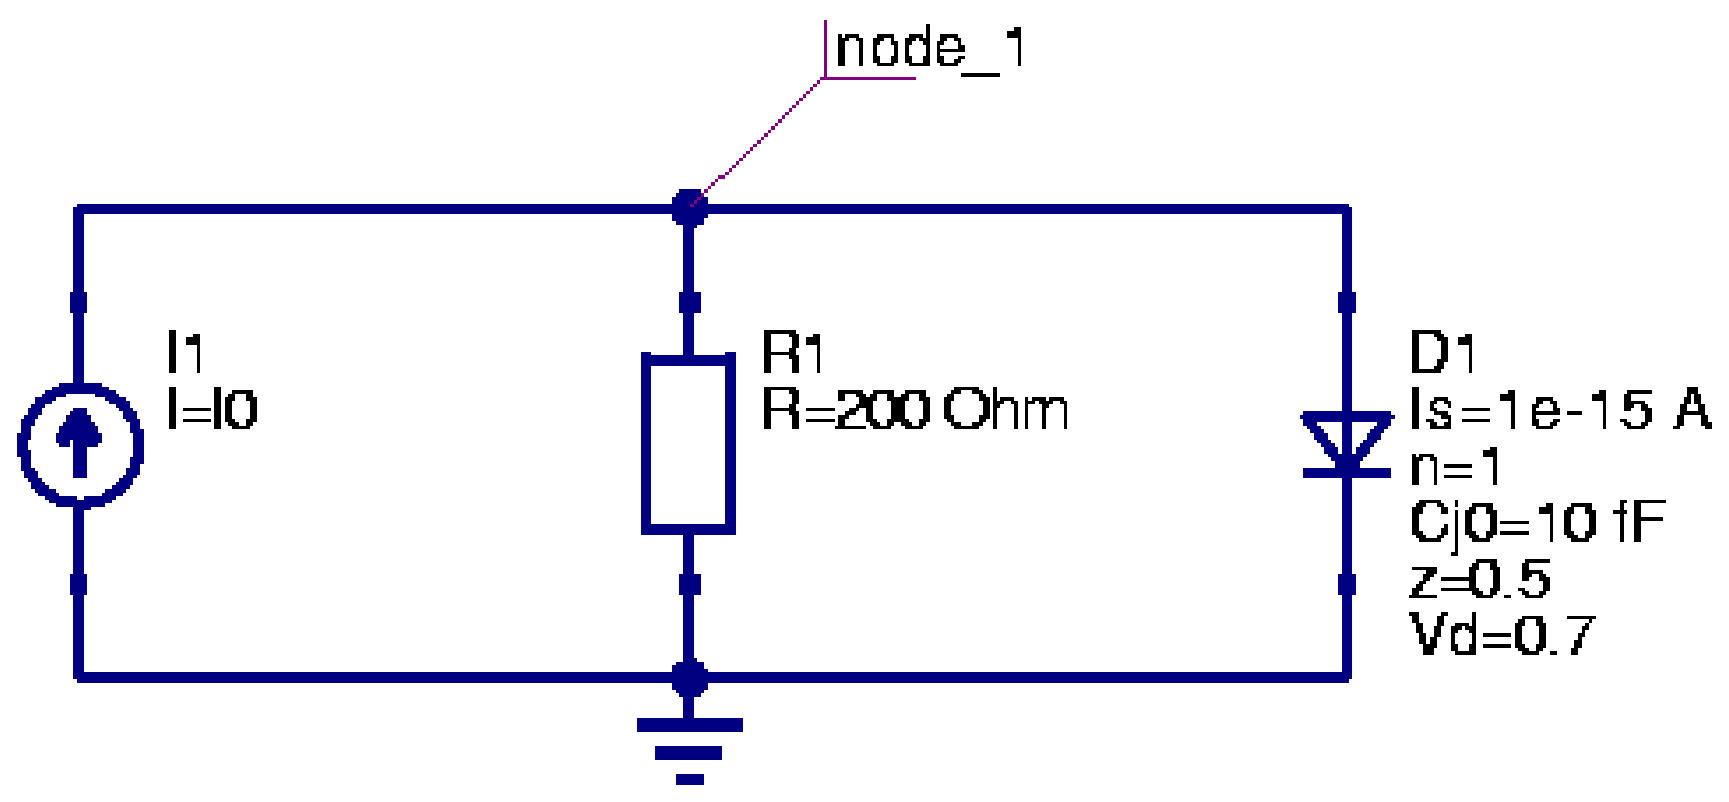
\includegraphics[width=10cm]{NLexample}
\end{center}
\caption{example circuit for non-linear DC analysis}
\label{fig:NLexample}
\end{figure}
\FloatBarrier

The 1x1 MNA equation system to be solved can be written as
\begin{equation}
\begin{bmatrix}
G
\end{bmatrix}
\cdot
\begin{bmatrix}
V_{1}
\end{bmatrix}
=
\begin{bmatrix}
I_{0}
\end{bmatrix}
\label{eq:NLmatrix}
\end{equation}

whereas the value for $G$ is now going to be explained.  The current
through a diode is simply determined by Schockley's approximation
\begin{equation}
I_{d} = I_{S}\cdot \left(e^{\frac{V_{d}}{V_{T}}} - 1\right)
\end{equation}

Thus Kirchhoff's current law at node 1 can be expressed as
\begin{equation}
I_{0} = \dfrac{V}{R} + I_{S}\cdot \left(e^{\frac{V}{V_{T}}} - 1\right)
\end{equation}

By establishing eq. (\ref{eq:NLfunc}) it is possible to trace the
problem back to finding the zero point of the function $f$.
\begin{equation}
f(V) = \dfrac{V}{R} + I_{S}\cdot \left(e^{\frac{V}{V_{T}}} - 1\right) - I_{0}
\label{eq:NLfunc}
\end{equation}

Newton developed a method stating that the zero point of a functions
derivative (i.e. the tangent) at a given point is nearer to the zero
point of the function itself than the original point.  In mathematical
terms this means to linearise the function $f$ at a starting value
$V^{(0)}$.
\begin{equation}
f\left(V^{(0)} + \Delta V\right) \approx f\left(V^{(0)}\right) + \left.\dfrac{\partial f\left(V\right)}{\partial V}\right|_{V^{(0)}}\cdot \Delta V
\;\;\;\; \text{ with } \;\;\;\;
\Delta V = V^{(1)} - V^{(0)}
\label{eq:NRapprox}
\end{equation}

Setting $f(V^{(1)}) = 0$ gives
\begin{equation}
V^{(1)} = V^{(0)} - \dfrac{f\left(V^{(0)}\right)}{\left.\dfrac{\partial f\left(V\right)}{\partial V}\right|_{V^{(0)}}}
\end{equation}

or in the general case with $m$ being the number of iteration
\begin{equation}
V^{(m + 1)} = V^{(m)} - \dfrac{f\left(V^{(m)}\right)}{\left.\dfrac{\partial f\left(V\right)}{\partial V}\right|_{V^{(m)}}}
\label{eq:NRgeneral}
\end{equation}

This must be computed until $V^{(m+1)}$ and $V^{(m)}$ differ less than a
certain barrier.
\begin{equation}
\left|V^{(m+1)} - V^{(m)}\right| < \varepsilon_{abs} + \varepsilon_{rel}\cdot \left|V^{(m)}\right|
\label{eq:NLconvergence}
\end{equation}

With very small $\varepsilon_{abs}$ the iteration would break too
early and for little $\varepsilon_{rel}$ values the iteration aims to
a useless precision for large absolute values of $V$.

\begin{figure}[ht]
\begin{center}
\psfrag{V0}{$\mathrm{V^{(0)}}$}
\psfrag{V1}{$\mathrm{V^{(1)}}$}
\psfrag{V2}{$\mathrm{V^{(2)}}$}
\includegraphics[width=0.75\linewidth]{newton}
\end{center}
\caption{Newton-Raphson method for example circuit}
\label{fig:NewtonRaphson}
\end{figure}
\FloatBarrier

With this theoretical background it is now possible to step back to
eq. (\ref{eq:NLfunc}) being the determining equation for the example
circuit.  With
\begin{equation}
g_{d}^{(m)} = \left.\dfrac{\partial I_{d}}{\partial V}\right|_{V^{(m)}} = \dfrac{I_{S}}{V_{T}}\cdot e^{\frac{V^{(m)}}{V_{T}}}
\end{equation}

and
\begin{equation}
\left.\dfrac{\partial f\left(V\right)}{\partial V}\right|_{V^{(m)}} = \dfrac{1}{R} + g_{d}^{(m)}
\end{equation}

the eq. (\ref{eq:NRgeneral}) can be written as
\begin{equation}
\left(g_{d}^{(m)} + \dfrac{1}{R}\right)\cdot V^{(m+1)} = I_{0} - \left(I_{d}^{(m)} - g_{d}^{(m)}\cdot V^{(m)}\right)
\label{eq:NRresult}
\end{equation}

when the expression
\begin{equation}
f\left(V^{(m)}\right) = \dfrac{1}{R}\cdot V^{(m)} + I_{d}^{(m)} - I_{0}
\end{equation}

based upon eq. (\ref{eq:NLfunc}) is taken into account.  Comparing the
introductory MNA equation system in eq. (\ref{eq:NLmatrix}) with
eq. (\ref{eq:NRresult}) proposes the following equivalent circuit for
the diode model.

\begin{figure}[ht]
\begin{center}
\psfrag{gd}{$\mathrm{g_{d}^{(m)}}$}
\psfrag{Ieq}{$\mathrm{I_{d}^{(m)} - g_{d}^{(m)}\cdot V^{(m)}}$}
\includegraphics[width=0.2\linewidth]{newtondiode}
\end{center}
\caption{accompanied equivalent circuit for intrinsic diode}
\label{fig:AccompaniedModel}
\end{figure}
\FloatBarrier

\label{sec:DCdiode}

With
\begin{equation}
I_{eq} = I_{d}^{(m)} - g_{d}^{(m)}\cdot V^{(m)}
\end{equation}

the MNA matrix entries can finally be written as
\begin{equation}
\begin{bmatrix}
g_{d} & -g_{d}\\
-g_{d} & g_{d}
\end{bmatrix}
\cdot
\begin{bmatrix}
V_{1}\\
V_{2}
\end{bmatrix}
=
\begin{bmatrix}
-I_{eq}\\
I_{eq}
\end{bmatrix}
\end{equation}

In analog ways all controlled current sources with non-linear
current-voltage dependency built into diodes and transistors can be
modeled.  The left hand side of the MNA matrix (the A matrix) is
called Jacobian matrix which is going to be build in each iteration
step.  For the solution vector $x$ possibly containing currents as
well when voltage sources are in place a likely convergence criteria
as defined in eq. (\ref{eq:NLconvergence}) must be defined for the
currents.

\subsection{Convergence}
%\addcontentsline{toc}{subsection}{Convergence}
\label{sec:convergenceDC}

Numerical as well as convergence problems occur during the
Newton-Raphson iterations when dealing with non-linear device curves
as they are used to model the DC behaviour of diodes and transistors.

\addvspace{12pt}

Linearising the exponential diode eq. \eqref{eq:curve} in the forward
region a numerical overflow can occur.  The diagram in
fig. \ref{fig:NewtonBad} visualises this situation.  Starting with
$V^{(0)}$ the next iteration value gets $V^{(1)}$ which results in an
indefinite large diode current.  It can be limited by iterating in
current instead of voltage when the computed voltage exceeds a certain
value.

\addvspace{12pt}

How this works is going to be explained using the diode model shown in
fig. \ref{fig:AccompaniedModel}.  When iterating in voltage (as
normally done) the new diode current is

\begin{equation}
\hat{I}_{d}^{(m+1)} = g_{d}^{(m)} \left(\hat{V}^{(m+1)} - V^{(m)}\right) + I_{d}^{(m)}
\end{equation}

The computed value $\hat{V}^{(m+1)}$ in iteration step $m+1$ is not
going to be used for the following step when $V^{(m)}$ exceeds the
critical voltage $V_{CRIT}$ which gets explained in the below
paragraphs.  Instead, the value resulting from

\begin{equation}
I_{d}^{(m+1)} = I_{S}\cdot \left(e^{\frac{V^{(m+1)}}{n V_{T}}} - 1\right)
\end{equation}

is used (i.e. iterating in current).  With

\begin{equation}
\hat{I}_{d}^{(m+1)} \; \shortstack{!\\=} \; I_{d}^{(m+1)}
\;\;\;\; \text{ and } \;\;\;\;
g_{d}^{(m)} = \dfrac{I_{S}}{n\cdot V_{T}}\cdot e^{\frac{V^{(m)}}{n\cdot V_{T}}}
\end{equation}

the new voltage can be written as

\begin{equation}
V^{(m+1)} = V^{(m)} + n V_{T}\cdot \ln{\left(\dfrac{\hat{V}^{(m+1)} - V^{(m)}}{n V_{T}} + 1\right)}
\end{equation}

Proceeding from Shockley's simplified diode equation the critical
voltage is going to be defined.  The explained algorithm can be used
for all exponential DC equations used in diodes and transistors.

\begin{align}
I\left(V\right) &= I_{S}\cdot \left(e^{\frac{V}{n V_{T}}} - 1\right)
\label{eq:curve}\\
y\left(x\right) &= f \left(x\right)
\label{eq:explicit}
\end{align}

\begin{figure}[ht]
\begin{center}
\psfrag{V0}{$\mathrm{V^{(0)}}$}
\psfrag{V1}{$\mathrm{V^{(1)}}$}
\psfrag{V2}{$\mathrm{V^{(2)}}$}
\psfrag{VCRIT}{$\mathrm{V_{CRIT} \rightarrow}$}
\includegraphics[width=0.75\linewidth]{newtonbad}
\end{center}
\caption{numerical problem with Newton-Raphson algorithm}
\label{fig:NewtonBad}
\end{figure}
\FloatBarrier

The critical voltage $V_{CRIT}$ is the voltage where the curve radius
of eq. \eqref{eq:curve} has its minimum with $I$ and $V$ having
equally units.  The curve radius $R$ for the explicit definition in
eq. \eqref{eq:explicit} can be written as

\begin{equation}
R = \left|\dfrac{\left(1+\left(\dfrac{dy}{dx}\right)^{2}\right)^{3/2}}{\dfrac{d^{2}y}{dx^{2}}}\right|
\label{eq:radius}
\end{equation}

Finding this equations minimum requires the derivative.

\begin{equation}
\dfrac{dR}{dx} = \dfrac{\dfrac{d^{2}y}{dx^{2}} \cdot \dfrac{3}{2}\left(1+\left(\dfrac{dy}{dx}\right)^{2}\right)^{1/2} \cdot 2 \cdot \dfrac{dy}{dx} \cdot \dfrac{d^{2}y}{dx^{2}} - \left(1+\left(\dfrac{dy}{dx}\right)^{2}\right)^{3/2} \cdot \dfrac{d^{3}y}{dx^{3}}}{\left(\dfrac{d^{2}y}{dx^{2}}\right)^{2}}
\label{eq:radiusderivative}
\end{equation}

The diagram in fig. \ref{fig:radius} shows the graphs of
eq. \eqref{eq:radius} and eq. \eqref{eq:radiusderivative} with $n=1$,
$I_{S}=100\nano\ampere$ and $V_{T}=25\milli\volt$.

\begin{figure}[ht]
\begin{center}
\includegraphics[width=0.7\linewidth]{radius}
\end{center}
\caption{curve radius of exponential diode curve and its derivative}
\label{fig:radius}
\end{figure}
\FloatBarrier

With the following higher derivatives of eq. \eqref{eq:curve}

\begin{align}
\dfrac{d I\left(V\right)}{dV} &= \dfrac{I_{S}}{n V_{T}}\cdot e^{\frac{V}{n V_{T}}}\\
\dfrac{d^{2} I\left(V\right)}{dV^{2}} &= \dfrac{I_{S}}{n^{2} V_{T}^{2}}\cdot e^{\frac{V}{n V_{T}}}\\
\dfrac{d^{3} I\left(V\right)}{dV^{3}} &= \dfrac{I_{S}}{n^{3} V_{T}^{3}}\cdot e^{\frac{V}{n V_{T}}}
\end{align}

the critical voltage results in

\begin{equation}
\dfrac{dR}{dx} \;\shortstack{!\\=}\; 0 = 3 - \dfrac{n^{2} V_{T}^{2}}{I_{S}^{2}}\cdot e^{-2\frac{V}{n V_{T}}} - 1
\;\;\;\; \rightarrow \;\;\;\;
V_{CRIT} = n V_{T}\cdot \ln{\left(\dfrac{n V_{T}}{I_{S} \sqrt{2}}\right)}
\end{equation}

In order to avoid numerical errors a minimum value of the
pn-junction's derivative (i.e. the currents tangent in the operating
point) $g_{min}$ is defined.  On the one hand this avoids very large
deviations of the appropriate voltage in the next iteration step in
the backward region of the pn-junction and on the other hand it avoids
indefinite large voltages if $g_d$ itself suffers from numerical
errors and approaches zero.

\addvspace{12pt}

The quadratic input I-V curve of field-effect transistors as well as
the output characteristics of these devices can be handled in similar
ways.  The limiting (and thereby improving the convergence behaviour)
algorithm must somehow ensure that the current and/or voltage
deviation from one iteration step to the next step is not too a large
value.  Because of the wide range of existing variations how these
curves are exactly modeled there is no standard strategy to achieve
this.  Anyway, the threshold voltage $V_{Th}$ should play an important
role as well as the direction which the current iteration step
follows.


%
% This document contains the chapter about AC analysis.
%

\chapter{AC Analysis}
%\addcontentsline{toc}{chapter}{AC Analysis}

The AC analysis is a small signal analysis in the frequency domain.
Basically this type of simulation uses the same algorithms as the DC
analysis (section \ref{sec:MNA} on page \pageref{sec:MNA}).  The AC
analysis is a linear modified nodal analysis.  Thus no iterative
process is necessary.  With the Y-matrix of the components, i.e. now a
complex matrix, and the appropriate extensions it is necessary to
solve the equation system \eqref{eq:acMNA} similar to the (linear) DC
analysis.
\begin{equation}
\label{eq:acMNA}
\left[A\right] \cdot \left[x\right] = \left[z\right]
\;\;\;\; \textrm{ with } \;\;\;\;
A =
\begin{bmatrix}
Y & B\\
C & D
\end{bmatrix}
\end{equation}

\section{MNA matrix entries of reactive components}
%\addcontentsline{toc}{section}{MNA matrix entries of reactive components}

If not otherwise noted the MNA matrix elements and the extensions of
the components (section \ref{sec:MNAext} on page \pageref{sec:MNAext})
for the AC analysis do not differ from those for the DC analysis.  The
Y-matrices of the non-linear devices and certain microstrip components
are documented in the appropriate sections (see chapter
\ref{sec:NLdevices} and \ref{sec:MScomponents}).

\subsection{Capacitor}
%\addcontentsline{toc}{subsection}{Capacitor}

The Y-parameter matrix of an ideal capacitor with the capacitance $C$
writes as follows.
\begin{equation}
Y =
\begin{bmatrix}
+j\omega C & -j\omega C\\
-j\omega C & +j\omega C\\
\end{bmatrix}
\end{equation}

\subsection{Inductor}
%\addcontentsline{toc}{subsection}{Inductor}

The Y-parameter matrix of an ideal inductor with the inductance $L$
writes as follows.
\begin{equation}
Y =
\begin{bmatrix}
+\dfrac{1}{j\omega L} & -\dfrac{1}{j\omega L}\\
-\dfrac{1}{j\omega L} & +\dfrac{1}{j\omega L}\\
\end{bmatrix}
\end{equation}

\subsection{Transmission line}
%\addcontentsline{toc}{subsection}{Transmission line}

A transmission line is usually described by its ABCD-matrix.  (Note
that in ABCD-matrices, i.e. the chain matrix representation, the
current $i_2$ is defined to flow out of the output port.)
\begin{equation}
\left(\underline{A}\right) =
\begin{pmatrix}
\cosh{\left(\gamma\cdot l\right)} & Z_L\cdot \sinh{\left(\gamma\cdot l\right)}\\
\sinh{\left(\gamma\cdot l\right)} / Z_L & \cosh{\left(\gamma\cdot l\right)}
\end{pmatrix}
\end{equation}

These can easily be recalculated into impedance parameters.
\begin{align}
Z_{11} = Z_{22} &= \frac{Z_L}{\tanh{\left(\gamma\cdot l\right)}}\\
Z_{12} = Z_{21} &= \frac{Z_L}{\sinh{\left(\gamma\cdot l\right)}}
\end{align}

Or in admittance parameter representation it yields
\begin{equation}
\label{eq:TransLineY}
\begin{split}
Y_{11} = Y_{22} &= \frac{1}{Z_L \cdot \tanh{\left(\gamma\cdot l\right)}}\\
Y_{12} = Y_{21} &= \frac{-1}{Z_L\cdot \sinh{\left(\gamma\cdot l\right)}}
\end{split}
\end{equation}

whence $\gamma$ denotes the propagation constant $\alpha + j\beta$ and
$l$ is the length of the transmission line.  $Z_L$ represents the
characteristic impedance of the transmission line.  The Y-parameters
as defined by eq. \eqref{eq:TransLineY} can be used for the microstrip
line.  For an ideal, i.e. lossless, transmission lines they write
accordingly.
\begin{align}
Z_{11} = Z_{22} &= \frac{Z_L}{j\cdot\tan{\left(\beta\cdot l\right)}}\\
Z_{12} = Z_{21} &= \frac{Z_L}{j\cdot\sin{\left(\beta\cdot l\right)}}\\
Y_{11} = Y_{22} &= \frac{1}{j\cdot Z_L \cdot \tan{\left(\beta\cdot l\right)}}\\
Y_{12} = Y_{21} &= \frac{j}{Z_L\cdot \sin{\left(\beta\cdot l\right)}}
\end{align}

\subsection{Phase shifter}
%\addcontentsline{toc}{subsection}{Phase shifter}

A phase shifter is no more than an ideal transmission line with a
negative length and its Z-parameters write as follows.
\begin{align}
Z_{11} = Z_{22} &= \frac{j\cdot Z_{ref}}{\tan(\phi)}\\
Z_{12} = Z_{21} &= \frac{j\cdot Z_{ref}}{\sin(\phi)}
\end{align}

The admittance parameters required for the AC analysis result in
\begin{align}
Y_{11} = Y_{22} &= \frac{1}{j\cdot Z_{ref} \cdot \tan{\left(\phi\right)}}\\
Y_{12} = Y_{21} &= \frac{j}{Z_{ref}\cdot \sin{\left(\phi\right)}}
\end{align}

where $\phi$ denotes the actual phase shift of the device.  For a zero
phase shift ($\phi = 0$) neither the Z- nor the Y-parameters are
defined.  That is why during AC analysis a phase shifter with zero
phase shift represents an ideal short circuit regardless its reference
impedance.

\addvspace{12pt}

The MNA matrix entries of an ideal short circuit during AC and DC
analysis correspond to a voltage source with zero voltage.  The
complete MNA matrix representation writes as follows
\begin{equation}
\begin{bmatrix}
. & . & +1\\
. & . & -1\\
+1 & -1 & 0\\
\end{bmatrix}
\cdot
\begin{bmatrix}
V_1\\
V_2\\
I_{br}\\
\end{bmatrix}
=
\begin{bmatrix}
I_1\\
I_2\\
0
\end{bmatrix}
\end{equation}

whence $I_{br}$ denote the branch current through the voltage source.

\subsection{Attenuator}
%\addcontentsline{toc}{subsection}{Attenuator}

The impedance parameters of an attenuator with the power attenuation
$L$ (loss) (or power gain $G=1/L$) in reference to the impedance
$Z_{ref}$ write as follows.
\begin{align}
Z_{11} = Z_{22} &= Z_{ref}\cdot\frac{L+1}{L-1}\\
Z_{12} = Z_{21} &= Z_{ref}\cdot\frac{2\cdot\sqrt{L}}{L-1}
\end{align}

The Z-parameters can be easily converted into Y-parameters which are
required for the AC analysis.  An attenuator with a power attenuation
$L=1$ (no attenuation) yields an ideal short circuit regardless its
reference impedance very similar to the phase shifter with zero phase
shift.

\subsection{Controlled sources}
%\addcontentsline{toc}{subsection}{Controlled sources}

During AC analysis the transfer factors $G$ of the controlled sources
described in sections \ref{sec:vccs}, \ref{sec:vcvs}, \ref{sec:cccs}
and \ref{sec:ccvs} on page \pageref{sec:vccs} ff. result in a complex
value depending on the delay time $T$ and frequency $f$.
\begin{equation}
\underline{G} = G\cdot e^{j\omega T} = G\cdot e^{j\cdot 2\pi f\cdot T}
\end{equation}

No more changes to the MNA matrix entries are necessary in order to
use those of the DC analysis for the AC analysis.

\section{Other AC components}
%\addcontentsline{toc}{section}{Other AC components}

The following sections describe the MNA matrix entries required for
the small signal AC analysis of the remaining components not yet
discussed in previous sections.  Only components whose MNA matrix
entries differ from the DC analysis MNA entries are taken into
account.

\subsection{DC Feed and DC Block}
%\addcontentsline{toc}{subsection}{DC Feed and DC Block}

Both of the devices exchange their role in AC and DC analysis.  Thus
the MNA matrix entries of the DC feed during DC analysis correspond to
the MNA matrix entries of the DC block during AC analysis and the
other way around.

\addvspace{12pt}

During AC analysis the DC feed corresponds to an ideal open circuit
with the MNA matrix entries
\begin{equation}
\begin{bmatrix}
. & .\\
. & .\\
\end{bmatrix}
\cdot
\begin{bmatrix}
V_1\\
V_2\\
\end{bmatrix}
=
\begin{bmatrix}
I_1\\
I_2\\
\end{bmatrix}
\end{equation}

The MNA matrix entries of a DC block correspond to an ideal short
circuit during AC analysis which is modeled by a voltage source with
zero voltage.
\begin{equation}
\begin{bmatrix}
. & . & +1\\
. & . & -1\\
+1 & -1 & 0\\
\end{bmatrix}
\cdot
\begin{bmatrix}
V_1\\
V_2\\
I_{br}\\
\end{bmatrix}
=
\begin{bmatrix}
I_1\\
I_2\\
0
\end{bmatrix}
\end{equation}

\subsection{Bias T}
%\addcontentsline{toc}{subsection}{Bias T}

Figure \ref{fig:ACbiast} denotes a combination of DC feed and DC
block.  During AC analysis node 1 and 3 simply exchange their roles in
comparison to the DC analysis.

\begin{figure}[ht]
\begin{center}
\includegraphics[width=3.5cm]{biast}
\end{center}
\caption{bias t}
\label{fig:ACbiast}
\end{figure}
\FloatBarrier

Using the port configuration shown in fig. \ref{fig:ACbiast} the
complete MNA entries of the bias t during AC analysis write as
follows.
\begin{equation}
\begin{bmatrix}
 . & . & .  & -1\\
 . & . & .  &  1\\
 . & . & .  &  0\\
-1 & 1 & 0  &  0
\end{bmatrix}
\cdot
\begin{bmatrix}
V_{1}\\
V_{2}\\
V_{3}\\
I_{out}
\end{bmatrix}
=
\begin{bmatrix}
I_{1}\\
I_{2}\\
I_{3}\\
0
\end{bmatrix}
\end{equation}

\subsection{S-parameter container with additional reference port}
%\addcontentsline{toc}{subsection}{S-parameter container with additional reference port}

The Y-parameters of a multi-port component defined by its S-parameters
as described in section \ref{sec:spfile} of page \pageref{sec:spfile}
required for a small signal AC analysis can be obtained by converting
the S-parameters into Y-parameters.


%
% This document contains the chapter about AC noise analysis.
%
% Copyright (C) 2005 Stefan Jahn <stefan@lkcc.org>
% Copyright (C) 2005 Michael Margraf <Michael.Margraf@alumni.TU-Berlin.DE>
%
% Permission is granted to copy, distribute and/or modify this document
% under the terms of the GNU Free Documentation License, Version 1.1
% or any later version published by the Free Software Foundation.
%

\chapter{AC Noise Analysis}
%\addcontentsline{toc}{chapter}{AC Noise Analysis}

\section{Definitions}

First some definition must be done:

\addvspace{12pt}

Reciprocal Networks:\\
Two networks $A$ and $B$ are reciprocal to each other if their
transimpedances have the following relation:
\begin{equation}
Z_{mn,A} = Z_{nm,B}
\end{equation}
That means: Drive the current $I$ into node $n$ of circuit $A$ and
at node $m$ the voltage $I\cdot Z_{mn,A}$ appears. In circuit $B$
it is just the way around.

\addvspace{12pt}

Adjoint Networks:\\
Network $A$ and network $B$ are adjoint to each other if the
following equation holds for their MNA matrices:
\begin{equation}
[A]^T = [B]
\end{equation}


\section{The Algorithm}

To calculate the small signal noise of a circuit, the AC noise
analysis has to be applied \cite{Blum}.  This technique uses the
principle of the AC analysis described in chapter \ref{sec:acMNA} on
page \pageref{sec:acMNA}.  In addition to the MNA matrix $A$ one needs
the noise current correlation matrix $\underline{C}_Y$ of the circuit,
that contains the equivalent noise current sources for every node on
its main diagonal and their correlation on the other positions.

\addvspace{12pt}

The basic concept of the AC noise analysis is as follows: We want the
noise voltage at node $i$, so we calculate what voltage arises due to
the noise source at node $j$.  We do that for every $n$ nodes and
after that we add all the noise voltages (by paying attention to their
correlation).  But that would mean to solve the MNA equation $n$
times.  Fortunately there is a more easy way.  One can perform the
above-mentioned $n$ steps in one single step, if the reciprocal MNA
matrix is used.  This matrix equals the MNA matrix itself, if the
network is reciprocal.  A network that only contains resistors,
capacitors, inductors, gyrators and transformers is reciprocal.

\addvspace{12pt}

The question that needs to be answered now is: How do we get the
reciprocal MNA matrix for an arbitrary network? This is equivalent to
the question: How do we get the MNA matrix of the adjoint network.
The answer is quite simple: Just transpose the MNA matrix!

\addvspace{12pt}

For any network, calculating the noise voltage at node $i$ is done by
the following three steps:
\begin{alignat}{2}
 & \text{1. Solving MNA equation:} & \qquad & \left[A\right]^T \cdot \left[x\right] =
\left[A\right]^T \cdot
\begin{bmatrix}
v \\
j \\
\end{bmatrix}
=
\begin{bmatrix}
0 \\
\vdots \\
0 \\
-1 \\
0 \\
\vdots \\
0 \\
\end{bmatrix}
\leftarrow i\text{-th row} \\
 & \text{2. Creating noise correlation matrix:} & \qquad
 & \left( \underline{C}_Y \right) \\
 & \text{3. Calculating noise voltage:} & \qquad
 & u_{noise,i} = \sqrt{\left[v\right]^T \cdot \left( \underline{C}_Y \right) \cdot \left[v\right]^*}
\end{alignat}

If the normal AC analysis has already be done with LU decomposition,
then the most time consuming work of step 1 has already be done.
\begin{equation}
\text{instead of} \qquad Y = L\cdot U \qquad \text{we have} \qquad
Y^T = U^T \cdot L^T
\end{equation}

I.e. $U^T$ becomes the new $L$ matrix and $L^T$ becomes the new $U$
matrix, and we do not need to solve the matrix equation again, because
only the right-hand side was changed.  So altogether this is a quickly
done task.  (Note that in step 3, only the subvector $[v]$ of vector
$[x]$ is used.  See section \ref{sec:xmatrix} for details on this.)

\addvspace{12pt}

If we want to know the noise voltage at another node, only the
right-hand side of step 1 changes.  That is, a new LU decomposition is
not needed.

\addvspace{12pt}

As the noise current correlation matrix contains lots of zeros, it is
not worthy to create it in the computer memory.  Instead, during its
creation, one can directly apply it to the $\left[v\right]^T$ vector.



\subsection{A Simple Example}

We have the network that is depicted in figure \ref{fig:mna_noise1}.
The MNA equation is (see chapter \ref{sec:MNA}):

\begin{equation}
[A]\cdot [x] =
\begin{bmatrix}
1/R_1 & 0\\
  G   & 1/R_2
\end{bmatrix}
\cdot
\begin{bmatrix}
U_1\\
U_2
\end{bmatrix}
=
\begin{bmatrix}
0\\
0
\end{bmatrix}
\end{equation}

\begin{figure}[ht]
\begin{center}
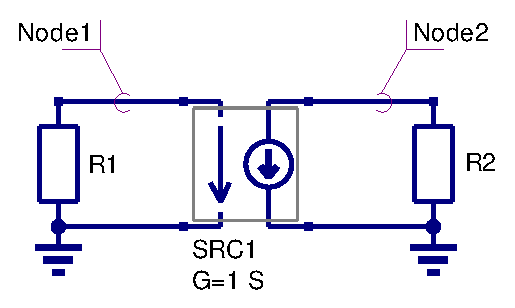
\includegraphics[width=7cm]{MNAnoise1}
\end{center}
\caption{simple non-reciprocal network}
\label{fig:mna_noise1}
\end{figure}
\FloatBarrier

Because of the controlled current source, the circuit is not
reciprocal. We want to know the noise voltage at node 2. Yes,
this is very easy to calculate, because it is a simple example,
but we want to use the algorithm described above.\\
We could solve the equations
\begin{equation}
\begin{bmatrix}
1/R_1 & 0\\
  G   & 1/R_2
\end{bmatrix}
\cdot
\begin{bmatrix}
Z_{11}\\
Z_{21}
\end{bmatrix}
=
\begin{bmatrix}
-1\\
0
\end{bmatrix}
\end{equation}
and
\begin{equation}
\begin{bmatrix}
1/R_1 & 0\\
  G   & 1/R_2
\end{bmatrix}
\cdot
\begin{bmatrix}
Z_{12}\\
Z_{22}
\end{bmatrix}
=
\begin{bmatrix}
0\\
-1
\end{bmatrix}
\end{equation}
So, we must solve the MNA matrix two times: First to get the
transimpedance from node 1 to node 2 (i.e. $Z_{21}$) and
second to get the transimpedance from node 2 to node 2 (i.e.
$Z_{22}$). But why solving it two times, if we only want to
know one voltage ? With every step we get transimpedances
that we do not need. Is there no more effective way ?

\addvspace{12pt}

Fortunately, we remember Tellegen's Theorem: A network and
its adjoint network are reciprocal to each other. That is,
we have to transpose the MNA matrix and the new matrix is
the one of the reciprocal network. Let's check it out:

\begin{equation}
[A]^T\cdot [x] =
\begin{bmatrix}
1/R_1 & G\\
  0   & 1/R_2
\end{bmatrix}
\cdot
\begin{bmatrix}
U_1\\
U_2
\end{bmatrix}
=
\begin{bmatrix}
0\\
0
\end{bmatrix}
\end{equation}

\begin{figure}[ht]
\begin{center}
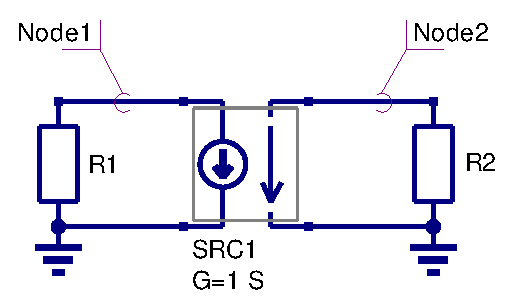
\includegraphics[width=7cm]{MNAnoise2}
\end{center}
\caption{simple network to compare with adjoint network}
\label{fig:mna_noise2}
\end{figure}
\FloatBarrier

Compare the transposed matrix with the reciprocal network
in figure \ref{fig:mna_noise2}. It is true! But now we
have:
\begin{equation}
\begin{bmatrix}
1/R_1 & G\\
  0   & 1/R_2
\end{bmatrix}
\cdot
\begin{bmatrix}
Z_{12,reciprocal}\\
Z_{22,reciprocal}
\end{bmatrix}
=
\begin{bmatrix}
1/R_1 & G\\
  0   & 1/R_2
\end{bmatrix}
\cdot
\begin{bmatrix}
Z_{21}\\
Z_{22}
\end{bmatrix}
=
\begin{bmatrix}
0\\
-1
\end{bmatrix}
\end{equation}
Because $Z_{21}$ of our original network equals $Z_{12}$ of
the reciprocal network, we get exactly what we need with one
step. So let us go on:
\begin{equation}
([A]^T)^{-1}\cdot
\begin{bmatrix}
  0\\
 -1
\end{bmatrix}
=
\begin{bmatrix}
R_1 & -G\cdot R_1\cdot R_2\\
  0 & R2
\end{bmatrix}
\cdot
\begin{bmatrix}
  0\\
 -1
\end{bmatrix}
=
\begin{bmatrix}
G\cdot R_1\cdot R_2\\
-R_2
\end{bmatrix}
=
\begin{bmatrix}
Z_{21}\\
Z_{22}
\end{bmatrix}
\end{equation}

Now, as we computed the transimpedances, we can
compute the noise voltages at node 2. As there is
no correlation, we get:

\begin{eqnarray}
<u_{node2}^2> & = & <u_{R1,node2}^2> + <u_{R2,node2}^2> \\
  & = & <i_{R1}^2>\cdot Z_{21}\cdot Z_{21}^* + <i_{R2}^2>\cdot Z_{22}\cdot Z_{22}^* \\
  & = & \frac{4\cdot k\cdot T\cdot \Delta f}{R_1} \cdot (G\cdot R_1\cdot R_2)^2 +
        \frac{4\cdot k\cdot T\cdot \Delta f}{R_2} \cdot (-R_2)^2 \\
  & = & 4\cdot k\cdot T\cdot \Delta f\cdot \left( R_1\cdot (G\cdot R_2)^2 + R_2 \right)
\end{eqnarray}

That's it. Yes, you knew it before, but now you also understand
the universal algorithm.



\section{Noise Current Correlation Matrix}
%\addcontentsline{toc}{section}{Noise Current Correlation Matrix}

This section describes the noise current correlation matrices of noisy
components.  The equations are built for RMS noise currents with
$1\hertz$ bandwidth.

\addvspace{12pt}

Resistor with resistance $R$ and temperature $T$:
\begin{equation}
(\underline{C}_Y) = \frac{4\cdot k\cdot T}{R} \cdot
\begin{pmatrix}
 1 & -1 \\
-1 &  1 \\
\end{pmatrix}
\end{equation}

Noise current source with a current power spectral density of $cPSD$:
\begin{equation}
(\underline{C}_Y) = cPSD \cdot
\begin{pmatrix}
 1 & -1 \\
-1 &  1 \\
\end{pmatrix}
\end{equation}

A noise voltage source (voltage power spectral density $vPSD$)
cannot be modeled with the noise current
matrix. That is why one has to use a noise current source
(current power spectral density $cPSD$) connected to a gyrator
(transimpedance $R$) satisfying the equation
\begin{equation}
vPSD = cPSD \cdot R
\end{equation}

Attenuator with (power) attenuation $L$, reference impedance $Z_{ref}$
and temperature $T$:
\begin{equation}
(\underline{C}_Y) = 4\cdot k\cdot T\cdot \text{Re}\left(\underline{Y}\right)
 = \frac{4\cdot k\cdot T}{Z_{ref}\cdot (L-1)} \cdot
\begin{pmatrix}
 L+1            & -2\cdot\sqrt{L} \\
-2\cdot\sqrt{L} &  L+1 \\
\end{pmatrix}
\end{equation}

Isolator with reference impedance $Z_1$ (input) and $Z_2$ (output) and
temperature $T$:
\begin{equation}
(\underline{C}_Y) = 4\cdot k\cdot T\cdot
\begin{pmatrix}
 1/Z_1                 & 0 \\
-2/\sqrt{Z_1\cdot Z_2} &  1/Z_2 \\
\end{pmatrix}
\end{equation}

Diode (for details on the parameters see section \ref{sec:nw_diode}):
\begin{equation}
(\underline{C}_Y)
 = 2\cdot e\cdot K\cdot \left(I_{d} + 2\cdot I_{S}\right)\cdot
\begin{pmatrix}
   1 & -1\\
  -1 &  1\\
\end{pmatrix}\\
\end{equation}


%
% This document contains the chapter about transient analysis.
%

\chapter{Transient Analysis}
%\addcontentsline{toc}{chapter}{Transient Analysis}

The transient simulation is the calculation of a networks response on
arbitrary excitations.  The results are network quantities (branch
currents and node voltages) as a function of time.  Substantial for
the transient analysis is the consideration of energy storing
components, i.e. inductors and capacitors.

\addvspace{12pt}

The relations between current and voltage of ideal capacitors and
inductors are given by
\begin{equation}
V_C(t) = \dfrac{1}{C}\int I_C(t) \cdot dt
\;\;\;\; \textrm{ and } \;\;\;\;
I_L(t) = \dfrac{1}{L}\int V_L(t) \cdot dt
\end{equation}

or in terms of differential equations
\begin{equation}
I_C(t) = C\cdot \dfrac{d V_C}{d t}
\;\;\;\; \textrm{ and } \;\;\;\;
V_L(t) = L\cdot \dfrac{d I_L}{d t}
\end{equation}

To calculate these quantities in a computer program numerical
integration methods are required.  With the current-voltage relations
of these components at hand it is possible to apply the modified nodal
analysis algorithm in order to calculate the networks response.  This
means the transient analysis attempts to find an approximation to the
analytical solution at discrete time points using numeric integration.

\section{Integration methods}
%\addcontentsline{toc}{section}{Integration methods}
\label{sec:IntegrationMethods}

The following differential equation is going to be solved.
\begin{equation}
\dfrac{d x}{d t} = \dot{x}(t) = f(x,t)
\label{eq:IntEquation}
\end{equation}

This differential equation is transformed into an algorithm-dependent
finite difference equation by quantizing and replacing
\begin{equation}
\dot{x}(t) = \lim_{h \rightarrow 0} \dfrac{x(t+h) - x(t)}{h}
\end{equation}

by the following equation.
\begin{equation}
\dot{x}^n = \dfrac{x^{n+1} - x^{n}}{h^{n}}
\end{equation}

There are several linear single- and multi-step numerical integration
methods available, each having advantages and disadvantages concerning
aspects of stability and accuracy.  Integration methods can also be
classified into implicit and explicit methods.  Explicit methods are
inexpensive per step but limited in stability and therefore not used
in the field of circuit simulation to obtain a correct and stable
solution.  Implicit methods are more expensive per step, have better
stability and therefore suitable for circuit simulation.

\subsection{Properties of numerical integration methods}
%\addcontentsline{toc}{subsection}{Properties of numerical integration methods}

Beforehand some definitions and explanations regarding the terms often
used in the following sections are made in order to avoid bigger
confusions later on.

\begin{itemize}
\item step size\\
The step size is defined by the arguments difference of successive
solution vectors, i.e. the time step $h^n$ during transient analysis
with $n$ being the $n$-th integration step.
\begin{equation}
h^n = t^{n+1} - t ^n
\end{equation}

\item order\\
The order $k$ of an integration method is defined as follows: With two
successive solution vectors $x^{n+1}$ and $x^{n}$ given, the successor
$x^{n+1}$ can be expressed by $x^{n}$ by a finite Taylor series.  The
order of an integrations method equals the power of the step size up
to which the approximate solution of the Taylor series differs less
than $x^{n}$ from the true solution $x^{n+1}$.

\item truncation error\\
The truncation error $\varepsilon_T$ depends on the order $k$ of the
integration method and results from the remainder term of the Taylor
series.

\item stability\\
In order to obtain an accurate network solution integration methods
are required to be stable for a given step size $h$.  Various
stability definitions exist.  This property is explained more in
detail in the following sections.  Basically it determines the
usability of an integration algorithm.

\item single- and multistep methods\\
Single step methods only use $x^n$ in order to calculate $x^{n+1}$,
multi step methods use $x^i$ with $0 \le i < n$.

\item implicit and explicit methods\\
When using explicit integration methods the evaluation of the
integration formula is sufficient for each integration step.  With
implicit methods at hand it is necessary to solve an equation system
(with non-linear networks a non-linear equation system) because for
the calculation of $x^{n+1}$, apart from $x^n$ and $\dot{x}^n$, also
$\dot{x}^{n+1}$ is used.  For the transient analysis of electrical
networks the implicit methods are better qualified than the explicit
methods.
\end{itemize}

\subsection{Elementary Methods}
%\addcontentsline{toc}{subsection}{Elementary Methods}

\subsubsection{Backward Euler}
%\addcontentsline{toc}{subsubsection}{Backward Euler}

In the implicit Euler method the right hand side of
eq. \eqref{eq:IntEquation} is substituted by $f(x^n, t^n)$ which
yields
\begin{equation}
\label{eq:BEInt}
f(x,t) = f(x^n, t^n)
\;\;\;\; \rightarrow \;\;\;\;
x^{n+1} = x^n + h^n\cdot f(x^n, t^n)
\end{equation}

The backward euler integration method is a first order single-step
method.

\subsubsection{Forward Euler}
%\addcontentsline{toc}{subsubsection}{Forward Euler}

In the explicit Euler method the right hand side of
eq. \eqref{eq:IntEquation} is substituted by $f(x^{n+1}, t^{n+1})$ which
yields
\begin{equation}
f(x,t) = f(x^{n+1}, t^{n+1})
\;\;\;\; \rightarrow \;\;\;\;
x^{n+1} = x^n + h^n\cdot f(x^{n+1}, t^{n+1})
\end{equation}

The explicit Euler method has stability problems.  The step size is
limited by stability.  In general explicit time marching integration
methods are not suitable for circuit analysis where computation with
large steps may be necessary when the solution changes slowly
(i.e. when the accuracy does not require small steps).

\subsubsection{Trapezoidal method}
%\addcontentsline{toc}{subsubsection}{Trapezoidal method}

For the bilinear (also called trapezoidal) integration method $f(x,t)$
is substituted by
\begin{equation}
f(x,t) = \dfrac{1}{2}\cdot \left(f(x^{n+1}, t^{n+1}) + f(x^{n}, t^{n})\right)
\end{equation}

which yields
\begin{equation}
\label{eq:TRInt}
x^{n+1} = x^n + \dfrac{h^n}{2}\cdot \left(f(x^{n+1}, t^{n+1}) + f(x^{n}, t^{n})\right)
\end{equation}

In each integration step the average value of the intervals beginning
and end is taken into account.  The trapezoidal rule integration
method is a second order single-step method.  There is no more
accurate second order integration method than the trapezoidal method.

\begin{center}
\begin{figure}[ht]
\begin{minipage}[t]{0.33\linewidth}
\centering
\includegraphics[height=1.8cm]{feuler}
forward-euler
\end{minipage}
\begin{minipage}[t]{0.33\linewidth}
\centering
\includegraphics[height=1.8cm]{beuler}
backward-euler
\end{minipage}
\begin{minipage}[t]{0.33\linewidth}
\centering
\includegraphics[height=1.8cm]{trapez}
trapezoidal
\end{minipage}
\end{figure}
\FloatBarrier
\end{center}

\subsection{Linear Multistep Methods}
%\addcontentsline{toc}{subsection}{Linear Multistep Methods}

For higher order multi-step integration methods the general purpose
method of resolution for the equation $\dot{x} = f(x,t)$
\begin{equation}
\label{eq:GenPurposeInt}
x^{n+1} = \sum^p_{i=0} a_i\cdot x^{n-i} + h \sum^p_{i=-1} b_i\cdot f(x^{n-i}, t^{n-i})
\end{equation}

is used.  With $b_{-1} = 0$ the method is explicit and therefore not
suitable for obtaining the correct and stable solution.  When $b_{-1}
\ne 0$ the method is implicit and suitable for circuit simulation,
i.e. suitable for solving stiff problems.  For differential equation
systems describing electrical networks the eigenvalues strongly vary.
These kind of differential equation systems are called stiff.

\addvspace{12pt}

For a polynom of order $k$ the number of required coefficients is
\begin{equation}
\label{eq:MultiStepCondition}
2p + 3 \ge k + 1
\end{equation}

The $2p +3$ coeffcients are choosen to satisfy
\begin{equation}
x^{n+1} = x(t^{n+1})
\end{equation}

This can be achieved by the following equation system
\begin{equation}
\begin{split}
\label{eq:MultiStepSys}
\sum^p_{i=0} a_i = 1\\
\sum^p_{i=1} (-i)^j a_i + j \sum^p_{i=-1} (-i)^{j-1} b_i = 1 & \textrm{ for } j = 1\ldots k
\end{split}
\end{equation}

The different linear multistep integration methods which can be
constructed by the equation system \eqref{eq:MultiStepSys} vary in the
equality condition corresponding with \eqref{eq:MultiStepCondition}
and the choice of coefficients which are set to zero.

\subsubsection{Gear}
%\addcontentsline{toc}{subsubsection}{Gear}

The Gear \cite{Gear} formulae (also called BDF - backward
differentiation formulae) have great importance within the multi-step
integration methods used in transient analysis programs.  The
conditions
\begin{equation}
p = k - 1
\;\;\;\; \textrm{ and } \;\;\;\;
b_0 = b_1 = \ldots = b_{k-1} = 0
\end{equation}

due to the following equation system
\begin{equation}
\label{eq:GearCoeff}
\left[\begin{array}{lrrrr}
0 & 1 &  1 &  1 &   1\\
1 & 0 & -1 & -2 &  -3\\
2 & 0 &  1 &  4 &   9\\
3 & 0 & -1 & -8 & -27\\
4 & 0 &  1 & 16 &  81\\
\end{array}\right]
\cdot
\begin{bmatrix}
b_{-1}\\
a_0\\
a_1\\
a_2\\
a_3\\
\end{bmatrix}
=
\begin{bmatrix}
1\\
1\\
1\\
1\\
1\\
\end{bmatrix}
\end{equation}

for the Gear formulae of order $4$.  Order $k = 1$ yields the implicit
Euler method.  The example given in the equation system
\eqref{eq:GearCoeff} results in the following integration formula.
\begin{equation}
\label{eq:GearInt}
\begin{split}
x^{n+1} &= a_0\cdot x^{n} + a_1\cdot x^{n-1} + a_2\cdot x^{n-2} + a_3\cdot x^{n-3} + h\cdot b_{-1}\cdot f(x^{n+1}, t^{n+1})\\
&= \dfrac{48}{25}\cdot x^{n} - \dfrac{36}{25}\cdot x^{n-1} + \dfrac{16}{25}\cdot x^{n-2} - \dfrac{3}{25}\cdot x^{n-3} + h\cdot \dfrac{12}{25}\cdot f(x^{n+1}, t^{n+1})
\end{split}
\end{equation}

There is no more stable second order integration method than the
Gear's method of second order.  Only implicit Gear methods with order
$k \le 6$ are zero stable.

\subsubsection{Adams-Bashford}
%\addcontentsline{toc}{subsubsection}{Adams-Bashford}

The Adams-Bashford algorithm is an explicit multi-step integration
method whence
\begin{equation}
p = k - 1
\;\;\;\; \textrm{ and } \;\;\;\;
a_1 = a_2 = \ldots = a_{k-1} = 0
\;\;\;\; \textrm{ and } \;\;\;\;
b_{-1} = 0
\end{equation}

is set to satisfy the equation system \eqref{eq:MultiStepSys}.  The
equation system of the Adams-Bashford coefficients of order 4 is as
follows.
\begin{equation}
\left[\begin{array}{lrrrr}
1 & 0 &  0 &   0 &    0\\
0 & 1 &  1 &   1 &    1\\
0 & 0 & -2 &  -4 &   -6\\
0 & 0 &  3 &  12 &   27\\
0 & 0 & -4 & -32 & -108\\
\end{array}\right]
\cdot
\begin{bmatrix}
a_0\\
b_0\\
b_1\\
b_2\\
b_3\\
\end{bmatrix}
=
\begin{bmatrix}
1\\
1\\
1\\
1\\
1\\
\end{bmatrix}
\end{equation}

This equation system results in the following integration formula.
\begin{equation}
\begin{split}
x^{n+1} &= a_0\cdot x^{n} + h\cdot b_{0}\cdot f^{n} + h\cdot b_{1}\cdot f^{n-1} + h\cdot b_{2}\cdot f^{n-2} + h\cdot b_{3}\cdot f^{n-3}\\
&= x^{n} + h\cdot \dfrac{55}{24}\cdot f^{n} - h\cdot \dfrac{59}{24}\cdot f^{n-1} + h\cdot \dfrac{37}{24}\cdot f^{n-2} - h\cdot \dfrac{9}{24}\cdot f^{n-3}\\
\end{split}
\end{equation}

The Adams-Bashford formula of order 1 yields the backward Euler
integration method.

\subsubsection{Adams-Moulton}
%\addcontentsline{toc}{subsubsection}{Adams-Moulton}

The Adams-Moulton algorithm is an implicit multi-step integration
method whence
\begin{equation}
p = k - 2
\;\;\;\; \textrm{ and } \;\;\;\;
a_1 = a_2 = \ldots = a_{k-2} = 0
\end{equation}

is set to satisfy the equation system \eqref{eq:MultiStepSys}.  The
equation system of the Adams-Moulton coefficients of order 4 is as
follows.
\begin{equation}
\left[\begin{array}{lrrrr}
1 & 0 &  0 &   0 &    0\\
0 & 1 &  1 &   1 &    1\\
0 & 2 &  0 &  -2 &   -4\\
0 & 3 &  0 &   3 &   12\\
0 & 4 &  0 &  -4 &  -32\\
\end{array}\right]
\cdot
\begin{bmatrix}
a_0\\
b_{-1}\\
b_0\\
b_1\\
b_2\\
\end{bmatrix}
=
\begin{bmatrix}
1\\
1\\
1\\
1\\
1\\
\end{bmatrix}
\end{equation}

This equation system results in the following integration formula.
\begin{equation}
\label{eq:MoultonInt}
\begin{split}
x^{n+1} &= a_0\cdot x^{n} + h\cdot b_{-1}\cdot f^{n+1} + h\cdot b_{0}\cdot f^{n} + h\cdot b_{1}\cdot f^{n-1} + h\cdot b_{2}\cdot f^{n-2}\\
&= x^{n} + h\cdot \dfrac{9}{24}\cdot f^{n+1} + h\cdot \dfrac{19}{24}\cdot f^{n} - h\cdot \dfrac{5}{24}\cdot f^{n-1} + h\cdot \dfrac{1}{24}\cdot f^{n-2}\\
\end{split}
\end{equation}

The Adams-Moulton formula of order 1 yields the forward Euler
integration method and the formula of order 2 yields the trapezoidal
rule.

\subsection{Stability considerations}
%\addcontentsline{toc}{subsection}{Stability considerations}

When evaluating the numerical formulations given for both implicit and
explicit integration formulas once rounding errors are unavoidable.
For small values of $h$ the evaluation must be repeated very often and
thus the rounding error possibly accumulates.  With higher order
algorithms it is possible to enlarge the step width and thereby reduce
the error accumulation.

\addvspace{12pt}

On the other hand it is questionable whether the construction of
implicit algorithms is really valuable because of the higher
computation effort caused by the necessary iteration (indices
$~^{n+1}$ on both sides of the equation).  In practice there is a class
of differential equations which can be reasonably handled by implicit
algorithms where explicit algorithms completely fail because of the
impracticable reduction of the step width.  This class of differential
equations are called stiff problems.  The effect of stiffness causes
for small variations in the actual solution to be computed very large
deviations in the solution which get damped.

\addvspace{12pt}

The numerical methods used for the transient analysis are required to
be stiffly stable and accurate as well.  The regions requirements in
the complex plane are visualized in the following figure.

\begin{figure}[ht]
\begin{center}
\psfrag{Re(lh)}{$\mathrm{Re \left\{h\lambda\right\}}$}
\psfrag{Im(lh)}{$\mathrm{Im \left\{h\lambda\right\}}$}
\includegraphics[width=0.7\linewidth]{stiffstable}
\end{center}
\caption{stability requirements for stiff differential equation systems}
\label{fig:StiffStable}
\end{figure}
\FloatBarrier

For values of $h\lambda$ in region II the numerical method must be
stable and accurate, in region I accurate and in region III only
stable.  The area outside the specified regions are of no particular
interest.

\addvspace{12pt}

For the stability prediction of integration algorithms with regard to
nonlinear differential equations and equation systems the simple and
linear test differential equation
\begin{equation}
\dot{x} = \lambda x
\;\;\;\; \textrm{ with } \;\;\;\;
\lambda \in \mathbb{C}, \text{Re}\left\{\lambda\right\} < 0, x \ge 0
\end{equation}

is used.  The condition $\text{Re}\left\{\lambda\right\} < 0$ ensures
the solution to be decreasing.  The general purpose method of
resolution given in \eqref{eq:GenPurposeInt} can be solved by the
polynomial method setting
\begin{equation}
x^k = z^k
\;\;\;\; \textrm{ with } \;\;\;\;
z \in \mathbb{C}
\end{equation}

Thus we get the characteristic polynom
\begin{align}
\label{eq:characteristicPolynom}
\varphi\left(z\right) &= \varrho\left(z\right) + h\lambda \cdot \eta\left(z\right) = 0\\
&= \sum^{n-1}_{i=-1} a_i\cdot z^{n-i} + h\lambda \sum^{n-1}_{i=-1} b_i\cdot z^{n-i}
\end{align}

Because of the conditions defined by \eqref{eq:MultiStepSys} the above
eq. \eqref{eq:characteristicPolynom} can only be true for
\begin{equation}
\left|z\right| < 1
\end{equation}

which describes the inner unity circle on the complex plane.  In order
to compute the boundary of the area of absolute stability it is
necessary to calculate
\begin{equation}
\label{eq:StabArea}
\mu\left(z\right) = h\lambda = -\dfrac{\varrho\left(z\right)}{\eta\left(z\right)}
\;\;\;\; \textrm{ with } \;\;\;\;
z = e^{j\vartheta}, 0 \le \vartheta \le 2\pi
\end{equation}

These equations describe closed loops. The inner of these loops
describe the area of absolute stability.  Because $\lambda \le 0$ and
$h \ge 0$ only the left half of the complex plane is of particular
interest.  An integration algorithm is call zero-stable if the
stability area encloses $\mu = 0$.  Given this condition the algorithm
is as a matter of principle usable, otherwise not.  If an algorithms
stability area encloses the whole left half plane it is called
A-stable.  A-stable algorithms are stable for any $h$ and all $\lambda
< 0$.  Any other kind of stability area introduces certain
restrictions for $\mu$.

\begin{figure}[ht]
\begin{center}
\psfrag{Re(lh)}{$\mathrm{Re \left\{h\lambda\right\}}$}
\psfrag{Im(lh)}{$\mathrm{Im \left\{h\lambda\right\}}$}
\includegraphics[width=1\linewidth]{stabgear}
\end{center}
\caption{areas of absolute stability for order 1\ldots 6 Gear formulae}
\label{fig:StabGear}
\end{figure}
\FloatBarrier

\begin{figure}[ht]
\begin{center}
\psfrag{Re(lh)}{$\mathrm{Re \left\{h\lambda\right\}}$}
\psfrag{Im(lh)}{$\mathrm{Im \left\{h\lambda\right\}}$}
\includegraphics[width=1\linewidth]{stabmoulton}
\end{center}
\caption{areas of absolute stability for order 1\ldots 6 Adams-Moulton formulae}
\label{fig:StabMoulton}
\end{figure}
\FloatBarrier

\begin{figure}[ht]
\begin{center}
\psfrag{Re(lh)}{$\mathrm{Re \left\{h\lambda\right\}}$}
\psfrag{Im(lh)}{$\mathrm{Im \left\{h\lambda\right\}}$}
\includegraphics[width=1\linewidth]{stabbashford}
\end{center}
\caption{areas of absolute stability for order 1\ldots 6 Adams-Bashford formulae}
\label{fig:StabBashford}
\end{figure}
\FloatBarrier

The figures \ref{fig:StabGear}, \ref{fig:StabMoulton} and
\ref{fig:StabBashford} visualize the evaluation of
eq. \eqref{eq:StabArea} for the discussed integration methods.  All of
the implicit formulae are zero-stable, thus principally usable.  The
forward Euler, Gear order 2 and the trapezoidal integration methods
are A-stable.  Fig. \ref{fig:StabGear} shows why the Gear formulae are
of such great importance for the transient analysis of electrical
networks.  With least restrictions for $\mu$ they can be stabilized.

\section{Predictor-corrector methods}
%\addcontentsline{toc}{section}{Predictor-corrector methods}

In section \ref{sec:IntegrationMethods} on pages
\pageref{sec:IntegrationMethods} ff. various integration methods have
been discussed.  The elementary as well as linear multistep methods
(in order to get more accurate methods) always assumed $a_{-1} = -1$
in its general form.  Explicit methods were encountered by $b_{-1} =
0$ and implicit methods by $b_{-1} \ne 0$.  Implicit methods have been
shown to have a limited area of stability and explicit methods to have
a larger range of stability.  With increasing order $k$ the linear
multistep methods interval of absolute stability (intersection of the
area of absolute stability in the complex plane with the real axis)
decreases except for the implicit Gear formulae.

\addvspace{12pt}

For these given reasons implicit methods can be used to obtain
solutions of ordinary differential equation systems describing so
called stiff problems.  Now considering e.g. the implicit
Adams-Moulton formulae of order 3
\begin{equation}
\label{eq:AM3}
x^{n+1} = x^{n} + h\cdot \dfrac{5}{12}\cdot f^{n+1} + h\cdot \dfrac{8}{12}\cdot f^{n} - h\cdot \dfrac{1}{12}\cdot f^{n-1}
\end{equation}

clarifies that $f^{n+1}$ is necessary to calculate $x^{n+1}$ (and the
other way around as well).  Every implicit integration method has this
particular property.  The above equation can be solved using
iteration.  This iteration is said to be convergent if the integration
method is consistent and zero-stable.  A linear multistep method that
is at least first-order is called a consistent method.  Zero-stability
and consistency are necessary for convergence.  The converse is also
true.

\addvspace{12pt}

The iteration introduces a second index $m$.
\begin{equation}
\label{eq:AM3iterate}
x^{n+1,m+1} = x^{n} + h\cdot \dfrac{5}{12}\cdot f^{n+1,m} + h\cdot \dfrac{8}{12}\cdot f^{n} - h\cdot \dfrac{1}{12}\cdot f^{n-1}
\end{equation}

This iteration will converge for an arbitrary initial guess
$x^{n+1,0}$ only limited by the step size $h$.  In practice successive
iterations are processed unless
\begin{equation}
\left|x^{n+1,m+1} - x^{n+1,m}\right| < \varepsilon_{abs} + \varepsilon_{rel}\cdot \left|x^{n+1,m}\right|
\end{equation}

The disadvantage for this method is that the number of iterations
until it converges is unknown.  Alternatively it is possible to use a
fixed number of correction steps.  A cheap way of providing a good
initial guess $x^{n+1,0}$ is using an explicit integration method,
e.g. the Adams-Bashford formula of order 3.
\begin{equation}
\label{eq:AB3}
x^{n+1,0} = x^{n} + h\cdot \dfrac{23}{12}\cdot f^{n} - h\cdot \dfrac{16}{12}\cdot f^{n-1} + h\cdot \dfrac{5}{12}\cdot f^{n-2}
\end{equation}

Equation \eqref{eq:AB3} requires no iteration process and can be used
to obtain the initial guess.  The combination of evaluating a single
explicit integration method (the predictor step) in order to provide a
good initial guess for the successive evaluation of an implicit method
(the corrector step) using iteration is called predictor-corrector
method.  The motivation using an implicit integration method is its
fitness for solving stiff problems.  The explicit method (though
possibly unstable) is used to provide a good initial guess for the
corrector steps.

\subsection{Order and local truncation error}
%\addcontentsline{toc}{subsection}{Order and local truncation error}

The order of an integration method results from the truncation error
$\varepsilon_T$ which is defined as
\begin{equation}
\varepsilon_T = x\left(t^{n+1}\right) - x^{n+1}
\end{equation}

meaning the deviation of the exact solution $x\left(t^{n+1}\right)$
from the approximate solution $x^{n+1}$ obtained by the integration
method.  For explicit integration methods with $b_{-1} = 0$ the local
truncation error $\varepsilon_{LTE}$ yields
\begin{equation}
\varepsilon_{LTE} = x\left(t^{n+1}\right) - x^{n+1}
\end{equation}

and for implicit integration methods with $b_{-1} \ne 0$ it is
\begin{equation}
\varepsilon_{LTE} \approx x\left(t^{n+1}\right) - x^{n+1}
\end{equation}

Going into equation \eqref{eq:GenPurposeInt} and setting $a_{-1} = -1$
the truncation error is defined as
\begin{equation}
\label{eq:LTE}
\varepsilon_{LTE} = \sum^p_{i=-1} a_i\cdot x\left(t^{n-i}\right) + h \sum^p_{i=-1} b_i\cdot f(x\left(t^{n-i}\right), t^{n-i})
\end{equation}

With the Taylor series expansions
\begin{align}
x\left(t^{n+i}\right) &= x\left(t^{n}\right) + \dfrac{\left(ih\right)}{1!} \dot{x}\left(t^{n}\right) + \dfrac{\left(ih\right)^2}{2!} \ddot{x}\left(t^{n}\right) + \ldots\\
f(x\left(t^{n+i}\right), t^{n+i}) = \dot{x}\left(t^{n+i}\right) &= \dot{x}\left(t^{n}\right) + \dfrac{\left(ih\right)}{1!} \ddot{x}\left(t^{n}\right) + \dfrac{\left(ih\right)^2}{2!} \dddot{x}\left(t^{n}\right) + \ldots
\end{align}

the local truncation error as defined by eq. \eqref{eq:LTE} can be
written as
\begin{equation}
\varepsilon_{LTE} = C_0\cdot x\left(t^n\right) + C_1 h\cdot \dot{x}\left(t^n\right) + C_2 h^2\cdot \ddot{x}\left(t^n\right) + \ldots
\end{equation}

The error terms $C_0$, $C_1$ and $C_2$ in their general form can then
be expressed by the following equation.
\begin{equation}
\label{eq:ErrorConstant}
C_{q} = -\dfrac{1}{q!}\cdot \sum_{i=-1}^{p-1} a_i\cdot \left(p - i\right)^{q} - \dfrac{1}{\left(q - 1\right)!} \sum_{i=-1}^{p-1} b_i\cdot \left(p - i\right)^{q - 1}
\end{equation}

A linear multistep integration method is of order $k$ if
\begin{equation}
\varepsilon_{LTE} = C_{k+1}\cdot h^{k+1}\cdot x^{(k+1)}\left(t^n\right) + O\left(h^{k+2}\right)
\end{equation}

The error constant $C_{k+1}$ of an $p$-step integration method of
order $k$ is then defined as
\begin{equation}
C_{k+1} = -\dfrac{1}{\left(k + 1\right)!}\cdot \sum_{i=-1}^{p-1} a_i\cdot \left(p - i\right)^{k+1} - \dfrac{1}{k!} \sum_{i=-1}^{p-1} b_i\cdot \left(p - i\right)^k
\end{equation}

The practical computation of these error constants is now going to be
explained using the Adams-Moulton formula of order 3 given by
eq. \eqref{eq:AM3}.  For this third order method with $a_{-1} = -1$,
$a_0=1$, $b_{-1}=5/12$, $b_0=8/12$ and $b_1=-1/12$ the following
values are obtained using eq. \eqref{eq:ErrorConstant}.
\begin{align}
C_0 &= -\dfrac{1}{0!}\cdot\left(-1\cdot 2^0 + 1\cdot 1^0\right) = 0\\
C_1 &= -\dfrac{1}{1!}\cdot\left(-1\cdot 2^1 + 1\cdot 1^1\right)
       -\dfrac{1}{0!}\cdot\left(\dfrac{5}{12} 2^0 + \dfrac{8}{12} 1^0 - \dfrac{1}{12} 0^0\right) = 0\\
C_2 &= -\dfrac{1}{2!}\cdot\left(-1\cdot 2^2 + 1\cdot 1^2\right)
       -\dfrac{1}{1!}\cdot\left(\dfrac{5}{12} 2^1 + \dfrac{8}{12} 1^1 - \dfrac{1}{12} 0^1\right) = 0\\
C_3 &= -\dfrac{1}{3!}\cdot\left(-1\cdot 2^3 + 1\cdot 1^3\right)
       -\dfrac{1}{2!}\cdot\left(\dfrac{5}{12} 2^2 + \dfrac{8}{12} 1^2 - \dfrac{1}{12} 0^2\right) = 0\\
C_4 &= -\dfrac{1}{4!}\cdot\left(-1\cdot 2^4 + 1\cdot 1^4\right)
       -\dfrac{1}{3!}\cdot\left(\dfrac{5}{12} 2^3 + \dfrac{8}{12} 1^3 - \dfrac{1}{12} 0^3\right) = -\dfrac{1}{24}
\end{align}

In similar ways it can be verified for each of the discussed linear
multistep integration methods that
\begin{equation}
C_p = 0 \;\;\;\; \forall \;\;\;\; 0 \le p \le k
\end{equation}

The following table summarizes the error constants for the implicit
Gear formulae (also called BDF - backward differention formulae).

\begin{center}
\begin{tabular}{r|c|c|c|c|c|c}
\setlength{\fboxsep}{6pt}
& \multicolumn{6}{c}{implicit Gear formulae (BDF)}\\
\hline
\setlength{\fboxrule}{0pt}
\fbox{steps $n$} & 1 & 2 & 3 & 4 & 5 & 6\\
\hline
\setlength{\fboxrule}{0pt}
\fbox{order $k$} & 1 & 2 & 3 & 4 & 5 & 6\\
\hline
error constant $C_{k+1}$ & $-\dfrac{1}{2}$ & $-\dfrac{2}{9}$ & $-\dfrac{3}{22}$ & $-\dfrac{12}{125}$ & $-\dfrac{10}{137}$ &
\setlength{\fboxrule}{0pt}
\fbox{$-\dfrac{20}{343}$}
\end{tabular}
\end{center}

The following table summarizes the error constants for the explicit
Gear formulae.

\begin{center}
\begin{tabular}{r|c|c|c|c|c|c}
\setlength{\fboxsep}{6pt}
& \multicolumn{6}{c}{explicit Gear formulae}\\
\hline
\setlength{\fboxrule}{0pt}
\fbox{steps $n$} & 2 & 3 & 4 & 5 & 6 & 7\\
\hline
\setlength{\fboxrule}{0pt}
\fbox{order $k$} & 1 & 2 & 3 & 4 & 5 & 6\\
\hline
error constant $C_{k+1}$ & $+1$ & $+1$ & $+1$ & $+1$ & $+1$ &
\setlength{\fboxrule}{0pt}
\fbox{$+1$}
\end{tabular}
\end{center}

The following table summarizes the error constants for the explicit
Adams-Bashford formulae.

\begin{center}
\begin{tabular}{r|c|c|c|c|c|c}
\setlength{\fboxsep}{6pt}
& \multicolumn{6}{c}{explicit Adams-Bashford}\\
\hline
\setlength{\fboxrule}{0pt}
\fbox{steps $n$} & 1 & 2 & 3 & 4 & 5 & 6\\
\hline
\setlength{\fboxrule}{0pt}
\fbox{order $k$} & 1 & 2 & 3 & 4 & 5 & 6\\
\hline
error constant $C_{k+1}$ & $\dfrac{1}{2}$ & $\dfrac{5}{12}$ & $\dfrac{3}{8}$ &
\setlength{\fboxrule}{0pt}
\fbox{$\dfrac{251}{720}$} & $\dfrac{95}{288}$ & $\dfrac{19087}{60480}$
\end{tabular}
\end{center}

The following table summarizes the error constants for the implicit
Adams-Moulton formulae.

\begin{center}
\begin{tabular}{r|c|c|c|c|c|c}
\setlength{\fboxsep}{6pt}
& \multicolumn{6}{c}{implicit Adams-Moulton}\\
\hline
\setlength{\fboxrule}{0pt}
\fbox{steps $n$} & 1 & 1 & 2 & 3 & 4 & 5\\
\hline
\setlength{\fboxrule}{0pt}
\fbox{order $k$} & 1 & 2 & 3 & 4 & 5 & 6\\
\hline
error constant $C_{k+1}$ & $-\dfrac{1}{2}$ & $-\dfrac{1}{12}$ & $-\dfrac{1}{24}$ & $-\dfrac{19}{720}$ &
\setlength{\fboxrule}{0pt}
\fbox{$-\dfrac{3}{160}$} & $-\dfrac{863}{60480}$
\end{tabular}
\end{center}

\subsection{Milne's estimate}
%\addcontentsline{toc}{subsection}{Milne's estimate}

The locale truncation error of the predictor of order $k^{*}$ may be
defined as
\begin{equation}
\varepsilon^{*}_{LTE} = C^{*}_{k^{*}+1}\cdot h^{k^{*}+1}\cdot x^{(k^{*}+1)}\left(t^n\right) + O\left(h^{k^{*}+2}\right)
\end{equation}

and that of the corresponding corrector method of order $k$
\begin{equation}
\varepsilon_{LTE} = C_{k+1}\cdot h^{k+1}\cdot x^{(k+1)}\left(t^n\right) + O\left(h^{k+2}\right)
\end{equation}

If a predictor and a corrector method with same orders $k = k^{*}$ are
used the locale truncation error of the predictor-corrector method
yields
\begin{equation}
\varepsilon_{LTE} \approx \dfrac{C_{k+1}}{C^{*}_{k+1} - C_{k+1}}\cdot \left(x^{n+1, m} - x^{n+1, 0}\right)
\end{equation}

This approximation is called Milne's estimate.

\subsection{Adaptive step-size control}
%\addcontentsline{toc}{subsection}{Adaptive step-size control}

For all numerical integration methods used for the transient analysis
of electrical networks the choice of a proper step-size is essential.
If the step-size is too large, the results become inaccurate or even
completely wrong when the region of absolute stability is left.  And
if the step-size is too small the calculation requires more time than
necessary without raising the accuracy.  Usually a chosen initial
step-size cannot be used overall the requested time of calculation.

\addvspace{12pt}

Basically a step-size $h$ is chosen such that
\begin{equation}
\varepsilon_{LTE} < \varepsilon_{abs} + \varepsilon_{rel}\cdot \left|x^{n+1,m}\right|
\end{equation}

Forming a step-error quotient
\begin{equation}
q = \dfrac{\varepsilon_{LTE}}{\varepsilon_{abs} + \varepsilon_{rel}\cdot \left|x^{n+1,m}\right|}
\end{equation}

yields the following algorithm for the step-size control.  The initial
step size $h^0$ is chosen sufficiently small.  After each integration
step every step-error quotient gets computed and the largest $q_{max}$
is then checked.

\addvspace{12pt}

If $q_{max} > 1$, then a reduction of the current step-size is
necessary.  As new step-size the following expression is used
\begin{equation}
h^n = \left(\dfrac{\varepsilon}{q_{max}}\right)^{\tfrac{1}{k + 1}}\cdot h^n
\end{equation}

with $k$ denoting the order of the corrector-predictor method and
$\varepsilon < 1$ (e.g. $\approx 0.8)$.  If necessary the process must
be repeated.

\addvspace{12pt}

If $q_{max} > 1$, then the calculated value in the current step gets
accepted and the new step-size is
\begin{equation}
h^{n+1} = \left(\dfrac{\varepsilon}{q_{max}}\right)^{\tfrac{1}{k + 1}}\cdot h^n
\end{equation}

\section{Energy-storage components}
%\addcontentsline{toc}{section}{Energy-storage components}

As already mentioned it is essential for the transient analysis to
consider the energy storing effects of components.  The following
section describes how the modified nodal analysis can be used to take
this into account.

\subsection{Capacitor}
%\addcontentsline{toc}{subsection}{Capacitor}

The relation between current and voltage in terms of a differential
equation for an ideal capacitor is
\begin{equation}
\label{eq:ConstCap}
I_C(t) = C\cdot \dfrac{d V_C}{d t}
\end{equation}

With
\begin{equation}
\dfrac{I_C(V, t)}{C} = \dfrac{d V_C}{d t} = f(x,t)
\end{equation}

the discussed integration formulas \eqref{eq:BEInt}, \eqref{eq:TRInt},
\eqref{eq:GearInt} and \eqref{eq:MoultonInt} can be applied to the
problem.  Rewriting them in an explicit form regarding the next
integration current results in
\begin{align}
\label{eq:EulerIC}
I_C^{n+1} &= \dfrac{C}{h^{n}} V_C^{n+1} - \dfrac{C}{h^{n}} V_C^{n}\\
I_C^{n+1} &= \dfrac{2C}{h^{n}} V_C^{n+1} - \dfrac{2C}{h^{n}} V_C^{n} - I_C^n\\
I_C^{n+1} &= \dfrac{C}{b_{-1}\cdot h^{n}} V_C^{n+1} - \dfrac{a_0\cdot C}{b_{-1}\cdot h^{n}} V_C^{n} - \dfrac{a_1\cdot C}{b_{-1}\cdot h^{n}} V_C^{n-1} - \ldots - \dfrac{a_{k-1}\cdot C}{b_{-1}\cdot h^{n}} V_C^{n-k+1}\\
I_C^{n+1} &= \underbrace{\dfrac{C}{b_{-1}\cdot h^{n}}}_{g_{eq}} V_C^{n+1} \underbrace{- \dfrac{a_0\cdot C}{b_{-1}\cdot h^{n}} V_C^{n} - \dfrac{b_0}{b_{-1}} I_C^n - \dfrac{b_1}{b_{-1}} I_C^{n-1} - \ldots - \dfrac{b_{k-2}}{b_{-1}} I_C^{n-k+2}}_{I_{eq}}
\end{align}

Each of these equations can be rewritten as
\begin{equation}
I_C^{n+1} = g_{eq}\cdot V_C^{n+1} + I_{eq}
\end{equation}

which leads to the following companion model representing a current
source with its accompanied internal resistance.
\begin{figure}[ht]
\begin{center}
\includegraphics[width=0.35\linewidth]{transcap}
\end{center}
\caption{companion equivalent circuit of a capacitor during transient analysis}
\label{fig:TransCap}
\end{figure}
\FloatBarrier

Thus the complete MNA matrix equation for an ideal capacitance writes
as follows.
\begin{equation}
\begin{bmatrix}
+g_{eq} & -g_{eq}\\
-g_{eq} & +g_{eq}\\
\end{bmatrix}
\cdot
\begin{bmatrix}
V_1^{n+1}\\
V_2^{n+1}\\
\end{bmatrix}
=
\begin{bmatrix}
-I_{eq}\\
+I_{eq}\\
\end{bmatrix}
\end{equation}

\subsection{Inductor}
%\addcontentsline{toc}{subsection}{Inductor}

The relation between current and voltage in terms of a differential
equation for an ideal inductor can be written as
\begin{equation}
V_L(t) = L\cdot \dfrac{d I_L}{d t}
\end{equation}

With
\begin{equation}
\dfrac{V_L(I, t)}{L} = \dfrac{d I_L}{d t} = f(x,t)
\end{equation}

the discussed integration formulas \eqref{eq:BEInt}, \eqref{eq:TRInt},
\eqref{eq:GearInt} and \eqref{eq:MoultonInt} can be applied to the
problem.  Rewriting them in an explicit form regarding the next
integration voltage results in
\begin{align}
V_L^{n+1} &= \dfrac{L}{h^{n}} I_L^{n+1} - \dfrac{L}{h^{n}} I_L^{n}\\
V_L^{n+1} &= \dfrac{2L}{h^{n}} I_L^{n+1} - \dfrac{2L}{h^{n}} I_L^{n} - V_L^n\\
V_L^{n+1} &= \dfrac{L}{b_{-1}\cdot h^{n}} I_L^{n+1} - \dfrac{a_0\cdot L}{b_{-1}\cdot h^{n}} I_L^{n} - \dfrac{a_1\cdot L}{b_{-1}\cdot h^{n}} I_L^{n-1} - \ldots - \dfrac{a_{k-1}\cdot L}{b_{-1}\cdot h^{n}} I_L^{n-k+1}\\
V_L^{n+1} &= \underbrace{\dfrac{L}{b_{-1}\cdot h^{n}}}_{r_{eq}} I_L^{n+1} \underbrace{- \dfrac{a_0\cdot L}{b_{-1}\cdot h^{n}} I_L^{n} - \dfrac{b_0}{b_{-1}} V_L^n - \dfrac{b_1}{b_{-1}} V_L^{n-1} - \ldots - \dfrac{b_{k-2}}{b_{-1}} V_L^{n-k+2}}_{V_{eq}}
\end{align}

Each of these equations can be rewritten as
\begin{equation}
V_L^{n+1} = r_{eq}\cdot I_L^{n+1} + V_{eq}
\end{equation}

which leads to the following companion model representing a voltage
source with its accompanied internal resistance.
\begin{figure}[ht]
\begin{center}
\includegraphics[width=0.375\linewidth]{transind}
\end{center}
\caption{companion equivalent circuit of a inductor during transient analysis}
\end{figure}
\FloatBarrier

Thus the complete MNA matrix equation for an ideal inductor writes
as follows.
\begin{equation}
\begin{bmatrix}
0 & 0 & +1\\
0 & 0 & -1\\
+1 & -1 & -r_{eq}\\
\end{bmatrix}
\cdot
\begin{bmatrix}
V_1^{n+1}\\
V_2^{n+1}\\
I_L^{n+1}\\
\end{bmatrix}
=
\begin{bmatrix}
0\\
0\\
V_{eq}\\
\end{bmatrix}
\end{equation}

It also possible to model the ideal inductor as a current source with
an internal resistance which would yield a similar equivalent circuit
as for the capacitor.  But with the proposed model it is possible to
use alike computation schemes for capacitors and inductors.  Charges
become flues, capacitances become inductances and finally voltages
become currents and the other way around.  Everything else (especially
the coeffcients in the integration formulas) can be reused.

\subsection{Depletion Capacitance}
%\addcontentsline{toc}{subsection}{Depletion Capacitance}

For non-constant capacitances, especially depletion capacitance used
in non-linear devices, instead of eq. \eqref{eq:ConstCap} the
following equation holds.
\begin{equation}
I_C(t) = \dfrac{d Q}{d t}
\end{equation}

With
\begin{equation}
d Q = C\cdot d V_C
\;\;\;\; \textrm{ and } \;\;\;\;
\left.\dfrac{d V_C}{d Q}\right|_{Q^{(m)}} = \dfrac{1}{C}
\end{equation}

equation \eqref{eq:NRgeneral} can be written as
\begin{equation}
V_C^{(m + 1)} = V_C^{(m)} - \dfrac{Q\left(V_C^{(m)}\right)}{C^{(m)}}
\end{equation}

yielding a similar iterative algorithm as already used for the
non-linear DC analysis described in section \ref{sec:NRmethod} on page
\pageref{sec:NRmethod}.  The indices $~^{(m)}$ indicated the $m$-th
Newton-Raphson iteration.  With this knowledge at hand it is possible
to rewrite the explicit formula for the forward Euler integration
\eqref{eq:EulerIC} as
\begin{equation}
\begin{split}
I_C^{n+1,m} &= \dfrac{Q^{n+1,m}}{h^{n}} - \dfrac{Q^{n}}{h^{n}}\\
&= \dfrac{C^{n+1,m}}{h^{n}} V_C^{n+1} - \dfrac{C^{n}}{h^{n}} V_C^{n}
\end{split}
\end{equation}

The double indices now indicate the $n$-th integration step and the
$m$-th Newton-Raphson iteration.  The same can be done for the other
integration formulas and results also in a similar equivalent
companion model as shown in fig. \ref{fig:TransCap}.  The capacitance
$C$ within the above equations is computed according to the
appropriate (non-linear) model formulations, e.g.
\begin{equation}
C^{n+1,m} = C_{0}\cdot \left(1 - \dfrac{V_{C}^{n+1,m}}{V_{j}}\right)^{-M}
\end{equation}

\subsection{Diffusion Capacitance}
%\addcontentsline{toc}{subsection}{Diffusion Capacitance}

The current through a diffusion capacitance can be approximated by
\begin{equation}
I_C(t) = \tau_D \dfrac{d I_D}{d t}
\end{equation}

whence $\tau_D$ specifies the transit time through a pn-junction.  The
above formula can be rewritten as
\begin{equation}
I_C(t) = \tau_D \dfrac{d I_D}{d V_C}\cdot \dfrac{d V_C}{d t} = \tau_D \cdot g_D \cdot \dfrac{d V_C}{d t}
\end{equation}

which means that eq. \eqref{eq:EulerIC} yields now
\begin{equation}
\begin{split}
I_C^{n+1,m} &= \dfrac{Q^{n+1,m}}{h^{n}} - \dfrac{Q^{n}}{h^{n}}\\
&= \dfrac{\tau_D\cdot g_D^{n+1,m}}{h^{n}} V_C^{n+1} - \dfrac{\tau_D\cdot g_D^{n}}{h^{n}} V_C^{n}\\
&= \dfrac{C^{n+1,m}}{h^{n}} V_C^{n+1} - \dfrac{C^{n}}{h^{n}} V_C^{n}
\end{split}
\end{equation}

Similar to the diffusion capacitance a Newton-Raphson iteration is
necessary.  Also the formulas for the other integration methods can be
easily rewritten and the equivalent companion model shown in
fig. \ref{fig:TransCap} is valid as well.


%
% This document contains the chapter about harmonic balance analysis.
%
% Copyright (C) 2005 Stefan Jahn <stefan@lkcc.org>
% Copyright (C) 2005 Michael Margraf <Michael.Margraf@alumni.TU-Berlin.DE>
%
% Permission is granted to copy, distribute and/or modify this document
% under the terms of the GNU Free Documentation License, Version 1.1
% or any later version published by the Free Software Foundation.
%

\chapter{Harmonic Balance Analysis}
\label{sec:hb_analysis}

Harmonic balance is a non-linear, frequency-domain, steady-state
simulation.  The voltage and current sources create discrete
frequencies resulting in a spectrum of discrete frequencies at every
node in the circuit. Linear circuit components are solely modeled in
frequency domain. Non-linear components are modeled in time domain and
Fourier-transformed before each solving step.  The informations in
this chapter are taken from \cite{Maas1} (chapter 3) which is a very
nice and well-written publication on this topic.

\addvspace{12pt}

The harmonic balance simulation is ideal for situations where
transient simulation methods are problematic. These are:
\begin{itemize}
\item components modeled in frequency domain, for instance (dispersive)
      transmission lines
\item circuit time constants large compared to period of simulation
      frequency
\item circuits with lots of reactive components
\end{itemize}
Harmonic balance methods, therefore, are the best choice for most microwave
circuits excited with sinusoidal signals (e.g. mixers, power amplifiers).


\section{The Basic Concept}

As non-linear elements can only be modeled in time domain, the circuit
first must be separated into a linear and a non-linear part. The
internal impedances $Z_i$ of the voltage sources are put into the
linear part as well. Figure \ref{fig:hb_concept} illustrates the
concept. Let us define the following symbols:
\begin{description}
\item[] M = number of (independent) voltage sources
\item[] N = number of connections between linear and non-linear subcircuit
\item[] K = number of calculated harmonics
\end{description}

\begin{figure}[ht]
\begin{center}
\includegraphics[width=9cm]{hb_concept}
\end{center}
\caption{circuit partitioning in harmonic balance}
\label{fig:hb_concept}
\end{figure}
\FloatBarrier

The linear circuit is modeled by two transadmittance matrices:
The first one $(\tilde{\underline{Y}})$
relates the source voltages $v_{S,1}...v_{S,M}$ to the interconnection
currents $i_1...i_N$ and the second one $(\hat{\underline{Y}})$
relates the interconnection
voltages $v_1...v_N$ to the interconnection currents $i_1...i_N$.
Taking both, we can express the current flowing through the
interconnections between linear and non-linear subcircuit:

\begin{equation}
\label{eqn:HBlin}
(\underline{I})
  = (\underline{\tilde{Y}})\cdot (\underline{V}_S) + (\underline{\hat{Y}})\cdot (\underline{V})
  = (\underline{I}_S) + (\underline{\hat{Y}})\cdot (\underline{V})
\end{equation}
Because $(\underline{V}_S)$ is known and constant, the first term
can already be computed to give $(\underline{I}_S)$.

\addvspace{12pt}

The non-linear circuit is modeled by its current function
$i(t) = f_g(v_1, ..., v_N)$
and by the charge of its capacitances
$q(t) = f_q(v_1, ..., v_N)$.
These functions must be Fourier-transformed to give the
frequency-domain vectors $(\underline{Q})$ and $(\underline{I}_G)$,
respectively.

\addvspace{12pt}

A simulation result is found if the currents through the
interconnections are the same for the linear and the non-linear
subcircuit. So, the non-linear equation system that needs to be
solved writes:
\begin{equation}
(\underline{0})
  = (\underline{I}_S) + (\underline{\hat{Y}})\cdot (\underline{V})
    + j\cdot (\underline{\Omega})\cdot (\underline{Q}) + (\underline{I}_G)
\end{equation}
where matrix $(\underline{\Omega})$ contains the angular frequencies
on the first main diagonal and zeros anywhere else, $(\underline{0})$
is zero matrix.

\addvspace{12pt}

After each iteration step, the inverse Fourier transformation must
be applied to the voltage vector $(\underline{V})$. Then the time domain
voltages $v_1...v_N$ are put into $i(t) = f_g(v_1, ..., v_N)$
and $q(t) = f_q(v_1, ..., v_N)$ again. Now, a Fourier transformation
gives the vectors $(\underline{Q})$ and $(\underline{I}_G)$ for the
next iteration step. After repeating this several times, a simulation
result has hopefully be found.

\section{Going through each Step}

\subsection{Creating Transadmittance Matrix}

It needs several steps to get the transadmittance matrices $[\tilde{Y}]$
and $[\hat{Y}]$ mentioned in equation \eqref{eqn:HBlin}. First the MNA
matrix of the linear subcircuit (figure \ref{fig:hb_concept}) is created
(chapter \ref{sec:MNA}). Then the transimpedance matrix is derived by
exciting one by one the port nodes of the MNA matrix with unity current.
After that the transadmittance matrix is calculated by inverting the
transimpedance matrix. Finally the matrices $[\tilde{Y}]$ and $[\hat{Y}]$
are filled with the corresponding elements of the overall transadmittance
matrix.

\addvspace{12pt}

Now this should be decribed in more detail: By use of the MNA matrix
$[A]$, the $n$-th column of the transimpedance matrix $[Z]$ should be
calculated. The voltage source at port $n$ is connected to node $i$
(positive terminal) and to port $j$ (negative terminal). This results
in the following equation:
\begin{equation}
\label{eqn:HBtrans}
[A]\cdot
\begin{bmatrix}
V_1\\
\vdots\\
V_K\\
\end{bmatrix}
=
\begin{bmatrix}
0\\
\vdots\\
1\\
\vdots\\
-1\\
\vdots\\
0\\
\end{bmatrix}
\begin{matrix}
 \\
 \\
\leftarrow i\text{-th row}\\
 \\
\leftarrow j\text{-th row}\\
 \\
 \\
\end{matrix}
\end{equation}
<<<<<<< hbanalysis.tex
After having solved it, $Z_{1,n}$...$Z_{N+M,n}$ are obtained
simply by substration of the node voltages:
=======
After having solved it, we got $Z_{1,n}$...$Z_{N+M,n}$
simply by subtraction of the node voltages:
>>>>>>> 1.3
\begin{equation}
Z_{m,n} = V_k - V_l
\end{equation}
Here the voltage source at port $m$ is connected to node $k$
(positive terminal) and to node $l$ (negative terminal).

\addvspace{12pt}

The next column of $[Z]$ is obtained by changing the right-hand
side of equation \eqref{eqn:HBtrans} appropriately. As this has to
be done $N+M$ times, it is strongly recommended to use LU
decomposition.

\addvspace{12pt}

One further thing must be mentioned: Because the non-linear
components are missing in the linear MNA matrix, there are often
components that are completely disconnected from the rest of the
circuit. The resulting MNA matrix cannot be solved. To avoid
this problem, shunt each port with a $100\Omega$ resistor. The
effect of these resistors can be easily removed by subtracting
0.01S from the first main diagonal of the transadmittance matrix.


\subsection{Termination Criteria}

Frequency components with very different magnitude appear in harmonic
balance simulation. In order to detect when the solver has found an
accurate solution, an absolute as well as relative criteria must be
used on all nodes and at all frequencies. The analysis is regarded as
finished if one of the criteria is satisfied.

\addvspace{12pt}

The absolute and relative criteria write as follows:
\begin{equation}
\left| \tilde{I}_{n,k} + \hat{I}_{n,k} \right| < \epsilon_{abs}
  \qquad \text{for all} \quad n, k
\end{equation}
\begin{equation}
2\cdot \left| \frac{\tilde{I}_{n,k} + \hat{I}_{n,k}}
                   {\tilde{I}_{n,k} - \hat{I}_{n,k}} \right|
  < \epsilon_{rel}  \qquad \text{for all} \quad n, k
\end{equation}
where $\tilde{I}_{n,k}$ is the current of the linear circuit
partition for node $n$ and frequency $k$ and $\hat{I}_{n,k}$
is the current of the non-linear circuit partition.

\subsection{Frequency-Time Domain Transformation}

During every iteration step, the time domain values have to be transformed
into frequency domain and back. A standard Fourier Transformation is not
useful, because with multi-tone excitation many mixing products appear.
The best way to cope with this problem is to use two-dimensional
Fast-Fourier-Transformation (2D-FFT).


%
% This document contains the chapter about non-linear devices.
%

\chapter{Non-linear devices}
%\addcontentsline{toc}{chapter}{Non-linear devices}
\label{sec:NLdevices}

\section{PN-Junction Diode}
%\addcontentsline{toc}{section}{PN-Junction Diode}

The following table contains the model parameters for the pn-junction
diode model.

\addvspace{12pt}

\begin{tabular}{rllll}
Name & Symbol & Description & Unit & Default\\
\hline
Is & $I_{S}$ & saturation current & $\ampere$ & $10^{-14}$\\
N & $N$ & emission coefficient & & $1.0$\\
Isr & $I_{SR}$ & recombination current parameter & $\ampere$ & $0.0$\\
Nr & $N_{R}$ & emission coefficient for Isr & & $2.0$\\
Rs & $R_{S}$ & ohmic resistance & $\ohm$ & $0.0$\\
Cj0 & $C_{j0}$ & zero-bias junction capacitance & $\farad$ & $0.0$\\
M & $M$ & grading coefficient & & $0.5$\\
Vj & $V_{j}$ & junction potential & $\volt$ & $0.7$\\
Fc & $F_{c}$ & forward-bias depletion capacitance coefficient & & $0.5$\\
Cp & $C_{p}$ & linear capacitance & $\farad$ & $0.0$\\
Tt & $\tau$ & transit time & $\second$ & $0.0$\\
Kf & $K_F$ & flicker noise coefficient & & $0.0$\\
Af & $A_F$ & flicker noise exponent & & $1.0$\\
Ffe & $F_{FE}$ & flicker noise frequency exponent & & $1.0$\\
Temp & $T$ & device temperature & $\degree \mathrm{C}$ & $26.85$
\end{tabular}

\addvspace{12pt}

\subsection{Large signal model}
%\addcontentsline{toc}{subsection}{Large signal model}

\begin{figure}[ht]
\begin{center}
\includegraphics[width=0.3\linewidth]{diode}
\end{center}
\caption{pn-junction diode symbol and large signal model}
\label{fig:diode}
\end{figure}
\FloatBarrier

The current equation of the diode and its derivative writes as
follows:
\begin{align}
I_{d} &= I_{S}\cdot \left(e^{\frac{V_{d}}{N\cdot V_{T}}} - 1\right) + I_{SR}\cdot \left(e^{\frac{V_{d}}{N_R\cdot V_{T}}} - 1\right)\\
g_{d} &= \dfrac{\partial I_{d}}{\partial V_{d}} = \dfrac{I_{S}}{N\cdot V_{T}}\cdot e^{\frac{V_{d}}{N\cdot V_{T}}} + \dfrac{I_{SR}}{N_R\cdot V_{T}}\cdot e^{\frac{V_{d}}{N_R\cdot V_{T}}}
\end{align}

\begin{figure}[ht]
\begin{center}
\includegraphics[width=0.17\linewidth]{dcdiode}
\end{center}
\caption{accompanied DC model of intrinsic diode}
\label{fig:dcdiode}
\end{figure}
\FloatBarrier

The complete MNA matrix entries are:
\begin{equation}
\begin{bmatrix}
g_{d} & -g_{d}\\
-g_{d} & g_{d}\\
\end{bmatrix}
\cdot
\begin{bmatrix}
V_{C}\\
V_{A}\\
\end{bmatrix}
=
\begin{bmatrix}
+I_{d} - g_{d}\cdot V_{d}\\
-I_{d} + g_{d}\cdot V_{d}\\
\end{bmatrix}
\end{equation}

\subsection{Small signal model}
%\addcontentsline{toc}{subsection}{Small signal model}

\begin{figure}[ht]
\begin{center}
\includegraphics[width=0.17\linewidth]{spdiode}
\end{center}
\caption{small signal model of intrinsic diode}
\label{fig:spdiode}
\end{figure}
\FloatBarrier

The voltage dependent capacitance consists of a diffusion capacitance,
a junction capacitance and an additional linear capacitance which is
usually modeled by the following equations.

\begin{equation}
C_{d} = C_p + \tau \cdot g_{d} +
\begin{cases}
\begin{array}{ll}
C_{j0}\cdot \left(1 - \dfrac{V_{d}}{V_{j}}\right)^{-M} & \textrm{ for } V_{d} \le F_c\cdot V_j\\
\dfrac{C_{j0}}{\left(1 - F_c\right)^M}\cdot \left(1 + \dfrac{M\cdot \left(V_{d} - F_c\cdot V_j\right)}{V_{j}\cdot\left(1 - F_c\right)}\right) & \textrm{ for } V_{d} > F_c\cdot V_j
\end{array}
\end{cases}
\end{equation}

The S-parameters of the passive circuit shown in
fig. \ref{fig:spdiode} can be written as
\begin{align}
S_{11} = S_{22} &= \dfrac{1}{1 + 2\cdot y}\\
S_{12} = S_{21} &= 1 - S_{11} = \dfrac{2\cdot y}{1 + 2\cdot y}
\end{align}

with
\begin{equation}
y = Z_{0}\cdot \left(g_{d} + j\omega C_{d}\right)
\end{equation}

\subsection{Noise model}
%\addcontentsline{toc}{subsection}{Noise model}

The thermal noise generated by the series resistor is characterized by
the following spectral density.
\begin{equation}
\dfrac{\overline{i_{R_S}^2}}{\Delta f} = \dfrac{4 k_B T}{R_S}
\end{equation}

\begin{figure}[ht]
\begin{center}
\includegraphics[width=0.28\linewidth]{noisediode}
\end{center}
\caption{noise model of intrinsic diode}
\label{fig:noisediode}
\end{figure}
\FloatBarrier

The shot noise and flicker noise generated by the DC current flow
through the diode is characterized by the following spectral density.
\begin{equation}
\dfrac{\overline{i_{d}^2}}{\Delta f} = 2e I_d + K_F \dfrac{I_d^{A_F}}{f^{F_{FE}}}
\end{equation}

Thus the noise current correlation matrix can be formed.  This matrix
can be easily converted to the noise wave correlation matrix
representation using the formulas given in section
\ref{sec:noiseTrans} on page \pageref{sec:noiseTrans}.
\begin{equation}
\underline{C}_Y = \Delta f
\begin{bmatrix}
+\overline{i_{d}^2} & -\overline{i_{d}^2}\\
-\overline{i_{d}^2} & +\overline{i_{d}^2}\\
\end{bmatrix}
\end{equation}

\section{Junction FET}
%\addcontentsline{toc}{section}{Junction FET}

The following table contains the model parameters for the JFET model.

\addvspace{12pt}

\begin{tabular}{rllll}
Name & Symbol & Description & Unit & Default\\
\hline
Vt0 & $V_{Th}$ & zero -bias threshold voltage & $\volt$ & $-2.0$\\
Beta & $\beta$ & transconductance parameter & $\ampere / \volt^{2}$ & $10^{-4}$\\
Lambda & $\lambda$ & channel-length modulation parameter & $1/\volt$ & $0.0$\\
Rd & $R_{D}$ & drain ohmic resistance & $\ohm$ & $0.0$\\
Rs & $R_{S}$ & source ohmic resistance & $\ohm$ & $0.0$\\
Is & $I_{S}$ & gate-junction saturation current & $\ampere$ & $10^{-14}$\\
N & $N$ & gate P-N emission coefficient & & $1.0$\\
Isr & $I_{SR}$ & gate-junction recombination current parameter & $\ampere$ & $0.0$\\
Nr & $N_{R}$ & Isr emission coefficient & & $2.0$\\
Cgs & $C_{gs}$ & zero-bias gate-source junction capacitance & $\farad$ & $0.0$\\
Cgd & $C_{gd}$ & zero-bias gate-drain junction capacitance & $\farad$ & $0.0$\\
Pb & $P_{b}$ & gate-junction potential & $\volt$ & $1.0$\\
Fc & $F_{c}$ & forward-bias junction capacitance coefficient & & $0.5$\\
M & $M$ & gate P-N grading coefficient & & $0.5$\\
Kf & $K_F$ & flicker noise coefficient & & $0.0$\\
Af & $A_F$ & flicker noise exponent & & $1.0$\\
Ffe & $F_{FE}$ & flicker noise frequency exponent & & $1.0$\\
Temp & $T$ & device temperature & $\degree \mathrm{C}$ & $26.85$
\end{tabular}

\addvspace{12pt}

\subsection{Large signal model}
%\addcontentsline{toc}{subsection}{Large signal model}

\begin{figure}[ht]
\begin{center}
\includegraphics[width=0.5\linewidth]{jfet}
\end{center}
\caption{junction FET symbol and large signal model}
\label{fig:jfet}
\end{figure}
\FloatBarrier

The current equation of the gate source diode and its derivative
writes as follows:
\begin{align}
I_{GS} &= I_{S}\cdot \left(e^{\frac{V_{GS}}{N\cdot V_{T}}} - 1\right) + I_{SR}\cdot \left(e^{\frac{V_{GS}}{N_{R}\cdot V_{T}}} - 1\right)\\
g_{gs} &= \dfrac{\partial I_{GS}}{\partial V_{GS}} = \dfrac{I_{S}}{N\cdot V_{T}}\cdot e^{\frac{V_{GS}}{N\cdot V_{T}}} + \dfrac{I_{SR}}{N_{R}\cdot V_{T}}\cdot e^{\frac{V_{GS}}{N_{R}\cdot V_{T}}}
\end{align}

The current equation of the gate drain diode and its derivative writes
as follows:
\begin{align}
I_{GD} &= I_{S}\cdot \left(e^{\frac{V_{GD}}{N\cdot V_{T}}} - 1\right) + I_{SR}\cdot \left(e^{\frac{V_{GD}}{N_{R}\cdot V_{T}}} - 1\right)\\
g_{gd} &= \dfrac{\partial I_{GD}}{\partial V_{GD}} = \dfrac{I_{S}}{N\cdot V_{T}}\cdot e^{\frac{V_{GD}}{N\cdot V_{T}}} + \dfrac{I_{SR}}{N_{R}\cdot V_{T}}\cdot e^{\frac{V_{GD}}{N_{R}\cdot V_{T}}}
\end{align}

Both equations contain the gate-junction saturation current $I_{S}$,
the gate P-N emission coefficient $N$ and the temperature voltage
$V_{T}$ with the Boltzmann's constant $k_{B}$ and the electron charge
$q$.  The operating temperature $T$ must be specified in Kelvin.
\begin{equation}
V_{T} = \dfrac{k_{B}\cdot T}{q}
\end{equation}

The controlled drain currents have been defined by Shichman and Hodges
\cite{Shichman} for different modes of operations.

\begin{equation}
g_{m} = \dfrac{\partial I_{d}}{\partial V_{GS}}
\;\;\;\; \text{ and } \;\;\;\;
g_{ds} = \dfrac{\partial I_{d}}{\partial V_{DS}}
\;\;\;\; \text{ with } \;\;\;\;
V_{GD} = V_{GS} - V_{DS}
\end{equation}

\begin{itemize}
\item normal mode: $V_{DS} > 0$
\begin{itemize}
\item normal mode, cutoff region: $V_{GS} - V_{Th} < 0$
\begin{align}
I_{d} &= 0\\
g_{m} &= 0\\
g_{ds} &= 0\\
%\end{align}
\intertext{
\item normal mode, saturation region: $0 < V_{GS} - V_{Th} < V_{DS}$
}
%\begin{align}
I_{d} &= \beta \cdot\left(1 + \lambda V_{DS}\right) \cdot\left(V_{GS} - V_{Th}\right)^{2}\\
g_{m} &= \beta \cdot\left(1 + \lambda V_{DS}\right) \cdot 2\left(V_{GS} - V_{Th}\right)\\
g_{ds} &= \beta \cdot \lambda\left(V_{GS} - V_{Th}\right)^{2}\\
%\end{align}
\intertext{
\item normal mode, linear region: $V_{DS} < V_{GS} - V_{Th}$
}
%\begin{align}
I_{d} &= \beta\cdot\left(1 + \lambda V_{DS}\right)\cdot\left(2 \left(V_{GS} - V_{Th}\right) - V_{DS}\right)\cdot V_{DS}\\
g_{m} &= \beta\cdot\left(1 + \lambda V_{DS}\right)\cdot 2\cdot V_{DS}\\
g_{ds} &= \beta\cdot\left(1 + \lambda V_{DS}\right)\cdot 2\left(V_{GS} - V_{Th} - V_{DS}\right) + \beta \cdot \lambda V_{DS}\cdot\left(2\left(V_{GS} - V_{Th}\right) - V_{DS}\right)
\end{align}
\end{itemize}
\item inverse mode: $V_{DS} < 0$
\begin{itemize}
\item inverse mode, cutoff region: $V_{GD} - V_{Th} < 0$
\begin{align}
I_{d} &= 0\\
g_{m} &= 0\\
g_{ds} &= 0\\
%\end{align}
\intertext{
\item inverse mode, saturation region: $0 < V_{GD} - V_{Th} < -V_{DS}$
}
%\begin{align}
I_{d} &= -\beta \cdot\left(1 - \lambda V_{DS}\right) \cdot\left(V_{GD} - V_{Th}\right)^{2}\\
g_{m} &= -\beta \cdot\left(1 - \lambda V_{DS}\right) \cdot 2\left(V_{GD} - V_{Th}\right)\\
g_{ds} &= \beta \cdot\lambda \left(V_{GD} - V_{Th}\right)^{2} + \beta\cdot\left(1 - \lambda V_{DS}\right) \cdot 2\left(V_{GD} - V_{Th}\right)\\
%\end{align}
\intertext{
\item inverse mode, linear region: $-V_{DS} < V_{GD} - V_{Th}$
}
%\begin{align}
I_{d} &= \beta\cdot\left(1 - \lambda V_{DS}\right)\cdot\left(2 \left(V_{GD} - V_{Th}\right) + V_{DS}\right)\cdot V_{DS}\\
g_{m} &= \beta\cdot\left(1 - \lambda V_{DS}\right)\cdot 2\cdot V_{DS}\\
g_{ds} &= \beta\cdot\left(1 - \lambda V_{DS}\right)\cdot 2\left(V_{GD} - V_{Th}\right) - \beta \cdot \lambda V_{DS}\cdot\left(2\left(V_{GD} - V_{Th}\right) + V_{DS}\right)
\end{align}
\end{itemize}
\end{itemize}

The MNA matrix entries for the voltage controlled drain current source
can be written as:

\addvspace{12pt}

\begin{center}
\begin{tabular}{p{1.5cm}|lll}
\raggedleft & \centering G & \centering S & controlling nodes\\
\hline
\raggedleft D & $+g_{m}$ & $-g_{m}$ &\\
\raggedleft S & $-g_{m}$ & $+g_{m}$ &\\
\raggedleft controlled nodes & & &
\end{tabular}
\end{center}

\addvspace{12pt}

With the accompanied DC model shown in fig. \ref{fig:dcjfet} using the
same principles as explained in section \ref{sec:DCdiode} on page
\pageref{sec:DCdiode} it is possible to build the complete MNA matrix
of the intrinsic JFET.

\begin{figure}[ht]
\begin{center}
\includegraphics[width=0.5\linewidth]{dcjfet}
\end{center}
\caption{accompanied DC model of intrinsic JFET}
\label{fig:dcjfet}
\end{figure}
\FloatBarrier

Applying the rules for creating the MNA matrix of an arbitrary network
the complete MNA matrix entries (admittance matrix and current vector)
for the intrinsic junction FET are:
\begin{equation}
\begin{bmatrix}
g_{gd} + g_{gs} & -g_{gd} & -g_{gs}\\
-g_{gd} + g_{m} & g_{ds} + g_{gd} & -g_{ds} - g_{m}\\
-g_{gs} - g_{m} & -g_{ds} & g_{gs} + g_{ds} + g_{m}
\end{bmatrix}
\cdot
\begin{bmatrix}
V_{G}\\
V_{D}\\
V_{S}\\
\end{bmatrix}
=
\begin{bmatrix}
-I_{GD_{eq}} - I_{GS_{eq}}\\
+I_{GD_{eq}} - I_{DS_{eq}}\\
+I_{GS_{eq}} + I_{DS_{eq}}
\end{bmatrix}
\end{equation}

with
\begin{align}
I_{GS_{eq}} &= I_{GS} - g_{gs}\cdot V_{GS}\\
I_{GD_{eq}} &= I_{GD} - g_{gd}\cdot V_{GD}\\
I_{DS_{eq}} &= I_{d} - g_{m}\cdot V_{GS} - g_{ds}\cdot V_{DS}
\end{align}

\subsection{Small signal model}
%\addcontentsline{toc}{subsection}{Small signal model}

\begin{figure}[ht]
\begin{center}
\includegraphics[width=0.45\linewidth]{spjfet}
\end{center}
\caption{small signal model of intrinsic junction FET}
\label{fig:spjfet}
\end{figure}
\FloatBarrier

The small signal Y-parameter matrix of the intrinsic junction FET
writes as follows.  It can be converted to S-parameters.
\begin{equation}
Y =
\begin{bmatrix}
Y_{GD} + Y_{GS} & -Y_{GD} & -Y_{GS}\\
g_{m} - Y_{GD} & Y_{GD} + Y_{DS} & -Y_{DS} - g_{m}\\
-g_{m} - Y_{GS} & -Y_{DS} & Y_{GS} + Y_{DS} + g_{m}\\
\end{bmatrix}
\end{equation}

with
\begin{align}
Y_{GD} &= g_{gd} + j\omega C_{GD}\\
Y_{GS} &= g_{gs} + j\omega C_{GS}\\
Y_{DS} &= g_{ds}
\end{align}

The junction capacitances are modeled with the following equations.

\begin{align}
C_{GD} &= 
\begin{cases}
\begin{array}{ll}
C_{gd}\cdot \left(1 - \dfrac{V_{GD}}{P_{b}}\right)^{-M} & \textrm{ for } V_{GD} \le F_{c}\cdot P_{b}\\
\dfrac{C_{gd}}{\left(1 - F_{c}\right)^{M}}\cdot \left(1 + \dfrac{M\cdot \left(V_{GD} - F_{c}\cdot P_{b}\right)}{P_{b}\cdot \left(1 - F_{c}\right)}\right) & \textrm{ for } V_{GD} > F_{c}\cdot P_{b}
\end{array}
\end{cases}\\
C_{GS} &= 
\begin{cases}
\begin{array}{ll}
C_{gs}\cdot \left(1 - \dfrac{V_{GS}}{P_{b}}\right)^{-M} & \textrm{ for } V_{GS} \le F_{c}\cdot P_{b}\\
\dfrac{C_{gs}}{\left(1 - F_{c}\right)^{M}}\cdot \left(1 + \dfrac{M\cdot \left(V_{GS} - F_{c}\cdot P_{b}\right)}{P_{b}\cdot \left(1 - F_{c}\right)}\right) & \textrm{ for } V_{GS} > F_{c}\cdot P_{b}
\end{array}
\end{cases}
\end{align}

\subsection{Noise model}
%\addcontentsline{toc}{subsection}{Noise model}

Both the drain and source resistance $R_D$ and $R_S$ generate thermal
noise characterized by the following spectral density.
\begin{equation}
\dfrac{\overline{i_{R_D}^2}}{\Delta f} = \dfrac{4 k_B T}{R_D}
\;\;\;\; \textrm{ and } \;\;\;\;
\dfrac{\overline{i_{R_S}^2}}{\Delta f} = \dfrac{4 k_B T}{R_S}
\end{equation}

\begin{figure}[ht]
\begin{center}
\includegraphics[width=0.58\linewidth]{noisejfet}
\end{center}
\caption{noise model of intrinsic junction FET}
\label{fig:noisejfet}
\end{figure}
\FloatBarrier

Channel noise and flicker noise generated by the DC transconductance
$g_m$ and current flow from drain to source is characterized by the
following spectral density.
\begin{equation}
\dfrac{\overline{i_{ds}^2}}{\Delta f} = \dfrac{8 k_B T g_m}{3} + K_F\dfrac{I_{DS}^{A_F}}{f^{F_{FE}}}
\end{equation}

The noise current correlation matrix (admittance representation) of
the intrinsic junction FET can be expressed by
\begin{equation}
\underline{C}_Y = \Delta f
\begin{bmatrix}
0 & 0 & 0\\
0 & +\overline{i_{ds}^2} & -\overline{i_{ds}^2}\\
0 & -\overline{i_{ds}^2} & +\overline{i_{ds}^2}\\
\end{bmatrix}
\end{equation}

This matrix representation can be easily converted to the noise-wave
representation $\underline{C}_S$ if the small signal S-parameter
matrix is known.

\section{Homo-Junction Bipolar Transistor}
%\addcontentsline{toc}{section}{Bipolar Transistor}

The following table contains the model parameters for the BJT (Spice
Gummel-Poon) model.

\addvspace{12pt}

\begin{tabular}{rllll}
Name & Symbol & Description & Unit & Default\\
\hline
Is & $I_{S}$ & saturation current & $\ampere$ & $10^{-16}$\\
Nf & $N_F$ & forward emission coefficient & & $1.0$\\
Nr & $N_R$ & reverse emission coefficient & & $1.0$\\
Ikf & $I_{KF}$ & high current corner for forward beta & $\ampere$ & $\infty$\\
Ikr & $I_{KR}$ & high current corner for reverse beta & $\ampere$ & $\infty$\\
Vaf & $V_{AF}$ & forward early voltage & $\volt$ & $\infty$\\
Var & $V_{AR}$ & reverse early voltage & $\volt$ & $\infty$\\
Ise & $I_{SE}$ & base-emitter leakage saturation current & $\ampere$ & $0$\\
Ne & $N_E$ & base-emitter leakage emission coefficient & & $1.5$\\
Isc & $I_{SC}$ & base-collector leakage saturation current & $\ampere$ & $0$\\
Nc & $N_C$ & base-collector leakage emission coefficient & & $2.0$\\
Bf & $B_F$ & forward beta & & $100$\\
Br & $B_R$ & reverse beta & & $1$\\
Rbm & $R_{Bm}$ & minimum base resistance for high currents & $\ohm$ & $0.0$\\
Irb & $I_{RB}$ & current for base resistance midpoint & $\ampere$ & $\infty$\\
Rc & $R_{C}$ & collector ohmic resistance & $\ohm$ & $0.0$\\
Re & $R_{E}$ & emitter ohmic resistance & $\ohm$ & $0.0$\\
Rb & $R_{B}$ & zero-bias base resistance (may be high-current dependent) & $\ohm$ & $0.0$\\
Cje & $C_{JE}$ & base-emitter zero-bias depletion capacitance & $\farad$ & $0.0$\\
Vje & $V_{JE}$ & base-emitter junction built-in potential & $\volt$ & $0.75$\\
Mje & $M_{JE}$ & base-emitter junction exponential factor & & $0.33$\\
Cjc & $C_{JC}$ & base-collector zero-bias depletion capacitance & $\farad$ & $0.0$\\
Vjc & $V_{JC}$ & base-collector junction built-in potential & $\volt$ & $0.75$\\
Mjc & $M_{JC}$ & base-collector junction exponential factor & & $0.33$\\
Xcjc & $X_{CJC}$ & fraction of Cjc that goes to internal base pin & & $1.0$\\
Cjs & $C_{JS}$ & zero-bias collector-substrate capacitance & $\farad$ & $0.0$\\
Vjs & $V_{JS}$ & substrate junction built-in potential & $\volt$ & $0.75$\\
Mjs & $M_{JS}$ & substrate junction exponential factor & & $0.0$\\
Fc & $F_C$ & forward-bias depletion capacitance coefficient & & $0.5$\\
Tf & $T_F$ & ideal forward transit time & $\second$ & $0.0$\\
Xtf & $X_{TF}$ & coefficient of bias-dependence for Tf & & $0.0$\\
Vtf & $V_{TF}$ & voltage dependence of Tf on base-collector voltage & $\volt$ & $\infty$\\
Itf & $I_{TF}$ & high-current effect on Tf & $\ampere$ & $0.0$\\
Ptf & $\varphi_{TF}$ & excess phase at the frequency $1/(2\pi T_F)$ & $\degree$ & $0.0$\\
Tr & $T_R$ & ideal reverse transit time & $\second$ & $0.0$\\
Kf & $K_F$ & flicker noise coefficient & & $0.0$\\
Af & $A_F$ & flicker noise exponent & & $1.0$\\
Ffe & $F_{FE}$ & flicker noise frequency exponent & & $1.0$\\
Kb & $K_B$ & burst noise coefficient & & $0.0$\\
Ab & $A_B$ & burst noise exponent & & $1.0$\\
Fb & $F_B$ & burst noise corner frequency & $\hertz$ & $1.0$\\
Temp & $T$ & device temperature & $\degree \mathrm{C}$ & $26.85$
\end{tabular}

\subsection{Large signal model}
%\addcontentsline{toc}{subsection}{Large signal model}

\begin{figure}[ht]
\begin{center}
\includegraphics[width=1\linewidth]{sgp}
\end{center}
\caption{bipolar transistor symbol and large signal model for vertical device}
\label{fig:bjt}
\end{figure}
\FloatBarrier

The SGP model is basically a transport model, i.e. the voltage
dependent ideal transfer currents (forward $I_F$ and backward $I_R$)
are reference currents in the model.  The ideal base current parts are
defined dependent on the ideal transfer currents.  The ideal forward
transfer current starts flowing when applying a positive control
voltage at the base-emitter junction.  It is defined by:
\begin{equation}
I_F = I_S\cdot \left(e^{\frac{V_{BE}}{N_F\cdot V_T}} -1\right)
\end{equation}

The ideal base current components are defined by the ideal transfer
currents.  The non-ideal components are independently defined by
dedicated saturation currents and emission coefficients.

\begin{align}
I_{BEI} &= \frac{I_F}{B_F} &
g_{BEI} &= \frac{\partial I_{BEI}}{\partial V_{BE}} = \frac{I_S}{N_F\cdot V_T \cdot B_F}\cdot e^{\frac{V_{BE}}{N_F\cdot V_T}}\\
I_{BEN} &= I_{SE}\cdot \left(e^{\frac{V_{BE}}{N_E\cdot V_T}} -1\right) &
g_{BEN} &= \frac{\partial I_{BEN}}{\partial V_{BE}} = \frac{I_{SE}}{N_E\cdot V_T}\cdot e^{\frac{V_{BE}}{N_E\cdot V_T}}
\end{align}

\begin{align}
I_{BE} &= I_{BEI} + I_{BEN}\\
g_{\pi} = g_{BE} &= g_{BEI} + g_{BEN}
\end{align}

The ideal backward transfer current arises when applying a positive
control voltage at the base-collector junction (e.g. in the active
inverse mode).  It is defined by:

\begin{equation}
I_R = I_S\cdot \left(e^{\frac{V_{BC}}{N_R\cdot V_T}} -1\right)
\end{equation}

Again, the ideal base current component through the base-collector
junction is defined in reference to the ideal backward transfer
current and the non-ideal component is defined by a dedicated
saturation current and emission coefficient.

\begin{align}
I_{BCI} &= \frac{I_R}{B_R} &
g_{BCI} &= \frac{\partial I_{BCI}}{\partial V_{BC}} = \frac{I_S}{N_R\cdot V_T \cdot B_R}\cdot e^{\frac{V_{BC}}{N_R\cdot V_T}}\\
I_{BCN} &= I_{SC}\cdot \left(e^{\frac{V_{BC}}{N_C\cdot V_T}} -1\right) &
g_{BCN} &= \frac{\partial I_{BCN}}{\partial V_{BC}} = \frac{I_{SC}}{N_C\cdot V_T}\cdot e^{\frac{V_{BC}}{N_C\cdot V_T}}
\end{align}

\begin{align}
I_{BC} &= I_{BCI} + I_{BCN}\\
g_{\mu} = g_{BC} &= g_{BCI} + g_{BCN}
\end{align}

With these definitions it is possible to calculate the overall base
current flowing into the device using all the base current components.
\begin{equation}
I_B = I_{BE} + I_{BC} = I_{BEI} + I_{BEN} + I_{BCI} + I_{BCN}
\end{equation}

The overall transfer current $I_T$ can be calculated using the
normalized base charge $Q_B$ and the ideal forward and backward
transfer currents.
\begin{equation}
I_T = I_{TF} - I_{TR} = \dfrac{I_F - I_R}{Q_B}
\end{equation}

The normalized base charge $Q_B$ has no dimension and has the value
$1$ for $V_{BE} = V_{BC} = 0$.  It is used to model two effects: the
influence of the base width modulation on the transfer current (Early
effect) and the ideal transfer currents deviation at high currents,
i.e. the decreasing current gain at high currents.
\begin{equation}
Q_B = \frac{Q_1}{2} \cdot \left(1 + \sqrt{1 + 4\cdot Q_2}\right)
\end{equation}

The $Q_1$ term is used to describe the Early effect and $Q_2$ is
responsible for the high current effects.
\begin{equation}
Q_1 = \frac{1}{1 - \dfrac{V_{BC}}{V_{AF}} - \dfrac{V_{BE}}{V_{AR}}}
\;\;\;\; \text{ and } \;\;\;\;
Q_2 = \frac{I_F}{I_{KF}} + \frac{I_R}{I_{KR}}
\end{equation}

The forward transconductance $g_{mf}$ of the forward transfer current
$I_{TF}$ is obtained by differentiating $I_{TF}$ with respect to
$V_{BE}$.  The reverse transconductance $g_{mr}$ can be calculated by
differentiating $I_{TR}$ with respect to $V_{BC}$.
\begin{align}
\label{eq:SGPgmf}
g_{mf} &= \frac{\partial I_{TF}}{\partial V_{BE}} = \frac{1}{Q_B}\cdot\left(g_{IF} - \frac{I_F}{Q_B}\cdot \frac{\partial Q_B}{\partial V_{BE}}\right)\\
\label{eq:SGPgmr}
g_{mr} &= \frac{\partial I_{TR}}{\partial V_{BC}} = \frac{1}{Q_B}\cdot\left(g_{IR} - \frac{I_R}{Q_B}\cdot \frac{\partial Q_B}{\partial V_{BC}}\right)
\end{align}

With $g_{IF}$ being the forward transconductance of the ideal forward
transfer current and $g_{IR}$ being the reverse transconductance of
the ideal backward transfer current.
\begin{align}
g_{IF} &= \frac{\partial I_F}{\partial V_{BE}} = g_{BEI}\cdot B_F\\
g_{IR} &= \frac{\partial I_R}{\partial V_{BC}} = g_{BCI}\cdot B_R
\end{align}

Furthermore the SGP model defines the output conductance $g_0$ and the
transconductance value $g_m$.  Thus the SPICE simulator is able to
compute the BJT circuit using a single voltage controlled current
source.  These definitions are given here.
\begin{equation}
\begin{split}
g_0 &= - \dfrac{\partial I_{T}}{\partial V_{BC}} = \dfrac{\partial I_{TR}}{\partial V_{BC}} - \dfrac{\partial I_{TF}}{\partial V_{BC}} = g_{mr} + \dfrac{1}{Q_B}\cdot\left(\dfrac{I_F}{Q_B}\cdot\dfrac{\partial Q_B}{\partial V_{BC}}\right)\\
&= \dfrac{1}{Q_B}\cdot\left(g_{IR} + \dfrac{\left(I_F - I_R\right)}{Q_B}\cdot\dfrac{\partial Q_B}{\partial V_{BC}}\right) = \dfrac{1}{Q_B}\cdot\left(g_{IR} + I_{T}\cdot\dfrac{\partial Q_B}{\partial V_{BC}}\right)
\end{split}
\label{eq:SGPg0}
\end{equation}

\begin{equation}
\begin{split}
g_m &= \dfrac{\partial I_{T}}{\partial V_{BE}} + \dfrac{\partial I_{T}}{\partial V_{BC}} = \dfrac{\partial I_{TF}}{\partial V_{BE}} - \dfrac{\partial I_{TR}}{\partial V_{BE}} - g_0 = g_{mf} + \dfrac{1}{Q_B}\cdot\left(\dfrac{I_R}{Q_B}\cdot\dfrac{\partial Q_B}{\partial V_{BE}}\right) - g_0\\
&= g_{mf} - g_{mr} + \dfrac{1}{Q_B}\cdot\left(\dfrac{I_R}{Q_B}\cdot\dfrac{\partial Q_B}{\partial V_{BE}}\right) - \dfrac{1}{Q_B}\cdot\left(\dfrac{I_F}{Q_B}\cdot\dfrac{\partial Q_B}{\partial V_{BC}}\right)\\
&= \dfrac{1}{Q_B}\cdot\left(g_{IF} - \dfrac{\left(I_F - I_R\right)}{Q_B}\cdot\dfrac{\partial Q_B}{\partial V_{BE}}\right) - g_0 = \dfrac{1}{Q_B}\cdot\left(g_{IF} - I_T\cdot\dfrac{\partial Q_B}{\partial V_{BE}}\right) - g_0
\end{split}
\label{eq:SGPgm}
\end{equation}

The remaining derivatives in eq. \eqref{eq:SGPgmf}, \eqref{eq:SGPgmr},
\eqref{eq:SGPg0} and \eqref{eq:SGPgm} can be written as
\begin{align}
\frac{\partial Q_B}{\partial V_{BE}} &= Q_1\cdot \left(\frac{Q_B}{V_{AR}} + \frac{g_{IF}}{I_{KF}\cdot \sqrt{1 + 4\cdot Q_2}}\right)\\
\frac{\partial Q_B}{\partial V_{BC}} &= Q_1\cdot \left(\frac{Q_B}{V_{AF}} + \frac{g_{IR}}{I_{KR}\cdot \sqrt{1 + 4\cdot Q_2}}\right)
\end{align}

For the calculation of the bias dependent base resistance $R_{BB'}$
there are two different ways within the SGP model.  If the model
parameter $I_{RB}$ is not given it is determined by the normalized
base charge $Q_B$.  Otherwise $I_{RB}$ specifies the base current at
which the base resistance drops half way to the minimum (i.e. the
constant component) base resistance $R_{Bm}$.
\begin{equation}
R_{BB'} =
\begin{cases}
\begin{array}{ll}
R_{Bm} + \dfrac{R_B - R_{Bm}}{Q_B} & \text{ for } I_{RB} = \infty\\
R_{Bm} + 3\cdot \left(R_B - R_{Bm}\right)\cdot \dfrac{\tan{z} - z}{z\cdot \tan^2{z}} & \text{ for } I_{RB} \neq \infty\\
\end{array}
\end{cases}
\end{equation}
\begin{equation}
\text{ with } \;\;\;\;
z = \frac{\sqrt{1 + \dfrac{144}{\pi^2}\cdot\dfrac{I_B}{I_{RB}}} -1}{\dfrac{24}{\pi^2}\cdot\sqrt{\dfrac{I_B}{I_{RB}}}}
\end{equation}

As already mentioned there are two possible ways to compute the MNA
matrix of the SGP model.  One using a single voltage controlled
current source with an accompanied output conductance and the other
using two independent voltage controlled current sources.  Both
possibilities are equivalent.

\begin{figure}[ht]
\begin{center}
\includegraphics[width=0.5\linewidth]{dcsgp_spice}
\end{center}
\caption{accompanied DC model of intrinsic BJT in SPICE}
\label{fig:dcsgp_spice}
\end{figure}
\FloatBarrier

With the accompanied DC model shown in fig. \ref{fig:dcsgp_spice} it
is possible to build the complete MNA matrix of the intrinsic BJT and
the current vector.
\begin{equation}
\begin{bmatrix}
g_{\mu} + g_{\pi} & -g_{\mu} & -g_{\pi} & 0\\
-g_{\mu} + g_{m} & g_{0} + g_{\mu} & -g_{0} - g_{m} & 0\\
-g_{\pi} - g_{m} & -g_{0} & g_{\pi} + g_{0} + g_{m} & 0\\
0 & 0 & 0 & 0\\
\end{bmatrix}
\cdot
\begin{bmatrix}
V_{B}\\
V_{C}\\
V_{E}\\
V_{S}\\
\end{bmatrix}
=
\begin{bmatrix}
-I_{BE_{eq}} - I_{BC_{eq}}\\
+I_{BC_{eq}} - I_{CE_{eq}}\\
+I_{BE_{eq}} + I_{CE_{eq}}\\
0\\
\end{bmatrix}
\end{equation}

\begin{align}
I_{BE_{eq}} &= I_{BE} - g_{\pi} \cdot V_{BE}\\
I_{BC_{eq}} &= I_{BC} - g_{\mu} \cdot V_{BC}\\
I_{CE_{eq}} &= I_{T} - g_{m} \cdot V_{BE} - g_{0} \cdot V_{CE}
\end{align}

\begin{figure}[ht]
\begin{center}
\includegraphics[width=0.5\linewidth]{dcsgp}
\end{center}
\caption{accompanied DC model of intrinsic BJT}
\label{fig:dcsgp}
\end{figure}
\FloatBarrier

With the accompanied DC model shown in fig. \ref{fig:dcsgp} the MNA
matrix entries as well as the current vector entries differ.
\begin{equation}
\begin{bmatrix}
g_{\mu} + g_{\pi} & -g_{\mu} & -g_{\pi} & 0\\
-g_{\mu} + g_{mf} -g_{mr} & g_{\mu} +g_{mr} & -g_{mf} & 0\\
-g_{\pi} - g_{mf} +g_{mr} & -g_{mr} & g_{\pi} + g_{mf} & 0\\
0 & 0 & 0 & 0\\
\end{bmatrix}
\cdot
\begin{bmatrix}
V_{B}\\
V_{C}\\
V_{E}\\
V_{S}\\
\end{bmatrix}
=
\begin{bmatrix}
-I_{BE_{eq}} - I_{BC_{eq}}\\
+I_{BC_{eq}} - I_{CE_{eq}}\\
+I_{BE_{eq}} + I_{CE_{eq}}\\
0\\
\end{bmatrix}
\end{equation}

\begin{align}
I_{BE_{eq}} &= I_{BE} - g_{\pi} \cdot V_{BE}\\
I_{BC_{eq}} &= I_{BC} - g_{\mu} \cdot V_{BC}\\
I_{CE_{eq}} &= I_{T} - g_{mf} \cdot V_{BE} + g_{mr} \cdot V_{BC}
\end{align}


\subsection{Small signal model}
%\addcontentsline{toc}{subsection}{Small signal model}

Equations for the real conductances in both equivalent circuits for
the intrinsic BJT have already been given.

\begin{figure}[ht]
\begin{center}
\includegraphics[width=0.55\linewidth]{spsgp}
\end{center}
\caption{small signal model of intrinsic BJT}
\label{fig:spsgp}
\end{figure}
\FloatBarrier

The junctions depletion capacitances in the SGP model write as
follows:
\begin{align}
C_{BE_{dep}} &= 
\begin{cases}
\begin{array}{ll}
C_{JE}\cdot \left(1 - \dfrac{V_{BE}}{V_{JE}}\right)^{-M_{JE}} & \textrm{ for } V_{BE} \le F_{C}\cdot V_{JE}\\
\dfrac{C_{JE}}{\left(1 - F_{C}\right)^{M_{JE}}}\cdot \left(1 + \dfrac{M_{JE}\cdot \left(V_{BE} - F_{C}\cdot V_{JE}\right)}{V_{JE}\cdot \left(1 - F_{C}\right)}\right) & \textrm{ for } V_{BE} > F_{C}\cdot V_{JE}
\end{array}
\end{cases}\\
C_{BC_{dep}} &= 
\begin{cases}
\begin{array}{ll}
C_{JC}\cdot \left(1 - \dfrac{V_{BC}}{V_{JC}}\right)^{-M_{JC}} & \textrm{ for } V_{BC} \le F_{C}\cdot V_{JC}\\
\dfrac{C_{JC}}{\left(1 - F_{C}\right)^{M_{JC}}}\cdot \left(1 + \dfrac{M_{JC}\cdot \left(V_{BC} - F_{C}\cdot V_{JC}\right)}{V_{JC}\cdot \left(1 - F_{C}\right)}\right) & \textrm{ for } V_{BC} > F_{C}\cdot V_{JC}
\end{array}
\end{cases}\\
C_{CS_{dep}} &= 
\begin{cases}
\begin{array}{ll}
C_{JS}\cdot \left(1 - \dfrac{V_{CS}}{V_{JS}}\right)^{-M_{JS}} & \textrm{ for } V_{CS} \le 0\\
C_{JS}\cdot \left(1 + M_{JS}\cdot \dfrac{V_{CS}}{V_{JS}}\right) & \textrm{ for } V_{CS} > 0
\end{array}
\end{cases}
\end{align}

The base-collector depletion capacitance is split into two components:
an external and an internal.
\begin{align}
C_{BCI_{dep}} &= X_{CJC}\cdot C_{BC_{dep}}\\
C_{BCX_{dep}} &= \left(1 - X_{CJC}\right)\cdot C_{BC_{dep}}
\end{align}

The base-emitter diffusion capacitance can be obtained using the
following equation.
\begin{equation}
C_{BE_{diff}} = \dfrac{\partial Q_{BE}}{\partial V_{BE}}
\;\;\;\; \text{ with } \;\;\;\;
Q_{BE} = \dfrac{I_F}{Q_B}\cdot T_{FF}
\end{equation}

Thus the diffusion capacitance depends on the bias-dependent effective
forward transit time $T_{FF}$ which is defined as:
\begin{equation}
T_{FF} = T_F \cdot\left(1 + X_{TF} \cdot \left(\dfrac{I_F}{I_F + I_{TF}}\right)^2 \cdot \exp{\left(\dfrac{V_{BC}}{1.44\cdot V_{TF}}\right)}\right)
\end{equation}

With
\begin{equation}
\frac{\partial T_{FF}}{\partial V_{BE}} = \dfrac{T_F\cdot X_{TF}\cdot 2\cdot g_{IF}\cdot I_F\cdot I_{TF}}{\left(I_F + I_{TF}\right)^3}\cdot \exp{\left(\dfrac{V_{BC}}{1.44\cdot V_{TF}}\right)}
\end{equation}

the base-emitter diffusion capacitance can finally be written as:
\begin{equation}
C_{BE_{diff}} = \dfrac{\partial Q_{BE}}{\partial V_{BE}} = \dfrac{1}{Q_B}\cdot \left(I_F\cdot \dfrac{\partial T_{FF}}{\partial V_{BE}} + T_{FF}\cdot\left(g_{IF} - \dfrac{I_F}{Q_B}\cdot \dfrac{\partial Q_B}{\partial V_{BE}}\right)\right)
\end{equation}

The base-collector diffusion capacitance writes as follows:
\begin{equation}
C_{BC_{diff}} = \dfrac{\partial Q_{BC}}{\partial V_{BC}} = T_{R} \cdot g_{IR}
\end{equation}

To take the excess phase parameter $\varphi_{TF}$ into account the
forward transconductance is going to be a complex quantity.
\begin{equation}
g_{mf} = g_{mf}\cdot e^{-j\varphi_{ex}}
\;\;\;\; \textrm{ with } \;\;\;\;
\varphi_{ex} = \left(\dfrac{\pi}{180}\cdot\varphi_{TF}\right)\cdot T_F\cdot 2\pi f
\end{equation}

With these calculations made it is now possible to define the small
signal Y-parameters of the intrinsic BJT.  The Y-parameter matrix can
be converted to S-parameters.
\begin{equation}
Y =
\begin{bmatrix}
Y_{BC} + Y_{BE} & -Y_{BC} & -Y_{BE} & 0\\
g_{mf} - Y_{BC} - g_{mr} & Y_{CS} + Y_{BC} + g_{mr}& - g_{mf} & -Y_{CS}\\
g_{mr} - g_{mf} - Y_{BE} & -g_{mr} & Y_{BE} + g_{mf} & 0\\
0 & -Y_{CS} & 0 & Y_{CS}\\
\end{bmatrix}
\end{equation}

with
\begin{align}
Y_{BC} &= g_{\mu} + j\omega \left(C_{BCI_{dep}} + C_{BC_{diff}}\right)\\
Y_{BE} &= g_{\pi} + j\omega \left(C_{BE_{dep}} + C_{BE_{diff}}\right)\\
Y_{CS} &= j\omega C_{CS_{dep}}
\end{align}

The external capacitance $C_{BCX}$ connected between the internal
collector node and the external base node is separately modeled if it
is non-zero and if there is a non-zero base resistance.

\subsection{Noise model}
%\addcontentsline{toc}{subsection}{Noise model}

The ohmic resistances $R_{BB'}$, $R_C$ and $R_E$ generate thermal
noise characterized by the following spectral densities.
\begin{equation}
\dfrac{\overline{i_{R_{BB'}}^2}}{\Delta f} = \dfrac{4 k_B T}{R_{BB'}}
\;\;\;\; \textrm{ and } \;\;\;\;
\dfrac{\overline{i_{R_C}^2}}{\Delta f} = \dfrac{4 k_B T}{R_C}
\;\;\;\; \textrm{ and } \;\;\;\;
\dfrac{\overline{i_{R_E}^2}}{\Delta f} = \dfrac{4 k_B T}{R_E}
\end{equation}

\begin{figure}[ht]
\begin{center}
\includegraphics[width=0.6\linewidth]{noisesgp}
\end{center}
\caption{noise model of intrinsic BJT}
\label{fig:noisesgp}
\end{figure}
\FloatBarrier

Shot noise, flicker noise and burst noise generated by the DC base
current is characterized by the spectral density
\begin{equation}
\dfrac{\overline{i_{b}^2}}{\Delta f} = 2e I_{BE} + K_F\dfrac{I_{BE}^{A_F}}{f^{F_{FE}}} + K_B\dfrac{I_{BE}^{A_B}}{1 + \left(\dfrac{f}{F_B}\right)^2}
\end{equation}

The shot noise generated by the DC collector to emitter current flow
is characterized by the spectral density
\begin{equation}
\dfrac{\overline{i_{c}^2}}{\Delta f} = 2e I_{T}
\end{equation}

The noise current correlation matrix of the four port intrinsic
bipolar transistor can then be written as
\begin{equation}
\underline{C}_Y = \Delta f
\begin{bmatrix}
+\overline{i_{b}^2} & 0 & -\overline{i_{b}^2} & 0\\
0 & +\overline{i_{c}^2} & -\overline{i_{c}^2} & 0\\
-\overline{i_{b}^2} & -\overline{i_{c}^2} & +\overline{i_{c}^2} +\overline{i_{b}^2} & 0\\
0 & 0 & 0 & 0\\
\end{bmatrix}
\end{equation}

This matrix representation can be converted to the noise wave
correlation matrix representation $\underline{C}_S$ using the formulas
given in section \ref{sec:noiseTrans} on page
\pageref{sec:noiseTrans}.

\section{MOS Field-Effect Transistor}
%\addcontentsline{toc}{section}{MOS Field-Effect Transistor}

\begin{figure}[ht]
\begin{center}
\includegraphics[width=0.9\linewidth]{mosphysical}
\end{center}
\caption{vertical section of integrated MOSFET}
\label{fig:MOSphysical}
\end{figure}
\FloatBarrier

The following table contains the model and device parameters for the
MOSFET level 1.

\addvspace{12pt}

\begin{tabular}{rllll}
Name & Symbol & Description & Unit & Default\\
\hline
Is & $I_{S}$ & bulk junction saturation current & $\ampere$ & $10^{-14}$\\
N & $N$ & bulk junction emission coefficient &  & $1.0$\\
Vt0 & $V_{T0}$ & zero-bias threshold voltage & $\volt$ & $0.0$\\
Lambda & $\lambda$ & channel-length modulation parameter & $1/\volt$ & $0.0$\\
Kp & $K_P$ & transconductance coefficient & $\ampere/\meter^2$ & $2.0\cdot 10^{-5}$\\
Gamma & $\gamma$ & bulk threshold & $\sqrt{\volt}$ & $0.0$\\
Phi & $\Phi$ & surface potential & $\volt$ & $0.6$\\
Rd & $R_D$ & drain ohmic resistance & $\ohm$ & $0.0$\\
Rs & $R_S$ & source ohmic resistance & $\ohm$ & $0.0$\\
Rg & $R_G$ & gate ohmic resistance & $\ohm$ & $0.0$\\
L & $L$ & channel length & $\meter$ & $100\micro$\\
Ld & $L_D$ & lateral diffusion length & $\meter$ & $0.0$\\
W & $W$ & channel width & $\meter$ & $100\micro$\\
Tox & $T_{OX}$ & oxide thickness & $\meter$ & $0.1\micro$\\
Cgso & $C_{GSO}$ & \parbox[t]{6.5cm}{gate-source overlap capacitance per meter of channel width} & $\farad/\meter$ & $0.0$\\
Cgdo & $C_{GDO}$ & \parbox[t]{6.5cm}{gate-drain overlap capacitance per meter of channel width} & $\farad/\meter$ & $0.0$\\
Cgbo & $C_{GBO}$ & \parbox[t]{6.5cm}{gate-bulk overlap capacitance per meter of channel length} & $\farad/\meter$ & $0.0$\\
Cbd & $C_{BD}$ & zero-bias bulk-drain junction capacitance & $\farad$ & $0.0$\\
Cbs & $C_{BS}$ & zero-bias bulk-source junction capacitance & $\farad$ & $0.0$\\
Pb & $\Phi_{B}$ & bulk junction potential & $\volt$ & $0.8$\\
Mj & $M_J$ & bulk junction bottom grading coefficient & & $0.5$\\
Fc & $F_C$ & \parbox[t]{6.5cm}{bulk junction forward-bias depletion capacitance coefficient} & & $0.5$\\
Cjsw & $C_{JSW}$ & \parbox[t]{6.5cm}{zero-bias bulk junction periphery capacitance per meter of junction perimeter} & $\farad/\meter$ & $0.0$\\
Mjsw & $M_{JSW}$ & bulk junction periphery grading coefficient & & $0.33$\\
Tt & $T_{T}$ & bulk transit time & $\second$ & $0.0$\\
Kf & $K_{F}$ & flicker noise coefficient & & $0.0$\\
Af & $A_{F}$ & flicker noise exponent & & $1.0$\\
Ffe & $F_{FE}$ & flicker noise frequency exponent & & $1.0$\\
Nsub & $N_{SUB}$ & substrate (bulk) doping density & $1/\centi\meter^3$ & $0.0$\\
Nss & $N_{SS}$ & surface state density & $1/\centi\meter^2$ & $0.0$\\
Tpg & $T_{PG}$ & \parbox[t]{6.5cm}{gate material type (0 = alumina, -1 = same as bulk, 1 = opposite to bulk)} &  & $1$\\
Uo & $\mu_{0}$ & surface mobility & $\centi\meter^2/\volt\second$ & $600.0$\\
Rsh & $R_{SH}$ & drain and source diffusion sheet resistance & $\ohm/$square & $0.0$\\
Nrd & $N_{RD}$ & number of equivalent drain squares & & $1$\\
Nrs & $N_{RS}$ & number of equivalent source squares & & $1$\\
Cj & $C_{J}$ & \parbox[t]{6.5cm}{zero-bias bulk junction bottom capacitance per square meter of junction area} & $\farad/\meter^2$ & $0.0$\\
Js & $J_{S}$ & \parbox[t]{6.5cm}{bulk junction saturation current per square meter of junction area} & $\ampere/\meter^2$ & $0.0$\\
Ad & $A_{D}$ & drain diffusion area & $\meter^2$ & $0.0$\\
As & $A_{S}$ & source diffusion area & $\meter^2$ & $0.0$\\
Pd & $P_{D}$ & drain junction perimeter & $\meter$ & $0.0$\\
Ps & $P_{S}$ & source junction perimeter & $\meter$ & $0.0$\\
Temp & $T$ & device temperature & $\degree \mathrm{C}$ & $26.85$
\end{tabular}

\begin{figure}[ht]
\begin{center}
\includegraphics[width=0.95\linewidth]{mostypes}
\end{center}
\caption{four types of MOS field effect transistors and their symbols}
\label{fig:MOStypes}
\end{figure}
\FloatBarrier

There are four different types of MOS field effect transistors as
shown if fig. \ref{fig:MOStypes} all covered by the model going to be
explained here.  The ``First Order Model'' is a physical model with
the drain current equations according to Harold Shichman and David
A. Hodges \cite{Shichman}.

\subsection{Large signal model}
%\addcontentsline{toc}{subsection}{Large signal model}

\begin{figure}[ht]
\begin{center}
\includegraphics[width=0.6\linewidth]{mosfet}
\end{center}
\caption{MOSFET large signal model}
\label{fig:mosfet}
\end{figure}
\FloatBarrier

Beforehand some useful abbreviation are made to simplify the DC
current equations.
\begin{align}
L_{eff} &= L - 2\cdot L_D\\
\beta &= K_P\cdot \dfrac{W}{L_{eff}}
\end{align}

The bias-dependent threshold voltage depends on the bulk-source
voltage $V_{BS}$ or the bulk-drain voltage $V_{BD}$ depending on the
mode of operation.
\begin{equation}
V_{Th} = V_{T0} +
\begin{cases}
\begin{array}{ll}
\gamma\cdot\left(\sqrt{\Phi - V_{BS}} - \sqrt{\Phi}\right) & \textrm{ for } V_{DS} \ge 0, \textrm{ i.e. } V_{BS} \ge V_{BD}\\
\gamma\cdot\left(\sqrt{\Phi - V_{BD}} - \sqrt{\Phi}\right) & \textrm{ for } V_{DS} < 0, \textrm{ i.e. } V_{BD} > V_{BS}
\end{array}
\end{cases}
\end{equation}

The following equations describe the DC current behaviour of a
N-channel MOSFET in normal mode, i.e. $V_{DS} > 0$, according to
Shichman and Hodges.

\begin{itemize}
\item cutoff region: $V_{GS} - V_{Th} < 0$
\begin{align}
I_{d} &= 0\\
g_{ds} &= 0\\
g_{m} &= 0\\
g_{mb} &= 0\\
%\end{align}
\intertext{
\item saturation region: $0 < V_{GS} - V_{Th} < V_{DS}$
}
%\begin{align}
I_{d} &= \beta / 2 \cdot \left(1 + \lambda V_{DS}\right) \cdot\left(V_{GS} - V_{Th}\right)^{2}\\
g_{ds} &= \beta / 2 \cdot \lambda\left(V_{GS} - V_{Th}\right)^{2}\\
g_{m} &= \beta \cdot\left(1 + \lambda V_{DS}\right) \left(V_{GS} - V_{Th}\right)\\
g_{mb} &= g_m\cdot\dfrac{\gamma}{2\sqrt{\Phi - V_{BS}}}\\
%\end{align}
\intertext{
\item linear region: $V_{DS} < V_{GS} - V_{Th}$
}
%\begin{align}
I_{d} &= \beta\cdot\left(1 + \lambda V_{DS}\right)\cdot\left(V_{GS} - V_{Th} - V_{DS}/2\right)\cdot V_{DS}\\
g_{ds} &= \beta\cdot\left(1 + \lambda V_{DS}\right)\cdot \left(V_{GS} - V_{Th} - V_{DS}\right) + \beta \cdot \lambda V_{DS}\cdot\left(V_{GS} - V_{Th} - V_{DS} / 2\right)\\
g_{m} &= \beta\cdot\left(1 + \lambda V_{DS}\right)\cdot V_{DS}\\
g_{mb} &= g_m\cdot\dfrac{\gamma}{2\sqrt{\Phi - V_{BS}}}
\end{align}
\end{itemize}

with
\begin{equation}
g_{ds} = \dfrac{\partial I_d}{\partial V_{DS}}
\;\;\;\; \textrm{ and } \;\;\;\;
g_{m} = \dfrac{\partial I_d}{\partial V_{GS}}
\;\;\;\; \textrm{ and } \;\;\;\;
g_{mb} = \dfrac{\partial I_d}{\partial V_{BS}}
\end{equation}

In the inverse mode of operation, i.e. $V_{DS} < 0$, the same
equations can be applied with the following modifications.  Replace
$V_{BS}$ with $V_{BD}$, $V_{GS}$ with $V_{GD}$ and $V_{DS}$ with
$-V_{DS}$.  The drain current $I_d$ gets reversed.  Furthermore the
transconductances alter their controlling nodes, i.e.
\begin{equation}
g_{m} = \dfrac{\partial I_d}{\partial V_{GD}}
\;\;\;\; \textrm{ and } \;\;\;\;
g_{mb} = \dfrac{\partial I_d}{\partial V_{BD}}
\end{equation}

The current equations of the two parasitic diodes at the bulk node and
their derivatives write as follows.
\begin{align}
I_{BD} &= I_{SD}\cdot \left(e^{\frac{V_{BD}}{N\cdot V_T}} - 1\right) &
g_{bd} &= \dfrac{\partial I_{BD}}{\partial V_{BD}} = \dfrac{I_{SD}}{N\cdot V_T}\cdot e^{\frac{V_{BD}}{N\cdot V_T}}\\
I_{BS} &= I_{SS}\cdot \left(e^{\frac{V_{BS}}{N\cdot V_T}} - 1\right) &
g_{bs} &= \dfrac{\partial I_{BS}}{\partial V_{BS}} = \dfrac{I_{SS}}{N\cdot V_T}\cdot e^{\frac{V_{BS}}{N\cdot V_T}}
\end{align}

with
\begin{equation}
I_{SD} = I_S
\;\;\;\; \textrm{ and } \;\;\;\;
I_{SS} = I_S
\end{equation}

\begin{figure}[ht]
\begin{center}
\includegraphics[width=0.7\linewidth]{dcmosfet}
\end{center}
\caption{accompanied DC model of intrinsic MOSFET}
\label{fig:dcmosfet}
\end{figure}
\FloatBarrier

With the accompanied DC model shown in fig. \ref{fig:dcmosfet} it is
possible to form the MNA matrix and the current vector of the
intrinsic MOSFET device.
\begin{equation}
\begin{bmatrix}
0 & 0 & 0 & 0\\
g_{m} & g_{ds} + g_{bd} & -g_{ds} - g_{m} -g_{mb} & g_{mb} - g_{bd}\\
-g_{m} & -g_{ds} & g_{bs} + g_{ds} + g_{m} + g_{mb} & -g_{bs} - g_{mb}\\
0 & -g_{bd} & -g_{bs} & g_{bs} + g_{bd}\\
\end{bmatrix}
\cdot
\begin{bmatrix}
V_{G}\\
V_{D}\\
V_{S}\\
V_{B}\\
\end{bmatrix}
=
\begin{bmatrix}
0\\
+I_{BD_{eq}} - I_{DS_{eq}}\\
+I_{BS_{eq}} + I_{DS_{eq}}\\
-I_{BD_{eq}} - I_{BS_{eq}}\\
\end{bmatrix}
\end{equation}

\begin{align}
I_{BD_{eq}} &= I_{BD} - g_{bd} \cdot V_{BD}\\
I_{BS_{eq}} &= I_{BS} - g_{bs} \cdot V_{BS}\\
I_{DS_{eq}} &= I_{d} - g_{m} \cdot V_{GS} - g_{mb} \cdot V_{BS} - g_{ds}\cdot V_{DS}
\end{align}

\subsection{Physical model}
%\addcontentsline{toc}{subsection}{Physical model}

There are electrical parameters as well as physical and geometry
parameters in the set of model parameters for the MOSFETs ``First
Order Model''.  Some of the electrical parameters can be derived from
the geometry and physical parameters.

\addvspace{12pt}

The oxide capacitance per square meter of the channel area can be
computed as
\begin{equation}
C'_{ox} = \varepsilon_0\cdot\dfrac{\varepsilon_{ox}}{T_{ox}}
\;\;\;\; \textrm{ with } \;\;\;\;
\varepsilon_{ox} = \varepsilon_{SiO_2} = 3.9
\end{equation}

Then the overall oxide capacitance can be written as
\begin{equation}
C_{ox} = C'_{ox}\cdot W \cdot L_{eff}
\end{equation}

The transconductance coefficient $K_P$ can be calculated using
\begin{equation}
K_P = \mu_0\cdot C'_{ox}
\end{equation}

The surface potential $\Phi$ is given by
\begin{equation}
\Phi = 2\cdot V_T\cdot \ln{\left(\dfrac{N_{SUB}}{n_i}\right)}
\;\;\;\; \textrm{ with the intrinsic density } \;
n_i = 1.45\cdot 10^{16} 1/\meter^3
\label{eq:PhiMOS}
\end{equation}

Equation \eqref{eq:PhiMOS} holds for acceptor concentrations $N_A$
($N_{SUB}$) essentially greater than the donor concentration $N_D$.
The bulk threshold $\gamma$ (also sometimes called the body effect
coefficient) is
\begin{equation}
\gamma = \dfrac{\sqrt{2\cdot e\cdot \varepsilon_{Si}\cdot \varepsilon_{0}\cdot N_{SUB}}}{C'_{ox}}
\;\;\;\; \textrm{ with } \;\;\;\;
\varepsilon_{Si} = 11.7
\end{equation}

And finally the zero-bias threshold voltage $V_{T0}$ writes as
follows.
\begin{equation}
V_{T0} = V_{FB} + \Phi + \gamma\cdot\sqrt{\Phi}
\end{equation}

Whereas $V_{FB}$ denotes the flat band voltage consisting of the work
function difference $\Phi_{MS}$ between the gate and substrate
material and an additional potential due to the oxide surface charge.
\begin{equation}
V_{FB} = \Phi_{MS} - \dfrac{e\cdot N_{SS}}{C'_{ox}}
\end{equation}

The temperature dependent bandgap potential $E_{G}$ of silicon
(substrate material Si) writes as follows.  With $T = 290\kelvin$ the
bandgap is approximately $1.12eV$.
\begin{equation}
E_{G}\left(T\right) = 1.16 - \dfrac{7.02\cdot 10^{-4}\cdot T^2}{T + 1108}
\end{equation}

The work function difference $\Phi_{MS}$ gets computed dependent on
the gate conductor material.  This can be either alumina ($\Phi_{M} =
4.1eV$), n-polysilicon ($\Phi_{M} \approx 4.15eV$) or p-polysilicon
($\Phi_{M} \approx 5.27eV$).  The work function of a semiconductor,
which is the energy difference between the vacuum level and the Fermi
level (see fig. \ref{fig:mosband}), varies with the doping
concentration.
\begin{equation}
\Phi_{MS} = \Phi_{M} - \Phi_{S} = \Phi_{M} - \left(4.15 + \dfrac{1}{2}E_{G} + \dfrac{1}{2}\Phi\right)
\label{eq:workfunction}
\end{equation}
\begin{equation}
\Phi_{M} =
\begin{cases}
\begin{array}{ll}
4.1 & \textrm{ for } T_{PG} = +0, \textrm{ i.e. alumina}\\
4.15 & \textrm{ for } T_{PG} = +1, \textrm{ i.e. opposite to bulk }\\
4.15 + E_{G} & \textrm{ for } T_{PG} = -1, \textrm{ i.e. same as bulk }\\
\end{array}
\end{cases}
\end{equation}

\begin{figure}[ht]
\begin{center}
\psfrag{XAl}{$\mathsmaller{\mathrm{\chi_{Al}}}$}
\psfrag{XSi}{$\mathsmaller{\mathrm{\chi_{Si}}}$}
\psfrag{E0}{$\mathsmaller{\mathrm{E_0}}$}
\psfrag{Ec}{$\mathsmaller{\mathrm{E_C}}$}
\psfrag{Ev}{$\mathsmaller{\mathrm{E_V}}$}
\psfrag{Ef}{$\mathsmaller{\mathrm{E_F}}$}
\psfrag{Ei}{$\mathsmaller{\mathrm{E_I}}$}
\psfrag{Eg}{$\mathsmaller{\mathrm{E_G}}$}
\psfrag{Phi}{$\mathsmaller{\mathrm{\frac{1}{2}\Phi}}$}
\includegraphics[width=0.95\linewidth]{mosband}
\end{center}
\caption{energy band diagrams of isolated (flat band) MOS materials}
\label{fig:mosband}
\end{figure}
\FloatBarrier

The expression in eq. \eqref{eq:workfunction} is visualized in
fig. \ref{fig:mosband}.  The abbreviations denote

\addvspace{12pt}

\begin{tabular}{rl}
$\chi_{Al}$ & electron affinity of alumina $= 4.1eV$\\
$\chi_{Si}$ & electron affinity of silicon $= 4.15eV$\\
$E_0$ & vacuum level\\
$E_C$ & conduction band\\
$E_V$ & valence band\\
$E_F$ & Fermi level\\
$E_I$ & intrinsic Fermi level\\
$E_G$ & bandgap of silicon $\approx 1.12eV$ at room temperature\\
\end{tabular}

\addvspace{12pt}

Please note that the potential $1/2\cdot \Phi$ is positive in p-MOS
and negative in n-MOS as the following equation reveals.
\begin{equation}
\Phi_F = \dfrac{E_F - E_I}{e}
\end{equation}

When the gate conductor material is a heavily doped polycrystalline
silicon (also called polysilicon) then the model assumes that the
Fermi level of this semiconductor is the same as the conduction band
(for n-poly) or the valence band (for p-poly).  In alumina the Fermi
level, valence and conduction band all equal the electron affinity.

\addvspace{12pt}

If the zero-bias bulk junction bottom capacitance per square meter of
junction area $C_J$ is not given it can be computed as follows.
\begin{equation}
C_J = \sqrt{\dfrac{\varepsilon_{Si}\cdot \varepsilon_{0}\cdot e\cdot N_{SUB}}{2\cdot \Phi_B}}
\end{equation}

That's it for the physical parameters.  The geometry parameters
account for the electrical parameters per length, area or volume.
Thus the MOS model is scalable.

\addvspace{12pt}

The diffusion resistances at drain and gate are computed as follows.
The sheet resistance $R_{SH}$ refers to the thickness of the diffusion
area.
\begin{equation}
R_D = N_{RD}\cdot R_{SH}
\;\;\;\; \textrm{ and } \;\;\;\;
R_S = N_{RS}\cdot R_{SH}
\end{equation}

If the bulk junction saturation current per square meter of the
junction area $J_S$ and the drain and source areas are given the
according saturation currents are calculated with the following
equations.
\begin{equation}
I_{SD} = A_{D}\cdot J_{S}
\;\;\;\; \textrm{ and } \;\;\;\;
I_{SS} = A_{S}\cdot J_{S}
\end{equation}

If the parameters $C_{BD}$ and $C_{BS}$ are not given the zero-bias
depletion capacitances for the bottom and sidewall capacitances are
computed as follows.
\begin{align}
C_{BD} &= C_{J}\cdot A_D\\
C_{BS} &= C_{J}\cdot A_S\\
C_{BDS} &= C_{JSW}\cdot P_D\\
C_{BSS} &= C_{JSW}\cdot P_S
\end{align}

\subsection{Small signal model}
%\addcontentsline{toc}{subsection}{Small signal model}

\begin{figure}[ht]
\begin{center}
\includegraphics[width=0.7\linewidth]{spmosfet}
\end{center}
\caption{small signal model of intrinsic MOSFET}
\label{fig:spmosfet}
\end{figure}
\FloatBarrier

The bulk-drain and bulk-source capacitances in the MOSFET model split
into three parts: the junctions depletion capacitance which consists
of an area and a sidewall part and the diffusion capacitance.

\begin{align}
C_{BD_{dep}} &= 
\begin{cases}
\begin{array}{ll}
C_{BD}\cdot \left(1 - \dfrac{V_{BD}}{\Phi_{B}}\right)^{-M_{J}} & \textrm{ for } V_{BD} \le F_{C}\cdot \Phi_{B}\\
\dfrac{C_{BD}}{\left(1 - F_{C}\right)^{M_{J}}}\cdot \left(1 + \dfrac{M_{J}\cdot \left(V_{BD} - F_{C}\cdot \Phi_{B}\right)}{\Phi_{B}\cdot \left(1 - F_{C}\right)}\right) & \textrm{ for } V_{BD} > F_{C}\cdot \Phi_{B}
\end{array}
\end{cases}\\
C_{BDS_{dep}} &= 
\begin{cases}
\begin{array}{ll}
C_{BDS}\cdot \left(1 - \dfrac{V_{BD}}{\Phi_{B}}\right)^{-M_{JSW}} & \textrm{ for } V_{BD} \le F_{C}\cdot \Phi_{B}\\
\dfrac{C_{BDS}}{\left(1 - F_{C}\right)^{M_{JSW}}}\cdot \left(1 + \dfrac{M_{JSW}\cdot \left(V_{BD} - F_{C}\cdot \Phi_{B}\right)}{\Phi_{B}\cdot \left(1 - F_{C}\right)}\right) & \textrm{ for } V_{BD} > F_{C}\cdot \Phi_{B}
\end{array}
\end{cases}\\
C_{BS_{dep}} &= 
\begin{cases}
\begin{array}{ll}
C_{BS}\cdot \left(1 - \dfrac{V_{BS}}{\Phi_{B}}\right)^{-M_{J}} & \textrm{ for } V_{BS} \le F_{C}\cdot \Phi_{B}\\
\dfrac{C_{BS}}{\left(1 - F_{C}\right)^{M_{J}}}\cdot \left(1 + \dfrac{M_{J}\cdot \left(V_{BS} - F_{C}\cdot \Phi_{B}\right)}{\Phi_{B}\cdot \left(1 - F_{C}\right)}\right) & \textrm{ for } V_{BS} > F_{C}\cdot \Phi_{B}
\end{array}
\end{cases}\\
C_{BSS_{dep}} &= 
\begin{cases}
\begin{array}{ll}
C_{BSS}\cdot \left(1 - \dfrac{V_{BS}}{\Phi_{B}}\right)^{-M_{JSW}} & \textrm{ for } V_{BS} \le F_{C}\cdot \Phi_{B}\\
\dfrac{C_{BSS}}{\left(1 - F_{C}\right)^{M_{JSW}}}\cdot \left(1 + \dfrac{M_{JSW}\cdot \left(V_{BS} - F_{C}\cdot \Phi_{B}\right)}{\Phi_{B}\cdot \left(1 - F_{C}\right)}\right) & \textrm{ for } V_{BS} > F_{C}\cdot \Phi_{B}
\end{array}
\end{cases}
\end{align}

The diffusion capacitances of the bulk-drain and bulk-source junctions
are determined by the transit time of the minority charges through the
junction.
\begin{align}
C_{BD_{diff}} &= g_{bd}\cdot T_T\\
C_{BS_{diff}} &= g_{bs}\cdot T_T
\end{align}

Charge storage in the MOSFET consists of capacitances associated with
parasitics and the intrinsic device.  Parasitic capacitances consist
of three constant overlap capacitances.  The intrinsic capacitances
consist of the nonlinear thin-oxide capacitance, which is distributed
among the gate, drain, source and bulk regions.  The MOS gate
capacitances, as a nonlinear function of the terminal voltages, are
modeled by J.E. Meyer's piece-wise linear model \cite{Meyer}.

\addvspace{12pt}

The bias-dependent gate-oxide capacitances distribute according to the
Meyer model \cite{Meyer} as follows.

\begin{itemize}
\item cutoff regions: $V_{GS} - V_{Th} < 0$
\begin{itemize}
\item $V_{GS} - V_{Th} \le -\Phi$
\begin{align}
C_{GS} &= 0\\
C_{GD} &= 0\\
C_{GB} &= C_{ox}\\
%\end{align}
\intertext{
\item $-\Phi < V_{GS} - V_{Th} \le -\Phi / 2$
}
%\begin{align}
C_{GS} &= 0\\
C_{GD} &= 0\\
C_{GB} &= -C_{ox}\cdot\dfrac{V_{GS} - V_{Th}}{\Phi}\\
%\end{align}
\intertext{
\item $-\Phi / 2 < V_{GS} - V_{Th} \le 0$
}
%\begin{align}
C_{GS} &= \dfrac{2}{3}\cdot C_{ox} + \dfrac{4}{3}\cdot C_{ox}\cdot\dfrac{V_{GS} - V_{Th}}{\Phi}\\
C_{GD} &= 0\\
C_{GB} &= -C_{ox}\cdot\dfrac{V_{GS} - V_{Th}}{\Phi}
\end{align}
\end{itemize}
\item saturation region: $0 < V_{GS} - V_{Th} < V_{DS}$
\begin{align}
C_{GS} &= \dfrac{2}{3}\cdot C_{ox}\\
C_{GD} &= 0\\
C_{GB} &= 0\\
%\end{align}
\intertext{
\item linear region: $V_{DS} < V_{GS} - V_{Th}$
}
%\begin{align}
C_{GS} &= \dfrac{2}{3}\cdot C_{ox}\cdot \left(1 - \dfrac{\left(V_{Dsat} - V_{DS}\right)^2}{\left(2\cdot V_{Dsat} - V_{DS}\right)^2}\right)\\
C_{GD} &= \dfrac{2}{3}\cdot C_{ox}\cdot \left(1 - \dfrac{V_{Dsat}^2}{\left(2\cdot V_{Dsat} - V_{DS}\right)^2}\right)\\
C_{GB} &= 0
%\end{align}
\end{align}
\end{itemize}

with
\begin{equation}
V_{Dsat} =
\begin{cases}
\begin{array}{ll}
V_{GS} - V_{Th} & \textrm{ for } V_{GS} - V_{Th} > 0\\
0 & \textrm{ otherwise }
\end{array}
\end{cases}
\end{equation}

In the inverse mode of operation $V_{GS}$ and $V_{GD}$ need to be
exchanged, $V_{DS}$ changes its sign, then the above formulas can be
applied as well.

\addvspace{12pt}

The constance overlap capacitances compute as follows.
\begin{align}
C_{GS_{OVL}} &= C_{GSO}\cdot W\\
C_{GD_{OVL}} &= C_{GDO}\cdot W\\
C_{GB_{OVL}} &= C_{GBO}\cdot L_{eff}
\end{align}

With these definitions it is possible to form the small signal
Y-parameter matrix of the intrinsic MOSFET device in an operating
point which can be converted into S-parameters.
\begin{equation}
Y =
\begin{bmatrix}
\parbox[t]{2.0cm}{\centering $Y_{GS} + Y_{GD} + Y_{GB}$} & -Y_{GD} & -Y_{GS} & -Y_{GB}\\
g_{m} - Y_{GD} & Y_{GD} + Y_{BD} + Y_{DS} & -Y_{DS} - g_{m} - g_{mb} & -Y_{BD} + g_{mb}\\
-g_{m} - Y_{GS} & -Y_{DS} & \parbox[t]{2.5cm}{\centering $Y_{GS} + Y_{DS} + Y_{BS} + g_{m} + g_{mb}$} & -Y_{BS} - g_{mb}\\
-Y_{GB} & -Y_{BD} & -Y_{BS} & Y_{BD} + Y_{BS} + Y_{GB}\\
\end{bmatrix}
\end{equation}

with
\begin{align}
Y_{GS} &= j\omega \left(C_{GS} + C_{GS_{OVL}}\right)\\
Y_{GD} &= j\omega \left(C_{GD} + C_{GD_{OVL}}\right)\\
Y_{GB} &= j\omega \left(C_{GB} + C_{GB_{OVL}}\right)\\
Y_{BD} &= g_{bd} + j\omega \left(C_{BD_{dep}} + C_{BDS_{dep}} + C_{BD_{diff}}\right)\\
Y_{BS} &= g_{bs} + j\omega \left(C_{BS_{dep}} + C_{BSS_{dep}} + C_{BS_{diff}}\right)\\
Y_{DS} &= g_{ds}
\end{align}

\subsection{Noise model}
%\addcontentsline{toc}{subsection}{Noise model}

The thermal noise generated by the external resistors $R_G$, $R_S$ and
$R_D$ is characterized by the following spectral density.
\begin{equation}
\dfrac{\overline{i_{R_G}^2}}{\Delta f} = \dfrac{4 k_B T}{R_G}
\;\;\;\; \textrm{ and } \;\;\;\;
\dfrac{\overline{i_{R_D}^2}}{\Delta f} = \dfrac{4 k_B T}{R_D}
\;\;\;\; \textrm{ and } \;\;\;\;
\dfrac{\overline{i_{R_S}^2}}{\Delta f} = \dfrac{4 k_B T}{R_S}
\end{equation}

\begin{figure}[ht]
\begin{center}
\includegraphics[width=0.73\linewidth]{noisemosfet}
\end{center}
\caption{noise model of intrinsic MOSFET}
\label{fig:noisemosfet}
\end{figure}
\FloatBarrier

Channel and flicker noise generated by the DC transconductance $g_m$
and current flow from drain to source is characterized by the spectral
density
\begin{equation}
\dfrac{\overline{i_{ds}^2}}{\Delta f} = \dfrac{8 k_B T g_m}{3} + K_F\dfrac{I_{DS}^{A_F}}{f^{F_{FE}}}
\end{equation}

The noise current correlation matrix (admittance representation) of
the intrinsic MOSFET can be expressed as
\begin{equation}
\underline{C}_Y = \Delta f
\begin{bmatrix}
0 & 0 & 0 & 0\\
0 & +\overline{i_{ds}^2} & -\overline{i_{ds}^2} & 0\\
0 & -\overline{i_{ds}^2} & +\overline{i_{ds}^2} & 0\\
0 & 0 & 0 & 0\\
\end{bmatrix}
\end{equation}

This matrix representation can be easily converted to the noise-wave
representation $\underline{C}_S$ if the small signal S-parameter
matrix is known.


%
% This document contains the chapter about microstrip components.
%
% Copyright (C) 2003, 2004, 2005 Stefan Jahn <stefan@lkcc.org>
% Copyright (C) 2004 Michael Margraf <Michael.Margraf@alumni.TU-Berlin.DE>
%
% Permission is granted to copy, distribute and/or modify this document
% under the terms of the GNU Free Documentation License, Version 1.1
% or any later version published by the Free Software Foundation.
%

\chapter{Microstrip components}
%\addcontentsline{toc}{chapter}{Microstrip components}
\label{sec:MScomponents}

\section{Single microstrip line}
%\addcontentsline{toc}{section}{Single microstrip line}

\begin{figure}[ht]
\begin{center}
\includegraphics[width=12cm]{msline}
\end{center}
\caption{single microstrip line}
\label{fig:MSline}
\end{figure}
\FloatBarrier

The electrical parameters of microstrip lines which are required for
circuit design are impedance, attenuation, wavelength and propagation
constant.  These parameters are interrelated for all microstrips
assuming that the propagation mode is a transverse electromagnetic
mode, or it can be approximated by a transverse electromagnetic mode.

\subsection{Quasi-static characteristic impedance}
%\addcontentsline{toc}{subsection}{Quasi-static characteristic impedance}

\subsubsection{Wheeler}
%\addcontentsline{toc}{subsubsection}{Wheeler}

Harold A. Wheeler \cite{Wheeler2} formulated his synthesis and
analysis equations based upon a conformal mapping's approximation of
the dielectric boundary with parallel conductor strips separated by a
dielectric sheet.

\addvspace{12pt}

For wide strips ($W/h > 3.3$) he obtains the approximation
\begin{equation}
Z_{L}\left(W, h, \varepsilon_{r}\right) =
\frac{Z_{F0}}{2\sqrt{\varepsilon_{r}}}\cdot\frac{1}{\dfrac{W}{2h} + \dfrac{1}{\pi}\ln{4} + \dfrac{\varepsilon_{r} + 1}{2\pi \varepsilon_{r}} \ln{\left(\dfrac{\pi e}{2}\left(\dfrac{W}{2h} + 0.94\right)\right)} + \dfrac{\varepsilon_{r} - 1}{2\pi \varepsilon_{r}^{2}}\cdot \ln{\dfrac{e\pi^{2}}{16}}}
\end{equation}

For narrow strips ($W/h \le 3.3$) he obtains the approximation
\begin{equation}
Z_{L}\left(W, h, \varepsilon_{r}\right) =
\frac{Z_{F0}}{\pi \sqrt{2 \left(\varepsilon_{r} + 1\right)}} \cdot \left(\ln{\left(\frac{4h}{W} + \sqrt{\left(\frac{4h}{W}\right)^{2} + 2}\right)} - \frac{1}{2}\cdot \frac{\varepsilon_{r} - 1}{\varepsilon_{r} + 1}\left(\ln{\frac{\pi}{2}} + \frac{1}{\varepsilon_{r}} \ln{\frac{4}{\pi}}\right)\right)
\end{equation}

The formulae are applicable to alumina-type substrates ($8 \le
\varepsilon_r \le 12$) and have an estimated relative error less than
1 per cent.

\begin{figure}[ht]
\begin{center}
\psfrag{impedance ZL in Ohm}{$\mathrm{\text{impedance }Z_{L}\text{ in }[\ohm]}$}
\psfrag{normalised strip width W/h}{normalised strip width W/h}
\includegraphics[width=0.95\linewidth]{mszl}
\end{center}
\caption{characteristic impedance as approximated by Hammerstad for $\varepsilon_{r}$ = $1.0$ (air), $3.78$ (quartz) and $9.5$ (alumina)}
\label{fig:mszl}
\end{figure}
\FloatBarrier

\subsubsection{Schneider}
%\addcontentsline{toc}{subsubsection}{Schneider}

The following formulas obtained by rational function approximation
give accuracy of $\pm 0.25\%$ for $0 \le W/h \le 10$ which is the
range of importance for most engineering applications.  M.V. Schneider
\cite{Schneider} found these approximations for the complete elliptic
integrals of the first kind as accurate as $\pm 1\%$ for $W/h > 10$.

\begin{equation}
Z_L = \dfrac{Z_{F0}}{\sqrt{\varepsilon_{r_{eff}}}}\cdot
\begin{cases}
\begin{array}{ll}
\dfrac{1}{2\pi}\cdot \ln{\left(\dfrac{8\cdot h}{W} + \dfrac{W}{4\cdot h}\right)} & \textrm{ for } \dfrac{W}{h} \le 1\\
&\\
\dfrac{1}{\dfrac{W}{h} + 2.42 - 0.44\cdot\dfrac{h}{W} + \left(1 - \dfrac{h}{W}\right)^6} & \textrm{ for } \dfrac{W}{h} > 1\\
\end{array}
\end{cases}
\end{equation}

\subsubsection{Hammerstad and Jensen}
%\addcontentsline{toc}{subsubsection}{Hammerstad and Jensen}

The equations for the single microstrip line presented by
E. Hammerstad and {\O}. Jensen \cite{Hammerstad} are based upon an
equation for the impedance of microstrip in an homogeneous medium and
an equation for the microstrip effective dielectric constant.  The
obtained accuracy gives errors at least less than those caused by
physical tolerances and is better than $0.01\%$ for $W/h \le 1$ and
$0.03\%$ for $W/h \le 1000$.

\begin{align}
\label{eq:HandJZL0}
Z_{L1}\left(W, h\right) &=
\frac{Z_{F0}}{2\pi}\cdot\ln{\left(f_{u}\frac{h}{W} + \sqrt{1 + \left(\frac{2h}{W}\right)^{2}}\right)}\\
\label{eq:HandJZL0Er}
Z_{L}\left(W, h, \varepsilon_{r}\right) &= \dfrac{Z_{L1} \left(W, h\right)}{\sqrt{\varepsilon_{r}}} = \frac{Z_{F0}}{2\pi\cdot\sqrt{\varepsilon_{r}}}\cdot\ln{\left(f_{u}\frac{h}{W} + \sqrt{1 + \left(\frac{2h}{W}\right)^{2}}\right)}
\end{align}

with
\begin{align}
f_{u} &= 6 + \left(2\pi - 6\right)\cdot\exp{\left(-\left(30.666\cdot\frac{h}{W}\right)^{0.7528}\right)}
\end{align}

The comparison of the expression given for the quasi-static impedance
as shown in fig. \ref{fig:mscomparezl} has been done with respect to
E. Hammerstad and {\O}. Jensen.  It reveals the advantage of closed-form
expressions.  The impedance step for Wheelers formulae at $W/h = 3.3$
is approximately $0.1\ohm$.

\begin{figure}[ht]
\begin{center}
\psfrag{deviation of impedance ZL in \%}{$\mathrm{\text{deviation of impedance }Z_{L}\text{ in }[\%]}$}
\psfrag{normalised strip width W/h}{normalised strip width W/h}
\includegraphics[width=0.95\linewidth]{mscomparezl}
\end{center}
\caption{characteristic impedance in comparison for $\varepsilon_{r} = 9.8$}
\label{fig:mscomparezl}
\end{figure}
\FloatBarrier

\subsection{Quasi-static effective dielectric constant}
%\addcontentsline{toc}{subsection}{Quasi-static effective dielectric constant}

\subsubsection{Wheeler}
%\addcontentsline{toc}{subsubsection}{Wheeler}

Harold A. Wheeler \cite{Wheeler} gives the following approximation for
narrow strips ($W/h < 3$) based upon the characteristic impedance
$Z_L$.  The estimated relative error is less than 1\%.
\begin{equation}
\varepsilon_{r_{eff}} = \frac{\varepsilon_{r} + 1}{2} + \frac{Z_{F0}}{2\pi Z_{L}}\cdot \frac{\varepsilon_{r} - 1}{2}\cdot \left(\ln{\frac{\pi}{2}} + \frac{1}{\varepsilon_{r}} \ln{\frac{4}{\pi}}\right)
\end{equation}

For narrow strips ($W/h \le 1.3$):
\begin{equation}
\varepsilon_{r_{eff}} = \dfrac{1 + \varepsilon_r}{2}\cdot \left(\dfrac{A}{A - B}\right)^2
\end{equation}
with
\begin{align}
A &= \ln{\left(8\dfrac{h}{W}\right)} + \dfrac{1}{32}\cdot\left(\dfrac{W}{h}\right)^2\\
B &= \dfrac{1}{2}\cdot \dfrac{\varepsilon_r - 1}{\varepsilon_r + 1} \cdot\left(\ln{\dfrac{\pi}{2}} + \dfrac{1}{\varepsilon_r}\ln{\dfrac{4}{\pi}}\right)
\end{align}

For wide strips ($W/h > 1.3$):
\begin{equation}
\varepsilon_{r_{eff}} = \varepsilon_r\cdot\left(\dfrac{E - D}{E}\right)^2
\end{equation}
with
\begin{align}
D &= \dfrac{\varepsilon_r - 1}{2\pi \varepsilon_r}\cdot\left(\ln{\left(\dfrac{\pi e}{2}\left(\dfrac{W}{2h} + 0.94\right)\right)} - \dfrac{1}{\varepsilon_r} \ln{\dfrac{e\pi^{2}}{16}}\right)\\
E &= \dfrac{1}{2}\cdot\dfrac{W}{h} + \dfrac{1}{\pi}\cdot \ln{\left(\pi e \dfrac{W}{h} + 16.0547\right)}
\end{align}

\subsubsection{Schneider}
%\addcontentsline{toc}{subsubsection}{Schneider}

The approximate function found by M.V. Schneider \cite{Schneider} is
meant to have an accuracy of $\pm 2\%$ for $\varepsilon_{r_{eff}}$ and
an accuracy of $\pm 1\%$ for $\sqrt{\varepsilon_{r_{eff}}}$.

\begin{equation}
\varepsilon_{r_{eff}} = \dfrac{\varepsilon_{r} + 1}{2} + \dfrac{\varepsilon_{r} - 1}{2}\cdot\dfrac{1}{\sqrt{1 + 10\dfrac{h}{W}}}
\end{equation}

\subsubsection{Hammerstad and Jensen}
%\addcontentsline{toc}{subsubsection}{Hammerstad and Jensen}

The accuracy of the E. Hammerstad and {\O}. Jensen \cite{Hammerstad} model
is better than 0.2\% at least for $\varepsilon_r < 128$ and $0.01 \le
W/h \le 100$.
\begin{equation}
\label{eq:HandJErEff}
\varepsilon_{r_{eff}}\left(W, h, \varepsilon_r\right) = \frac{\varepsilon_{r} + 1}{2} + \frac{\varepsilon_{r} - 1}{2}\cdot\left(1 + 10\frac{h}{W}\right)^{-ab}
\end{equation}

with
\begin{align}
\label{eq:HandJa}
a\left(u\right) &= 1 + \frac{1}{49}\cdot\ln{\left(\frac{u^{4} + \left(u/52\right)^{2}}{u^{4} + 0.432}\right)} + \frac{1}{18.7}\cdot\ln{\left(1 + \left(\frac{u}{18.1}\right)^{3}\right)}\\
\label{eq:HandJb}
b\left(\varepsilon_r\right) &= 0.564\cdot\left(\frac{\varepsilon_{r} - 0.9}{\varepsilon_{r} + 3}\right)^{0.053}\\
u &= \frac{W}{h}
\end{align}

\subsection{Strip thickness correction}
%\addcontentsline{toc}{subsection}{Strip thickness correction}

The formulas given for the quasi-static characteristic impedance and
effective dielectric constant in the previous sections are based upon
an infinite thin microstrip line thickness $t = 0$.  A finite
thickness $t$ can be compensated by a reduction of width.  That means
a strip with the width $W$ and the finite thickness $t$ appears to be
a wider strip.

\subsubsection{Wheeler}
%\addcontentsline{toc}{subsubsection}{Wheeler}

Harold A. Wheeler \cite{Wheeler} proposes the following equation to
account for the strip thickness effect based on free space without
dielectric.
\begin{equation}
\Delta W_1 = \dfrac{t}{\pi} \ln{\dfrac{4 e}{\sqrt{\left(\dfrac{t}{h}\right)^2 + \left(\dfrac{1/\pi}{W/t + 1.10}\right)}}}
\end{equation}

For the mixed media case with dielectric he obtains the approximation
\begin{equation}
\Delta W_r = \dfrac{1}{2} \Delta W_1 \left(1 + \dfrac{1}{\varepsilon_r}\right)
\end{equation}

\subsubsection{Schneider}
%\addcontentsline{toc}{subsubsection}{Schneider}

M.V. Schneider \cite{Schneider} derived the following approximate
expressions.
\begin{equation}
\label{eq:DeltaSchneider}
\Delta W =
\begin{cases}
\begin{array}{ll}
\dfrac{t}{\pi}\cdot\left(1 + \ln{\dfrac{4\cdot\pi\cdot W}{t}}\right) & \textrm{ for } \dfrac{W}{h} \le \dfrac{1}{2\pi}\\
&\\
\dfrac{t}{\pi}\cdot\left(1 + \ln{\dfrac{2\cdot h}{t}}\right) & \textrm{ for } \dfrac{W}{h} > \dfrac{1}{2\pi}\\
\end{array}
\end{cases}
\end{equation}

Additional restrictions for applying these expressions are $t \ll h$,
$t < W/2$ and $t/\Delta W < 0.75$.  Notice also that the ratio $\Delta
W / t$ is divergent for $t \rightarrow 0$.

\subsubsection{Hammerstad and Jensen}
%\addcontentsline{toc}{subsubsection}{Hammerstad and Jensen}

E. Hammerstad and {\O}. Jensen are using the method described by Wheeler
\cite{Wheeler} to account for a non-zero strip thickness.  However,
some modifications in his equations have been made, which give better
accuracy for narrow strips and for substrates with low dielectric
constant.  For the homogeneous media the correction is
\begin{equation}
\Delta W_1 = \dfrac{t}{h\cdot\pi} \ln{\left(1 + \dfrac{4e}{\dfrac{t}{h}\cdot \coth^2{\sqrt{6.517 W}}}\right)}
\end{equation}

and for the mixed media the correction is
\begin{equation}
\Delta W_r = \dfrac{1}{2} \Delta W_1 \left(1 + \text{sech} \sqrt{\varepsilon_r - 1}\right)
\end{equation}

By defining corrected strip widths, $W_1 = W + \Delta W_1$ and $W_r =
W + \Delta W_r$, the effect of strip thickness may be included in the
equations \eqref{eq:HandJZL0} and \eqref{eq:HandJErEff}.
\begin{align}
Z_L \left(W, h, t, \varepsilon_r\right) &= \dfrac{Z_{L1} \left(W_r, h\right)}{\sqrt{\varepsilon_{r_{eff}} \left(W_r, h, \varepsilon_r\right)}}\\
\varepsilon_{r_{eff}} \left(W, h, t, \varepsilon_r\right) &= \varepsilon_{r_{eff}} \left(W_r, h, \varepsilon_r\right) \cdot \left(\dfrac{Z_{L1} \left(W_1, h\right)}{Z_{L1} \left(W_r, h\right)}\right)^2
\end{align}

\subsection{Dispersion}
%\addcontentsline{toc}{subsection}{Dispersion}

Dispersion can be a strong effect in microstrip transmission lines due
to their inhomogeneity.  Typically, as frequency is increased,
$\varepsilon_{r_{eff}}$ increases in a non-linear manner, approaching
an asymptotic value.  Dispersion affects characteristic impedance in a
similar way.

\subsubsection{Kirschning and Jansen}
%\addcontentsline{toc}{subsubsection}{Kirschning and Jansen}

The dispersion formulae given by Kirschning and Jansen
\cite{Kirschning3} is meant to have an accuracy better than 0.6\% in
the range $0.1 \le W/h \le 100$, $1\le \varepsilon_r \le 20$ and $0
\le h/\lambda_0 \le 0.13$, i.e. up to about $60\giga\hertz$ for
$25\milli\meter$ substrates.
\begin{equation}
\label{eq:KandJErEff_disp}
\varepsilon_{r}(f) = \varepsilon_{r} - \frac{\varepsilon_{r} - \varepsilon_{r_{eff}}}{1 + P(f)}
\end{equation}
with
\begin{align}
P(f) &= P_{1} P_{2} \cdot\left(\left(0.1844 + P_{3} P_{4}\right) \cdot f_{n}\right)^{1.5763}\\
P_{1} &= 0.27488 + \left(0.6315 + \frac{0.525}{\left(1 + 0.0157\cdot f_{n}\right)^{20}}\right)\cdot \frac{W}{h} - 0.065683 \cdot \exp\left(-8.7513\dfrac{W}{h}\right)\\
P_{2} &= 0.33622\cdot \left(1 - \exp\left(-0.03442 \cdot \varepsilon_{r}\right)\right)\\
P_{3} &= 0.0363 \cdot \exp\left(-4.6\dfrac{W}{h}\right) \cdot \left(1 - \exp\left(- \left(\dfrac{f_{n}}{38.7}\right)^{4.97}\right)\right)\\
P_{4} &= 1 + 2.751 \cdot \left(1 - \exp\left(- \left(\frac{\varepsilon_{r}}{15.916}\right)^{8}\right)\right)\\
\label{eq:KirschningFn}
f_{n} &= f \cdot h = \text{normalised frequency in } \left[\giga\hertz \cdot \milli\meter\right]
\end{align}

Dispersion of the characteristic impedance according to
\cite{Kirschning1} can be applied for the range $0 \le h/\lambda_0 \le
0.1$, $0.1 \le W/h \le 10$ and for substrates with $1 \le
\varepsilon_r \le 18$ and is is given by the following set of
equations.
\begin{align}
R_1 &= 0.03891\cdot \varepsilon_r^{1.4}\\
R_2 &= 0.267\cdot u^{7.0}\\
R_3 &= 4.766\cdot \exp{ \left(-3.228\cdot u^{0.641}\right)}\\
R_4 &= 0.016 + \left(0.0514\cdot \varepsilon_r\right)^{4.524}\\
R_5 &= \left(f_n / 28.843\right)^{12.0}\\
R_6 &= 22.20\cdot u^{1.92}
\end{align}
and
\begin{align}
R_7 &= 1.206 - 0.3144\cdot \exp{\left(-R_1\right)}\cdot \left(1 - \exp{\left(-R_2\right)}\right)\\
R_8 &= 1 + 1.275\cdot \left(1 - \exp{ \left(-0.004625\cdot R_3\cdot \varepsilon_r^{1.674}\right)} \cdot \left(f_n / 18.365\right)^{2.745}\right)\\
R_9 &= 5.086\cdot \dfrac{R_4\cdot R_5}{0.3838 + 0.386\cdot R_4}\cdot \dfrac{\exp{\left(-R_6\right)}}{1 + 1.2992\cdot R_5}\cdot \dfrac{\left(\varepsilon_r - 1\right)^6}{1 + 10\cdot \left(\varepsilon_r - 1\right)^6}
\end{align}
and
\begin{align}
R_{10} &= 0.00044\cdot \varepsilon_r^{2.136} + 0.0184\\
R_{11} &= \dfrac{\left(f_n / 19.47\right)^6}{1 + 0.0962\cdot \left(f_n / 19.47\right)^6}\\
R_{12} &= \dfrac{1}{1 + 0.00245\cdot u^2}\\
R_{13} &= 0.9408\cdot \varepsilon_{r}(f)^{R_8} - 0.9603\\
R_{14} &= \left(0.9408 - R_9\right)\cdot \varepsilon_{r_{eff}}^{R_8} - 0.9603\\
R_{15} &= 0.707\cdot R_{10}\cdot \left(f_n / 12.3\right)^{1.097}\\
R_{16} &= 1 + 0.0503\cdot \varepsilon_r^2\cdot R_{11}\cdot \left(1 - \exp{ \left(- \left(u / 15\right)^6\right)}\right)\\
\label{eq:KirschningR17}
R_{17} &= R_7\cdot \left(1 - 1.1241\cdot \dfrac{R_{12}}{R_{16}}\cdot \exp{ \left(-0.026\cdot f_n^{1.15656} - R_{15}\right)}\right)
\end{align}

Finally the frequency-dependent characteristic impedance can be
written as
\begin{equation}
\label{eq:KirschningZLdisp}
Z_L(f_n) = Z_L(0)\cdot \left(\dfrac{R_{13}}{R_{14}}\right)^{R_{17}}
\end{equation}

The abbreviations used in these expressions are $f_n$ for the
normalized frequency as denoted in eq. \eqref{eq:KirschningFn} and $u
= W/h$ for the microstrip width normalised with respect to the
substrate height.  The terms $Z_L(0)$ and $\varepsilon_{r_{eff}}$
denote the static values of microstrip characteristic impedance and
effective dielectric constant.  The value $\varepsilon_{r}(f)$ is the
frequency dependent effective dielectric constant computed according
to \cite{Kirschning3}.

\addvspace{12pt}

R.H. Jansen and M. Kirschning remark in \cite{Kirschning1} for the
implementation of the expressions on a computer, $R_1$, $R_2$ and
$R_6$ should be restricted to numerical values less or equal 20 in
order to prevent overflow.

\subsubsection{Yamashita}
%\addcontentsline{toc}{subsubsection}{Yamashita}

The values obtained by the approximate dispersion formula as given by
E. Yamashita \cite{Yamashita} deviate within 1\% in a wide frequency
range compared to the integral equation method used to derive the
functional approximation.  The formula assumes the knowledge of the
quasi-static effective dielectric constant.  The applicable ranges of
the formula are $2 < \varepsilon_r < 16$, $0.06 < W/h < 16$ and
$0.1\giga\hertz < f < 100\giga\hertz$.  Though the lowest usable
frequency is limited by $0.1\giga\hertz$, the propagation constant for
frequencies less than $0.1\giga\hertz$ has been given as the
quasi-static one.
\begin{equation}
\varepsilon_{r}(f) = \varepsilon_{r_{eff}}\cdot \left(\frac{1 + \dfrac{1}{4}\cdot k\cdot F^{1.5}}{1 + \dfrac{1}{4}\cdot F^{1.5}}\right)^{2}
\end{equation}
with
\begin{align}
k &= \sqrt{\frac{\varepsilon_{r}}{\varepsilon_{r_{eff}}}}\\
F &= \frac{4\cdot h\cdot f\cdot \sqrt{\varepsilon_{r} - 1}}{c_{0}} \cdot \left(0.5 + \left(1 + 2 \cdot \log\left(1 + \frac{W}{h}\right)\right)^{2}\right)
\end{align}

\subsubsection{Kobayashi}
%\addcontentsline{toc}{subsubsection}{Kobayashi}

The dispersion formula presented by M. Kobayashi \cite{Kobayashi},
derived by comparison to a numerical model, has a high degree of
accuracy, better than 0.6\% in the range $0.1 \le W/h \le 10$, $1 <
\varepsilon_r \le 128$ and any $h/\lambda_0$ (no frequency limits).
\begin{equation}
\varepsilon_{r}(f) = \varepsilon_{r} - \frac{\varepsilon_{r} - \varepsilon_{r_{eff}}}{1 + \left(\dfrac{f}{f_{50}}\right)^{m}}
\end{equation}
with
\begin{align}
f_{50} &= \frac{c_{0}}{2\pi\cdot h \cdot\left(0.75 + \left(0.75 - \dfrac{0.332}{\varepsilon_{r}^{1.73}}\right)\dfrac{W}{h}\right)} \cdot \frac{\arctan\left(\varepsilon_{r}\cdot\sqrt{\dfrac{\varepsilon_{r_{eff}} - 1}{\varepsilon_{r} - \varepsilon_{r_{eff}}}}\right)}{\sqrt{\varepsilon_{r} - \varepsilon_{r_{eff}}}}\\
m &= m_{0}\cdot m_{c} \;\; (\le 2.32)\\
m_{0} &= 1 + \frac{1}{1 + \sqrt{\dfrac{W}{h}}} + 0.32\cdot\left(\frac{1}{1 + \sqrt{\dfrac{W}{h}}}\right)^{3}\\
m_{c} &=
\begin{cases}
\begin{array}{ll}
1 + \dfrac{1.4}{1 + \dfrac{W}{h}}\cdot\left(0.15 - 0.235\cdot\exp\left(-0.45\dfrac{f}{f_{50}}\right)\right) & \textrm{ for } W / h \le 0.7\\
1 & \textrm{ for } W / h \ge 0.7
\end{array}
\end{cases}
\end{align}

\subsubsection{Getsinger}
%\addcontentsline{toc}{subsubsection}{Getsinger}

Based upon measurements of dispersion curves for microstrip lines on
alumina substrates 0.025 and 0.050 inch thick W. J. Getsinger
\cite{Getsinger} developed a very simple , closed-form expression that
allow slide-rule prediction of microstrip dispersion.
\begin{equation}
\varepsilon_{r}(f) = \varepsilon_{r} - \frac{\varepsilon_{r} - \varepsilon_{r_{eff}}}{1 + G\cdot \left(\dfrac{f}{f_{p}}\right)^{2}}
\end{equation}
with
\begin{align}
\label{eq:GetFp}
f_{p} &= \frac{Z_{L}}{2\mu_{0} h}\\
\label{eq:GetG}
G &= 0.6 + 0.009\cdot Z_{L}
\end{align}

Also based upon measurements of microstrip lines 0.1, 0.25 and 0.5
inch in width on a 0.250 inch thick alumina substrate Getsinger
\cite{Getsinger2} developed two different dispersion models for the
characteristic impedance.

\begin{itemize}
\item wave impedance model published in \cite{Getsinger2}
\begin{equation}
Z_{L}(f) = Z_{L}\cdot\sqrt{\frac{\varepsilon_{r_{eff}}}{\varepsilon_{r}(f)}}
\end{equation}

\item group-delay model published in \cite{Getsinger3}
\begin{equation}
Z_{L}(f) = Z_{L}\cdot\sqrt{\frac{\varepsilon_{r}(f)}{\varepsilon_{r_{eff}}}}\cdot\frac{1}{1 + D(f)}
\end{equation}

with
\begin{align}
D(f) &= \frac{\left(\varepsilon_{r} - \varepsilon_{r}(f)\right)\cdot\left(\varepsilon_{r}(f) - \varepsilon_{r_{eff}}\right)}{\varepsilon_{r}(f)\cdot\left(\varepsilon_{r} - \varepsilon_{r_{eff}}\right)}
\end{align}
\end{itemize}

\subsubsection{Hammerstad and Jensen}
%\addcontentsline{toc}{subsubsection}{Hammerstad and Jensen}

The dispersion formulae of E. Hammerstad and {\O}. Jensen
\cite{Hammerstad} give good results for all types of substrates (not
as limited as Getsinger's formulae).  The impedance dispersion model
is based upon a parallel-plate model using the theory of dielectrics.
\begin{equation}
\varepsilon_{r}(f) = \varepsilon_{r} - \frac{\varepsilon_{r} - \varepsilon_{r_{eff}}}{1 + G\cdot \left(\dfrac{f}{f_{p}}\right)^{2}}
\end{equation}

with
\begin{align}
f_{p} &= \frac{Z_{L}}{2\mu_{0} h}\\
G &= \frac{\pi^{2}}{12}\cdot\frac{\varepsilon_{r} - 1}{\varepsilon_{r_{eff}}}\cdot\sqrt{\frac{2\pi\cdot Z_{L}}{Z_{F0}}}
\end{align}

\begin{equation}
Z_{L}(f) = Z_{L}\cdot\sqrt{\frac{\varepsilon_{r_{eff}}}{\varepsilon_{r}(f)}}\cdot\frac{\varepsilon_{r}(f) - 1}{\varepsilon_{r_{eff}} - 1}
\end{equation}

\subsubsection{Edwards and Owens}
%\addcontentsline{toc}{subsubsection}{Edwards and Owens}

The authors T. C. Edwards and R. P. Owens \cite{Edwards2} developed a
dispersion formula based upon measurements of microstrip lines on
sapphire in the range $10\ohm \le Z_L \le 100\ohm$ and up to
$18\giga\hertz$.  The procedure was repeated for several microstrip
width-to-substrate-height ratios ($W/h$) between 0.1 and 10.
\begin{equation}
\varepsilon_{r}(f) = \varepsilon_{r} - \dfrac{\varepsilon_{r} - \varepsilon_{r_{eff}}}{1 + P}
\end{equation}

with
\begin{equation}
P = \left(\dfrac{h}{Z_{L}}\right)^{1.33}\cdot\left(0.43 f^2 - 0.009 f^3\right)
\end{equation}

where $h$ is in millimeters and $f$ is in gigahertz.  Their new
dispersion equation involving the polynomial, which was developed to
predict the fine detail of the experimental $\varepsilon_{r}(f)$
versus frequency curves, includes two empicical parameters.  However,
it seems the formula is not too sensitive to changes in substrate
parameters.

\subsubsection{Pramanick and Bhartia}
%\addcontentsline{toc}{subsubsection}{Pramanick and Bhartia}

P. Bhartia and P. Pramanick \cite{Pramanick1} developed dispersion
equations without any empirical quantity.  Their work expresses
dispersion of the dielectric constant and characteristic impedance in
terms of a single inflection frequency.

\addvspace{12pt}

For the frequency-dependent relative dielectric constant they propose
\begin{equation}
\varepsilon_{r}(f) = \varepsilon_{r} - \dfrac{\varepsilon_{r} - \varepsilon_{r_{eff}}}{1 + \left(\dfrac{f}{f_T}\right)^2}
\end{equation}

where
\begin{equation}
f_T = \sqrt{\dfrac{\varepsilon_{r}}{\varepsilon_{r_{eff}}}}\cdot \dfrac{Z_L}{2\mu_0 h}
\end{equation}

Dispersion of the characteristic impedance is accounted by
\begin{equation}
Z_L(f) = \dfrac{Z_{F0}\cdot h}{W_e(f)\cdot \sqrt{\varepsilon_r(f)}}
\end{equation}

whence
\begin{equation}
W_e(f) = W + \dfrac{W_{eff} - W}{1 + \left(\dfrac{f}{f_T}\right)^2}
\;\;\;\; \textrm{ and } \;\;\;\;
W_{eff} = \dfrac{Z_{F0}\cdot h}{Z_L\cdot \sqrt{\varepsilon_{r_{eff}}}}
\end{equation}

\subsubsection{Schneider}
%\addcontentsline{toc}{subsubsection}{Schneider}

Martin V. Schneider \cite{Schneider1} proposed the following equation
for the dispersion of the effective dielectric constant of a single
microstrip line.  The estimated error is less than 3\%.
\begin{equation}
\varepsilon_r(f) = \varepsilon_{r_{eff}}\cdot \left(\dfrac{1 + f_n^2}{1 + k\cdot f_n^2}\right)^2
\end{equation}

with
\begin{equation}
f_n = \dfrac{4 h \cdot f \cdot \sqrt{\varepsilon_r - 1}}{c_0}
\;\;\;\; \textrm{ and } \;\;\;\;
k = \sqrt{\dfrac{\varepsilon_{r_{eff}}}{\varepsilon_r}}
\end{equation}

For the dispersion of the characteristic impedance he uses the same
wave guide impedance model as Getsinger in his first approach to the
problem.
\begin{equation}
Z_L(f) = Z_L\cdot \sqrt{\dfrac{\varepsilon_{r_{eff}}}{\varepsilon_r(f)}}
\end{equation}

\subsection{Transmission losses}
%\addcontentsline{toc}{subsection}{Transmission losses}

The attenuation of a microstrip line consists of conductor (ohmic)
losses, dielectric (substrate) losses, losses due to radiation and
propagation of surface waves and higher order modes.

\begin{equation}
\alpha = \alpha_c + \alpha_d + \alpha_r + \alpha_s
\end{equation}

\subsubsection{Dielectric losses}
%\addcontentsline{toc}{subsubsection}{Dielectric losses}

Dielectric loss is due to the effects of finite loss tangent
$\tan{\delta_d}$. Basically the losses rise proportional over the
operating frequency.  For common microwave substrate materials like
$Al_2O_3$ ceramics with a loss tangent $\delta_d$ less than $10^{-3}$
the dielectric losses can be neglected compared to the conductor
losses.

\addvspace{12pt}

For the inhomogeneous line, an effective dielectric filling fraction
give that proportion of the transmission line's cross section not
filled by air.  For microstrip lines, the result is

\begin{equation}
\label{eq:alpha_d}
\alpha_d = \dfrac{\varepsilon_r}{\sqrt{\varepsilon_{r_{eff}}}}\cdot \dfrac{\varepsilon_{r_{eff}} - 1}{\varepsilon_r - 1}\cdot \dfrac{\pi}{\lambda_0}\cdot \tan{\delta_d}
\end{equation}

whereas

\addvspace{12pt}

\begin{tabular}{rl}
$\delta_d$& dielectric loss tangent
\end{tabular}

\subsubsection{Conductor losses}
%\addcontentsline{toc}{subsubsection}{Conductor losses}

E. Hammerstad and {\O}. Jensen \cite{Hammerstad} proposed the following
equation for the conductor losses.  The surface roughness of the
substrate is necessary to account for an asymptotic increase seen in
the apparent surface resistance with decreasing skin depth.  This
effect is considered by the correction factor $K_r$.  The current
distribution factor $K_i$ is a very good approximation provided that
the strip thickness exceeds three skin depths ($t > 3\delta$).
\begin{equation}
\alpha_c = \dfrac{R^{\boxempty}}{Z_L \cdot W}\cdot K_r \cdot K_i
\end{equation}

with
\begin{align}
\label{eq:HandJRs}
R^{\boxempty} &= \dfrac{\rho}{\delta} = \sqrt{\rho\cdot\dfrac{\omega \cdot \mu}{2}} = \sqrt{\rho\cdot\pi\cdot f \cdot \mu}\\
\label{eq:HandJKi}
K_i &= \exp{\left(-1.2\left(\dfrac{Z_L}{Z_{F0}}\right)^{0.7}\right)}\\
K_r &= 1 + \dfrac{2}{\pi}\arctan{\left(1.4\left(\dfrac{\Delta}{\delta}\right)^2\right)}
\end{align}

whereas

\addvspace{12pt}

\begin{tabular}{rl}
$R^{\boxempty}$& sheet resistance of conductor material (skin resistance)\\
$\rho$& specific resistance of conductor\\
$\delta$& skin depth\\
$K_i$& current distribution factor\\
$K_r$& correction term due to surface roughness\\
$\Delta$& effective (rms) surface roughness of substrate\\
$Z_{F0}$& wave impedance in vacuum
\end{tabular}

\subsection{S-parameters of the single microstrip line}
%\addcontentsline{toc}{subsection}{S-parameters of the single microstrip line}
\label{sec:ms_sparameter}

The calculation of the scattering parameters for the single microstrip
line requires the physical length $l$ of the component, its impedance
$Z_L$ and propagation constant $\gamma$.  The complex propagation
constant $\gamma$ is given by
\begin{equation}
\gamma = \alpha + j\beta
\end{equation}

where $\alpha$ is the attenuation factor and $\beta$ is the (real)
propagation constant given by
\begin{equation}
\beta = \sqrt{\varepsilon_{r_{eff}}(\omega)} \cdot k_0
\end{equation}

where $\varepsilon_{r_{eff}}(\omega)$ is the effective dielectric
constant and $k_0$ is the TEM propagation constant $k_0$ for the
equivalent transmission line with an air dielectric.
\begin{equation}
k_0 = \omega \sqrt{\varepsilon_0 \mu_0}
\end{equation}

The expressions used to calculate the scattering parameters are given
by
\begin{align}
S_{11} = S_{22} &= \dfrac{\left(z - y\right) \sinh{\gamma l}}{2\cosh{\gamma l} + \left(z + y\right) \sinh{\gamma l}}\\
S_{12} = S_{21} &= \dfrac{2}{2\cosh{\gamma l} + \left(z + y\right) \sinh{\gamma l}}
\end{align}

with $z$ being the normalized impedance and $y$ is the normalized
admittance.

\section{Microstrip corner}
%\addcontentsline{toc}{section}{Microstrip corner}

The equivalent circuit of a microstrip corner is shown in fig.
\ref{fig:MScorner}.  The values of the components are as follows
\cite{Kirschning4}.

\begin{align}
C \text{ [pF] } &= W \cdot \left( (10.35\cdot\varepsilon_r + 2.5) \cdot \frac{W}{h} +
			       (2.6\cdot\varepsilon_r + 5.64) \right)\\
L \text{ [nH] } &= 220\cdot h \cdot \left( 1 - 1.35\cdot\exp\left( -0.18\cdot
		   \left( \frac{W}{h} \right)^{1.39} \right) \right)
\end{align}

The values for a 50\% mitered bend are \cite{Kirschning4}.

\begin{align}
C \text{ [pF] } &= W \cdot \left( (3.93\cdot\varepsilon_r + 0.62) \cdot \frac{W}{h} +
			       (7.6\cdot\varepsilon_r + 3.80) \right)\\
L \text{ [nH]} &= 440\cdot h \cdot \left( 1 - 1.062\cdot\exp\left( -0.177\cdot
		   \left( \frac{W}{h} \right)^{0.947} \right) \right)
\end{align}

With $W$ being width of the microstrip line and $h$ height of the
substrate.  These formulas are valid for $W/h = $ 0.2 to 6.0 and for
$\varepsilon_r = $ 2.36 to 10.4 and up to 14 GHz. The precision is
approximately 0.3\%.

\begin{figure}[ht]
\begin{center}
\includegraphics[width=12cm]{mscorner}
\end{center}
\caption{microstrip corner (left), mitered corner (middle) and equivalent circuit (right)}
\label{fig:MScorner}
\end{figure}
\FloatBarrier

The Z-parameters for the given equivalent small signal circuit can be
written as stated in eq. \eqref{eq:MScornerZ} and are easy to convert
to scattering parameters.
\begin{equation}
Z =
\begin{bmatrix}
j\omega L + \dfrac{1}{j\omega C} & \dfrac{1}{j\omega C}\\
\dfrac{1}{j\omega C} & j\omega L + \dfrac{1}{j\omega C}\\
\end{bmatrix}
\label{eq:MScornerZ}
\end{equation}

\section{Parallel coupled microstrip lines}
%\addcontentsline{toc}{section}{Parallel coupled microstrip lines}

\begin{figure}[ht]
\begin{center}
\includegraphics[width=12cm]{mscoupledphys}
\end{center}
\caption{parallel coupled microstrip lines}
\label{fig:McoupledPhys}
\end{figure}
\FloatBarrier

\subsection{Characteristic impedance and effective dielectric constant}
%\addcontentsline{toc}{subsection}{Characteristic impedance and effective dielectric constant}

Parallel coupled microstrip lines are defined by the characteristic
impedance and the effective permittivity of the even and the odd mode.

\subsubsection{Kirschning and Jansen}
%\addcontentsline{toc}{subsubsection}{Kirschning and Jansen}

These quantities can very precisely be modeled by the following
equations \cite{Kirschning2}, \cite{Kirschning6}.

\addvspace{12pt}

Beforehand some normalised quantities (with microstrip line width $W$,
spacing $s$ between the lines and substrate height $h$) are
introduced:
\begin{equation}
u = \dfrac{W}{h} \quad,\quad g = \dfrac{s}{h} \quad,\quad
f_n = \dfrac{f}{\giga\hertz}\cdot\dfrac{h}{\milli\meter} = \dfrac{f}{\mega\hertz}\cdot h
\end{equation}

The applicability of the described model is
\begin{equation}
0.1\le u\le 10 \qquad,\qquad 0.1\le g\le 10 \qquad,\qquad 1\le \varepsilon_r\le 18
\end{equation}
The accuracies of the formulas holds for these ranges.

\addvspace{12pt}

Static effective permittivity of even mode:
\begin{equation}
\varepsilon_{eff,e}(0) = 0.5\cdot (\varepsilon_r+1) + 0.5\cdot (\varepsilon_r-1)\cdot
      \left( 1+\dfrac{10}{v} \right) ^{-a_e\left(v\right)\cdot b_e\left(\varepsilon_r\right)}
\end{equation}

with
\begin{align}
v &= u\cdot\frac{20+g^2}{10+g^2} + g\cdot\exp{\left(-g\right)}\\
a_e\left(v\right) &= 1 + \frac{1}{49}\cdot\ln\left( \frac{v^4 + \left( v/52 \right)^2}{v^4 + 0.432} \right)
    + \frac{1}{18.7}\cdot\ln\left( 1 + \left( \dfrac{v}{18.1} \right)^3 \right)\\
b_e\left(\varepsilon_r\right) &= 0.564\cdot\left( \frac{\varepsilon_r-0.9}{\varepsilon_r+3} \right)^{0.053}
\end{align}

Static effective permittivity of odd mode:
\begin{equation}
\varepsilon_{eff,o}(0) = \left(0.5\cdot \left(\varepsilon_r+1\right) + a_o\left(u,\varepsilon_r\right) - \varepsilon_{eff}(0) \right) \cdot
      \exp{\left(-c_o\cdot g^{d_o}\right)} + \varepsilon_{eff}(0)
\end{equation}

with
\begin{align}
a_o\left(u,\varepsilon_r\right) &= 0.7287\cdot\left( \varepsilon_{eff}(0) - 0.5\cdot \left( \varepsilon_r + 1\right) \right) \cdot
      \left(1-\exp{\left(-0.179\cdot u\right)}\right)\\
b_o\left(\varepsilon_r\right) &= 0.747\cdot\dfrac{\varepsilon_r}{0.15+\varepsilon_r}\\
c_o &= b_o(\varepsilon_r) - \left(b_o\left(\varepsilon_r\right)-0.207\right)\cdot\exp{\left(-0.414\cdot u\right)}\\
d_o &= 0.593+0.694\cdot\exp{\left(-0.562\cdot u\right)}
\end{align}

whence $\varepsilon_{eff}(0)$ refers to the zero-thickness single
microstrip line of width $W$ according to \cite{Hammerstad} (see also
eq. \eqref{eq:HandJErEff}).

\addvspace{12pt}

The dispersion formulae for the odd and even mode write as follows.
\begin{equation}
\varepsilon_{eff,e,o}\left(f_n\right) = \varepsilon_r - \dfrac{\varepsilon_r - \varepsilon_{eff,e,o}(0)}{1+F_{e,o}\left(f_n\right)}
\end{equation}

The frequency dependence for the even mode is
\begin{equation}
F_e\left(f_n\right) = P_1\cdot P_2\cdot \left(\left(P_3\cdot P_4 + 0.1844\cdot P_7\right)\cdot f_n\right)^{1.5763}
\end{equation}

with
\begin{align}
P_1 &= 0.27488 + \left( 0.6315 + \dfrac{0.525}{(1+0.0157\cdot f_n)^{20}} \right) \cdot u
     -0.065683\cdot\exp{\left(-8.7513\cdot u\right)}\\
P_2 &= 0.33622\cdot \left(1-\exp{\left(-0.03442\cdot\varepsilon_r\right)}\right)\\
P_3 &= 0.0363\cdot\exp{\left(-4.6\cdot u\right)}\cdot\left( 1-\exp\left(
    -\left( f_n / 38.7\right) ^{4.97} \right) \right)\\
P_4 &= 1 + 2.751\cdot\left( 1-\exp\left( -\left( \varepsilon_r/15.916\right) ^8 \right) \right)\\
P_5 &= 0.334\cdot\exp\left( -3.3\cdot\left( \varepsilon_r/15\right) ^3 \right) + 0.746\\
P_6 &= P_5\cdot\exp\left( -\left( f_n/18\right) ^{0.368} \right)\\
P_7 &= 1 + 4.069\cdot P_6 \cdot g^{0.479}\cdot\exp\left(-1.347\cdot g^{0.595} - 0.17\cdot g^{2.5} \right)
\end{align}

The frequency dependence for the odd mode is
\begin{equation}
F_o\left(f_n\right) = P_1\cdot P_2\cdot \left(\left(P_3\cdot P_4 + 0.1844\right)\cdot f_n\cdot P_{15}\right)^{1.5763}
\end{equation}

with
\begin{align}
P_8 &= 0.7168\cdot \left(1 + \frac{1.076}{1+0.0576\cdot \left(\varepsilon_r-1\right)} \right)\\
P_9 &= P_8 - 0.7913\cdot\left( 1-\exp\left( -\left( f_n/20\right) ^{1.424} \right) \right)
     \cdot\arctan\left( 2.481\cdot\left( \varepsilon_r/8\right) ^{0.946} \right)\\
P_{10} &= 0.242\cdot \left(\varepsilon_r-1\right)^{0.55}\\
P_{11} &= 0.6366\cdot \left(\exp\left(-0.3401\cdot f_n\right)-1\right) \cdot
      \arctan\left(1.263\cdot\left( u/3 \right) ^{1.629} \right)\\
P_{12} &= P_9 + \dfrac{1-P_9}{1+1.183\cdot u^{1.376}}\\
P_{13} &= 1.695\cdot \dfrac{P_{10}}{0.414+1.605\cdot P_{10}}\\
P_{14} &= 0.8928 + 0.1072\cdot \left( 1-\exp\left(-0.42\cdot\left(
        f_n/20 \right) ^{3.215} \right)\right)\\
P_{15} &= \left| 1 - 0.8928\cdot \left(1+P_{11}\right) \cdot \exp\left(-P_{13}\cdot g^{1.092}\right)\cdot
         P_{12}/P_{14} \right|
\end{align}

Up to $f_n=25$ the maximum error of these equations is 1.4\%.

\addvspace{12pt}

The static characteristic impedance for the even mode writes as follows.
\begin{equation}
Z_{L,e}(0) = \sqrt{\dfrac{\varepsilon_{eff}(0)}{\varepsilon_{eff,e}(0)}} \cdot
             \dfrac{Z_L(0)}{1 - \dfrac{Z_L(0)}{377\ohm} \cdot \sqrt{\varepsilon_{eff}(0)} \cdot Q_4}
\end{equation}

with
\begin{align}
Q_1 &= 0.8695\cdot u^{0.194}\\
Q_2 &= 1 + 0.7519\cdot g + 0.189\cdot g^{2.31}\\
Q_3 &= 0.1975 + \left( 16.6 + \left( 8.4/g \right) ^6 \right) ^{-0.387}
     + \dfrac{1}{241} \cdot \ln\left( \dfrac{g^{10}}{1+\left( g/3.4\right) ^{10}} \right)\\
Q_4 &= \frac{Q_1}{Q_2}\cdot \frac{2}{ \exp\left(-g\right)\cdot u^{Q_3} + (2-\exp\left(-g\right))\cdot u^{-Q_3} }
\end{align}

with $Z_L(0)$ and $\varepsilon_{eff}(0)$ being again quantities for a
zero-thickness single microstrip line of width $W$ according to
\cite{Hammerstad} (see also eq. \eqref{eq:HandJErEff} and
\eqref{eq:HandJZL0Er}).

\addvspace{12pt}

The static characteristic impedance for the odd mode writes as follows.
\begin{equation}
Z_{L,o}(0) = \sqrt{\dfrac{\varepsilon_{eff}(0)}{\varepsilon_{eff,o}(0)}} \cdot
             \dfrac{Z_L(0)}{1 - \dfrac{Z_L(0)}{377\Omega} \cdot \sqrt{\varepsilon_{eff}(0)} \cdot Q_{10}}
\end{equation}

with
\begin{align}
Q_5 &= 1.794 +1.14\cdot\ln\left( 1 + \frac{0.638}{g+0.517\cdot g^{2.43}} \right)\\
Q_6 &= 0.2305 + \frac{1}{281.3}\cdot \ln\left( \frac{g^{10}}{1+\left( g/5.8\right) ^{10}} \right)
     + \frac{1}{5.1}\cdot \ln\left(1+0.598\cdot g^{1.154}\right)\\
Q_7 &= \frac{10+190\cdot g^2}{1+82.3\cdot g^3}\\
Q_8 &= \exp\left( -6.5 - 0.95\cdot\ln\left(g\right) - \left(g/0.15\right)^5 \right)\\
Q_9 &= \ln\left(Q_7\right)\cdot \left( Q_8 + 1/16.5 \right)\\
Q_{10} &= \frac{Q_2\cdot Q_4 - Q_5\cdot\exp\left( \ln\left(u\right)\cdot Q_6\cdot u^{-Q_9} \right)}{Q_2}
       = Q_4 - \frac{Q_5}{Q_2}\cdot u^{Q_6\cdot u^{-Q_9}}
\end{align}

The accuracy of the static impedances is better than 0.6\%.

\addvspace{12pt}

Dispersion of the characteristic impedance for the even mode can be
modeled by the following equations.
\begin{equation}
Z_{L,e}(f_n) = Z_{L,e}(0)\cdot \left( \dfrac{0.9408\cdot (\varepsilon_{eff}(f_n))^{C_e} - 0.9603}
                        {\left(0.9408-d_e\right)\cdot \left(\varepsilon_{eff}(0)\right)^{C_e} - 0.9603} \right) ^{Q_0}
\end{equation}

with
\begin{equation}
\begin{split}
C_e = 1 + 1.275\cdot \left( 1-\exp\left( -0.004625\cdot p_e\cdot \varepsilon_r^{1.674}\cdot
      \left( f_n/18.365 \right) ^{2.745} \right) \right)\\
      - Q_{12}+Q_{16}-Q_{17}+Q_{18}+Q_{20}
\end{split}
\end{equation}
\begin{align}
d_e &= 5.086\cdot q_e\cdot\dfrac{r_e}{0.3838+0.386\cdot q_e}\cdot
      \dfrac{\exp\left(-22.2\cdot u^{1.92}\right)}{1+1.2992\cdot r_e}\cdot
      \dfrac{(\varepsilon_r-1)^6}{1 + 10\cdot (\varepsilon_r-1)^6}\\
p_e &= 4.766\cdot \exp \left(-3.228\cdot u^{0.641}\right)\\
q_e &= 0.016 + \left(0.0514\cdot \varepsilon_r\cdot Q_{21}\right)^{4.524}\\
r_e &= \left( f_n/28.843 \right) ^{12}
\end{align}

and
\begin{align}
Q_{11} &= 0.893\cdot \left( 1 - \frac{0.3}{1+0.7\cdot\left(\varepsilon_r-1\right)} \right)\\
Q_{12} &= 2.121\cdot \frac{\left( f_n/20\right) ^{4.91}}
                         {1+Q_{11}\cdot\left( f_n/20\right) ^{4.91}}
	      \cdot \exp\left(-2.87\cdot g\right)\cdot g^{0.902}\\
Q_{13} &= 1 + 0.038\cdot \left( \varepsilon_r/8 \right) ^{5.1}\\
Q_{14} &= 1 + 1.203\cdot \dfrac{ \left( \varepsilon_r/15 \right) ^4}
                             {1 + \cdot \left( \varepsilon_r/15 \right) ^4}\\
Q_{15} &= \dfrac{ 1.887\cdot \exp\left(-1.5\cdot g^{0.84}\right)\cdot g^{Q_{14}} }
              { 1 + 0.41\cdot \left( f_n/15 \right) ^3 \cdot
	        \dfrac{u^{2/Q_{13}}}{0.125 + u^{1.626/Q_{13}}}}\\
Q_{16} &= Q_{15}\cdot \left( 1 + \frac{9}{1+0.403\cdot \left(\varepsilon_r-1\right)^2} \right)\\
Q_{17} &= 0.394\cdot \left( 1-\exp\left( -1.47\cdot\left( u/7 \right) ^{0.672} \right) \right)
        \cdot \left( 1-\exp\left( -4.25\left( f_n/20 \right) ^{1.87} \right) \right)\\
Q_{18} &= 0.61\cdot\frac{1-\exp\left( -2.13\cdot\left( u/8 \right) ^{1.593} \right)}
                  {1+6.544\cdot g^{4.17}}\\
Q_{19} &= \frac{ 0.21\cdot g^4 }{\left(1+0.18\cdot g^{4.9}\right)\cdot \left(1+0.1\cdot u^2\right) \cdot
                \left( 1+\left( f_n/24 \right) ^3 \right)}\\
Q_{20} &= Q_{19}\cdot \left( 0.09 + \frac{1}{1+0.1\cdot \left(\varepsilon_r-1\right)^{2.7}} \right)\\
Q_{21} &= \left| 1-42.54\cdot g^{0.133}\cdot \exp\left(-0.812\cdot g\right)
                   \cdot\frac{u^{2.5}}{1+0.033\cdot u^{2.5}} \right|
\end{align}

With $\varepsilon_{eff}(f_n)$ being the single microstrip effective
dielectric constant according to \cite{Kirschning3} (see eq.
\eqref{eq:KandJErEff_disp}) and $Q_0$ single microstrip impedance
dispersion according to \cite{Kirschning1} (there denoted as $R_{17}$,
see eq. \eqref{eq:KirschningR17}).

\addvspace{12pt}

Dispersion of the characteristic impedance for the odd mode can be
modeled by the following equations.
\begin{equation}
Z_{L,o}(f_n) = Z_L(f_n) + \dfrac{ Z_{L,o}(0)\cdot
               \left( \dfrac{\varepsilon_{eff,o}(f_n)}{\varepsilon_{eff,o}(0)} \right) ^{Q_{22}}
	     - Z_L(f_n)\cdot Q_{23} }{ 1+Q_{24}+\left(0.46\cdot g\right)^{2.2} \cdot Q_{25} }
\end{equation}

with
\begin{align}
Q_{22} &= 0.925\cdot \frac{ \left( f_n/Q_{26} \right) ^{1.536} }
                         { 1+0.3\cdot \left( f_n/30 \right)^{1.536} }\\
Q_{23} &= 1+ \frac{ 0.005\cdot f_n\cdot Q_{27} }
                 { \left( 1+0.812\cdot\left( f_n/15 \right) ^{1.9} \right) \cdot
		   \left(1 + 0.025\cdot u^2\right) }\\
Q_{24} &= \frac{2.506\cdot Q_{28}\cdot u^{0.894}}{3.575+u^{0.894}} \cdot
         \left( \frac{ (1+1.3\cdot u)\cdot f_n}{99.25} \right)^{4.29}\\
Q_{25} &= \frac{0.3\cdot f_n^2}{10+f_n^2}\cdot
         \left( 1+ \frac{2.333\cdot \left(\varepsilon_r-1\right)^2}{5+\left(\varepsilon_r-1\right)^2} \right)\\
Q_{26} &= 30 - \frac{ 22.2\cdot \left( \dfrac{\varepsilon_r-1}{13} \right)^{12} }
                   { 1+ 3\cdot \left( \dfrac{\varepsilon_r-1}{13} \right)^{12} } - Q_{29}\\
Q_{27} &= 0.4\cdot g^{0.84}\cdot \left( 1+
         \frac{2.5\cdot \left(\varepsilon_r-1\right)^{1.5}}{5+\left(\varepsilon_r-1\right)^{1.5}} \right)\\
Q_{28} &= 0.149\cdot \frac{\left(\varepsilon_r-1\right)^3}{94.5+0.038\cdot \left(\varepsilon_r-1\right)^3}\\
Q_{29} &= \frac{15.16}{1+0.196\cdot \left(\varepsilon_r-1\right)^2}
\end{align}

with $Z_L(f_n)$ being the frequency-dependent power-current
characteristic impedance formulation of a single microstrip with width
$W$ according to \cite{Kirschning1} (see
eq. \eqref{eq:KirschningZLdisp}).  Up to $f_n=20$, the numerical error
of $Z_{L,o}(f_n)$ and $Z_{L,e}(f_n)$ is less than 2.5\%.

\subsubsection{Hammerstad and Jensen}
%\addcontentsline{toc}{subsubsection}{Hammerstad and Jensen}

The equations given by E. Hammerstad and {\O}. Jensen
\cite{Hammerstad} represent the first generally valid model of coupled
microstrips with an acceptable accuracy.  The model equations have
been validated in the range $0.1 \le u \le 10$ and $g \ge 0.01$, a
range which should cover that used in practice.

\addvspace{12pt}

The homogeneous mode impedances are
\begin{equation}
\label{eq:HandJZLeo}
Z_{L,e,o}\left(u, g\right) = \dfrac{Z_{L}(u)}{1 - Z_{L}(u)\cdot \Phi_{e,o}\left(u,g\right) / Z_{F0}}
\end{equation}

The effective dielectric constants are
\begin{equation}
\varepsilon_{eff,e,o}\left(u,g,\varepsilon_r\right) = \dfrac{\varepsilon_r+1}{2} + \dfrac{\varepsilon_r-1}{2}\cdot F_{e,o}\left(u,g,\varepsilon_r\right)
\end{equation}

with
\begin{align}
F_{e}\left(u,g,\varepsilon_r\right) &= \left(1+\dfrac{10}{\mu\left(u,g\right)}\right)^{-a(\mu)\cdot b\left(\varepsilon_r\right)}\\
F_{o}\left(u,g,\varepsilon_r\right) &= f_o\left(u,g,\varepsilon_r\right)\cdot \left(1+\dfrac{10}{u}\right)^{-a\left(u\right)\cdot b\left(\varepsilon_r\right)}
\end{align}

whence $a(u)$ and $b\left(\varepsilon_r\right)$ denote
eqs. \eqref{eq:HandJa} and \eqref{eq:HandJb} of the single microstrip
line.  The characteristic impedance of the single microstrip line
$Z_L\left(u\right)$ also defined in \cite{Hammerstad} is given by
eq. \eqref{eq:HandJZL0Er}.  The modifying equations for the even mode
are as follows
\begin{align}
\Phi_e\left(u,g\right) &= \dfrac{\varphi(u)}{\Psi(g)\cdot \left(\alpha(g)\cdot u^{m(g)} +\left(1-\alpha(g)\right)\cdot u^{-m(g)}\right)}\\
% TODO: is this ... Psi * (Alpha ... or ... Psi / (Alpha ... ?
\varphi(u) &= 0.8645\cdot u^{0.172}\\
\Psi(g) &= 1 + \dfrac{g}{1.45} + \dfrac{g^{2.09}}{3.95}\\
\alpha(g) &= 0.5\cdot e^{-g}\\
m(g) &= 0.2175+\left(4.113+\left(20.36/g\right)^6\right)^{-0.251} +\dfrac{1}{323}\cdot\ln{\left(\dfrac{g^{10}}{1+\left(g/13.8\right)^{10}}\right)}
\end{align}

The modifying equations for the odd mode are as follows
\begin{align}
\Phi_o\left(u,g\right) &= \Phi_e\left(u,g\right)-\dfrac{\theta(g)}{\Psi(g)}\cdot \exp{\left(\beta(g)\cdot u^{-n(g)}\cdot\ln{u}\right)}\\
\theta(g) &= 1.729+1.175\cdot\ln{\left(1+\dfrac{0.627}{g+0.327\cdot g^{2.17}}\right)}\\
\beta(g) &= 0.2306+\dfrac{1}{301.8}\cdot\ln{\left(\dfrac{g^{10}}{1+\left(g/3.73\right)^{10}}\right)} +\dfrac{1}{5.3}\cdot\ln{\left(1+0.646\cdot g^{1.175}\right)}\\
n(g) &= \left(\dfrac{1}{17.7} + \exp{\left(-6.424 - 0.76\cdot \ln{g} - \left(g/0.23\right)^5\right)}\right)\cdot \ln{\left(\dfrac{10 + 68.3\cdot g^2}{1+32.5\cdot g^{3.093}}\right)}
\end{align}

Furthermore
\begin{align}
\mu\left(u,g\right) &= g\cdot e^{-g}+ u\cdot \dfrac{20+g^2}{10+g^2}\\
f_o\left(u,g,\varepsilon_r\right) &= f_{o1}\left(g,\varepsilon_r\right)\cdot \exp{\left(p(g)\cdot \ln{u} + q(g)\cdot \sin{\left(\pi\cdot\log{u}\right)}\right)}\\
p(g) &= \dfrac{\exp{\left(-0.745\cdot g^{0.295}\right)}}{\cosh{\left(g^{0.68}\right)}}\\
q(g) &= \exp{\left(-1.366-g\right)}\\
f_{o1}\left(g,\varepsilon_r\right) &= 1 - \exp{\left(-0.179\cdot g^{0.15} - \dfrac{0.328\cdot g^{r\left(g,\varepsilon_r\right)}}{\ln{\left(e + \left(g/7\right)^{2.8}\right)}}\right)}\\
r\left(g,\varepsilon_r\right) &= 1+0.15\cdot\left(1 - \dfrac{\exp{\left(1-\left(\varepsilon_r - 1\right)^2/8.2\right)}}{1+g^{-6}}\right)
\end{align}

The quasi-static characteristic impedance $Z_L(u)$ of a zero-thickness
single microstrip line denoted in eq. \eqref{eq:HandJZLeo} can either
be calculated using the below equations with $\varepsilon_{r_{eff}}$
being the quasi-static effective dielectric constant defined by
eq. \eqref{eq:HandJErEff} or using eqs. \eqref{eq:HandJZL0Er} and
\eqref{eq:HandJErEff}.
\begin{align}
Z_{L1}(u) &= \dfrac{Z_{F0}}{u + 1.98\cdot u^{0.172}}\\
Z_{L}(u) &= \dfrac{Z_{L1}(u)}{\sqrt{\varepsilon_{r_{eff}}}}
\end{align}

The errors in the even and odd mode impedances $Z_{L,e}$ and $Z_{L,e}$
were found to be less than 0.8\% and less than 0.3\% for the
wavelengths.

\addvspace{12pt}

The model does not include the effect of non-zero strip thickness or
asymmetry.  Dispersion is also not included.  W. J. Getsinger
\cite{Getsinger4} has proposed modifications to his single strip
dispersion model, but unfortunately it is easily shown that the
results are asymptotically wrong for extreme values of gap width.

\addvspace{12pt}

In fact he correctly assumes that in the even mode the two strips are
at the same potential, and the total current is twice that on a single
strip, and dispersion for even-mode propagation is computed by
substituting $Z_{L,e}/2$ for $Z_L$ in eqs. \eqref{eq:GetFp} and
\eqref{eq:GetG}.  In the odd mode the two strips are at opposite
potentials, and the voltage between strips is twice that of a single
strip to ground.  Thus the total mode impedance is twice that of a
single strip, and the dispersion for odd-mode propagation is computed
substituting $2Z_{L,o}$ for $Z_L$ in eqs. \eqref{eq:GetFp} and
\eqref{eq:GetG}.
\begin{equation}
\varepsilon_{r,e,o}\left(f\right) = \varepsilon_{r} - \frac{\varepsilon_{r} - \varepsilon_{r_{eff,e,o}}}{1 + G\cdot \left(\dfrac{f}{f_{p}}\right)^{2}}
\end{equation}

with
\begin{align}
f_{p} &=
\begin{cases}
\begin{array}{ll}
\dfrac{Z_{L,e}}{4\mu_{0} h} & \textrm{ even mode }\\&\\
\dfrac{Z_{L,o}}{\mu_{0} h}  & \textrm{ odd mode }\\
\end{array}
\end{cases}\\
G &=
\begin{cases}
\begin{array}{ll}
0.6 + Z_{L,e}\cdot 0.0045 & \textrm{ even mode }\\&\\
0.6 + Z_{L,o}\cdot 0.018 & \textrm{ odd mode }\\
\end{array}
\end{cases}
\end{align}

\subsection{Strip thickness correction}
%\addcontentsline{toc}{subsection}{Strip thickness correction}

According to R.H. Jansen \cite{Jansen} corrected strip width values
have been found in the range of technologically meaningful geometries
to be
\begin{align}
W_{t,e} &= W + \Delta W\cdot \left(1 - 0.5\cdot \exp{\left(-0.69\cdot\dfrac{\Delta W}{\Delta t}\right)}\right)\\
W_{t,o} &= W_{t,e} + \Delta t
\end{align}

with
\begin{equation}
\Delta t = \dfrac{2\cdot t\cdot h}{s\cdot \varepsilon_r}
\;\;\;\; \textrm{ for } \;\;\;\; s \gg 2 t
\end{equation}

The author refers to the modifications of the strip width of a single
microstrip line $\Delta W$ given by Hammerstad and Bekkadal.  See also
eq. \eqref{eq:DeltaSchneider} on page \pageref{eq:DeltaSchneider}.
\begin{equation}
\label{eq:DeltaHammerstad}
\Delta W =
\begin{cases}
\begin{array}{ll}
\dfrac{t}{\pi}\cdot\left(1 + \ln{\left(\dfrac{2h}{t}\right)}\right) & \textrm{ for } W > \dfrac{h}{2\pi} > 2 t\\
&\\
\dfrac{t}{\pi}\cdot\left(1 + \ln{\left(\dfrac{4\pi W}{t}\right)}\right) & \textrm{ for } \dfrac{h}{2\pi} \ge W > 2 t
\end{array}
\end{cases}
\end{equation}

For large spacings $s$ the single line formulae
\eqref{eq:DeltaHammerstad} applies.

\subsection{Transmission losses}
%\addcontentsline{toc}{subsection}{Transmission losses}

The loss equations given by E. Hammerstad and {\O}. Jensen
\cite{Hammerstad} for the single microstrip line are also valid for
coupled microstrips, provided that the dielectric filling factor,
homogeneous impedance, and current distribution factor of the actual
mode are used.  The following approximation gives good results for odd
and even current distribution factors (modification of
eq. \eqref{eq:HandJKi}).

\begin{equation}
K_{i,e} = K_{i,o} = \exp{\left(-1.2\cdot\left(\dfrac{Z_{L,e} + Z_{L,o}}{2\cdot Z_{F0}}\right)^{0.7}\right)}
\end{equation}

\subsection{S-parameters of parallel coupled microstrip lines}
%\addcontentsline{toc}{subsection}{S-parameters of parallel coupled microstrip lines}

After endless equations formulating the effective dielectric constant
and the characte\-ris\-tic impe\-dance of the even and odd mode, the
S-parameters (according to the port numbering in
fig. \ref{fig:mscoupled}) can now be defined \cite{Edwards}.

\addvspace{12pt}

reflection coefficients
\begin{equation}
S_{11} = S_{22} = S_{33} = S_{44} = X_e + X_o
\end{equation}
through paths
\begin{equation}
S_{12} = S_{21} = S_{34} = S_{43} = Y_e + Y_o
\end{equation}
coupled paths
\begin{equation}
S_{14} = S_{41} = S_{23} = S_{32} = X_e - X_o
\end{equation}
isolated paths
\begin{equation}
S_{13} = S_{31} = S_{24} = S_{42} = Y_e - Y_o
\end{equation}

with the denominator
\begin{equation}
D_{e,o} = 2\cdot Z_{L,e,o}\cdot Z_0\cdot \cosh(\gamma_{e,o}\cdot l)
         + \left(Z_{L,e,o}^2 + Z_0^2\right)\cdot \sinh\left(\gamma_{e,o}\cdot l\right)
\end{equation}

and
\begin{align}
X_{e,o} &= \frac{\left(Z_{L,e,o}^2 - Z_0^2\right)\cdot \sinh\left(\gamma_{e,o}\cdot l\right)}{2\cdot D_{e,o}}\\
Y_{e,o} &= \frac{Z_{L,e,o}\cdot Z_0}{D_{e,o}}
\end{align}

\begin{figure}[ht]
\begin{center}
\includegraphics[width=0.5\linewidth]{mscoupled}
\end{center}
\caption{coupled microstrip line}
\label{fig:mscoupled}
\end{figure}
\FloatBarrier

\section{Microstrip open}
%\addcontentsline{toc}{section}{Microstrip open}

A microstrip open end can be modeled by a longer effective microstrip
line length $\Delta l$ as described by M. Kirschning, R.H. Jansen and
N.H.L. Koster \cite{Kirschning7}.
\begin{equation}
\frac{\Delta l}{h} = \frac{Q_1\cdot Q_3\cdot Q_5}{Q_4}
\end{equation}

with
\begin{align}
Q_1 &= 0.434907\cdot \dfrac{\varepsilon_{r,eff}^{0.81}+0.26}{\varepsilon_{r,eff}^{0.81}-0.189}\cdot
      \dfrac{\left( W/h \right)^{0.8544} + 0.236}{\left( W/h \right)^{0.8544} + 0.87}\\
Q_2 &= 1 + \dfrac{\left( W/h \right) ^{0.371}}{2.358\cdot \varepsilon_r + 1}\\
Q_3 &= 1 + \dfrac{0.5274}{\varepsilon_{r,eff}^{0.9236}} \cdot
      \arctan\left( 0.084\cdot\left( W/h \right) ^{\tfrac{1.9413}{Q_2}} \right)\\
Q_4 &= 1 + 0.0377\cdot \left( 6-5\cdot\exp{\left(0.036\cdot\left(1-\varepsilon_r\right)\right)} \right)\cdot
      \arctan\left( 0.067\cdot\left(W/h\right)^{1.456} \right)\\
Q_5 &= 1 - 0.218\cdot \exp{\left( -7.5\cdot W/h \right)}
\end{align}

The numerical error is less than $2.5$\% for $0.01\le W/h \le 100$ and
$1\le\varepsilon_r\le 50$.

\addvspace{12pt}

Another microstrip open end model was published by E. Hammerstad
\cite{Hammerstad2}:
\begin{equation}
\dfrac{\Delta l}{h} = 0.102\cdot \dfrac{W/h+0.106}{W/h+0.264} \cdot
    \left( 1.166 + \dfrac{\varepsilon_r+1}{\varepsilon_r}\cdot \left(0.9+\ln{\left(W/h+2.475\right)} \right) \right)
\end{equation}

Here the numerical error is less than $1.7$\% for $W/h < 20$.

\addvspace{12pt}

In order to simplify calculations, the equivalent additional line
length $\Delta l$ can be transformed into an equivalent open end
capacitance $C_{end}$:
\begin{equation}
\label{eq:Cend}
C_{end} = C'\cdot \Delta l = \dfrac{\sqrt{\varepsilon_{r,eff}}}{c_0\cdot Z_L} \Delta l
\end{equation}

With $C'$ being the capacitance per length and $c_0$ = 299 792 458 m/s
being the vacuum light velocity.

\section{Microstrip gap}
%\addcontentsline{toc}{section}{Microstrip gap}

A symmetrical microstrip gap can be modeled by two open ends with a
capacitive series coupling between the two ends.  The physical layout
is shown in fig. \ref{fig:MSgaPhys}.

\begin{figure}[ht]
\begin{center}
\includegraphics[width=8cm]{msgapphys}
\end{center}
\caption{symmetrical microstrip gap layout}
\label{fig:MSgaPhys}
\end{figure}
\FloatBarrier

The equivalent $\pi$-network of a microstrip gap is shown in figure
\ref{fig:MSgap}.  The values of the components are according to
\cite{Kirschning8} and \cite{Kirschning4}.
\begin{equation}
C_S \textrm{ [pF] } = 500\cdot h\cdot\exp\left( -1.86\cdot\dfrac{s}{h} \right)\cdot Q_1\cdot
       \left( 1 + 4.19\left( 1 - \exp\left( -0.785\cdot\sqrt{\dfrac{h}{W_1}}\cdot
       \dfrac{W_2}{W_1} \right) \right) \right)
\end{equation}
\begin{align}
C_{P1} &= C_1\cdot \dfrac{Q_2+Q_3}{Q_2+1}\\
C_{P2} &= C_2\cdot \dfrac{Q_2+Q_4}{Q_2+1}
\end{align}

with
\begin{align}
Q_1 &= 0.04598\cdot \left( 0.03 + \left(\frac{W_1}{h}\right)^{Q_5} \right)\cdot
      (0.272 + 0.07\cdot\varepsilon_r)\\
Q_2 &= 0.107\cdot\left( \frac{W_1}{h}+9 \right) \cdot \left( \dfrac{s}{h} \right)^{3.23}
    + 2.09 \cdot \left( \dfrac{s}{h} \right)^{1.05}\cdot
    \frac{1.5+0.3\cdot W_1/h}{1+0.6\cdot W_1/h}\\
Q_3 &= \exp\left( -0.5978\cdot \left( \frac{W_2}{W_1} \right)^{1.35} \right) - 0.55\\
Q_4 &= \exp\left( -0.5978\cdot \left( \frac{W_1}{W_2} \right)^{1.35} \right) - 0.55\\
Q_5 &= \frac{1.23}{1 + 0.12\cdot \left( W_2 / W_1 - 1 \right)^{0.9}}
\end{align}

with $C_1$ and $C_2$ being the open end capacitances of a microstrip
line (see eq. \eqref{eq:Cend}).  The numerical error of the
capacitive admittances is less than $0.1$mS for
\begin{equation*}
\begin{split}
0.1\le W_1/h \le 3 \\
0.1\le W_2/h \le 3 \\
1\le W_2/W_1 \le 3 \\
6\le \varepsilon_r \le 13 \\
0.2\le s/h \le \infty \\
0.2\text{GHz} \le f \le 18\text{GHz}
\end{split}
\end{equation*}

\begin{figure}[ht]
\begin{center}
\includegraphics[width=12cm]{msgap}
\end{center}
\caption{microstrip gap and its equivalent circuit}
\label{fig:MSgap}
\end{figure}
\FloatBarrier

The Y-parameters for the given equivalent small signal circuit can be
written as stated in eq. \eqref{eq:MSgapY} and are easy to convert to
scattering parameters.
\begin{equation}
Y =
\begin{bmatrix}
j\omega\cdot \left(C_{P1} + C_S\right) & -j\omega C_S\\
-j\omega C_S & j\omega\cdot \left(C_{P2} + C_S\right)\\
\end{bmatrix}
\label{eq:MSgapY}
\end{equation}

\section{Microstrip impedance step}
%\addcontentsline{toc}{section}{Microstrip impedance step}

The equivalent circuit of a microstrip impedance step is the same as
for the microstrip corner (figure \ref{fig:MScorner}).  The values are
according to \cite{Gupta}:
\begin{equation}
C_S \textrm{ [pF] } = \sqrt{W_1\cdot W_2}\cdot\left( (10.1\cdot\log{\varepsilon_r} + 2.33)\cdot
     \dfrac{W_1}{W_2} - 12.6\cdot\log{\varepsilon_r} - 3.17 \right)
\end{equation}

for $\varepsilon_r\le 10$ and $1.5\le W_1/W_2\le 3.5$ the error is
$<10$\%.
\begin{equation}
L_1 = \frac{L_{W1}}{L_{W1}+L_{W2}}\cdot L_S
\end{equation}
\begin{equation}
L_2 = \frac{L_{W2}}{L_{W1}+L_{W2}}\cdot L_S
\end{equation}

with
\begin{equation}
L_{W1,2} = \dfrac{Z_{L,1,2}\cdot\sqrt{\varepsilon_{r,eff,1,2}}}{c_0}
\end{equation}
\begin{equation}
\frac{L_S}{h} \textrm{ [nH/m] } = 40.5\cdot\left( \dfrac{W_1}{W_2}-1 \right)
      - 75\cdot\log{\dfrac{W_1}{W_2}} + 0.2\cdot \left( \dfrac{W_1}{W_2}-1 \right)^2
\end{equation}
With $c_0$ = 299 792 458 m/s being the vacuum light velocity.  The
error is less than 5\% for $W_1/W_2\le 5$ and $W_2/h = 1$.

\section{Microstrip tee junction}
%\addcontentsline{toc}{section}{Microstrip tee junction}

A model of a microstrip tee junction is published in
\cite{Hammerstad2}.  Figure \ref{fig:mstee2} shows a unsymmetrical
microstrip tee with the main arms consisting of port a and b and with
the side arm consisting of port 2.  The following model describes the
gray area.  The equivalent circuit is depicted in figure
\ref{fig:mstee}.  It consists of a shunt reactance $B_T$, one
transformer in each main arm (ratios $T_a$ and $T_b$) and a microstrip
line in each arm (width $W_a$, $W_b$ and $W_2$).

\begin{figure}[ht]
\begin{center}
\includegraphics[width=7cm]{mstee2}
\end{center}
\caption{unsymmetrical microstrip tee (see text)}
\label{fig:mstee2}
\end{figure}
\FloatBarrier

\begin{figure}[ht]
\begin{center}
\includegraphics[width=13cm]{mstee}
\end{center}
\caption{equivalent circuit of unsymmetrical microstrip tee}
\label{fig:mstee}
\end{figure}
\FloatBarrier

First, let us define some quantities.  Each of them is used in the
equations below with an index of the arm they belong to ($a$, $b$ or
$2$).
\begin{equation}
\text{equivalent parallel plate line width:}\qquad
  D = \frac{Z_{F0}}{\sqrt{\varepsilon_{r,eff}}} \cdot \frac{h}{Z_L}
\end{equation}

where $Z_{F0}$ is vacuum field impedance, $h$ height of substrate,
$\varepsilon_{r,eff}$ effective, relative dielectric constant, $Z_L$
microstrip line impedance.
\begin{equation}
\text{first higher order mode cut-off frequency:}\qquad  f_p = 4\cdot 10^5 \cdot\frac{Z_L}{h}
\end{equation}

\begin{equation}
\text{effective wave length of the microstrip quasi-TEM mode:}\qquad
  \lambda = \frac{c_0}{\sqrt{\varepsilon_{r,eff}}\cdot f}
\end{equation}

The main arm displacements of the reference planes from the center
lines are (index $x$ stand for $a$ or $b$):
\begin{equation}
\label{eq:MSTee_dx}
d_x = 0.055\cdot D_2\cdot \frac{Z_{L,x}}{Z_{L,2}}\cdot
      \left( 1 - 2\cdot\frac{Z_{L,x}}{Z_{L,2}}\cdot \left( \frac{f}{f_{p,x}} \right)^2 \right)
\end{equation}

The length of the line in the main arms is:
\begin{equation}
L_x = 0.5\cdot W_2 - d_x
\end{equation}
where $f$ is frequency.

\addvspace{12pt}

The side arm displacement of the reference planes from the center
lines is:
\begin{equation}
\label{eq:MSTee_d2}
d_2 = \sqrt{D_a \cdot D_b}\cdot \left( 0.5 - R\cdot
      \left( 0.05 + 0.7\cdot\exp\left(-1.6\cdot R\right) + 0.25\cdot R\cdot Q - 0.17\cdot \ln R \right) \right)
\end{equation}

The length of the line in the side arm is:
\begin{equation}
L_2 = 0.5\cdot \text{max}\left(W_a, W_b\right) - d_2
\end{equation}
where $\text{max}\left(x, y\right)$ is the larger of the both
quantities, $R$ and $Q$ are:
\begin{equation}
R = \frac{\sqrt{Z_{L,a}\cdot Z_{L,b}}}{Z_{L,2}} \qquad Q = \frac{f^2}{f_{p,a}\cdot f_{p,b}}
\end{equation}

Turn ratio of transformers in the side arms:
\begin{equation}
\label{eq:MSTee_Tx2}
T_x^2 = 1 - \pi\cdot \left( \frac{f}{f_{p,x}} \right)^2 \cdot \left( \frac{1}{12}\cdot
        \left( \frac{Z_{L,x}}{Z_{L,2}} \right)^2
        + \left( 0.5 - \frac{d_2}{D_x} \right)^2 \right)
\end{equation}

Shunt susceptance:
\begin{equation}
\begin{split}
B_T &= 5.5\cdot \sqrt{\frac{D_a\cdot D_b}{\lambda_a\cdot \lambda_b}}\cdot \frac{\varepsilon_r+2}{\varepsilon_r}
      \cdot \frac{1}{Z_{L,2}\cdot T_a\cdot T_b}\cdot \frac{\sqrt{d_a\cdot d_b}}{D_2} \\
   &  \cdot \left( 1+0.9\cdot\ln R +4.5\cdot R\cdot Q
       -4.4\cdot\exp\left(-1.3\cdot R\right) -20\cdot \left( \frac{Z_{L,2}}{Z_{F0}} \right)^2 \right)
\end{split}
\end{equation}


For better implementation of the microstrip tee (figure \ref{fig:mstee})
the device parameter of the internal equivalent circuit (two transformers
and the shunt susceptance) are given below. The port numbering for them
is port a = 1, port b = 2 and port 2 = 3.
\begin{equation}
(\underline{Y}) = \text{infinity}
\end{equation}
\begin{equation}
(\underline{Z}) = \frac{1}{j\cdot B_T}\cdot
\begin{bmatrix}
\dfrac{1}{n_a^2}        & \dfrac{1}{n_a\cdot n_b} & \dfrac{1}{n_a} \\
\dfrac{1}{n_a\cdot n_b} & \dfrac{1}{n_b^2}        & \dfrac{1}{n_b} \\
\dfrac{1}{n_a}          & \dfrac{1}{n_b}          & 1 \\
\end{bmatrix}
\end{equation}
\begin{equation}
\underline{S}_{11} = \frac{1 - n_a^2\cdot (j\cdot B_T\cdot Z_0 + \frac{1}{n_b^2} + 1)}
                          {1 + n_a^2\cdot (j\cdot B_T\cdot Z_0 + \frac{1}{n_b^2} + 1)}
\end{equation}
\begin{equation}
\underline{S}_{22} = \frac{1 - n_b^2\cdot (j\cdot B_T\cdot Z_0 + \frac{1}{n_a^2} + 1)}
                          {1 + n_b^2\cdot (j\cdot B_T\cdot Z_0 + \frac{1}{n_a^2} + 1)}
\end{equation}
\begin{equation}
\underline{S}_{33} = \frac{1 - \left( \frac{1}{n_a^2} + \frac{1}{n_b^2} + j\cdot B_T\cdot Z_0 \right)}
                          {1 + \left( \frac{1}{n_a^2} + \frac{1}{n_b^2} + j\cdot B_T\cdot Z_0 \right)}
\end{equation}
\begin{equation}
\underline{S}_{13} = \underline{S}_{31} =
    \frac{2\cdot n_a}{n_a^2\cdot \left( \frac{1}{n_b^2} + j\cdot B_T\cdot Z_0 + 1\right) + 1}
\end{equation}
\begin{equation}
\underline{S}_{23} = \underline{S}_{32} =
    \frac{2\cdot n_b}{n_b^2\cdot \left( \frac{1}{n_a^2} + j\cdot B_T\cdot Z_0 + 1\right) + 1}
\end{equation}
\begin{equation}
\underline{S}_{12} = \underline{S}_{21} =
    \frac{2}{n_a\cdot n_b\cdot \left( j\cdot B_T\cdot Z_0 + 1\right) + \frac{n_a}{n_b} + \frac{n_b}{n_a}}
\end{equation}

The MNA matrix representation can be derived from the Z parameters in the
following way.
\begin{equation}
\begin{bmatrix}
 . & .  & .  &  1 & 0 & 0\\
 . & .  & .  &  0 & 1 & 0\\
 . & .  & .  &  0 & 0 & 1\\
-1 &  0 & 0  & Z_{11} & Z_{12} & Z_{13}\\
 0 & -1 & 0  & Z_{21} & Z_{22} & Z_{23}\\
 0 & 0  & -1 & Z_{31} & Z_{32} & Z_{33}
\end{bmatrix}
\cdot
\begin{bmatrix}
V_{1}\\
V_{2}\\
V_{3}\\
I_{1,in}\\
I_{2,in}\\
I_{3,in}
\end{bmatrix}
=
\begin{bmatrix}
I_{1}\\
I_{2}\\
I_{3}\\
0\\
0\\
0
\end{bmatrix}
\end{equation}

Please note that the main arm displacements in eq. \eqref{eq:MSTee_dx}
yield two small microstrip lines at each main arm and the side arm
displacement of eq. \eqref{eq:MSTee_d2} results in a small microstrip
strip line as well, but with negative length, i.e. kind of
phaseshifter here.

\addvspace{12pt}

The transformer ratios defined in eq. \eqref{eq:MSTee_Tx2} are going
to be negative with increasing frequency which produces complex values
in the Z-parameter matrix as well as in the S-parameter matrix.  That
is why the ratios are delimited to a minimum value.

\section{Microstrip cross}
%\addcontentsline{toc}{section}{Microstrip cross}

\section{Microstrip via hole}
%\addcontentsline{toc}{section}{Microstrip via hole}

\begin{figure}[ht]
\begin{center}
\includegraphics[width=9cm]{msvia}
\end{center}
\caption{microstrip via hole to ground}
\label{fig:MSvia}
\end{figure}
\FloatBarrier

According to Marc E. Goldfarb and Robert A. Pucel \cite{Goldfarb} a
via hole ground in microstrip is a series of a resistance and an
inductance.  The given model for a cylindrical via hole has been
verified numerically and experimentally for a range of $h <
0.03\cdot\lambda_0$.
\begin{equation}
L = \dfrac{\mu_0}{2\pi}\cdot\left(h\cdot \ln{\left(\dfrac{h + \sqrt{r^2 + h^2}}{r}\right)} + \dfrac{3}{2}\cdot\left(r - \sqrt{r^2 + h^2}\right)\right)
\end{equation}

whence $h$ is the via length (substrate height) and $r$ the via's
radius.
\begin{equation}
R = R\left(f = 0\right)\cdot \sqrt{1 + \dfrac{f}{f_\delta}}
\end{equation}
with
\begin{equation}
f_\delta = \dfrac{1}{\pi\cdot \mu_0\cdot \rho\cdot t^2}
\end{equation}

The relationship for the via resistance can be used as a close
approximation and is valid independent of the ratio of the
metalization thickness $t$ to the skin depth.


%
% This document contains the chapter about coplanar components.
%
% Copyright (C) 2004, 2005 Vincent Habchi, F5RCS <10.50@free.fr>
% Copyright (C) 2004, 2005 Stefan Jahn <stefan@lkcc.org>
%
% Permission is granted to copy, distribute and/or modify this document
% under the terms of the GNU Free Documentation License, Version 1.1
% or any later version published by the Free Software Foundation.
%

\chapter{Coplanar components}
%\addcontentsline{toc}{chapter}{Coplanar components}

\section{Coplanar waveguides (CPW)}
%\addcontentsline{toc}{section}{Coplanar waveguides (CPW)}

\subsection{Definition}
%\addcontentsline{toc}{subsection}{Definition}

A \emph{coplanar line} is a structure in which all the conductors
supporting wave propagation are located on the same plane,
i.e. generally the top of a dielectric substrate.  There exist two
main types of coplanar lines: the first, called \emph{coplanar
waveguide (CPW)}, that we will study here, is composed of a median
metallic strip separated by two narrow slits from a infinite ground
plane, as may be seen on the figure below.

\begin{figure}[ht]
\begin{center}
\includegraphics[width=0.9\linewidth]{cpline}
\end{center}
\caption{coplanar waveguide line}
\label{fig:CoplanarLine}
\end{figure}
\FloatBarrier

The characteristic dimensions of a CPW are the central strip width $W$
and the width of the slots $s$.  The structure is obviously
symmetrical along a vertical plane running in the middle of the
central strip.

\begin{figure}[ht]
\begin{center}
\includegraphics[width=0.5\linewidth]{cpscheme}
\end{center}
\label{fig:CoplanarScheme}
\end{figure}
\FloatBarrier

The other coplanar line, called a \emph{coplanar slot (CPS)} is the
complementary of that topology, consisting of two strips running side
by side.

\subsection{Quasi-static analysis by conformal mappings}
%\addcontentsline{toc}{subsection}{Quasi-static analysis by conformal mappings}

A CPW can be quasi-statically analysed by the use of
\emph{conformal mappings}.  Briefly speaking, it consists in
transforming the geometry of the PCB into another conformation, whose
properties make the computations straightforward.  The interested
reader can consult the pp. 886~-~910 of \cite{Collin} which has a
correct coverage of both the theoretical and applied methods.  The
French reader interested in the mathematical arcanes involved is
referred to the second chapter of \cite{Mir} (which may be out of
print nowadays), for an extensive review of all the theoretical
framework.  The following analysis is mainly borrowed from
\cite{Gupta1}, pp.~375 \emph{et seq}. with additions from
\cite{Collin}.

\addvspace{12pt}

The CPW of negligible thickness located on top of an infinitely deep
substrate, as shown on the left of the figure below, can be mapped
into a parallel plate capacitor filled with dielectric $ABCD$ using
the conformal function:
\begin{equation}
w = \int_{z_0}^{z}�\dfrac{dz}{\sqrt{(z-W/2)(z-W/2-s)}}.
\end{equation}

\begin{figure}[ht]
\begin{center}
\includegraphics[width=0.7\linewidth]{cpconform}
\end{center}
\label{fig:CoplanarConformal}
\end{figure}
\FloatBarrier

To further simplify the analysis, the original dielectric boundary is
assumed to constitute a magnetic wall, so that $BC$ and $AD$ become
magnetic walls too and there is no resulting fringing field in the
resulting capacitor.  With that assumption, the capacitance per unit
length is merely the sum of the top (air filled) and bottom
(dielectric filled) partial capacitances.  The latter is given by:
\begin{equation}
C_d = 2\cdot \varepsilon_0\cdot \varepsilon_r\cdot \dfrac{K(k_1)}{K'(k_1)}
\end{equation}

while the former is:
\begin{equation}
C_a = 2\cdot \varepsilon_0\cdot \dfrac{K(k_1)}{K'(k_1)}
\end{equation}

In both formulae $K(k)$ and $K'(k)$ represent the complete elliptic
integral of the first kind and its complement, and $k_1=
\tfrac{W}{W+2s}$.  While the separate evaluation of $K$ and $K'$ is
more or less tricky, the $K/K'$ ratio lets itself compute efficiently
through the following formulae:
\begin{equation}
\dfrac{K(k)}{K'(k)} =
\dfrac{\pi}{\ln\left(2\tfrac{1+\sqrt{k'}}{1-\sqrt{k'}}\right)}
\;\;\;\; \textrm{ for } \;\;\;\;
0 \le k \le \dfrac{1}{\sqrt{2}}
\end{equation}
\begin{equation}
\dfrac{K(k)}{K'(k)} =
\dfrac{\ln\left(2\tfrac{1+\sqrt{k}}{1-\sqrt{k}}\right)}{\pi}
\;\;\;\; \textrm{ for } \;\;\;\;
\dfrac{1}{\sqrt{2}} \le k \le 1
\end{equation}

with $k'$ being the complementary modulus: $k'=\sqrt{1-k^2}$.  While
\cite{Collin} states that the accuracy of the above formulae is close
to $10^{-5}$, \cite{Gupta1} claims it to be $3\cdot10^{-6}$.  It can
be considered as exact for any practical purposes.

\addvspace{12pt}

The total line capacitance is thus the sum of $C_d$ and $C_a$.  The
effective permittivity is therefore:
\begin{equation}
\varepsilon_{re} = \dfrac{\varepsilon_r+1}{2}
\end{equation}

and the impedance:
\begin{equation}
Z=\dfrac{30\pi}{\sqrt{\varepsilon_{re}}}\cdot\dfrac{K'(k_1)}{K(k_1)}
\label{eq:CoplanarZL}
\end{equation}

\begin{figure}[ht]
\begin{center}
\psfrag{impedance ZL in Ohm}{$\mathrm{\text{impedance }Z_{L}\text{ in }[\ohm]}$}
\psfrag{normalised strip width W/s}{normalised strip width W/s}
\includegraphics[width=0.95\linewidth]{coplanarzl}
\end{center}
\caption{characteristic impedance as approximated by eq. \eqref{eq:CoplanarZL} for $\varepsilon_{r}$ = $1.0$ (air), $3.78$ (quartz) and $9.5$ (alumina)}
\label{fig:coplanarzl}
\end{figure}
\FloatBarrier

In practical cases, the substrate has a finite thickness $h$.  To
carry out the analysis of this conformation, a preliminary conformal
mapping transforms the finite thickness dielectric into an infinite
thickness one.  Only the effective permittivity is altered; it
becomes:
\begin{equation}
\varepsilon_{re}=1+\dfrac{\varepsilon_r-1}{2}\cdot\dfrac{K(k_2)}{K'(k_2)}\cdot\dfrac{K'(k_1)}{K(k_1)}
\end{equation}

where $k_1$ is given above and
\begin{equation}
k_2=\dfrac{\sinh\left(\dfrac{\pi W}{4h}\right)}{\sinh\left(\dfrac{\pi\cdot\left(W+2s\right)}{4h}\right)}.
\end{equation}

Finally, let us consider a CPW over a finite thickness dielectric
backed by an infinite ground plane.  In this case, the quasi-TEM wave
is an hybrid between microstrip and true CPW mode.  The equations then
become:
\begin{equation}
\varepsilon_{re} =1 + q\cdot\left(\varepsilon_r - 1\right)
\end{equation}

where $q$, called \emph{filling factor} is given by:
\begin{equation}
q = \dfrac{\dfrac{K(k_3)}{K'(k_3)}}{\dfrac{K(k_1)}{K'(k_1)}+\dfrac{K(k_3)}{K'(k_3)}}
\end{equation}

and
\begin{equation}
k_3 = \dfrac{\tanh\left(\dfrac{\pi W}{4h}\right)}{\tanh\left(\dfrac{\pi\cdot\left(W+2s\right)}{4h}\right)}
\end{equation}

The impedance of this line amounts to:
\begin{equation}
Z=\dfrac{60\pi}{\sqrt{\varepsilon_{re}}}\cdot\dfrac{1}{\dfrac{K(k_1)}{K'(k_1)}+\dfrac{K(k_3)}{K'(k_3)}}
\end{equation}

\subsection{Effects of metalization thickness}
%\addcontentsline{toc}{subsection}{Effects of metalization thickness}

In most practical cases, the strips are very thin, yet their thickness
cannot be entirely neglected.  A first order correction to take into
account the non-zero thickness of the conductor is given by
\cite{Gupta1}:
\begin{equation}
s_e = s - \Delta
\end{equation}

and
\begin{equation}
W_e = W + \Delta
\end{equation}

where
\begin{equation}
\Delta = \dfrac{1.25t}{\pi}\cdot\left(1 + \ln\left(\dfrac{4 \pi W}{t}\right)\right)
\end{equation}

In the computation of the impedance, both the $k_1$ and the effective
dielectric constant are affected, wherefore $k_1$ must be substituted
by an ``effective'' modulus $k_e$, with:
\begin{equation}
k_e = \dfrac {W_e}{W_e + 2 s_e} \approx k_1 + \left(1 - k_1^2\right)\cdot \dfrac{\Delta}{2s}
\end{equation}

and
\begin{equation}
\varepsilon_{re}^{t} = \varepsilon_{re} - \dfrac{0.7\cdot\left(\varepsilon_{re} - 1\right)\cdot\dfrac{t}{s}}{\dfrac{K(k_1)}{K'(k_1)} + 0.7\cdot \dfrac{t}{s}}
\end{equation}

\subsection{Effects of dispersion}
%\addcontentsline{toc}{subsection}{Effects of dispersion}

The effects of dispersion in CPW are similar to those encountered in
the microstrip lines, though the net effect on impedance is somewhat
different.  \cite{Gupta1} gives a closed form expression to compute
$\varepsilon_{re}(f)$ from its quasi-static value:
\begin{equation}
\sqrt{\varepsilon_{re}(f)}=\sqrt{\varepsilon_{re}(0)} + \dfrac{\sqrt{\varepsilon_r} - \sqrt{\varepsilon_{re}(0)}}{1+G\cdot\left(\dfrac{f}{f_{TE}}\right)^{-1.8}}
\end{equation}

where:
\begin{align}
G &= e^{u\cdot \ln\left(\tfrac{W}{s}\right)+v}\\
u &= 0.54 - 0.64p + 0.015p^2\\
v &= 0.43-0.86p+0.54p^2\\
p &= \ln\left(\tfrac{W}{h}\right)
\end{align}

and $f_{TE}$ is the cut-off frequency of the ${TE}_{0}$ mode, defined by:
\begin{equation}
f_{TE} = \dfrac{c}{4h\cdot\sqrt{\varepsilon_r - 1}}.
\end{equation}

The accuracy of this expression is claimed to be better than 5\% for
$0.1 \le W/h \le 5$, $0.1 \le W/s
\le 5$, $1.5 \le \varepsilon_r \le 50$ and $0 \le f/f_{TE} \le 10$.

\subsection{Evaluation of losses}
%\addcontentsline{toc}{subsection}{Evaluation of losses}

As for microstrip lines, the losses in CPW results of at least two
factors: a dielectric loss $\alpha_d$ and conductor losses
$\alpha_c^{CW}$.  The dielectric loss $\alpha_d$ is identical to the
microstrip case, see eq. \eqref{eq:alpha_d} on page
\pageref{eq:alpha_d}.

\addvspace{12pt}

The $\alpha_c^{CW}$ part of the losses is more complex to evaluate.  As
a general rule, it might be written:
\begin{equation}
\alpha_c^{CW} = 0.023\cdot \dfrac{R_s}{Z_{0cp}}\left[\dfrac{\partial Z^a_{0cp}}{\partial s} - \dfrac{\partial Z^a_{0cp}}{\partial W} - \dfrac{\partial Z^a_{0cp}}{\partial t}\right]
\textrm{ in dB/unit length }
\end{equation}

where $Z^a_{0cp}$ stands for the impedance of the coplanar waveguide
with air as dielectric and $R_s$ is the surface resistivity of the
conductors (see eq. \eqref{eq:HandJRs} on page \pageref{eq:HandJRs}).

\addvspace{12pt}

Through a direct approach evaluating the losses by conformal mapping of
the current density, one obtains \cite{Gupta1}:
\begin{equation}
\begin{split}
\alpha_c^{CW} = &\; \dfrac{R_s\cdot \sqrt{\varepsilon_{re}}}{480 \pi\cdot K(k_1)\cdot K'(k_1)\cdot \left(1 - k_1^2\right)} \cdot\\
& \left(\dfrac{1}{a}\left[\pi + \ln \dfrac {8 \pi a\cdot \left(1-k_1\right)}{t\cdot\left(1+k_1\right)}\right]+\dfrac{1}{b}\left[\pi + \ln \dfrac {8 \pi b\cdot \left(1-k_1\right)}{t\cdot\left(1+k_1\right)}\right]\right)
\end{split}
\end{equation}

In the formula above, $a = W/2, b = s + W/2$ and it is assumed that
$t~>~3 \delta, t \ll W$ and $t \ll s$.

\subsection{S- and Y-parameters of the single coplanar line}
%\addcontentsline{toc}{subsection}{S- and Y-parameters of the single coplanar line}

The computation of the coplanar waveguide lines S- and Y-parameters is
similiar to the microstrip line case (see section
\ref{sec:ms_sparameter} on page \pageref{sec:ms_sparameter} and
section \ref{sec:tl_yparameter} on page \pageref{sec:tl_yparameter}).

\section{Coplanar waveguide open}
%\addcontentsline{toc}{section}{Coplanar waveguide open}

The behaviour of an open circuit as shown in fig. \ref{fig:CPWopen} is
very similar to that in a microstrip line; that is, the open circuit
is capacitive in nature.

\begin{figure}[ht]
\begin{center}
\includegraphics[width=0.6\linewidth]{cpopen}
\end{center}
\caption{coplanar waveguide open-circuit}
\label{fig:CPWopen}
\end{figure}
\FloatBarrier

A very simple approximation for the equivalent length extension
$\Delta l$ associated with the fringing fields has been given by
K.Beilenhoff \cite{Beilenhoff}.
\begin{equation}
\Delta l_{open} = \dfrac{C_{open}}{C'} \approx \dfrac{W + 2s}{4}
\end{equation}

For the open end, the value of $\Delta l$ is not influenced
significantly by the metalization thickness and the gap width $g$
when $g > W + 2s$.  Also, the effect of frequency and aspect ration $W
/ (W + 2s)$ is relatively weak.  The above approximation is valid for
$0.2 \le W / (W + 2s) \le 0.8$.

\addvspace{12pt}

The open end capacitance $C_{open}$ can be written in terms of the
capacitance per unit length and the wave resistance.
\begin{equation}
C_{open} = C'\cdot \Delta l_{open} = \dfrac{\sqrt{\varepsilon_{r,eff}}}{c_0\cdot Z_L} \cdot \Delta l_{open}
\end{equation}

\section{Coplanar waveguide short}
%\addcontentsline{toc}{section}{Coplanar waveguide short}

There is a similar simple approximation for a coplanar waveguide
short-circuit, also given in \cite{Beilenhoff}.  The short circuit is
inductive in nature.

\begin{figure}[ht]
\begin{center}
\includegraphics[width=0.6\linewidth]{cpshort}
\end{center}
\caption{coplanar waveguide short-circuit}
\label{fig:CPWshort}
\end{figure}
\FloatBarrier

The equivalent length extension $\Delta l$ associated with the
fringing fields is
\begin{equation}
\label{eq:CPWshort}
\Delta l_{short} = \dfrac{L_{short}}{L'} \approx \dfrac{W + 2s}{8}
\end{equation}

Equation \eqref{eq:CPWshort} is valid when the metalization thickness
$t$ does not become too large ($t < s/3$).

\addvspace{12pt}

The short end inductance $L_{short}$ can be written in terms of the
inductance per unit length and the wave resistance.
\begin{equation}
L_{short} = L'\cdot \Delta l_{short} = \dfrac{\sqrt{\varepsilon_{r,eff}}\cdot Z_L}{c_0} \cdot \Delta l_{short}
\end{equation}

\addvspace{12pt}

According to W.J.Getsinger \cite{Getsinger6} the CPW short-circuit
inductance per unit length can also be modeled by
\begin{equation}
L' = \dfrac{2}{\pi}\cdot \varepsilon_0 \cdot \varepsilon_{r,eff} \cdot \left(W + s\right)\cdot Z_L^2\cdot \left(1 - \text{sech} \left(\dfrac{\pi\cdot Z_{F0}}{2\cdot Z_L\cdot \sqrt{\varepsilon_{r,eff}}}\right)\right)
\end{equation}

based on his duality \cite{Getsinger5} theory.

\section{Coplanar waveguide gap}
%\addcontentsline{toc}{section}{Coplanar waveguide gap}

According to W.J.Getsinger \cite{Getsinger5} a coplanar series gap
(see fig. \ref{fig:CPWgap}) is supposed to be the dual problem of the
inductance of a connecting strip between twin strip lines.

\begin{figure}[ht]
\begin{center}
\includegraphics[width=0.45\linewidth]{cpgap}
\end{center}
\caption{coplanar waveguide series gap}
\label{fig:CPWgap}
\end{figure}
\FloatBarrier

The inductance of such a thin strip with a width $g$ and the length
$W$ is given to a good approximation by
\begin{equation}
L = \dfrac{\mu_0\cdot W}{2\pi}\cdot\left(p - \sqrt{1 + p^2} + \ln{\left(\dfrac{1 + \sqrt{1 + p^2}}{p}\right)}\right)
\end{equation}

where $p = g/4W$ and $g,W \ll \lambda$.  Substituting this inductance
by its equivalent capacitance of the gap in CPW yields
\begin{equation}
\begin{split}
C &= L \cdot \dfrac{4\cdot \varepsilon_{r,eff}}{Z_{F0}^2}\\
  &= \dfrac{2\cdot\varepsilon_0\cdot\varepsilon_{r,eff}\cdot W}{\pi}\cdot\left(p - \sqrt{1 + p^2} + \ln{\left(\dfrac{1 + \sqrt{1 + p^2}}{p}\right)}\right)
\end{split}
\end{equation}


\begin{appendix}

%
% This document contains an introduction to the grammars and some tex.
%
% Copyright (C) 2005 Raimund Jacob <raimi@lkcc.org>
%
% Permission is granted to copy, distribute and/or modify this document
% under the terms of the GNU Free Documentation License, Version 1.1
% or any later version published by the Free Software Foundation.
%

\chapter{Qucs file formats}
\label{sec:qucsfiles}

%
% Grammar environment based on Martin Grabmueller's original one
%
\newcommand\tok[1]{`{\bf #1}'}  % Literal token
\newcommand\ntok[1]{{\bf #1}}   % Composed token
\newcommand\bsl[1]{\tok{$\backslash$#1}}
\newenvironment{grammar}%
  {\newcommand\produces[2]{##1 \> $\rightarrow$ \> ##2 \\}
   \newcommand\orproduces[1]{\> \> \makebox[0pt][r]{$|$ }##1 \\}
   \newcommand\opt[1]{[ ##1 ]}
   \newcommand\rep[1]{\{ ##1 \}}
   \newcommand\alt[0]{$|$}
   \newcommand\group[1]{( ##1 )}
   \newcommand\emptyprod{{$\varepsilon$}}
   \newcommand\heading[1]{\rule{\linewidth}{1pt} \\{\bf ##1}\\[2ex]}
   \newcommand\separator{\rule{\linewidth}{1pt} \\}
   \begin{tabbing}
   \qquad\qquad\qquad\qquad \= \qquad \= \kill}
  {\end{tabbing}}

\def\REalpha{\tok{a} \alt{}~\dots~\alt{} \tok{z} \alt{}
             \tok{A} \alt{}~\dots~\alt{} \tok{Z}}
\def\REalnum{\REalpha \alt{} \tok{0}~\dots~\tok{9} \alt{} \tok{\_}}
\def\REplusminus{\opt{\tok{+} \alt{} \tok{-}}}

%
% How the grammar works
%
Qucs uses plain-text (ASCII) files as its input and transfer format for
netlists and data. This appendix explains the file formats by
describing the grammars of the languages used. The files are generally
line-oriented but arbitrary whitespace between the token is
allowed. You can also use the backslash ($\backslash$) to continue a
line on the next line. This works almost everywhere but in
comment lines.

\addvspace{12pt}

The grammars are presented using a version of the Extended Backus-Naur
Form (EBNF) which works as follows:

\vskip0.5em
\begin{tabular}{ll}
$A \rightarrow B$&
Nonterminal $A$ produces sentential form $B$.\\

$B | C$&
Produces $B$ or $C$.\\

$\{ A \}$&
Arbitrary repetition of form $A$. No repetition is allowed as well
(``Kleene operator'').\\

[ $A$ ]&
Form $A$ is optional.\\

$(A)$&
Grouping, stands for $A$ itself.\\

%Not needed (yet): $\varepsilon$& The empty form.\\
\end{tabular}
\vskip0.5em

Nonterminal symbols are set in normal font, terminal symbols are in
bold font. Terminal symbols in single quotes are literally found in
the input while the other terminal symbols are compositions. See below
for definition of composed terminal symbols.


%
% This document contains the qucs netlist grammar
%
% Copyright (C) 2005 Raimund Jacob <raimi@lkcc.org>
%
% Permission is granted to copy, distribute and/or modify this document
% under the terms of the GNU Free Documentation License, Version 1.1
% or any later version published by the Free Software Foundation.
%

\chapter{Qucs netlist grammar}
\label{sec:qucsgrammar}

%
% Grammar environment based on Martin Grabmueller's original one
%
\newcommand\tok[1]{`{\bf #1}'}  % String-f"ormiges Token
\newcommand\etok[1]{{\bf #1}}   % Token, das sp"ater erkl"art wird
\newcommand\stok[1]{{\em #1}}   % Spezieller Wert
\newcommand\ntok[1]{{\bf #1}}   % Token ohne Anf"uhrungszeichen
\newcommand\bsl[1]{\tok{$\backslash$#1}}
\newenvironment{grammar}%
  {\newcommand\produces[2]{##1 \> $\rightarrow$ \> ##2 \\}
   \newcommand\orproduces[1]{\> \> \makebox[0pt][r]{$|$ }##1 \\}
   \newcommand\opt[1]{[ ##1 ]}
   \newcommand\rep[1]{\{ ##1 \}}
   \newcommand\alt[0]{$|$}
   \newcommand\group[1]{( ##1 )}
   \newcommand\rutsch[0]{\\\> \>}
   \newcommand\emptyprod{{$\varepsilon$}}
   \newcommand\heading[1]{\rule{\linewidth}{1pt} \\{\bf ##1}\\[2ex]}
   \newcommand\separator{\rule{\linewidth}{1pt} \\}
   \begin{tabbing}
   \qquad\qquad\qquad\qquad\qquad \= \qquad \= \kill}
  {\end{tabbing}}

%
% How the grammar works
%
The grammer is presented using the Extended Backus-Naur Form (EBNF)
which works as follows:

\vskip0.5em
\noindent
\begin{tabular}{ll}
$A \rightarrow B$&
Nonterminal $A$ produces form $B$.\\

$B | C$&
Produces $B$ or $C$.\\

$\{ A \}$&
Arbitrary repitition of form $A$. No repitition is allowed as well.\\

[ $A$ ]&
From $A$ is optional.\\

$(A)$&
Grouping, stands for $A$ itself.\\

$\varepsilon$& The empty form.\\
\end{tabular}
\vskip0.5em

\noindent
Nonterminals are set in normal font, terminals are in bold font.

%
% Syntax
%
\begin{grammar}
\heading{Syntactic Structure}

\produces{Input}{\rep{InputLine}}

\produces{InputLine}{SubcircuitBody}
\orproduces{EquationLine}
\orproduces{ActionLine}
\orproduces{DefinitionLine}

\produces{ActionLine}{\tok{.} \ntok{Identifier} \tok{:} PairList \ntok{Eol}}

\produces{DefinitionLine}{\ntok{Identifier} \tok{:} \ntok{Identifer}
         \rep{\ntok{Identifier}} PairList \ntok{Eol}}

\produces{PairList}{\rep{\ntok{Identifier} \tok{=} Value}}

\produces{Value}{PropertyValue}
\orproduces{\tok{``} PropertyValue \tok{``}}

\produces{PropertyValue}{\ntok{Identifier}}
\orproduces{PropertyReal}
\orproduces{\tok{[} PropertyReal \opt{\rep{\tok{;} PropertyReal}} \tok{]}}

\produces{PropertyReal}{\ntok{Real} \opt{\ntok{Scale} \opt{\ntok{Unit}}}}

\produces{EquationLine}{\tok{Eqn} \tok{:}
   \ntok{Identifier} Equation \rep{Equation}}
\produces{Equation}{\ntok{Identifier} \tok{=} \tok{``} Expression \tok{``}}

\produces{Expression}{Constant}
\orproduces{Reference}
\orproduces{Application}
\orproduces{\tok{(} Expression \tok{)}}

\produces{Constant}{\ntok{Real}}
\orproduces{\ntok{Imag}}
\orproduces{\ntok{Character}}
\orproduces{\ntok{String}}
\orproduces{Range}

\produces{Range}{\opt{\ntok{Real}} \tok{:} \opt{\ntok{Real}}}

\produces{Reference}{\ntok{Identifier}}

\produces{Application}{\ntok{Identifier}
   \tok{(} \ntok{Expression} \opt{\rep{\tok{,} \ntok{Expression} }} \tok{)}}
\orproduces{\ntok{Reference}
   \tok{[} \ntok{Expression} \opt{\rep{\tok{,} \ntok{Expression} }} \tok{]}}
\orproduces{\group{\tok{+} \alt{} \tok{-}} Expression}
\orproduces{Expression
   \group{\tok{+} \alt \tok{-} \alt \tok{*} \alt \tok{/} \alt
          \tok{\%} \alt \tok{\^{}}}
   Expression}

\produces{SubcircuitBody}{DefBegin \rep{DefBodyLine} DefEnd}

\produces{DefBegin}{\tok{.} \tok{Def} \tok{:} \ntok{Identifier}
   \rep{\ntok{Identifier}} \ntok{Eol}}

\produces{DefBodyLine}{DefinitionLine}
\orproduces{SubcircuitBody}
\orproduces{\ntok{Eol}}

\produces{DefEnd}{\tok{.} \tok{Def} \tok{:} \tok{End}}

\end{grammar}

%
% Lexical stuff
%
\begin{grammar}
\heading{Lexical structure}
\produces{Identifier}{TBI}
\produces{Real}{TBI}
\produces{Imag}{TBI}
\produces{Character}{TBI}
\produces{String}{TBI}
\produces{Scale}{TBI}
\produces{Unit}{TBI}
\end{grammar}


%
% This document contains the qucs dataset grammar.
%
% Copyright (C) 2005 Raimund Jacob <raimi@lkcc.org>
%
% Permission is granted to copy, distribute and/or modify this document
% under the terms of the GNU Free Documentation License, Version 1.1
% or any later version published by the Free Software Foundation.
%

\section{Qucs dataset grammar}
\label{sec:datasetgrammar}

%
% Syntax: Beginning
%
\def\lt{$<$}% Just a kludge for the tabbing environment
\def\gt{$>$}% Just a kludge for the tabbing environment
\begin{grammar}
\heading{Syntactic structure}

\produces{Input}{VersionLine \rep{Variable}}

\produces{VersionLine}{\tok{\lt Qucs Dataset }
                           \ntok{Num} \tok{.}
                           \ntok{Num} \tok{.}
                           \ntok{Num} \tok{\gt} \ntok{Eol}}
\end{grammar}

The file consists of a header line indicating the software version and
a number of variables.

%
% Data
%
\begin{grammar}
\heading{Data}

\produces{Variable}{\tok{\lt dep} \ntok{Identifier} \rep{\ntok{Identifier}}
                    \tok{\gt} \rep{Float} \tok{\lt /dep\gt}}
\orproduces{\tok{\lt indep} \ntok{Identifier} \ntok{Integer}
                    \tok{\gt} \rep{Float} \tok{\lt /indep\gt}}
\orproduces{\tok{\#} \group{\em Entire line is comment} \ntok{Eol}}
\end{grammar}

The \ntok{Float} values itself may be scattered over several lines.
An independent variable denotes a list of real or complex values.  The
dependent variables denote lists of real or complex values depending
on independent variables, i.e. a function of some other variable,
a $f(x,\ldots )$ in mathematical terms.

%
% Lexical structure
%
\begin{grammar}
\heading{Lexical structure}

\produces{\ntok{Float}}{Real}
\orproduces{Imag}
\orproduces{Complex}
\produces{Real}{\REplusminus{} \opt{\ntok{Num}} \tok{.}
     \ntok{Num} \opt{\group{\tok{e} \alt{} \tok{E}} \REplusminus{} \ntok{Num}}}
\produces{Imag}{\REplusminus{} \group{\tok{i} \alt{} \tok{j}}
    \opt{\ntok{Num}} \tok{.}
    \ntok{Num} \opt{\group{\tok{e} \alt{} \tok{E}} \REplusminus{} \ntok{Num}}}
\produces{Complex}{Real Imag}
\produces{\ntok{Num}}{Digit \rep{Digit}}
\produces{Digit}{\tok{0}~\dots~\tok{9}}
\produces{\ntok{Integer}}{\REplusminus{} \ntok{Num}}
\produces{\ntok{Eol}}{\opt{\bsl{r}} \bsl{n}}
\end{grammar}


\chapter{Bibliography}
%\addcontentsline{toc}{chapter}{Bibliography}
\def\chapter*{}% to suppress any header
\def\section*{}% just to be sure
\renewcommand{\bibname}{}
\bibliographystyle{IEEEtran}
\bibliography{literature}

\end{appendix}

\nocite{*}

\end{document}
